\documentclass[11pt]{article}
% Shared preamble
\usepackage[papersize={8.5in,11in},textwidth=437pt,textheight=634pt,hcentering,top=81pt,headsep=22pt,headheight=16pt]{geometry}
\usepackage[T1]{fontenc}
\usepackage{lmodern}
\usepackage{mathtools,amssymb,amsthm}
\usepackage{microtype}
\usepackage{booktabs,array}
\usepackage[font=small,labelfont=bf,labelsep=period]{caption}
\usepackage[shortlabels]{enumitem}
\usepackage{needspace}
\usepackage{tikz}
\usetikzlibrary{calc,positioning,arrows.meta}
\definecolor{ink}{HTML}{213650}
\definecolor{sea}{HTML}{19706F}
\definecolor{rust}{HTML}{AA5034}
\usepackage[numbers,sort&compress]{natbib}
\renewcommand\bibfont{\small}
\usepackage[nottoc,notlof,notlot]{tocbibind}
\usepackage{fancyhdr}
\usepackage{url}
\usepackage[colorlinks,linkcolor=ink,citecolor=sea,urlcolor=ink,psdextra]{hyperref}
\usepackage{bookmark}

\fancyhf{}
\newcommand\shorttitle{OpenAI}
\fancyhead[L]{\small\scshape\shorttitle}
\fancyhead[R]{\small\thepage}
\renewcommand\headrulewidth{0pt}
\pagestyle{fancy}
\newcommand{\articletitle}[2]{\title{\fontsize{20}{24}\selectfont\bfseries\color{ink}#1}\renewcommand\shorttitle{#2}%
  \hypersetup{pdftitle={#1},pdfauthor={OpenAI}}}
\author{OpenAI}
\date{November 24, 2026}
\setcounter{tocdepth}{1}

\newtheorem{theorem}{Theorem}[section]
\newtheorem{lemma}[theorem]{Lemma}
\newtheorem{claim}[theorem]{Claim}
\newtheorem{corollary}[theorem]{Corollary}
\newtheorem{proposition}[theorem]{Proposition}
\theoremstyle{definition}
\newtheorem{definition}[theorem]{Definition}
\newtheorem{remark}[theorem]{Remark}
\newtheorem{example}[theorem]{Example}
\numberwithin{equation}{section}
\emergencystretch=1em
\clubpenalty=3500
\widowpenalty=3500
\raggedbottom

% For numbers of results in companion papers
\makeatletter
\newcommand\ext[2]{\@ifundefined{ref@#1:#2}{??\@latex@warning{Undefined companion label #1:#2}}{\csname ref@#1:#2\endcsname}}
\newcommand\extdef[3]{\@namedef{ref@#1:#2}{#3}}
\makeatother
\extdef{G}{app:trace}{16.2}
\extdef{G}{def:ports}{11.1}
\extdef{G}{def:tag}{8.1}
\extdef{G}{lem:slack-compaction}{10.2}
\extdef{G}{lem:spectral-comparison}{2.2}
\extdef{G}{prop:joint-convexity}{3.3}
\extdef{G}{prop:oracle-descent}{14.1}
\extdef{G}{sec:limits}{2.3}
\extdef{G}{sec:protocol}{9}
\extdef{G}{sec:spectra}{2}
\extdef{G}{thm:crossing}{4.1}
\extdef{G}{thm:extension}{3.1}
\extdef{G}{thm:geometry}{4.3}
\extdef{P}{cor:graph-entropy}{5.2}
\extdef{P}{prod:main}{6.1}
\extdef{P}{thm:batches}{12.1}


\newcommand\titlebreak{\texorpdfstring{\\}{}}
\settocbibname{References}

% Lightweight contents, with numbered bookmarks
\bookmarksetup{numbered}
\makeatletter
\renewcommand\@pnumwidth{2.1em}
\renewcommand\@dotsep{12}
\renewcommand*\l@section[2]{\addvspace{.22em}\@dottedtocline{1}{\z@}{2em}{#1\nobreak\hspace{.5em}}{#2}}
\makeatother

\articletitle{The matrix multiplication exponent \titlebreak is nine fourths}{The matrix multiplication exponent}
\hypersetup{pdfsubject={The-matrix-multiplication-exponent-is-nine-fourths-November-24-2026}}

\begin{document}
\maketitle

\begin{abstract}
We prove that the exponent of square matrix multiplication is \(9/4\) over
every field. The upper bound was known. For each \(n\ge2\), a formal
arithmetic circuit multiplying two \(n\times n\) matrices needs at least
\(n^{9/4}/2\) multiplication or division gates. The proof shows that a smaller exponent would compress tensor networks
enough to violate a lower bound for testing whether the entries in each
of several independent lists are distinct.
\end{abstract}

\section{The exponent of matrix multiplication}\label{sec:intro}

The product of two square matrices of side \(n\) has \(n^2\) entries.
Computing the dot product for each entry separately takes order \(n^3\)
arithmetic operations. Strassen's seven-product identity showed that
sharing work among the entries can save a power of \(n\). How far can
those savings go? The conjecture \(\omega=2\) asks whether, for every
\(\varepsilon>0\), the product can be computed in \(O(n^{2+\varepsilon})\)
operations. We show that the arithmetic exponent exceeds the exponent of the output
size by exactly one quarter.

\begin{theorem}\label{thm:square}
Over every field \(F\), the exponent of square matrix multiplication is
\(\omega_F=9/4\).
\end{theorem}

Here \(\omega_F\) is the infimum of the real numbers \(s\) for which two \(n\times n\)
matrices can be multiplied in \(O_{F,s}(n^s)\) scalar operations. We use
formal arithmetic circuits. Their inputs are independent variables,
their constants lie in \(F\), and their gates can add, subtract,
multiply or divide by a nonzero rational function. Each output must
agree with the corresponding entry of the product as an identity of
rational functions. This convention applies also over finite fields.

The \(9/4\) upper bound was established over \(\mathbb C\) by OpenAI
\cite{nine} and over every field by Amanov, van den Berg and Zuiddam
\cite{abvz}, following L\"u's extension to arbitrary characteristic
\cite{lu}. We prove the matching lower bound. In fact, for every
\(n\ge2\) a circuit for two \(n\times n\) matrices requires at least
\(\lceil n^{9/4}/2\rceil\) multiplication or division gates, even if
linear operations are free. The upper bound gives circuits of size
\(O_{F,\varepsilon}(n^{9/4+\varepsilon})\) for each \(\varepsilon>0\).

\par\Needspace{8\baselineskip}
\subsection{Rank at each matrix size}

A bilinear algorithm forms products of linear combinations of entries
from the first matrix with linear combinations from the second. It
then combines these products linearly to give all the output entries.
The least number of products is the rank of the matrix multiplication
tensor
\[
             T_n=\sum_{i,j,k=1}^{n}
                    e_{ij}\otimes e_{jk}\otimes e_{ki}.
\]
The third factor pairs the output at position \((i,k)\) with \(e_{ki}\).
Grouping corresponding factors gives \(T_n^{\otimes j}\simeq T_{n^j}\).
Consequently an improvement at one fixed matrix size can be reused at
arbitrarily large sizes.

Geometric border rank allows the tensor to belong to the Zariski closure,
over \(\overline F\), of tensors computed with a given number of products.
Asymptotic rank over \(F\) is the limit of the \(j\)-th roots of the
ranks over \(F\) of the \(j\)-th tensor powers.

\begin{corollary}\label{cor:tight}
For every \(n\ge2\) and every field \(F\), the geometric border rank of
\(T_n\) is at least \(n^{9/4}\), and the asymptotic rank of \(T_n\) over
\(F\) equals \(n^{9/4}\). Every formal arithmetic circuit over \(F\)
for this product has at least \(\lceil n^{9/4}/2\rceil\) nonscalar
multiplication or division gates.
\end{corollary}

In particular, an exact bilinear algorithm at side \(n\) uses at least
\(\lceil n^{9/4}\rceil\) products. The factor of two for general circuits
comes from extracting the bilinear part of a gate. A multiplication
or division introduces at most two new products of linear forms
(Lemma~\ref{lem:bilinearize}).

The square bound also restricts how wide a rectangular product can be
while its cost still has exponent two. Write \(T_{a,b,c}\) for the
multiplication tensor of an \(a\times b\) matrix and a \(b\times c\)
matrix. Let \(\alpha_F\) be the supremum of the \(\beta\ge0\) for which
multiplying an \(n\times\lfloor n^\beta\rfloor\) matrix by a
\(\lfloor n^\beta\rfloor\times n\) matrix has exponent two in \(n\).

\begin{corollary}\label{cor:rectangular}
For all positive integers \(a,b,c\), the geometric border rank of
\(T_{a,b,c}\) and its asymptotic rank over \(F\) are at least
\[
              \max\{ab,bc,ca,(abc)^{3/4}\}.
\]
Over every field, \(1/2\le\alpha_F\le2/3\).
\end{corollary}

Three copies of the rectangular tensor, with the roles of the factors
cycled, multiply to the square tensor \(T_{abc}\). This explains the
power \(3/4\) in Corollary~\ref{cor:rectangular}. The lower endpoint for
\(\alpha_F\) comes from the known algorithm for inner dimension
\(\lfloor\sqrt n\rfloor\)~\cite{uznanski,abvz}. Section~\ref{sec:finite-ranks}
proves the two corollaries and explains the consequence for Strassen's
conjecture on tight tensors.

\subsection{Why a faster matrix product would test lists too cheaply}

Suppose one could save a fixed power of \(n\) below \(9/4\). A single
bilinear algorithm witnessing a strict saving could then be specialized
to a finite field. Over that field we compare two estimates for a
different computation. Given a list of \(2^w\) words of length \(2w\)
bits, return one if all the words are distinct and zero if any word repeats. Sorting the words and
checking adjacent pairs already gives a small network for this test.
The question is how much of its cost can be shared among several lists
whose inputs vary independently.

We measure cost by counting the vertices and wires in a tensor network
with at most three bits incident at each vertex. The network sums over
its internal bits and, for each setting of its exterior bits, must give
the exact zero-one answer. With \(t\) lists it must give the product of
their \(t\) answers. Its internal wiring may connect different lists.
Even with that freedom, its volume per input bit exceeds \(w^\sigma\)
for some fixed \(\sigma>0\), uniformly for \(1\le t\le2^w\) and all
large \(w\) (Theorem~\ref{thm:many}). The proof reduces the problem to
routing tagged records. The companion results on tensor geometry and
network complexity control this routing or turn cheap routing into a
violation of a counting lower bound~\cite{oaG,oaP}.

The hypothetical matrix multiplication algorithm gives an estimate in
the opposite direction. Consider a trivalent network on \(e\) exterior bits with size at most
\(e^{1.05}\), where \(e\) is large. We can represent a tensor power of
its table in one new network. Per copy, the new network saves a power of the logarithm on
the old size and charges an arbitrarily small power of the logarithm
per exterior bit (Theorem~\ref{thm:shaving}). The replicated bits remain
individually accessible, so we can apply the construction again. Starting
with the sorting test and compressing a fixed number of times gives
volume \(O(w^\eta)\) per input bit for any chosen \(0<\eta<\sigma\).
The batch still has at most \(2^w\) lists. Section~\ref{sec:obstruction}
gives the short contradiction and the passage back to arbitrary fields.
Most of the proof is devoted to deriving this compression from a strict
saving in matrix multiplication.

\subsection{Three wires and a shared label}

To see how the exponent governs network identities, consider a number
assigned to each tensor which is multiplicative under tensor products,
additive under direct sums and monotone under linear maps on the
factors. With the usual normalization this is a spectral point in
Strassen's sense~\cite{spectrum}. Its logarithm is a \emph{price}.
A wire shares an index between two factors. Its price per bit defines
a distance between their sites. The companion paper~\cite{oaG}
extends these distances to spaces of nonpositive curvature.
Section~\ref{sec:prices-background} recalls the properties used here.

Figure~\ref{fig:three-wires} gives two descriptions of \(T_n\). Each of \(i,j,k\) occurs at exactly two factors. The
price of the tensor is therefore the sum of three wire lengths
times \(\log_2 n\). A rank decomposition with \(r\) terms supplies
the same tensor from a single shared label, the choice of term, with
\(r\) possible values. If the price per bit of this three-way label
is \(D\), monotonicity gives
\[
      (\text{sum of the three wire lengths})\,\log_2 n
                                     \ \le\ D\,\log_2 r .
\]
Thus the ratio of a triangle's perimeter to its shared-label rate is a
lower bound on the exponent. Prices coming from Euclidean flats give
ratio two~\cite{oaG}. A different geometry is needed to reach \(9/4\).

\begin{figure}[!htbp]
\centering
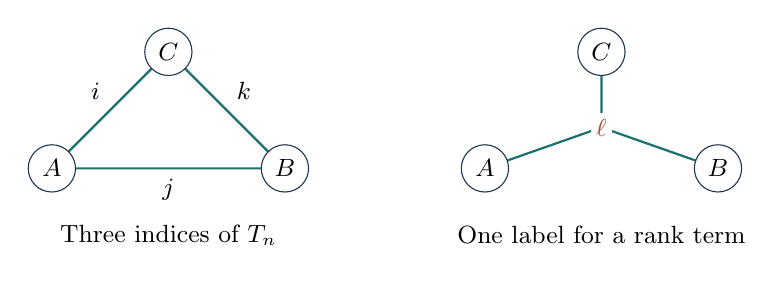
\begin{tikzpicture}[x=1cm,y=1cm,font=\small,
   site/.style={circle,draw=ink,fill=white,minimum size=6mm,inner sep=1.5pt},
   conn/.style={thick,draw=sea}]
  \begin{scope}[xshift=-2.75cm]
   \coordinate (A) at (-1.48,0); \coordinate (B) at (1.48,0);
   \coordinate (C) at (0,1.48);
   \draw[conn] (A)--node[below] {\(j\)} (B)
                --node[above right] {\(k\)} (C)
                --node[above left] {\(i\)} (A);
   \node[site] at (A) {\(A\)}; \node[site] at (B) {\(B\)};
   \node[site] at (C) {\(C\)};
   \node at (0,-.85) {Three indices of \(T_n\)};
  \end{scope}
  \begin{scope}[xshift=2.75cm]
   \coordinate (A) at (-1.48,0); \coordinate (B) at (1.48,0);
   \coordinate (C) at (0,1.48); \coordinate (O) at (0,.52);
   \draw[conn] (O)--(A) (O)--(B) (O)--(C);
   \node[site] at (A) {\(A\)}; \node[site] at (B) {\(B\)};
   \node[site] at (C) {\(C\)};
   \node[fill=white,text=rust,inner sep=2pt] at (O) {\(\ell\)};
   \node at (0,-.85) {One label for a rank term};
  \end{scope}
\end{tikzpicture}
\caption{The three tensor factors correspond to the two inputs and the
output paired against a third matrix. On the left, \(A,B,C\) see
\((i,j),(j,k),(k,i)\). On the right, all three see the same label
\(\ell\in[r]\) and apply their own linear maps.}\label{fig:three-wires}
\end{figure}

The critical ratio occurs at three tips of a tripod with unit arms.
The distances between tips are all two. If the shared-label rate is
\(8/3\), the ratio is \(6/(8/3)=9/4\). Under the strict-saving
hypothesis such a tripod cannot occur. Part~\ref{part:spheres} exploits
this exclusion. If varying the parameters of a tensor were to move
its preferred site in a certain family of prices, the motion would
produce a homogeneous tripod. A rectangular multiplication decoder
first determines the limiting rate when one arm is long. The rigidity
of polynomial multiplication then carries this equality to the tripod
with three equal arms (Proposition~\ref{prop:tripod}). Ruling out that
motion lets us price an entire family of tensors in a single extension
of the sites. This synchronization is the geometric input to compression. Once
the lower bound is proved, we can also identify the three wire lengths
at every price maximizing the value of \(T_n\)
(Corollary~\ref{cor:extremal-price}).

\subsection{From prices to a smaller network}

The family we use consists of sphere tensors. Their entries are
determined by marked points. When these points collide, a tensor
expands into contractions through legs of controlled dimension. Under
the strict-saving hypothesis we can also determine the largest prices
these tensors attain. For prescribed leg widths (logarithms of
dimensions), they attain asymptotically the cost of preparing a
tensor at the cheapest common site and transporting each leg to its
destination (Section~\ref{sec:sphere}). The marked points that specify
the entries and the sites that determine prices play different roles.
Figure~\ref{fig:org} shows how this calculation enters the two parts of
the network construction.

\begin{figure}[!htbp]
\centering
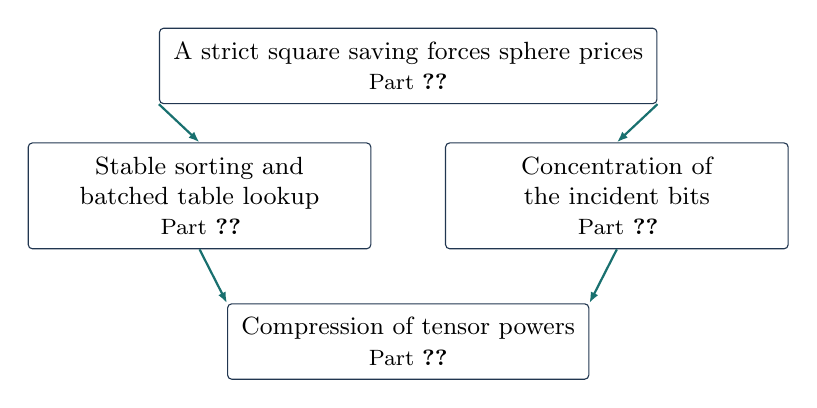
\begin{tikzpicture}[x=1cm,y=1cm,font=\small,
 box/.style={draw=ink,align=center,rounded corners=1.5pt,inner sep=5pt},
 arr/.style={draw=sea,thick,-{Latex[length=4pt]}}]
 \node[box] (price) at (0,0) {A strict square saving forces sphere prices\\
                                  {\footnotesize Part~\ref{part:spheres}}};
 \node[box,text width=4.0cm] (sort) at (-2.65,-1.65)
     {Stable sorting and\\batched table lookup\\{\footnotesize Part~\ref{part:sorting}}};
 \node[box,text width=4.0cm] (conc) at (2.65,-1.65)
     {Concentration of\\the incident bits\\{\footnotesize Part~\ref{part:local}}};
 \node[box] (vol) at (0,-3.5) {Compression of tensor powers\\
                                  {\footnotesize Part~\ref{part:volume}}};
 \draw[arr] (price.south west)--(sort.north);
 \draw[arr] (price.south east)--(conc.north);
 \draw[arr] (sort.south)--(vol.north west);
 \draw[arr] (conc.south)--(vol.north east);
\end{tikzpicture}
\caption{The implication needed for the lower bound. Sorting and
concentration give complementary estimates on the same network.
Repeated compression would violate the independent-list lower bound
of Theorem~\ref{thm:many}.}\label{fig:org}
\end{figure}

The compression must pay for each table of a network and for the
records that say how tables are connected. Direct lookup in a table
of \(u\) incident bits can cost \(2^u\). In a large batch, sorting
queries together with table entries amortizes that cost. Part~\ref{part:sorting}
uses incidence inequalities from sphere tensors to route records.
For \(2^u\) records of width \(O(u)\) the resulting stable sort costs
\(O(u^p)\) per record for some \(p<2\). Wider records admit a separate
estimate that keeps the cost close to linear in their width.

The strict inequality \(p<2\) matters because the quantity controlled
by collisions is proportional to the \emph{square} of a leg width.
Part~\ref{part:local} realizes the wiring with sphere tensors, moves
insertions across their seams and merges them. The use of fermionic contractions to reduce wiring is
related to the crossing construction of~\cite{Khoruzhii,oaG} and to
compression in subexponential satisfiability algorithms~\cite{falseeth,Anthropic}.
Merging concentrates the
incident bits at fewer stations while controlling the sum of squared
widths. Part~\ref{part:volume} applies these identities in rounds.
The expansion has many summands with different wirings. A single
network must describe the possible wirings, route the records, look
up the entries and sum the contributions. Counting all four operations
gives the logarithmic saving in Theorem~\ref{thm:shaving} and completes
the contradiction.

\subsection{Earlier bounds for matrix multiplication}\label{sec:history}

Strassen applied his seven-product identity recursively to blocks, giving
exponent $\log_2 7$~\cite{strassen}. Subsequent algorithms found savings
by working with several matrix products at once. Pan aggregated trilinear
forms~\cite{pan}, Bini showed how interpolation converts approximate
bilinear identities into exact algorithms~\cite{bini}, and Sch\"onhage's
asymptotic sum inequality turned a direct sum of matrix products into an
upper bound on the exponent of a single product~\cite{schoenhage}.
Coppersmith and Winograd studied recursive extraction of disjoint
products~\cite{cw82}. Strassen's laser method extracts them from tensor
powers~\cite{Strassen87}, and Coppersmith and Winograd designed an auxiliary
tensor for which progression-free sets accomplish the extraction~\cite{cw}.

The successive improvements depended on how many products could be kept
independent. Analyses of higher tensor powers~\cite{sto,ds,vw,legall},
refined extraction and asymmetric hashing~\cite{avw,duan,alphaomega,alman},
and numerical optimization~\cite{dupont} sharpened the bounds obtained
from the Coppersmith--Winograd tensor. Staggered extraction gave
$\omega_F<2.371055$ over every field~\cite{stagger}. A separate line of
work embedded matrix products in group algebras~\cite{cohn2003,cohn2005}
and in the algebras of coherent configurations~\cite{CohnUmansSupport}.

The upper bound $9/4$ comes from polynomial multiplication. In Strassen's
asymptotic spectrum~\cite{spectrum}, asymptotic rank is the maximum of
normalized functions that are additive on direct sums, multiplicative on
tensor products and monotone under restriction. Over $\mathbb C$, the
upper-bound proof tracks how these functions value polynomial multiplication
as the two input degrees grow. Degenerations give a lower bound on the
growth of this profile. Interpolation gives an upper bound that depends on
the value at matrix multiplication. Comparing the two bounds yields
$9/4$~\cite[Theorem~1.1]{nine}. The central degeneration separates blocks
that have independent variables on two legs and share the third. Partial
labels and semidirect sums give related formulations of this step
\cite{two258,li}. L\"u proved the separation step in arbitrary
characteristic~\cite{lu}. Amanov, van den Berg and Zuiddam obtained the
bound over every field~\cite[Theorem~1.1]{abvz}. See also the tensor-value
proof~\cite{tensorvalue} and Shpilka's explicit algorithms~\cite{shpilka}.
The rectangular version of the argument~\cite{uznanski,abvz} connects
these estimates to the dual exponent studied in~\cite{coppersmith,alphaomega}.

On the lower-bound side, Bl\"aser proved that the ordinary rank of $T_n$
is at least $\tfrac52 n^2-3n$ over every field~\cite{Blaeser}.
Over $\mathbb C$, Landsberg gave an ordinary-rank bound of
$3n^2-o(n^2)$~\cite{LandsbergRank}, and Landsberg and Micha{\l}ek
gave a border-rank bound of $2n^2-\lceil\log_2 n\rceil-1$
\cite{LandsbergMichalek}. A constant factor above $n^2$ disappears on
taking roots along the sequence $T_n^{\otimes j}\simeq T_{n^j}$.
Barriers for the laser method and bounds from tensor irreversibility
address algorithms that pass through specified intermediate
tensors~\cite{limits,irreversible}. For polynomial multiplication,
Amanov, van den Berg and Zuiddam similarly proved that $9/4$ is optimal
for a specified set of degenerations and combination
rules~\cite[Theorem~5.4]{abvz}. Theorem~\ref{thm:square} gives the
matching lower bound for unrestricted arithmetic circuits. Related
work on the spectrum constructs quantum functionals~\cite{CVZ} and
explicit points over arbitrary fields~\cite{almanlipratt}, and describes
the sublevel sets of asymptotic rank by polynomial
equations~\cite{SpectralSublevels}. Wigderson and Zuiddam survey this
framework~\cite{WZ}.



\clearpage
{\small\tableofcontents}
\clearpage

\section{The obstruction from list distinctness}\label{sec:obstruction}
Fix a finite field \(k\). Consider the test that accepts a list precisely when
its records are pairwise distinct. Sorting gives one way to perform the
test. Our lower bound applies to every tensor network computing it, even
when a single network tests many lists at once. The contradiction will
come from estimating the cost per input bit. A matrix multiplication
exponent below \(9/4\) would drive that cost below the lower bound after
a fixed number of compressions.

\subsection{Two estimates for networks on bits}
A \emph{bit tensor} of arity \(u\) is a function \(\{0,1\}^u\to k\).
In a tensor network each vertex carries such a table. A wire pairs two
argument positions, and each unpaired position is a named exterior bit.
For a fixed setting of the exterior bits, multiply the vertex entries
and sum over all settings of the internal wires. This gives the tensor
represented by the network. A network is \emph{trivalent} if each
vertex has arity at most three. Its \emph{size} counts the vertices and
exterior bits. Its \emph{volume} counts the vertices and all wires,
including the exterior wires. These counts agree up to an absolute
factor by trivalency. For networks of unrestricted arity we count
vertices plus their total arity.

The first estimate starts with an arbitrary trivalent network. Its
conclusion gives a network for a tensor power, with separate exterior
bits for each copy. On these bits it must compute the product of the
original answers.

\begin{theorem}[Compression of tensor powers]\label{thm:shaving}
Suppose \(\omega_k<9/4\). For every \(\eta>0\) there is a \(\gamma>0\)
such that the following holds for all sufficiently large \(n\).
Write \(h=\lceil\log_2 n\rceil\). If a trivalent \(k\)-network of size
\(m\le n^{1.05}\) with \(e\ge n\) exterior bits represents \(V\), then
for some integer \(d\ge1\) its power \(V^{\otimes d}\) has a trivalent
\(k\)-network with \(de\) distinct exterior bits and size at most
\begin{equation}\label{eq:shave}
                   d\big(mh^{-\gamma}+eh^\eta\big).
\end{equation}
Here \(d\le n^{o(1)}\) uniformly in the input network for fixed \(k,\eta\).
\end{theorem}

Section~\ref{sec:shaving} proves Theorem~\ref{thm:shaving}. Per copy,
the first term saves a power of \(h\) on the original size. The second
charges \(h^\eta\) for each exterior bit. The choice of \(\eta\) lets
us compare this charge with the cost of list distinctness.

For \(w\ge1\), let \(D_w\) be the zero-one tensor for a list of \(2^w\)
words of \(2w\) bits each. Its value is one exactly when the words
are pairwise distinct. It has \(n_w=2w\,2^w\) exterior bits. The tensor
\(D_w^{\otimes t}\) tests distinctness separately within each of \(t\)
independently specified lists. The network may connect vertices across
lists. Let \(\operatorname{vol}_k\) denote minimum trivalent volume over \(k\).

\begin{theorem}[Volume of list distinctness]\label{thm:many}
There is a constant \(\sigma>0\), depending only on \(k\), such that for
all sufficiently large \(w\) and every integer \(1\le t\le 2^w\),
\begin{equation}\label{eq:many}
                  \operatorname{vol}_k(D_w^{\otimes t})
                          >t n_w w^\sigma .
\end{equation}
\end{theorem}

Section~\ref{sec:list} proves Theorem~\ref{thm:many}. Its uniformity
in \(t\) is essential because the replication factor in
Theorem~\ref{thm:shaving} is chosen by the compression.

\subsection{Comparison at a fixed input length}
\begin{proposition}\label{prop:finitefield}
Over every finite field \(k\), \(\omega_k\ge 9/4\).
\end{proposition}
\begin{proof}
A sorting network on \(2^w\) records uses \(O(2^w w^2)\) comparisons
\citep{batcher}. Comparing and conditionally exchanging two \(2w\)-bit
words takes \(O(w)\) Boolean gates. After sorting, the conjunction of
the inequalities between adjacent words computes \(D_w\). To realize
this circuit as a tensor network, use the zero-one table of each gate,
copy bits at fan-outs with equality tables, and pin the output to one.
For each accepted input there is exactly one consistent assignment of
the internal wires. This gives a trivalent network over \(k\) of size
\(m_0=O(n_w w^2)\).

Suppose \(\omega_k<9/4\). Choose \(0<\eta<\sigma\), take \(\gamma\)
from Theorem~\ref{thm:shaving}, and fix an integer \(J>2/\gamma\).
Set \(n=n_w\) and \(h=\lceil\log_2 n\rceil=w+O(\log w)\). These
parameters stay fixed through all \(J\) applications of the theorem.
At step \(j\) write \(t_j\) for the number of lists, \(m_j\) for the
network size and \(x_j=m_j/(t_jn)\) for the size per exterior bit.
Initially \(t_0=1\) and \(x_0=O(w^2)\). With replication factor \(d_j\),
\eqref{eq:shave} gives
\[
         t_{j+1}=d_jt_j,\qquad
         x_{j+1}\le h^{-\gamma}x_j+h^\eta .
\]
Inductively, at each of the first \(J\) steps the network has at least
\(n\) exterior bits and \(t_j=n^{o(1)}\), since the bound on \(d_j\)
is uniform and \(J\) is fixed. The recurrence gives
\(x_j=O(w^2+h^\eta)\), so \(m_j=t_j n x_j\le n^{1.05}\) for large \(w\).
This verifies the size hypothesis at each step. Summing the recurrence gives
\[
       x_J \le h^{-J\gamma}x_0+
                     h^\eta\sum_{r=0}^{J-1}h^{-r\gamma}
               = O(w^\eta).
\]
Since \(\log_2 t_J=o(w)\), Theorem~\ref{thm:many} applies to these
\(t_J\) lists. Their network has volume \(O(t_J n w^\eta)\) by
trivalency, which violates \eqref{eq:many} for sufficiently large \(w\).
\end{proof}

\subsection{Passing from finite fields to arbitrary fields}
The step that permits specialization is to extract a single bilinear
identity with a strict rank saving. Its coefficients generate a
finitely generated ring, and its equations survive reduction to a finite field.

\begin{lemma}[Bilinearization of a formal circuit]\label{lem:bilinearize}
If a formal circuit for multiplying two \(s\)-by-\(s\) matrices over
\(F\) uses \(q\) nonscalar multiplication or division gates, then
\begin{equation}\label{eq:gate-rank}
                     \operatorname{rank}_{\overline F}(T_s)\le 2q .
\end{equation}
Here \(q\) counts a multiplication when both inputs are nonconstant and
a division when its divisor is nonconstant.
\end{lemma}
\begin{proof}
Over the infinite field \(\overline F\), choose matrices \(A,B\) at
which all intermediate rational functions are regular and every divisor
is nonzero. Evaluate the circuit on \(A+uX,B+vY\) with \(u^2=v^2=0\).
Each gate has a unique expansion
\[
       f=f_{00}+u f_{10}+v f_{01}+uv f_{11}.
\]
Here \(f_{00}\) is a scalar, \(f_{10}\) is linear in \(X\), and
\(f_{01}\) is linear in \(Y\). At a product gate \(f=ab\), the mixed
coefficient satisfies
\[
        f_{11}=a_{00}b_{11}+a_{11}b_{00}
                         +a_{10}b_{01}+a_{01}b_{10}.
\]
Only the last two terms require new products of linear forms.
At a quotient gate \(f=a/b\), use \(bf=a\) and \(b_{00}\ne0\) to obtain
\[
        b_{00} f_{11}=a_{11}-b_{11}f_{00}-b_{10}f_{01}-b_{01}f_{10}.
\]
This again requires at most two new products. Linear operations,
including multiplication or division by a field scalar, contribute none.
The mixed coefficients of the outputs are the entries of \(XY\).
They all belong to the span of at most \(2q\) products of an
\(X\)-linear form and a \(Y\)-linear form, giving \eqref{eq:gate-rank}.
\end{proof}

\begin{lemma}[Finite specialization]\label{lem:specialize}
If \(\omega_F<9/4\) over a field \(F\), then \(\omega_k<9/4\)
over some finite field \(k\).
\end{lemma}
\begin{proof}
The circuit bound has the form \(O(s^{9/4-\epsilon})\) for some fixed
\(\epsilon>0\). By Lemma~\ref{lem:bilinearize}, at a sufficiently large
side \(s\ge2\) we have a rank decomposition of \(T_s\) over \(\overline F\)
with \(r<s^{9/4}\) terms. Let
\(R\subseteq\overline F\) be the unital ring generated over \(\mathbb Z\)
by all of its coefficients. The decomposition identities are polynomial
equations over \(R\) with target coefficients zero and one.

Choose a maximal ideal of \(R\). Its residue field \(k\) is finitely
generated as a \(\mathbb Z\)-algebra. In positive characteristic Zariski's
lemma makes \(k\) a finite extension of its prime field. In characteristic
zero the same lemma over \(\mathbb Q\) would make \(k\) a number field.
Multiplying its algebra generators by a common positive integer \(M\)
would then make them algebraic integers. Consequently the generated
ring would lie in the ring of integers of \(k\) with \(M\) inverted.
This ring omits \(1/\ell\) for every prime \(\ell\nmid M\), whereas
the field \(k\) contains all of \(\mathbb Q\). Thus \(k\) is finite.
Reducing the identities gives \(\operatorname{rank}_k(T_s)\le r\).

Finally, take the \(j\)-th power of this fixed bilinear algorithm.
Each of the three linear maps can be applied one tensor coordinate at
a time. Since \(s^2\le r\) by flattening rank, every intermediate
array has at most \(r^j\) entries. The linear work and the \(r^j\)
scalar products together cost \(O_{r,s}(j r^j)\) operations at side
\(s^j\). Padding to the next power of \(s\) gives
\(\omega_k\le\log_s r<9/4\).
\end{proof}

\begin{proof}[Proof of Theorem~\ref{thm:square}]
Proposition~\ref{prop:finitefield} and Lemma~\ref{lem:specialize} give
the lower bound over every field. The upper bound over every field is
due to Amanov, van den Berg and Zuiddam \citep{abvz}.
\end{proof}

\subsection{Rank bounds from the exponent}\label{sec:finite-ranks}
We use the passage from an algorithm at one fixed size to an algorithm
on tensor powers, together with the closure argument for border rank
\cite{bini,bcs,spectrum}.

\begin{proof}[Proof of Corollary~\ref{cor:tight}]
Fix \(n\ge2\). A rank-\(r\) decomposition of \(T_{n^j}\) over any field
\(K\) gives \(\omega_K\le\log_{n^j} r\) by the recursion and padding in
Lemma~\ref{lem:specialize}. Theorem~\ref{thm:square} therefore gives
\(\operatorname{rank}_K(T_{n^j})\ge n^{9j/4}\) at each \(j\). Taking
roots gives the asymptotic-rank lower bound. At \(K=\overline F\) and
\(j=1\), Lemma~\ref{lem:bilinearize} now gives the claimed lower bound
of \(\lceil n^{9/4}/2\rceil\) on the number of nonlinear gates.

For the geometric border bound, work in the fixed tensor space \(V\)
over \(\overline F\) containing \(T_n\). Suppose \(T_n\) is in the
Zariski closure of the rank-at-most-\(r\) tensors. For each \(j\),
their \(j\)-th powers span a space containing \(T_n^{\otimes j}\),
since membership of a tensor power in this span is a closed condition.
The number of coefficients of a homogeneous polynomial of degree \(j\)
in \(\dim V\) variables bounds the dimension of the span. We can thus
express \(T_n^{\otimes j}\) using \(O_n(j^{\dim V-1})\) such powers,
each of rank at most \(r^j\). Comparison with the lower bound at
\(n^j\) and passage to \(j\)-th roots give \(r\ge n^{9/4}\).

For the asymptotic-rank upper bound fix \(\varepsilon>0\). At side \(n^j\)
the known circuit upper bound and Lemma~\ref{lem:bilinearize} give a
decomposition of rank \(r_j=O_{F,\varepsilon}(n^{j(9/4+\varepsilon)})\)
over \(\overline F\). Its coefficients belong to a finite extension
\(E_j/F\), of degree \(d_j\). For each \(t\), power this decomposition
\(t\) times. Expand each of the three vectors in each simple tensor
in an \(F\)-basis of \(E_j\) containing \(1\), then project the
products of basis coefficients onto the coordinate of \(1\).
The tensor being represented is defined over \(F\), so this gives
\[
        \operatorname{rank}_F(T_n^{\otimes jt})\le d_j^3 r_j^t .
\]
The limit defining asymptotic rank exists by submultiplicativity.
First take \(jt\)-th roots and let \(t\to\infty\) with \(j\) fixed.
Then let \(j\to\infty\) and \(\varepsilon\downarrow0\). The resulting
upper bound is \(n^{9/4}\) over the original field.
\end{proof}

At finite sizes, Corollary~\ref{cor:tight} also conflicts with the dyadic
border-rank estimate proposed in the first version of Sun's
preprint~\cite{Sun}. At $n=2^8$ the proposed upper bound is $2^{17}$
and our lower bound is $2^{18}$.

The square tensor also decides a prediction about tight three-tensors.
A support is tight when each local basis admits distinct integer
weights whose sum is zero on every support triple. In \(T_n\), take
\(B>n\) and assign weights \(i-Bj\), \(Bj-B^2k\) and \(B^2k-i\)
to \(e_{ij},e_{jk},e_{ki}\), respectively. Each assignment is
injective on its factor and the three weights sum to zero. Each
one-factor flattening has rank \(n^2\). Strassen's conjecture for
tight tensors predicts asymptotic rank \(n^2\) in this case
\cite[Conjecture~5.3]{Strassen1994}. Corollary~\ref{cor:tight}
gives \(n^{9/4}\).

\begin{proof}[Proof of Corollary~\ref{cor:rectangular}]
The three one-factor flattenings have ranks \(ab,bc,ca\).
These are lower bounds for geometric border rank by the closedness
of matrix-rank conditions, and for asymptotic rank by multiplicativity
of flattening ranks. Grouping corresponding factors in
\[
            T_{a,b,c}\otimes T_{b,c,a}\otimes T_{c,a,b}
                                \simeq T_{abc}
\]
turns each of the three indices into a tuple with \(abc\) possibilities.
Both ranks are invariant under cyclic relabeling of the factors and
submultiplicative under tensor product. Hence each of their values
on \(T_{a,b,c}\), cubed, is at least \((abc)^{9/4}\) by
Corollary~\ref{cor:tight}. The case \(abc=1\) is immediate.

For \(a=c=n\) and \(b=\lfloor n^\beta\rfloor\), the geometric border
bound is \(\Omega(n^{3(2+\beta)/4})\). The bilinearization in
Lemma~\ref{lem:bilinearize} applies entrywise to rectangular products
as well. A quadratic exponent therefore requires \(3(2+\beta)/4\le2\).
This gives \(\alpha_F\le2/3\), and the upper bound for multiplication
at \(\beta=1/2\) gives \(\alpha_F\ge1/2\)~\cite{abvz}.
\end{proof}

\section{Tensor prices and wire distances}\label{sec:prices-background}
A bilinear algorithm of rank \(r\) constructs its tensor from \(r\)
independent scalar products by local linear maps. A \emph{spectral
point} assigns a value to tensors that can only decrease under such
maps. Tensoring multiplies the values, so their logarithms add. We call
these logarithms \emph{prices}. Applied to a wire, the price measures
the cost of sharing an index between its two sites. This is how a
spectral point gives a geometry on the sites of a tensor network.

\subsection{From tensors to distances}
Fix a field and a finite set \(S\) of at least two sites. Each tensor
has one finite-dimensional vector space at each site. A tensor \(T\)
is a \emph{restriction} of \(U\) if one linear map at each site takes
\(U\) to \(T\). For a tensor product, group the factors at each site.
For a direct sum, take the direct sum of the spaces at every site, so
the two tensors occupy separate blocks. The unit \(\mathbf 1\) is the
tensor \(1\) in one-dimensional spaces.

A spectral point \(\varphi\) is a restriction-monotone map to
\(\mathbb R_{\ge0}\) that preserves zero and the unit and satisfies
\[
     \varphi(T\oplus U)=\varphi(T)+\varphi(U),\qquad
     \varphi(T\otimes U)=\varphi(T)\varphi(U).
\]
Every nonzero tensor restricts to \(\mathbf 1\), so its value is at least
one. The price at scale \(D>0\) is \(H(T)=D\log\varphi(T)\), with
\(H(0)=-\infty\). In this section and Part~I logarithms are natural.
Thus the prices of~\cite{oaG} are multiplied by \(\log 2\) at the same scale.

For a nonempty \(A\subseteq S\), the tensor
\[
         \Delta_A(q)=\sum_{j=1}^q\bigotimes_{i\in A} e_j
\]
shares a \(q\)-valued index among the sites of \(A\). Its other legs are
one-dimensional. Tensoring diagonals multiplies their dimensions, and a
local projection can discard any set of labels. Comparing powers of
dimensions \(q\) and \(2\) therefore gives
\[
            H(\Delta_A(q))=\delta(A)\log q,\qquad q\ge2.
\]
We call \(\delta(A)\) the common-label rate on \(A\). In particular
\(\Delta_S(q)\) is a direct sum of \(q\) units, so \(\delta(S)=D\).
For \(a\ne b\), \(\Delta_{\{a,b\}}(q)\) is a wire of dimension \(q\).
Write \(d(a,b)=\delta(\{a,b\})\) and set \(d(a,a)=0\).
For example, matrix rank across a fixed cut of \(S\) is a spectral
point. At scale one its wire distance is one for sites on opposite
sides of the cut and zero for sites on the same side.

Joining two wires by contracting their common endpoint gives a wire
between their other endpoints. Monotonicity and additivity of price
give the triangle inequality for \(d\). A \(q_i\)-dimensional wire
can also move a leg of dimension \(q_i\) from \(x_i\) to \(y_i\).
Moving each leg of a nonzero tensor \(T\), then applying the same
argument in reverse, gives the transport bound
\begin{equation}\label{eq:prices-transport}
       |H(T;x)-H(T;y)|\le\sum_i d(x_i,y_i)\log q_i .
\end{equation}
Here \(x=(x_i)\) and \(y=(y_i)\) are the placements of the legs. Group
the legs assigned to one site. When all legs are at a single site, any
nonzero tensor there is equivalent to the unit and has price zero.

\subsection{Geometric extension and spectral comparison}
A \emph{spectral space} is a metric space with compatible prices for
all finite placements, whose wire rates are the given distances.
Compatibility allows trivial legs to be added and legs at coincident
sites to be grouped. On a finite set of positive diameter the scale is
its common-label rate, which may vary with the set. At a single point the
scale is zero. Identifying sites at zero wire distance turns a spectral
price on finitely many sites into a spectral space.

Every spectral space embeds, with all its prices, in a complete
\(\operatorname{CAT}(0)\) spectral space. In the extension every pair
\(a,b\) has a unique midpoint \(m\), and every point \(o\) satisfies
\[
      d(o,m)^2\le \tfrac12 d(o,a)^2+\tfrac12 d(o,b)^2
                                      -\tfrac14 d(a,b)^2 .
\]
Prices are jointly convex as their legs move along geodesics. Distances
and prices may be rescaled together. In a pointed metric ultralimit
of these spaces, the price of a fixed tensor on a bounded sequence of
placements is the ultralimit of its prices
\citep[Sections~\ext{G}{sec:spectra} and~\ext{G}{sec:limits},
Theorem~\ext{G}{thm:geometry} and Proposition~\ext{G}{prop:joint-convexity}]{oaG}.
We also use convexity of distance and nonexpansiveness of nearest-point
projection onto a nonempty closed convex set. A finitely supported
probability measure has a unique barycenter \(b\) minimizing its mean
squared distance. Evaluating the same mean at \(z\) increases it by at
least \(d(z,b)^2\) \citep{BridsonHaefliger,oaG}.

Over an algebraically closed field, price sublevel sets in a fixed tensor
format are Zariski closed. Under a field extension, the possible joint
values of spectral points on tensors defined over the original field
are preserved \citep[Section~\ext{G}{sec:spectra}]{oaG}.
Finally, if two nonzero tensors on the same sites satisfy
\(\varphi(T)<\varphi(U)\) for every spectral point, there is a fixed
integer \(C\) such that, for every \(j\ge1\), \(T^{\otimes j}\)
is a restriction of the direct sum of \(C\) copies of \(U^{\otimes j}\).
We use this strict form of spectral comparison to turn price inequalities
into exact tensor restrictions \citep[Lemma~\ext{G}{lem:spectral-comparison}]{oaG}.

\section{The cost of testing many lists}\label{sec:list}

Two distinctness tests suffice to check that records have reached their
specified destinations. This gives a common starting point for the two
cases of Theorem~\ref{thm:many}. In a field without ports, the possible
destinations force many wires to have large total length in a suitable
spectral space. In a finite field with ports, cheap distinctness tests
would make it possible to compress a family of tensors with a known
lower bound.

\subsection{Checking a tagged permutation}

Write \(h=w-1\), \(N=2^h\), and index records by the \(h\)-bit words.
The tagged-permutation tensor \(\operatorname{Tag}(h,h)\) of
\cite[Definition~\ext{G}{def:tag}]{oaG} takes
\(N\) records \((j_i,x_i)\) and an ordered list of \(N\) payloads
\(y_j\), with \(h\) bits per tag or payload. Its value is one when
\(i\mapsto j_i\) is a permutation and \(x_i=y_{j_i}\) for every \(i\).
Its other entries are zero.

The first \(D_w\) test checks the tags. Encode each \(j_i\) as
\((0,j_i,0^{h+1})\) and fill the remaining \(N\) positions with the
distinct words \((1,j,0^{h+1})\). All \(2N\) words have length \(2w\),
and the test passes precisely when the tags form a permutation \(\pi\).

The second \(D_w\) test checks the payloads. Its first \(N\) words are
\((j_i,0,x_i,0)\). At the position for \(j\) in the second half, sum
over two choices, the reserve word \((j,1,0^h,0)\) with weight \(1\)
and the comparison word \((j,0,y_j,0)\) with weight \(-1\).
For tags forming \(\pi\), the only possible collision at address \(j\)
is between the comparison word and the word from \(i=\pi^{-1}(j)\).
Thus the signed sum factors as
\[
     \prod_j \bigl(1-\mathbf 1_{\{x_{\pi^{-1}(j)}\ne y_j\}}\bigr)
       =\prod_j\mathbf 1_{\{x_{\pi^{-1}(j)}=y_j\}} .
\]
This identity holds in every characteristic. A summed selector bit for
each address controls its word and its weight. Copying the tags,
selecting the words, and pinning the constants cost \(O(Nh)\) trivalent
volume. Consequently, if \(D_w^{\otimes t}\) has a realization of
volume \(V\), two uses of that realization give a network for
\(\operatorname{Tag}(h,h)^{\otimes t}\) of volume at most
\(2V+O(tNh)\), including when the realization shares work among lists.

\subsection{Fields without ports}

A class of Hadamard spaces has \emph{ports} if it admits regular
graphs of unbounded order and common bounded degree with the following
property. For every placement of their vertices into any space of the
class, the mean squared distance of two independent uniform vertices
is at most a fixed constant times the mean squared edge length.
A field has ports when its Hadamard spectral spaces have this property
\cite[Definition~\ext{G}{def:ports}]{oaG}.

\begin{lemma}[Uniform destinations]\label{lem:uniform-demand}
Let the field have no ports. Consider a fixed trivalent topology with
\(r\) input bits and \(r\) output bits. Suppose that for every permutation
in the support of a distribution, some choice of vertex tables realizes
the \(r\) independent wires joining each input to its assigned output.
If each input has a uniform destination on a set of \(q\ge2\) outputs,
the topology has size \(\Omega(r\sqrt{\log q})\). The destination sets
may depend on the input.
\end{lemma}

\begin{proof}
Give each exterior bit its own equality leaf. Connect the resulting
components in a path by adding edges to the graph used to measure
distances. This increases the maximum degree by at most two and gives
\(m\) edges, with \(m\) at most a constant times the network size.
Let \(\alpha\) be the law of a uniform oriented edge, and let \(\mu\)
be the joint law of a uniform input and its random destination.
For any placement in a spectral space with distance \(d\),
\[
                    r\,\mathbb E_\mu d\ \le\ m\,\mathbb E_\alpha d .
\]
Indeed, for each permutation the network tensors locally contract
the product of its internal bit wires to the prescribed exterior
wires. Monotonicity and additivity of prices bound the sum of the
destination distances by the sum of the internal edge lengths.
Average over the permutations and include the extra edges on the right.

We need a placement where many destinations are far away at once.
The class of Hadamard spectral spaces is closed under isometry,
rescaling, closed convex subspaces, and pointed ultralimits
(Section~\ref{sec:prices-background}). The product theorem
\cite[Theorem~\ext{P}{prod:main}]{oaP} gives a subclass with the same
properties and no ports, closed also under finite \(\ell_2\) products.
Let \(\mathcal K\) be the squared distance tables \(D=d^2\) realized
in this subclass with \(\mathbb E_\alpha D\le1\). Products of rescaled
placements give convex combinations of tables. Connectivity bounds
every entry, and pointed ultralimits realize coordinatewise limits.
Hence \(\mathcal K\) is convex and compact.

For a probability law \(\nu\le 2\mu\) on ordered pairs, let
\(\beta_\nu=\max_{D\in\mathcal K}\mathbb E_\nu D\). By rescaling,
\(\mathbb E_\nu d^2\le\beta_\nu\mathbb E_\alpha d^2\) for every
placement in the subclass. Write \(X,Y\) for the endpoints under
\(\nu\). The graph entropy bound \cite[Corollary~\ext{P}{cor:graph-entropy}]{oaP}
and the bounded degree of our graph give
\(H_\nu(Y\mid X)\le C(1+\beta_\nu)\), with entropy in bits.
Every pair has \(\nu\)-mass at most \(2/(rq)\), so
\[
    H_\nu(Y\mid X)=H_\nu(X,Y)-H_\nu(X)
               \ge \log_2(rq/2)-\log_2 r=\log_2(q/2).
\]
It follows that \(\beta_\nu\ge c\log q\) for all sufficiently large
\(q\), uniformly in \(\nu\).

Bilinear minimax on \(\mathcal K\) and the compact convex set of
laws \(\nu\le2\mu\) gives a single \(D=d^2\in\mathcal K\) for which
\(\mathbb E_\nu D\ge c\log q\) for every such law. If the pairs with
\(D<c\log q\) had \(\mu\)-mass at least \(1/2\), conditioning \(\mu\)
on those pairs would violate this bound. Hence
\(\mathbb E_\mu d\ge \tfrac12\sqrt{c\log q}\), while
\(\mathbb E_\alpha d\le1\) by Cauchy--Schwarz. The price inequality
gives the result. For bounded \(q\), counting exterior bits suffices.
\end{proof}

In a network for \(\operatorname{Tag}(h,h)^{\otimes t}\), pin each
list's tags to a uniform permutation. The topology realizes a permutation
of \(r=tNh\) payload bits. Each input bit has \(q=N\) possible
destinations, at its own bit position in its own list, all equally
likely. By Lemma~\ref{lem:uniform-demand},
\(2V+O(tNh)\ge c\,tNh\sqrt h\). Since \(n_w=4N(h+1)\), this proves
\eqref{eq:many} for any fixed \(0<\sigma<1/2\) and all sufficiently
large \(w\), uniformly in \(t\).

\subsection{Finite fields with ports}

Fix a finite field with ports. We use the signed counting tensor
\(U_\ell^*\) on \(\ell\) exterior bits from the circuit lower-bound
paper. Its entries count the signed computation paths of a polynomially
clocked universal machine, reduced in the field. The polynomial-size
verifier gives an exact trivalent network of size \(\ell^{O(1)}\) for
one copy. Sum over its guess strings, requiring the unused bits on
each computation path to be zero, and weight the outcome by its sign. The exact batch lower bound
\cite[Theorem~\ext{P}{thm:batches}]{oaP} gives \(\delta,\xi>0\)
such that, for all sufficiently large \(\ell\),
\[
       \operatorname{vol}_k\bigl((U_\ell^*)^{\otimes j}\bigr)
              >j\ell^{1+\delta}
       \qquad (1\le j\le 2^{\ell^\xi}).
\]

The descent with tagged permutations
\cite[Proposition~\ext{G}{prop:oracle-descent}]{oaG} supplies a
constant \(a>0\). For all sufficiently large \(h\), given a trivalent
network of size \(s\) in the range \(N\le s\le N^4\), with \(e\)
exterior bits, it constructs a network for \(d\) copies of its tensor
using trivalent gates and \(\operatorname{Tag}(h,h)\) tests. Its size
\(S\), charging every incident bit including those at tests, satisfies
\[
            S\le C d\bigl(sh^{-a}+e(\log h)^C\bigr),
           \qquad \log_2 d=O\bigl((\log h)^2\bigr).
\]
These bounds are uniform in the network. The normalization required
for descent attaches equality leaves and subdivides self-loops. It
costs only a constant factor, and the cited bound holds on every fixed
polynomial size range.

Choose \(b>\max\{2,2/\xi\}\) and
\(0<\sigma<\min\{a/4,b\delta/4,1/4\}\). Suppose there are arbitrarily
large \(w=h+1\) for which some \(1\le t\le 2N\) admits a realization
of \(D_w^{\otimes t}\) of volume at most \(tn_w w^\sigma\).
The two-list construction gives a network for \(t\) tagged-permutation
tests of size \(O(tNh^{1+\sigma})\).

Group the tests in a descent network into batches of \(t\) and
substitute this realization for each batch. In the last batch pin
unused tests to the identity permutation with zero payloads, where
each has value one. Since the substituted network realizes the full
product tensor, the replacement stays exact under every contraction
of the surrounding wires, including wires joining tests in one batch.
Each full batch contributes \(3tNh\) incident bits to \(S\).
Paying separately for the last batch therefore gives trivalent size
\[
                     O\bigl(h^\sigma S+tNh^{1+\sigma}\bigr).
\]

Set \(\ell=\lceil h^b\rceil\) and begin with \(j=N^2\) copies of
the polynomial-size network for \(U_\ell^*\). At each descent let
\(x=s/(j\ell)\) be the size per exterior bit. The new batch has \(dj\)
copies. Its size per bit, for all sufficiently large \(h\), satisfies
\[
 \begin{split}
 x'&\le C'\left(h^{-a+\sigma}x+
        h^\sigma(\log h)^C+\frac{tNh^{1+\sigma}}{dj\ell}\right)\\
   &\le h^{-a/2}x+h^{2\sigma}.
 \end{split}
\]
Here \(j\ge N^2\), \(d\ge1\), and \(t\le 2N\), so the fraction is
\(O(h^{1+\sigma-b})\). This is the reason for starting with \(N^2\)
copies.

Initially \(x\le h^A\) for some fixed \(A\). Choose a fixed integer
\(L>2A/a\). At every one of these \(L\) steps, the product of the
replication factors is \(N^{o(1)}\). Inductively, \(j=N^{2+o(1)}\)
and \(x\) stays polynomial in \(h\), so the current network and its
normalization have size in the descent range. Iterating the last
inequality gives \(x=O(h^{2\sigma})\). Now \(j\le 2^{\ell^\xi}\)
because \(\log_2 j=(2+o(1))h\), while
\(h^{2\sigma}=o(\ell^\delta)\) by the choice of \(\sigma\).
The final trivalent volume is therefore \(o(j\ell^{1+\delta})\),
contradicting the exact batch lower bound. This proves
Theorem~\ref{thm:many} in the remaining case.


\par\needspace{13\baselineskip}
\part{Sphere tensors and their prices}\label{part:spheres}
\section{Price extensions and simultaneous minimization}\label{sec:prices}

The compression argument introduces new sites at which to place tensor
legs. A price on the old sites already puts a lower bound on the price
of any proposed placement. Contract the legs at the new sites and
evaluate the tensor that remains. One can do this on any tensor power,
with each new site contracting all its copies at once.
Theorem~\ref{thm:extension} shows that these lower bounds are sharp and
gives a criterion for satisfying several price bounds at the same
placement. In Section~\ref{sec:sync} the tensors to be placed will
depend on a parameter. To control specialization of that parameter,
we prove the criterion over valued fields. For a product of ordinary
wires incident to one new site, the minimum is computed in
\cite[Theorem~\ext{G}{thm:extension}]{oaG}.

\subsection{Integral restrictions}
Let \(K\) be a field with a real additive nonarchimedean valuation
\(\nu\), normalized by \(\nu(0)=+\infty\). Its valuation ring is
\(\mathcal O=\{c\in K:\nu(c)\ge0\}\). We use the given coordinate bases
at all sites. A restriction is \emph{integral} if each local matrix has
entries in \(\mathcal O\). A \emph{valued price} \(p\) of scale \(D>0\) on \(S\)
(here $|S|\ge2$, as before) is real on nonzero tensors, has \(p(0)=-\infty,\ p(\mathbf1)=0\), and
is nonincreasing under integral restriction. Its scalar, product, and
direct-sum rules are
\begin{equation}\label{eq:prices-axioms}
 \begin{gathered}
 p(cT)=p(T)-\nu(c) \quad(c\ne0), \qquad
 p(T\otimes U)=p(T)+p(U),\\
 p\Bigl(\bigoplus_j T_j\Bigr)=D\log\sum_j e^{p(T_j)/D}.
 \end{gathered}
\end{equation}
Here \(\log\) is the natural logarithm. Thus multiplying by a scalar of
positive valuation lowers the price. The trivial valuation recovers
ordinary prices.

We shall construct prices using a convenient equivalent form of the
direct-sum rule. For tensors in common spaces, the right side of
\eqref{eq:prices-axioms} bounds \(p(\sum_j T_j)\) by local addition
of blocks. Conversely, suppose this ordinary sum bound holds and
\(p(\Delta_S(q))=D\log q\) for every \(q\). The block inclusions
express \(\bigoplus_j T_j\) as an ordinary sum and give the desired
upper bound. For the lower bound, take the \(m\)-th power of the direct
sum and project at every site onto the words in which the \(j\)-th
summand occurs \(m r_j\) times. Local permutations identify the
result with \(\bigotimes_jT_j^{\otimes m r_j}\) times a diagonal of
size \(m!/\prod_j(mr_j)!\).
For rational probability vectors \(r\) on the nonzero summands,
take \(m\) through multiples of a common denominator. The price per copy
is at least \(\sum_jr_jp(T_j)-D\sum_j r_j\log r_j\).
Maximization gives the asserted identity.

Write \(q_i\) for the local dimensions of \(T\) and \(\nu_{\min}(T)\)
for the minimum valuation of an entry. For \(T\ne0\),
\begin{equation}\label{eq:prices-range}
 -\nu_{\min}(T)\le p(T)\le -\nu_{\min}(T)+D\sum_i\log q_i.
\end{equation}
For the lower bound project to an entry of minimum valuation. For the
upper bound expand \(T\) in at most \(\prod_iq_i\) coordinate tensors
and use the ordinary sum inequality. Thus prices of fixed
scale form a compact space in the topology of pointwise convergence,
since their axioms are closed in the product of the intervals
\eqref{eq:prices-range}. The wire and transport rules above require only
integral operations and hold also for \(p\). At one site the price of a
nonzero vector is \(-\nu_{\min}\), since after division by a minimum-valuation
entry it is integrally equivalent to the unit. When \(K\) contains a
trivially valued field \(F\), restriction to tensors
over \(F\) gives the ordinary spectral geometry of the wire distances.

\subsection{A test for extending a price}
Fix \(p\) on \(S\), and adjoin a finite set \(L\) of sites. Denote by
\(\widehat p\) an extension to \(S\sqcup L\) of the same scale which
retains \(p\) on tensors with trivial legs at \(L\). Such extensions
exist by placing the added sites at old ones. Restriction to any intermediate
list of sites containing \(S\) gives a valued price of scale \(D\).
Indeed the diagonal on that list restricts to the base diagonal and is a
restriction of the full diagonal, so the diagonal test applies. 

A \emph{closure} applies one integral linear functional at each site of
\(L\) and leaves all base legs free. The \emph{assisted cost} of \(T\) is
\begin{equation}\label{eq:prices-beta}
 \beta_p(T)=\sup_{m\ge1}\frac1m
       \sup_{\ell}p\bigl(\ell(T^{\otimes m})\bigr).
\end{equation}
At a site of dimension \(q\) the functional in this formula acts on
\(K^{q^m}\), so it may couple the \(m\) copies arbitrarily. Every
extension satisfies \(\widehat p(T)\ge\beta_p(T)\) by monotonicity
under closure and additivity on powers.

For example, in the ordinary case take the product of two size-\(q\) wires
from \(a\) to \(y\) and from \(y\) to \(b\), where \(a,b\) are old sites
and \(y\) is new. Already on one copy, closing the two legs at \(y\) by
the pairing \(e_i\otimes e_j\mapsto\delta_{ij}\) recovers the wire from \(a\)
to \(b\). This gives the lower bound \(d(a,b)\log q\) for the product. Placing
\(y\) at \(a\) attains it. More generally, placing \(y\) anywhere on
the geodesic from \(a\) to \(b\) attains the bound by additivity of
distance along that segment.

\begin{theorem}[Price extension]\label{thm:extension}
For every tensor \(T\) on \(S\sqcup L\),
\(\beta_p(T)=\min_{\widehat p}\widehat p(T)\).
For an arbitrary family of nonzero tensors \(T_i\) and real numbers
\(h_i\), a single extension satisfies \(\widehat p(T_i)\le h_i\)
for all \(i\) if and only if
\begin{equation}\label{eq:prices-product-test}
 \beta_p(T_{i_1}\otimes\cdots\otimes T_{i_j})
 \le h_{i_1}+\cdots+h_{i_j}
\end{equation}
for every finite list of indices, with repetitions allowed.
\end{theorem}

\begin{proof}
\emph{Minimizing one tensor.}
The zero tensor is immediate. For a prescribed nonzero \(T\) we first
assign prices to a finite list of distinct nonzero tensors \(A_1,\ldots,A_s\)
containing \(T\). The exponents of their mixed products will serve as
variables. For \(x\in\mathbb Q_{\ge0}^s\) set
\[
 b(x)=\frac1n\beta_p\Bigl(\bigotimes_i A_i^{\otimes nx_i}\Bigr),
 \qquad nx\in\mathbb Z^s.
\]
In \eqref{eq:prices-beta} the supremum can be restricted to multiples
of any given integer by repeating each closure independently. Thus assisted
cost is homogeneous under powers and \(b\) is well defined.
Independent closures, taken at common multiples, make \(b\)
superadditive, hence concave by homogeneity.

The increment per unit of coordinate \(i\) lies in the price interval
\eqref{eq:prices-range} for \(A_i\). For the lower estimate isolate a
minimum-valuation coefficient of every added factor, by coordinate
projections at the base sites as well as the added sites. For the upper
estimate expand each added factor in coordinates. Even for a closure
coupling all copies, fixing the added indices of each term induces an
integral closure on the old factors. The coordinate factors remaining at
base sites have price zero, and the ordinary sum bound pays at most
\(D\sum_j\log q_j\) per added factor of format \((q_j)\).
This proves the increment bounds after taking powers. In particular \(b\)
extends continuously to the real orthant.

At a strictly positive rational \(x\) choose a supporting linear form
\(u\) for this homogeneous concave function, so that
\(b(y)\le u\cdot y\) and \(b(x)=u\cdot x\).
The two-sided increment estimates bound \(u_i\) in the same price
interval. We claim that the numbers \(u_i\) respect the price relations on the
list. For example, if \(A_i=A_j\otimes A_k\), then
\(b(x+t(e_j+e_k-e_i))=b(x)\) for both signs of sufficiently small
rational \(t\). The supporting inequality in these two directions forces
\(u_i=u_j+u_k\). A scalar change shifts \(b\) by minus its valuation
per copy, giving the scalar relation by the same argument. If \(A_i\)
restricts integrally to \(A_j\), replacing copies of \(A_j\) by
copies of \(A_i\) can only increase \(b\). The supporting inequality
in the direction \(e_i-e_j\) therefore gives \(u_i\ge u_j\).
A base tensor increases \(b\) by its exact price per unit,
since its factors pass unchanged through every closure.
For \(\Delta_{S\sqcup L}(q)\), closing its added legs by all-ones
functionals yields \(\Delta_S(q)\), and expanding its \(q\) diagonal
entries gives the reverse bound. Thus its increment is \(D\log q\).

To check the ordinary sum bound, let \(A_i=A_j+A_k\) in the list.
Expand \(n\sigma\) copies of \(A_i\) in a product with multiplicities
\(nx\), for a rational \(0<\sigma\le x_i\). A term choosing \(a\)
copies of \(A_j\) has price after closure at most
\(n u\cdot x-n\sigma u_i+a u_j+(n\sigma-a)u_k\).
The ordinary sum bound on the base and the binomial formula bound
the price after closure of the original tensor by
\[
 n u\cdot x-n\sigma u_i+
 n\sigma D\log\bigl(e^{u_j/D}+e^{u_k/D}\bigr).
\]
Taking the supremum per \(n\) through admissible multiples yields
\(b(x)=u\cdot x\) on the left. This proves the required bound on \(u_i\).
Relations involving zero summands hold automatically.

Let \(x\) tend to the unit vector corresponding to \(T\). The support
vectors have a convergent subsequence and continuity gives
\(u_T=\beta_p(T)\) in the limit. Every finite collection of price
relations and the equality at \(T\) is therefore feasible by applying the
construction to the list of all tensors occurring in those constraints.
Compactness of the product of intervals gives a simultaneous
solution for all such relations. The diagonal test following
\eqref{eq:prices-axioms} makes this solution a valued price. This proves
attainment for one tensor.

\smallskip\noindent
\emph{Satisfying several bounds.}
Any extension obeying the proposed bounds satisfies
\eqref{eq:prices-product-test} by additivity on products. Conversely,
take a finite list of \(k\) bounds. Form \(U\) as a direct sum of
\(N_i\) copies of \(T_i^{\otimes n}\) for each \(i\). In a power of
\(U\) each word of summands is a mixed product. Restricting a closure
to the blocks of that word gives an integral closure, whose price is
bounded by \eqref{eq:prices-product-test}. Sum over the words on the
base and take the supremum per copy to obtain
\[
 \beta_p(U)\le D\log\sum_i N_i e^{nh_i/D}.
\]
Choose \(C>\max_i h_i\) and \(N_i=\lceil e^{n(C-h_i)/D}\rceil\).
These multiplicities bring every \(N_i e^{nh_i/D}\) into the interval
\([e^{nC/D},2e^{nC/D}]\). At an extension minimizing \(U\), the
direct-sum identity then gives
\[
 D\log N_i+n\widehat p(T_i)\le\beta_p(U)\le nC+D\log(2k),
 \qquad
 \widehat p(T_i)\le h_i+\frac{D\log(2k)}{n}.
\]
Let \(n\) tend to infinity and apply compactness, first to the finite
list and then, by the finite intersection property, to the whole family.
\end{proof}

Two consequences will be used below. Given several extensions of \(p\),
there is a single extension whose evaluations are bounded above by any
fixed convex combination of theirs. Indeed, each extension bounds
the assisted cost of every mixed product, so the averaged bounds pass
\eqref{eq:prices-product-test}. We may also enlarge the base before
applying the test. Suppose an enlarged base carries a price agreeing
with \(p\) on the old base. A tensor supported on the old base and the
unknown sites has exactly the same closures, with trivial legs on the
extra base sites. Thus its assisted cost is unchanged. This observation
also applies when the enlarged base has larger scale. Theorem~\ref{thm:extension}
then gives an extension at that larger scale.

\subsection{Geodesic placement}
Assume henceforth in this section that \(K\) contains a trivially valued
subfield \(F\). Given pairs of sites \(a_j,b_j\),
place new sites \(y_j\) first at the \(a_j\) and then at the \(b_j\).
The interpolation consequence of Theorem~\ref{thm:extension} gives an
extension bounding the price of every tensor by the affine interpolation
of these two evaluations, with weights \(1-\theta,\theta\). In particular
\[
 d(a_j,y_j)\le\theta\,d(a_j,b_j),\qquad
 d(y_j,b_j)\le(1-\theta)d(a_j,b_j).
\]
The triangle inequality forces equality in both bounds. Thus \(y_j\)
is the point a fraction \(\theta\) of the way along the geodesic from
\(a_j\) to \(b_j\) in a complete \(\operatorname{CAT}(0)\) spectral
realization over \(F\). The same extension provides the interpolation
bound for all tensors over \(K\).

\begin{lemma}[Geodesic determination and submean inequality]\label{lem:geodesic}
Ordinary price data on any subset of a complete
\(\operatorname{CAT}(0)\) spectral space determine all prices on its
closed geodesic convex hull up to a price-preserving isometry fixing the
given data. Moreover, suppose the prices at a central placement are at
most the weighted average of prices at finitely many end placements, for
every tensor on the original slots. In each placement adjoin points
on corresponding geodesic segments. If the two distances of each new
point to its endpoints at the center are the weighted averages of their
values at the ends, the price inequality holds on the enlarged placements.
\end{lemma}

\begin{proof}
For each new site, prescribe the prices of its size-two wires to its
two endpoints. These prices are the two geodesic distances multiplied
by \(\log 2\). We claim that the price of any \(T\ne0\) on the enlarged
list is the smallest number \(h\) for which the bound \(h\) and all the
wire bounds pass the product test. The actual price passes by closure.
Conversely, enlarge the base to include the actual geodesic points,
and apply Theorem~\ref{thm:extension} to duplicate sites with those
bounds. In a common metric realization, the triangle inequality forces
both endpoint distances of each duplicate to be the prescribed distances.
Uniqueness of geodesics identifies the duplicate with the actual point.
Transport~\eqref{eq:prices-transport}
therefore gives the assertion. For a collapsed base all its prescribed
segments are constant and the assertion follows directly.

Iterating this characterization determines prices, including distances,
on all finite geodesic constructions. Completing their union gives the
closed convex hull by continuity of geodesic interpolation, and
\eqref{eq:prices-transport} extends the price identifications to the
completion. An infinite original subset causes no change since each
finite construction starts from finitely many points.

For the second assertion, a collapsed central placement is immediate.
Otherwise fix a product in the test, a power and a closure on its new
sites. The original submean inequality bounds the central price of the
closed tensor by the average of its closed prices at the ends. At each
end this is at most the price of the unclosed power by restriction,
including a collapsed end, where every nonzero tensor has price zero.
Divide by the power and take the supremum at the center. The averaged
actual upper bounds on the enlarged placements thus pass the product
test at the center, and the averaged wire bounds agree with the
prescribed ones there. Apply the characterization just proved.
\end{proof}

\subsection{Unique evaluations at minimizing sites}
A price minimum can admit several placements, as the two-wire example
shows. To compare minimizers as a parameter varies, we add a strictly
convex penalty at each unknown site. Fix \(o\) on the base. For a new
site \(y\), form the direct sum of \(\mathbf1\) and the size-two wire
from \(o\) to \(y\). Its direct-sum label is visible at every site in
the configuration, so its price is
\[
 f(r)=D\log\bigl(1+\exp(r\log(2)/D)\bigr),\qquad r=d(o,y).
\]
For a nonzero tensor \(U\) on the base and a list of new sites, fix an
integer \(M\ge1\). Its \emph{pin objective} \(V\) is the product of
\(U^{\otimes M}\) with one such penalty tensor for each new site.
For several objectives, each is formed on the base and its own list,
then padded by trivial legs at the other lists.

\begin{lemma}[Pinned evaluations]\label{lem:pinning}
For a finite family of objectives on pairwise disjoint lists of new sites,
there is a same-scale extension minimizing each objective. All such
extensions have the same evaluations on every tensor on the joint list.
These evaluations agree on overlaps between subfamilies. For any such
family, including an infinite one, the resulting evaluations on tensors
over \(F\) are realized in a complete \(\operatorname{CAT}(0)\) spectral
space.

Let \(W\) be the product of a finite family, \(G=\sum_V\beta_p(V)\),
and \(h_T\) the pinned evaluation of a nonzero test tensor \(T\).
For some \(c_D>0\) depending only on \(D\), and every \(n\ge1\),
\begin{equation}\label{eq:prices-pin-limit}
 0\le h_T-\bigl(\beta_p(W^{\otimes n}\otimes T)-nG\bigr)
 \le\frac{\sum_j(\log q_j)^2}{8c_D n},
\end{equation}
where \(q_j\) are the dimensions of the test legs grouped at the added
sites, including dimension one for an unused site.
\end{lemma}

\begin{proof}
Successively enlarge the base and minimize the next objective using
Theorem~\ref{thm:extension}. Each minimization attains its original
minimum by the base-enlargement property.

To compare two assignments within a common extension, interpolate all
corresponding sites at their midpoints, with valued price on \(U\)
bounded by the mean of its two prices. For any two sites \(a,b\) and
their midpoint \(m\),
\begin{equation}\label{eq:prices-midpoint}
 f(d(o,m))\le \tfrac12\bigl(f(d(o,a))+f(d(o,b))\bigr)
                  -c_Dd(a,b)^2 .
\end{equation}
Indeed wire distances are at most \(D\), by restriction of the full
diagonal. Choose \(c_D>0\) small enough that \(f(r)-4c_Dr^2\) is convex
and nondecreasing on \([0,D]\), using the positive lower bounds for
\(f'\) and \(f''\) there. Apply midpoint convexity to this function and
the squared-distance midpoint inequality to \(4c_Dr^2\).
The sites of each objective contain the original base, so its
direct-sum penalty has scale \(D\) even in the larger configuration.
If two assignments minimize that objective, the midpoint is bounded
above by the same minimum minus \(c_D\) times the sum of the squared
distances between corresponding new sites. These distances must all
vanish.

For two minimizing extensions \(P,P'\), enlarge \(P\) by a second copy
of the entire list, imposing upper bounds on its evaluations from \(P'\).
These bounds pass the product test on the old base and therefore on
the enlarged one. Each copied objective attains its minimum, so its sites
are at distance zero from their counterparts. Transport shows
\(P(T)\le P'(T)\) for every test tensor. Interchanging \(P,P'\) gives
equality. Restricting to any subfamily still minimizes its objectives.
The resulting compatible ordinary evaluations on all finite lists
give a spectral space after quotient by zero distances, and hence the
claimed complete extension.

Finally, adjoin an optimizing copy to an arbitrary competing assignment
as above, and let \(d_j\) be the distances between corresponding sites.
The midpoint objective is at least \(G\), and \eqref{eq:prices-midpoint}
gives \(p_{\rm comp}(W)-G\ge 2c_D\sum_jd_j^2\).
Transport gives \(p_{\rm comp}(T)\ge h_T-\sum_jd_j\log q_j\).
Multiply the first inequality by \(n\), add the second, and complete the
squares in the \(d_j\). Taking the minimum by
Theorem~\ref{thm:extension} proves the upper bound in
\eqref{eq:prices-pin-limit}. The optimizing assignment itself gives
the lower bound.
\end{proof}

\section{A valued lift and a submean inequality}\label{sec:valued}

In the synchronization argument, one parameter can approach several
different values. We need to compare the rate at which the tensor
price falls near each of them. The scalar model is a polynomial with
several roots. The valuation records how closely the parameter
approaches a root, and the multiplicity gives the rate of decrease
of the scalar price. For tensors, Lemma~\ref{lem:star} bounds the sum
of these rates by the growth of the price on an enclosing disk.
The scalar comparison is familiar from the potential theory of the
nonarchimedean projective line~\cite{BakerRumely}. Our tensor
inequality follows by interpolation once we construct a price over
a field with a valuation.

\subsection{The Gauss lift}

Let $H$ be an ordinary price of scale $D>0$ over a field $E$, and put
$\phi(A)=\exp(H(A)/D)$, with $\phi(0)=0$. The ring $E[t^{\mathbb Q}]$
consists of finite sums of rational powers of $t$. On its fraction
field $K$ take the additive valuation $\nu$ given by the least
exponent on nonzero elements of the ring. Thus $\nu(t^r)=r$, and a
nonzero constant in $E$ has valuation zero. Write $[t^j]T$ for the
coefficient tensor of $t^j$. A monomial tensor $t^j A$ should have
price $H(A)-j$. For a general tensor we form powers using the same
$t$ in every factor and take the largest coefficient price with
this valuation adjustment.

\begin{theorem}[Gauss lift]\label{thm:gauss}
There is a valued price $p$ of scale $D$ on $K$ extending $H$. On tensors
with entries in $E[t^{\mathbb Q}]$ it is given by
\begin{equation}\label{eq:gauss-price}
 p(T)=\lim_{n\to\infty}\frac1n
       \max_{j\in\mathbb Q}\bigl(H([t^j]T^{\otimes n})-j\bigr).
\end{equation}
\end{theorem}

\begin{proof}
Choose a common denominator $m$ for the exponents and write
$x=t^{1/m}$. Temporarily assign $x$ an arbitrary weight $b>0$. For
a nonzero Laurent tensor $A(x)$ consider the weighted coefficient sum
and its regularization
\[
 N_b(A)=\sum_i e^{-bi/D}\phi([x^i]A),
 \qquad
 p_b(A)=\lim_{n\to\infty}\frac Dn\log N_b(A^{\otimes n}).
\]
The sum bound for $\phi$ makes $N_b$ subadditive. Applying the same
bound to coefficient convolution and using multiplicativity of $\phi$
shows that $N_b$ is submultiplicative. Hence the limit exists by
subadditivity of the logarithms. The lowest coefficient of
$A^{\otimes n}$ is the $n$-th power of the lowest coefficient of $A$,
which gives a finite lower bound for the normalized logarithms.

There are $O_A(n+1)$ exponents in $A^{\otimes n}$. Replacing the sum
by its largest term therefore costs $O_A(\log(n+1)/n)$ in normalized
logarithmic price. It follows that $p_b(A)$ is a limit of maxima of
affine functions of $b$, whose slopes lie in a fixed bounded
interval. In particular, $p_b(A)$ is convex and Lipschitz. Setting
$b=1/m$ gives Equation~\eqref{eq:gauss-price}, independently of the
common denominator.

\smallskip\noindent\emph{Separating the maximal coefficients.}
Submultiplicativity gives $p_b(T\otimes U)\le p_b(T)+p_b(U)$.
For the reverse inequality, a maximal coefficient from each power
may contribute to a convolution coefficient in which other terms
cancel it. We isolate that pair by varying $x$ in the first factor
alone. Multiplying by $x^a$ shifts $p_b$ by $-ba$, so it suffices to
consider nonzero polynomials $T,U$.

First fix $b$ at which $b\mapsto p_b(T)$ is differentiable. For each
$n$, choose indices $i=i_n$ and $j=j_n$ maximizing the weighted
coefficient sizes of $T^{\otimes n}$ and $U^{\otimes n}$. An index
a fixed fraction of $n$ away from $i$ incurs a uniform deficit.
Indeed, for each $\xi>0$ there is a $\delta>0$ such that for all
sufficiently large $n$,
\begin{equation}\label{eq:gauss-deficit}
 \frac{H([x^h]T^{\otimes n})-bh}{n}
   \le p_b(T)-\delta \qquad (|h-i|\ge \xi n).
\end{equation}
Along any asymptotically maximizing sequence with $h/n\to v$,
comparison at $b'$ gives $p_{b'}(T)\ge p_b(T)-(b'-b)v$.
Differentiability forces $v=-\frac{d}{db}p_b(T)$. Compactness of the
interval of possible $h/n$ gives both convergence of $i/n$ to this
number and the deficit in Equation~\eqref{eq:gauss-deficit}.

At $k=i+j$, introduce a variable $w$ and write
\[
\begin{aligned}
 C_s
 &= [x^k w^s]\bigl(T((1+w)x)^{\otimes n}\otimes U(x)^{\otimes n}\bigr)\\
 &= \sum_h \binom hs\, [x^h]T^{\otimes n}\otimes[x^{k-h}]U^{\otimes n}.
\end{aligned}
\]
Changing $s$ changes the integer multipliers of the same coefficient
products. Consecutive values of $s$ suffice to isolate any one
index in a short interval in every characteristic.

Fix $0<\eta<1/4$. Let $I_n$ consist of the nonnegative indices within
$\eta n/3$ of $i$, and put $m_n=|I_n|$. For large $n$,
$m_n-1\le\eta n$. The matrix
$(\binom hs)_{0\le s<m_n,\ h\in I_n}$ has determinant one over
the integers. Indeed, its columns are the coefficients of consecutive
powers of $1+w$ modulo $w^{m_n}$. Multiplication by the first power is
unitriangular, and the powers with exponents $0,\ldots,m_n-1$ form
a unitriangular basis. Inverting this matrix over $E$ gives a linear
combination $C$ of $C_0,\ldots,C_{m_n-1}$ with multiplier one at $i$
and zero on $I_n\setminus\{i\}$. The isolated product has weighted
size $\exp(n(p_b(T)+p_b(U)+o(1))/D)$. By
Equation~\eqref{eq:gauss-deficit} with $\xi=\eta/3$, each of the
$O(n)$ remaining products has weighted size smaller by an exponential factor.
Their scalar multipliers in $E$ have no cost. Applying subadditivity
of $\phi$ to the isolated product, written as $C$ minus these
remaining terms, gives
\begin{equation}\label{eq:gauss-lower}
 e^{-bk/D}\phi(C)\ \ge\
 \exp\!\left(\frac nD\bigl(p_b(T)+p_b(U)-o(1)\bigr)\right).
\end{equation}

To bound the same combination from above, put
$B_\ell(x)=[w^\ell](T((1+w)x)\otimes U(x))$ and $d=\deg T$.
Then $B_0=T\otimes U$, and the term contributing to $C_s$ with
shift degrees $\ell_1,\ldots,\ell_n$ has at most $s$ nonzero
$\ell_a$. If there are $l$ of them, its weighted coefficient size
is at most
\[
 N_b(B_0^{\otimes(n-l)})\,\max(1,N_b(B_1),\ldots,N_b(B_d))^l,
\]
where the maximum is $1$ if $d=0$. Here we have permuted copies
simultaneously at every site to group the unchanged factors.
The number of choices for $l\le\eta n$ is at most
$\sum_{l\le\eta n}\binom nl(1+d)^l$. Its logarithm is
$O_d(n\eta\log(1/\eta)+\log(n+1))$. Moreover
$D\log N_b(B_0^{\otimes(n-l)})=(n-l)p_b(B_0)+o(n)$ uniformly in
this range. The $O(n)$ coefficients used to form $C$ have logarithmic
cost $O(\log(n+1))$. Taking logarithms in Equation~\eqref{eq:gauss-lower},
dividing by $n/D$ and letting $n\to\infty$ gives
\[
 p_b(T)+p_b(U)\le p_b(T\otimes U)+O_{b,T,U}\bigl(\eta\log(1/\eta)\bigr).
\]
Let $\eta\downarrow0$. Differentiability points are dense, so continuity
establishes the identity for every $b>0$.

\smallskip\noindent\emph{Scalars and integral maps.}
For a nonzero scalar Laurent polynomial the lowest coefficient of
each power has the largest weighted size, since all nonzero scalar
coefficients have ordinary price zero. Thus $p(f)=-\nu(f)$.
Multiplicativity now gives a well-defined extension to fractions by
$p(A/f)=p(A)+\nu(f)$.

Consider a local map with polynomial entries of nonnegative degree.
After taking its $n$-th power, the matrix at each site has degree
$O(n)$. Each output coefficient of degree $j$ is a sum over the
degrees chosen at the finitely many sites. There are polynomially
many terms in $n$, and each is an ordinary restriction of an input
coefficient of degree at most $j$. The input coefficient controls
its term by monotonicity of $H$, and the degree weight only decreases.
The resulting logarithmic loss is $O(\log(n+1))$, which vanishes
after normalization. For a matrix of integral rational entries,
choose a common denominator and remove its lowest power from both
numerator and denominator. The numerator matrix then has only
nonnegative powers and the denominator has valuation zero. Doing
this at each site proves monotonicity for every integral restriction.

For the ordinary sum bound, the binomial expansion, with local
permutations of copies, gives
\[
 N_b((T+U)^{\otimes n})\le\sum_{j=0}^n\binom nj
        N_b(T^{\otimes j})N_b(U^{\otimes(n-j)}).
\]
For a fixed nonzero $T$ and all $0\le j\le n$ we have
$D\log N_b(T^{\otimes j})=jp_b(T)+o(n)$ uniformly. The binomial
formula yields $\exp(p(T+U)/D)\le\exp(p(T)/D)+\exp(p(U)/D)$.
Common denominators give this inequality on $K$. The lift agrees with
$H$ on constants, including every diagonal tensor, so the diagonal test of Section~\ref{sec:prices} gives
the direct-sum identity. Set $p(0)=-\infty$.
\end{proof}

\subsection{Prices on disks}

We now need a generic value of the price on each disk of parameters.
Take an algebraically closed field $F$ and an ordinary price on a fixed
finite set of sites over $F$. Enlarge the coefficient field to
$E=F(\mathcal U)$ for an uncountable set $\mathcal U$ of independent
indeterminates. For a rational tensor depending on finitely many of
these variables, define its ordinary price over $E$ as the supremum
over its $F$-valued specializations on the domain of definition.

The fixed-format bound in Equation~\eqref{eq:prices-range} makes this
supremum finite for every nonzero rational tensor. Its fixed-format
price sublevel sets over $F$ are Zariski closed
(Section~\ref{sec:prices-background}). Hence the specializations
within any positive tolerance of the supremum contain a nonempty
open set. Finitely many such sets meet on the common domain of
definition. Applying the price axioms at these simultaneous
specializations and letting the tolerance tend to zero gives the
axioms over $E$. The extension is consistent on subfields generated
by subsets of $\mathcal U$ and invariant under permutations of
$\mathcal U$.

Apply Theorem~\ref{thm:gauss} over $E$. Write $\mathcal O$ for the
valuation ring of $K=\operatorname{Frac}(E[t^{\mathbb Q}])$.
A \emph{fresh} $u\in\mathcal U$ occurs in none of the data being
compared. For $r\in\mathbb Q$ the disk with center $a\in K$ and
valuation bound $r$ is $a+t^r\mathcal O$. Its generic price is the
price at $a+t^r u$. Increasing $r$ shrinks the disk.

\begin{lemma}[Specialization and the star inequality]\label{lem:star}
For a polynomial tensor $T(c)$ over $K$, let $P(c)=p(T(c))$ on the
base sites, or let $P(c)=\beta_p(T(c))$ when $T$ has additional
sites. With a fresh $u$ and $P_*=P(u)$, one has
\[
 P(c)\le P_* \quad (c\in\mathcal O), \qquad P_*=\sup_{a\in F}P(a).
\]
The generic price stays the same after an affine change of variable
$c\mapsto a+bc$ with $a\in\mathcal O$ and $b\in\mathcal O^\times$.
Here $u$ is fresh also for $a$ and $b$.

Suppose $T$ is nonzero of degree $d$. Choose finitely many centers
$c_j\in\mathcal O$ with distinct residues and positive rational
numbers $r_j,r_\infty$. Let
\[
 P_j=P(c_j+t^{r_j}u),\qquad P_\infty=P(t^{-r_\infty}u).
\]
Then
\begin{equation}\label{eq:valued-star}
 \sum_j\frac{P_*-P_j}{r_j}
 \ \le\ \frac{P_\infty-P_*}{r_\infty}\ \le\ d .
\end{equation}
Equivalently, the first inequality bounds the center price $P_*$
by the weighted average of the prices at the ends of the star.
The weights are proportional to $1/r_j$ and $1/r_\infty$. We call
the values on the star \emph{harmonic} if the center equals this
average. The weighted-average inequality also holds for the zero
family.
\end{lemma}

For instance, a scalar polynomial $T(c)=\prod_j(c-c_j)^{m_j}$
with distinct $c_j\in F$ has generic price zero on the unit disk.
On the inner disk at $c_j$ its price is $-m_jr_j$, giving a drop
of $m_j$ per unit of valuation length. On the outer disk its price
is $r_\infty\sum_j m_j$. Both inequalities in
Equation~\eqref{eq:valued-star} are equalities.

\begin{proof}
The zero family is immediate. First let $P(c)=p(T(c))$ with
$T\ne0$, and write $Q(c)=T(c)^{\otimes n}$. Its degree is at most
$nd$. Interpolation on $nd+1$ fresh indeterminates uses only integral
Lagrange weights at any $c\in\mathcal O$, since the nodes have unit
differences. All the samples have price $nP_*$ by permutation symmetry,
so the ordinary sum bound gives
\[
 p(Q(c))\le nP_*+D\log(nd+1).
\]
Dividing by $n$ and letting $n\to\infty$ proves specialization.
Conversely, interpolate at $nd+1$ distinct nodes of $F$ and evaluate
at $u$. The same argument gives $P_*\le\sup_{a\in F}P(a)$. Applying
specialization to an integral affine change of variable and its
integral inverse proves the asserted invariance. Specialization on
nested disks also gives $P_j\le P_*\le P_\infty$.

The inverse Vandermonde matrix at these nodes has integral entries,
so interpolation controls coefficients as well as evaluations.
On the unit disk it gives $p([c^\ell]Q(c))\le nP_*+D\log(nd+1)$.
Evaluating at $t^{-r_\infty}u$ can increase any coefficient price by
at most $nd r_\infty$. The price of their sum incurs another
$D\log(nd+1)$, proving $P_\infty-P_*\le d r_\infty$ in the limit.

To prove the other inequality, we use interpolation on each inner
disk to bound the low Taylor coefficients at its center and on the
outer disk to bound the high coefficients at infinity. More
precisely, interpolating $Q(c_j+t^{r_j}v)$ and $Q(t^{-r_\infty}v)$
in $v$ and removing the scalar power of $t$ gives
\begin{align}
 p([v^\ell]Q(c_j+v)) &\le nP_j+r_j\ell+D\log(nd+1),\notag\\
 p([c^\ell]Q(c)) &\le nP_\infty-r_\infty\ell+D\log(nd+1).
 \label{eq:valued-jets}
\end{align}

Suppose the sum of the inner drops per unit length exceeds the outer
growth per unit length. Choose $a_j$ strictly between zero and
$(P_*-P_j)/r_j$ on the arms with positive drop and zero on the other
arms, so that
\[
 \sum_j a_j>b>(P_\infty-P_*)/r_\infty
\]
for some $b$. Put $m=\lceil nb\rceil$ and $m_j=\lfloor na_j\rfloor$.
The strict inequalities and Equation~\eqref{eq:valued-jets} give
$\epsilon>0$ such that, for all large $n$, the coefficients
\[
 [c^\ell]Q(c)\quad(m\le\ell\le nd),\qquad
 [v^\ell]Q(c_j+v)\quad(0\le\ell<m_j)
\]
all have price at most $n(P_*-\epsilon)$. Together they determine $Q(u)$ by an integral linear combination.
Indeed, subtract the high-degree part of $Q$. The remaining polynomial
has degree $<m$ and its Taylor coefficients through order $m_j-1$
give its residue modulo $(c-c_j)^{m_j}$ at each center. For large
$n$, the total multiplicity $\sum_j m_j$ is at least $m$. The moduli
are pairwise comaximal over $\mathcal O$ because the center
differences are units. The Chinese remainder theorem thus recovers
the low-degree polynomial by an $\mathcal O$-linear map in monomial
coordinates. Computing the Taylor coefficients of the subtracted
part and evaluating at $u$ are integral operations as well. These
identities hold coefficientwise for tensors over $K$.

The reconstruction expresses $Q(u)$ using only $O(n+1)$ coefficients
from the displayed list. The sum bound would give
$nP_*=p(Q(u))\le n(P_*-\epsilon)+O(\log(n+1))$, a contradiction.

For the assisted cost, fix a power $m$ in
Equation~\eqref{eq:prices-beta} and write $A(c,\mathbf z)$ for the
closure of $T(c)^{\otimes m}$ with functional entries
$\mathbf z=(z_1,\ldots,z_s)$. These entries occur polynomially.
For any fixed $c$, the supremum of $p(A(c,\mathbf z))$ over
$\mathcal O^s$ equals the supremum over $F^s$. Indeed, interpolate
$A(c,\mathbf z)^{\otimes n}$ on a rectangular grid in $F^s$. For
fixed $m$, there are $O_m(n+1)$ nodes per coordinate and polynomially
many nodes in total. Evaluation at integral arguments has integral
weights, so the logarithmic cost per tensor copy tends to zero.

Consequently $\beta_p(T(c))$ is the supremum of the functions
$p(A(c,\mathbf z))/m$ over $m$ and constant closing data. Omit
identically zero tests when $T\ne0$. The other tests are nonzero at
all the generic points. Their specialization inequalities pass to
the supremum, and taking suprema over $a\in F$ and over tests in
either order gives the generic-value identity. Their weighted-average
inequalities pass to the supremum because each weight is positive.
Finally, each test satisfies the outer growth bound $d r_\infty$
after division by $m$, since $\deg_c A\le md$. This common bound
also holds for the supremum.
\end{proof}

\section{A moving family forces a lower bound of 9/4}\label{sec:motion}

A tensor depending on a scalar parameter can have a different
price-minimizing placement at each parameter value.
Section~\ref{sec:sync} will construct these placements on a disk. We
show that a nonconstant family satisfying the disk comparisons forces
square matrix multiplication to have exponent at least \(9/4\). The first step is
geometric. At the depth where a translation first moves a point, a
rescaled neighborhood contains a tree in which two branches meet at
the valuation of the difference of their parameters. The second step
uses prices on four equal branches of that tree. With the fourth tip
at a generic parameter, a label shared by all four tips has price at
most \(3/2\) times the price of a wire spanning the diameter, to
first order.
Section~\ref{sec:boundary} uses collisions between the tips to pass
from this estimate to a three-site comparison for matrix multiplication rank.

Let \(F\) be algebraically closed. Take an uncountable set \(\mathcal U\)
of indeterminates, and put
\[
 K_0=\operatorname{Frac}\bigl(F(\mathcal U)[t^{\mathbb Q}]\bigr),
 \qquad \mathcal O=\{z:\nu(z)\ge0\},\qquad J=\{z:\nu(z)>0\},
\]
with the lowest-exponent valuation and \(\nu(0)=+\infty\).
An indeterminate is \emph{fresh} for finite data in \(K_0\) if it
does not occur in those data. Consider a family of sites \(x_z\),
\(z\in J\), in a spectral space over \(F\), subject to the following
conditions.
\begin{enumerate}
\item Adding the same \(w\in J\) to all indices, and permuting
  \(\mathcal U\), preserve the prices of all tensors over \(F\).
\item For a nonzero tensor on any finite list of slots, let \(P(c)\)
  be its price at the sites \(x_{a_i+b_i c}\), where \(a_i,b_i\in J\).
  With \(u\) fresh, \(P(c)\le P(u)\) for \(c\in\mathcal O\).
  For \(c_j\in\mathcal O\) of distinct residues and positive rational
  lengths \(s_j,s_\infty\), the same test satisfies
  \begin{equation}\label{eq:motion-star}
   \sum_j\frac{P(c_j+t^{s_j}u)-P(u)}{s_j}
       +\frac{P(t^{-s_\infty}u)-P(u)}{s_\infty}\ \ge\ 0
  \end{equation}
  whenever the indices at the outer end lie in \(J\). Here \(u\) is
  fresh also for the star data. Thus the price at the generic point
  of the disk is at most the weighted mean of its end prices, with
  weights proportional to the reciprocals of the corresponding
  lengths. The two comparisons are the ordinary-price versions of
  specialization and the submean inequality in Lemma~\ref{lem:star}.
\item Some two sites have positive distance, and
  \(d(x_0,x_z)\to0\) as \(\nu(z)\to+\infty\).
\end{enumerate}
The inequalities apply in particular to distances, by testing a
two-site wire and dividing its price by the logarithm of its size.

\begin{theorem}[Rigidity of analytic motion]\label{thm:motion}
 If such a family exists, square matrix multiplication over $F$ has exact rank at least $n^{9/4}$ for each side $n$.
\end{theorem}

\subsection{The threshold for displacement}

To find a scale at which motion persists after rescaling, fix a point
under all translations of sufficiently high valuation. Its orbit
starts to move when the valuation falls below the threshold for that
point. We shall choose the point so that its displacement has a
strictly negative left derivative at the threshold.

By translation invariance \(x_w\ne x_0\) for some \(w\in J\). Choose
rational \(0<b<\nu(w)\) and replace \(x_z\) by \(x_{t^b z}\). This
still gives a nonconstant family satisfying all three conditions.
Specialization of the wire \(d(x_0,x_{t^bc})\) bounds the radius of
the new family by its value at a fresh \(u\). Thus we can work in the
bounded closed convex hull \(X\) of the new sites, taken in a complete
CAT(0) spectral extension. By the geodesic determination of prices in
Section~\ref{sec:prices}, the symmetries act on \(X\) by
price-preserving isometries. Write \(g_w\) for the action of translation.

We first extend the affine comparisons in Condition~2 to sites
\(g_{a_i+b_i c}A_i\) with \(A_i\in X\). If \(A_i\) is obtained by a
finite sequence of geodesic interpolations between original sites,
every segment in its construction undergoes the same translation as
\(A_i\). Its length and the two distances specifying the interpolation
point are constant across the comparison. Lemma~\ref{lem:geodesic}
therefore extends the star inequality through each interpolation. It
extends specialization in the same way, with the specialized placement
as center and the generic placement as its sole end. Now approximate
arbitrary \(A_i\) by such points and apply the transport inequality
\eqref{eq:prices-transport}. The approximating sequences for these
finitely many sites involve only countably many indeterminates, so one
choice of \(u\) serves throughout. If every \(A_i\) is invariant under
permutations, permuting indeterminates while fixing the finite test
data makes the comparison available at any fresh \(u\).

For \(r>0\) rational and \(A\in X\), take \(u\) outside a countable
support for \(A\), such as the variables in a sequence of finite
geodesic constructions converging to \(A\). Specialization gives
\begin{equation}\label{eq:motion-R}
 R(A,r):=\sup_{\nu(w)\ge r}d(A,g_w A)
          =d(A,g_{t^r u}A).
\end{equation}
For any given \(w\) with \(\nu(w)\ge r\), specialization bounds its
displacement by the generic displacement at a variable fresh for both
\(A\) and \(w\). Permuting that variable to \(u\) while fixing a
countable support for \(A\) gives the same bound for every \(w\).
Conversely, \(t^r u\) itself belongs to the subgroup. Apply
\eqref{eq:motion-star} to the distance \(d(A,g_{t^rc}A)\) with one
inner end at zero. For positive rational \(r-s,r,r+b\) with
\(s,b>0\), this gives
\[
 \frac{R(A,r)-R(A,r-s)}{s}
 \ \le\ \frac{R(A,r+b)-R(A,r)}{b}.
\]
Thus \(R(A,\cdot)\) is convex. It lies between zero and
\(\operatorname{diam}X\), so it extends continuously to \(r>0\) with
a Lipschitz bound on each compact subinterval independent of \(A\).
Squeezing the supremum in \eqref{eq:motion-R} between its values at
rational depths identifies it with this extension at real depths.

The common fixed set \(X_r=\{A:R(A,r)=0\}\) of the subgroup
\(\nu(w)\ge r\) is closed and convex. The circumcenter of any orbit of
this subgroup belongs to \(X_r\). Since the orbit of \(A\) contains
\(A\) and fits in the ball of radius \(R(A,r)\) about \(A\), this gives
\(d(A,X_r)\le R(A,r)\). In particular,
\(f(r)=d(x_0,X_r)\) is positive whenever the subgroup moves \(x_0\),
decreases with \(r\), and tends to zero by Condition~3. For
\(0<h<r\), the projection \(A_r\) of \(x_0\) to \(X_r\) satisfies
\[
 0\le f(r-h)-f(r)\le R(A_r,r-h)-R(A_r,r).
\]
The common Lipschitz bound makes \(f\) locally Lipschitz. Its strict
decrease somewhere gives a depth \(r_*\) with \(f'(r_*)<0\). Fix
\(A=A_{r_*}\). Every permutation of the indeterminates fixes \(x_0\)
and preserves \(X_{r_*}\), so it fixes this unique projection.
The last display bounds the left derivative of the convex function
\(R(A,\cdot)\) at \(r_*\) by \(f'(r_*)\). To the right of \(r_*\) it
vanishes identically. Writing \(-k<0\) for the left derivative gives
\begin{equation}\label{eq:motion-kink}
 R(A,r_*+h)=k(-h)_+ +o(|h|).
\end{equation}

\subsection{Rescaling at the threshold}

Take rational \(\varepsilon\downarrow0\) and choose rational
\(r_0=r_*-\varepsilon+o(\varepsilon)\). In the pointed spectral
ultralimit at \(A\), rescale distances and prices by \(2/(k\varepsilon)\).
For each \(z\in K_0\) take the point \(L_z\) represented by
\[
   g_{t^{r_0}z(t^\varepsilon)}A ,
\]
where the substitution fixes \(F(\mathcal U)\). For fixed \(z\) the
translation index is in \(J\) eventually and the rescaled displacement
is bounded by \eqref{eq:motion-kink}. Finite initial terms can be
chosen arbitrarily. Additivity of the index substitution gives
translation invariance for all \(z\in K_0\). Permutation invariance
follows since every permutation fixes \(A\) and commutes with the
substitution. To transfer the star comparison for arbitrary affine
expressions in \(c\), observe that their coefficients become
\(t^{r_0}a_i(t^\varepsilon),t^{r_0}b_i(t^\varepsilon)\) before passing
to the limit. The centers \(c_j(t^\varepsilon)\) still have distinct
residues, each star length is multiplied by \(\varepsilon\), and all
the tested indices lie in \(J\) eventually. Thus the common factors
in \eqref{eq:motion-star} cancel and the inequality passes to the
ultralimit. The same argument applies to specialization.

At a generic parameter the limiting distance follows directly from
\eqref{eq:motion-R} and \eqref{eq:motion-kink},
\[
 d(L_0,L_{t^ru})=2(1-r)_+
 \qquad(r\in\mathbb Q).
\]
The same formula holds at every parameter of that valuation. More
precisely,
\begin{equation}\label{eq:motion-leaves}
 d(L_z,L_{z'})=2(1-\nu(z-z'))_+ .
\end{equation}
For distinct indices write \(z'-z=t^r v\) with \(\nu(v)=0\).
Translation and specialization give the upper bound, which is already
equality for \(r\ge1\). If \(r<1\), test \(d(L_0,L_{t^rc})\) on a star
with two inner ends centered at zero and at \(v\). The slope on the
zero arm of any length \(0<a<1-r\) is \(-2\). On the outer arm it is
\(+2\), by the generic distance formula. These slopes cancel in
\eqref{eq:motion-star}, leaving a nonnegative slope on the \(v\)-arm.
Specialization makes that slope nonpositive, so its end distance
equals the generic value \(2(1-r)\). Choose the length \(b\ge1-r\) on
this arm. The upper bound already proved identifies
\(L_{t^r(v+t^bu)}=L_{t^rv}\), which gives equality in
\eqref{eq:motion-leaves}.

\subsection{Geodesics of the disk tree}

The distance formula places the leaves. To locate the branch points,
we prove that the midpoint of two leaves lies on each geodesic joining
one of them to a third leaf at least as far away as the other.

Let \(B=L_b\), \(C=L_{b+v}\), \(d(B,C)=2h>0\),
and let \(m\) be their midpoint. Take a star with inner ends \(0,1\),
each of length \(h\), and outer length \(s\). On \([B,C]\), prescribe
the point \(m\) at the center and the outer end, and \(B,C\) at the
two inner ends. Its distances to each endpoint are harmonic for the
weights proportional to the inverse end lengths. Lemma~\ref{lem:geodesic}
therefore permits comparing its distance to \(L_{b+cv}\). At the inner
ends this distance is zero by \eqref{eq:motion-leaves}. At the outer
end it is at most \(3h+2s\) by going through \(B\). Consequently the
generic center distance \(J_*=d(m,L_{b+uv})\) satisfies
\[
  0\le-\frac{2J_*}{h}+\frac{3h+2s-J_*}{s}.
\]
Sending \(s\) to infinity yields \(J_*\le h\), and specialization
gives the same bound throughout the unit disk. More generally,
\begin{equation}\label{eq:motion-midpoint}
 d(m,L_{b+cv})\le h+2s \qquad(\nu(c)\ge-s,\ s\ge0 \text{ rational}).
\end{equation}
Indeed the generic value for \(c=t^{-s}u\) is convex in \(s\) by
one-inner-end comparisons. It starts at most \(h\) and is bounded
above by \(3h+2s\) throughout. Its secant slopes from zero are thus
at most \(2\). Specialization proves the assertion.

If \(d(B,L_z)=2h+2s\) with \(s\ge0\), apply
\eqref{eq:motion-midpoint} with \(c=(z-b)/v\). The triangle inequality
forces equality and \(m\in[B,L_z]\). In particular every leaf at
distance \(2h\) from \(B\) gives the same midpoint. For each rational
\(\ell\le1\), denote by \(P(z,\ell)\) the point of \([L_z,L_{z'}]\)
at distance \(1-\ell\) from \(L_z\) for any sufficiently distant
\(L_{z'}\). For \(\ell<1\) choose first \(z'\) at distance
\(2(1-\ell)\) and use the midpoint just proved. For \(\ell=1\)
take \(L_z\). Two distinct leaves \(L_z,L_{z'}\) at distance \(2h\)
meet at depth \(1-h=\nu(z-z')\). Choose a third leaf sufficiently
far from both. The midpoint test applied from each original leaf
places their common midpoint on both geodesics to the third. Above
the meeting depth the two paths lie in opposite halves of
\([L_z,L_{z'}]\). Below it they lie on the same segment from the
midpoint to the third leaf, by uniqueness of geodesics. Coincident
leaves have the same path at every depth. This gives
\begin{equation}\label{eq:motion-tree}
 d(P(z,\ell),P(z',\ell'))=
       \ell+\ell'-2\min\{\ell,\ell',\nu(z-z')\}.
\end{equation}
The point \(P(z,\ell)\) thus depends only on the disk
\(\{z':\nu(z'-z)\ge\ell\}\). Its ancestors correspond to the larger
disks containing it.

In a finite star comparison we can now prescribe points
\(P(a+bc,\ell)\) with depths harmonic across that star. Choose a
far leaf \(L_{t^{-N}}\) with \(N\) sufficiently large. Its distance
to every \(L_{a+bc}\) in the finite test is the same, and the
corresponding segment contains the prescribed site. The prescribed distances to these
two endpoints are \(1-\ell\) and its complement in their common
distance. Lemma~\ref{lem:geodesic} applies. It also gives specialization
for constant depths. In particular the price of a fixed nonzero tensor along a ray
\(c=\xi+t^\rho u\) is convex in \(\rho\) if each depth is affine in
\(\rho\), since any three rational radii are compared by a star with
one inner end at zero. At \(\rho=0\), the generic values obtained
from \(u\) and \(\xi+u\) coincide for integral \(\xi\), by the two
specializations in opposite directions.

\subsection{The price of a common label at four sites}

Place the common label \(\Delta_{[4]}(q)=\sum_{j=1}^q e_j^{\otimes4}\),
\(q\ge2\), at the tips of four equal branches of the disk tree. Choose
the first three centers \(z_1=0,z_2=1,z_3\in F\setminus\{0,1\}\)
and let the fourth center \(z_4=c\) vary. At a fresh \(c=u\), the
four tips \(P(z_i,\ell)\) at rational depth \(0<\ell<1\) have common
origin \(P(0,0)\) and pairwise distance \(2\ell\). Denote the price
of their label divided by \(\log q\) by \(D_\ell\). It vanishes at
\(\ell=0\). Joint geodesic convexity and the upper bound \(4\ell\)
from four size-\(q\) wires to the common origin give a finite
one-sided slope
\[
 \underline D=\lim_{\ell\downarrow0}\frac{D_\ell}{2\ell}.
\]
The denominator is the rate of a single wire between two of the tips.
We estimate the ratio by moving the fourth center toward each of the
three fixed centers in turn.

On the arm toward \(z_i\), let \(c=z_i+t^r u\) for \(0\le r\le2\ell\).
Increase the depths of \(i,4\) by \(r/2\) and decrease those of the
other pair by \(r/2\). Take \(2\ell\le1\), so all four depths remain
in the tree. By \eqref{eq:motion-tree} the two within-pair distances
are \(h=2\ell-r\), and all four distances between pairs are \(2\ell\).
The path joining the pair midpoints grows by precisely the amount
the within-pair distances shrink. Figure~\ref{fig:collision} depicts
the collision with \(z_1\). Relabeling gives the collision with \(z_3\)
used in Section~\ref{sec:boundary}. When \(r=2\ell\), both pairs have
merged. The grouped vectors \(e_j\otimes e_j\) are linearly independent
at each end, so the label is equivalent under local maps to one
size-\(q\) wire. Its rate at the collision is exactly \(2\ell\).

\begin{figure}[htbp]
\centering
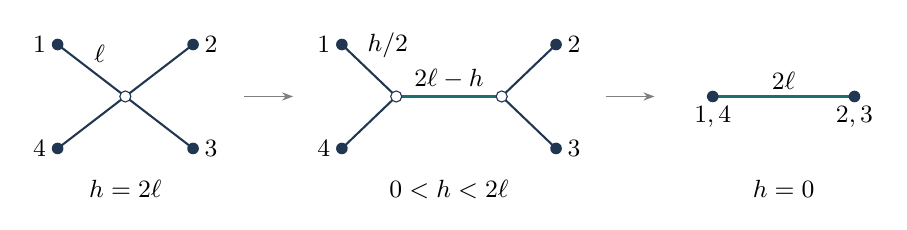
\begin{tikzpicture}[
    x=1cm,y=1cm,
    outer/.style={draw=ink,line width=.75pt},
    trunk/.style={draw=sea,line width=1.15pt},
    site/.style={circle,fill=ink,inner sep=0pt,minimum size=4.2pt},
    branch/.style={circle,draw=ink,fill=white,inner sep=0pt,minimum size=4.0pt},
    lab/.style={font=\small,inner sep=2pt},
    stage/.style={font=\small,anchor=north,inner sep=1pt}
  ]
  \begin{scope}
    \coordinate (p) at (0,0);
    \coordinate (one) at (-.86,.66);
    \coordinate (four) at (-.86,-.66);
    \coordinate (two) at (.86,.66);
    \coordinate (three) at (.86,-.66);
    \draw[outer] (one)--(p)--(two) (four)--(p)--(three);
    \node[lab,above right] at (-.47,.36) {$\ell$};
    \node[branch] at (p) {};
    \foreach \pt/\val/\side in {one/1/left,four/4/left,two/2/right,three/3/right}{
      \node[site] at (\pt) {};
      \node[lab,\side=2pt] at (\pt) {$\val$};
    }
    \node[stage] at (0,-1.02) {$h=2\ell$};
  \end{scope}
  \draw[-{Stealth[length=4pt]},draw=black!50] (1.51,0)--(2.13,0);
  \begin{scope}[shift={(4.11,0)}]
    \coordinate (leftbranch) at (-.67,0);
    \coordinate (rightbranch) at (.67,0);
    \coordinate (one) at (-1.36,.66);
    \coordinate (four) at (-1.36,-.66);
    \coordinate (two) at (1.36,.66);
    \coordinate (three) at (1.36,-.66);
    \draw[outer] (one)--(leftbranch)--(four) (two)--(rightbranch)--(three);
    \draw[trunk] (leftbranch)--(rightbranch);
    \node[lab,above] at (0,.02) {$2\ell-h$};
    \node[lab,above right] at (-1.11,.41) {$h/2$};
    \node[branch] at (leftbranch) {};
    \node[branch] at (rightbranch) {};
    \foreach \pt/\val/\side in {one/1/left,four/4/left,two/2/right,three/3/right}{
      \node[site] at (\pt) {};
      \node[lab,\side=2pt] at (\pt) {$\val$};
    }
    \node[stage] at (0,-1.02) {$0<h<2\ell$};
  \end{scope}
  \draw[-{Stealth[length=4pt]},draw=black!50] (6.10,0)--(6.72,0);
  \begin{scope}[shift={(8.36,0)}]
    \draw[trunk] (-.90,0)--(.90,0) node[lab,midway,above] {$2\ell$};
    \node[site] at (-.90,0) {};
    \node[site] at (.90,0) {};
    \node[lab,below] at (-.90,-.05) {$1,4$};
    \node[lab,below] at (.90,-.05) {$2,3$};
    \node[stage] at (0,-1.02) {$h=0$};
  \end{scope}
\end{tikzpicture}
\caption{Collision of the fourth tip with the first. On the middle
tree the distance inside each pair is \(h\), and the segment between
pair midpoints has length \(2\ell-h\). At the right endpoint the
common label is a single wire of length \(2\ell\).}
\label{fig:collision}
\end{figure}


Across these three arms the depth slopes sum to \(-1/2\) at each of
the first three sites and to \(3/2\) at site \(4\). To make all depths
harmonic, add two arms of length \(\ell\). On an unused finite arm
\(a\in F\setminus\{z_1,z_2,z_3\}\) increase every depth at slope
\(1/2\). By specialization its end rate is at most \(D_{3\ell/2}\).
On the outer arm use \(c=t^{-r}u\). Only the fourth depth changes, at
slope \(-2\). At \(r=\ell\) this site is \(P(0,-\ell)\). Write
\(D_\ell^-\) for the resulting label rate.
The ray price functions are continuous at their origins. Indeed for
small signed \(r\) the same affine depth prescriptions and \(t^r\) or
\(t^{-r}\) give a convex extension across zero.

Figure~\ref{fig:harmonic} records the five depth changes in a single
comparison. The sum down each column is zero, which is the harmonicity
condition for the corresponding site.

\begin{figure}[htb]
\centering
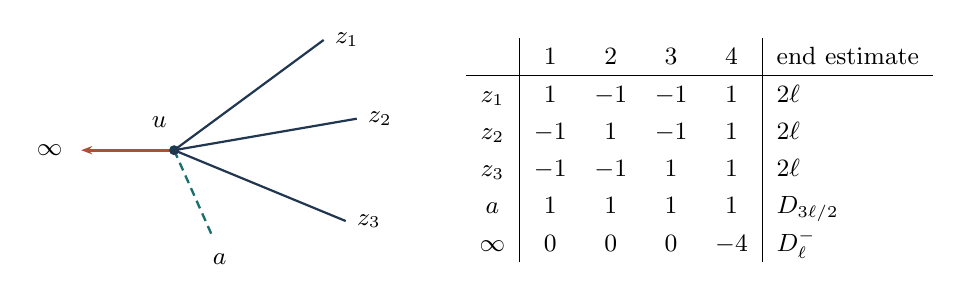
\begin{tikzpicture}[font=\small,
 inner/.style={draw=ink,line width=.8pt},
 end/.style={inner sep=2pt,anchor=west},
 twig/.style={draw=sea,densely dashed,line width=.85pt},
 up/.style={draw=rust,line width=1.05pt}]
 \draw[inner] (0,0)--(1.9,1.4) node[end] at (1.96,1.4){$z_1$};
 \draw[inner] (0,0)--(2.32,.4) node[end] at (2.38,.4){$z_2$};
 \draw[inner] (0,0)--(2.18,-.9) node[end] at (2.24,-.9){$z_3$};
 \draw[twig] (0,0)--(.48,-1.08);
 \draw[up,{Stealth[length=4pt]}-] (-1.18,0)--(0,0);
 \node at (-1.58,0) {$\infty$};
 \node at (.58,-1.38) {$a$};
 \fill[ink] (0,0) circle (1.8pt);
 \node at (-.19,.36) {$u$};
 \node[anchor=west] at (3.58,0) {$
  \renewcommand{\arraystretch}{1.22}
  \begin{array}{c | c c c c | l}
     &1&2&3&4&\text{end estimate}\\ \hline

    z_1 &1&-1&-1&1& 2\ell\\
    z_2 &-1&1&-1&1& 2\ell\\
    z_3 &-1&-1&1&1& 2\ell\\
    a&1&1&1&1& D_{3\ell/2}\\
    \infty&0&0&0&-4&D_\ell^-
  \end{array}$};
\end{tikzpicture}
\caption{The five arms based at the generic point \(u\) of the
parameter disk. The three collision arms have length \(2\ell\), the
unused finite arm \(a\) and the outer arm have length \(\ell\). The
table gives twice the four depth slopes and an upper bound for the
label rate at each end.}
\label{fig:harmonic}
\end{figure}


We compare \(D_\ell^-\) to the generic rate. Start the outer ray
at a fixed small depth \(\lambda>0\) and stop at \(0<R<\lambda\),
with all lengths rational. Write \(D(\lambda,R)\) for the rate.
The first three sites have radius \(\lambda\) about \(P(0,0)\).
By \eqref{eq:motion-tree} the fourth site also has radius \(\lambda\),
with its first \(R\) units of geodesic going toward negative depths.
Contract all four radii from \(\lambda\) to \(\ell\le R\).
This gives the placement defining \(D_\ell^-\), so convexity gives
\[
   \frac{D_\ell^-}{2\ell}\le\frac{D(\lambda,R)}{2\lambda}.
\]
Taking the upper limit in \(\ell\), then \(R\downarrow0\) by ray
continuity, then \(\lambda\downarrow0\), yields
\(\limsup D_\ell^-/(2\ell)\le \underline D\). Substituting the upper bound for
the fourth finite end into \eqref{eq:motion-star} gives
\begin{equation}\label{eq:motion-fourstar}
 0\le 3\frac{2\ell-D_\ell}{2\ell}
      +\frac{D_\ell^--D_\ell}{\ell}
      +\frac{D_{3\ell/2}-D_\ell}{\ell}.
\end{equation}
The three collision arms contribute \(3(1-\underline D)\) in the limit. The outer
arm has upper limit at most zero, and the last term tends to \(\underline D\) since
\(D_{3\ell/2}/(3\ell)\to \underline D\). Hence \(0\le 3(1-\underline D)+\underline D\), giving
\begin{equation}\label{eq:motion-upper}
                        \underline D\le 3/2 .
\end{equation}

The rectangular comparison of Section~\ref{sec:boundary} will use this
bound near the endpoint \(h=0\) in Figure~\ref{fig:collision}. There
the three fixed tips form a tripod with a pair of short arms and one
long arm. Propagating the resulting limiting price equality to the
balanced tripod gives a common-label rate of \(8/3\). The three
matrix multiplication wires on that tripod have total length \(6\),
so the rank comparison has exponent \(6/(8/3)=9/4\).

\section{A lower bound from the price of a shared label}\label{sec:boundary}

Consider a square matrix product of side \(n\), with its two inputs
and its output at the tips of a tripod with three unit arms. Each of
the three matrix indices is shared by two tips at distance \(2\), so
the product tensor has price \(6\log n\). A rank-\(r\) decomposition
supplies that tensor from a label with \(r\) values shared by all
three tips. If the rate of this shared label is \(8/3\), its price is
\((8/3)\log r\), and price monotonicity gives \(r\ge n^{9/4}\).
We will find such a tripod in the family constructed in
Section~\ref{sec:motion}. We first test the shared-label rate when one
arm is much longer than the other two. The following principle carries
the resulting equality to three equal arms.

\begin{proposition}[Tripod principle]\label{prop:tripod}
Over an algebraically closed field, place three sites at pairwise
distances \(a_i+a_j\) for \(i\ne j\), where \(a_1,a_2,a_3\ge0\).
Their common-label rate \(D(a)\) satisfies
\[
       D(a)\ \ge\ D_*(a)
       :=a_1+a_2+a_3-\bigl(a_1^{-1}+a_2^{-1}+a_3^{-1}\bigr)^{-1}.
\]
The reciprocal term is zero when any \(a_i=0\).

Now fix three infinite rays in a spectral space that form a metric
tripod with origin \(O\), and suppose that their prices are
homogeneous under radial dilation. In \(D(a)\), place site \(i\) on
ray \(i\) at distance \(a_i\) from \(O\). If \(D(a)-D_*(a)\)
vanishes at one positive triple, it vanishes at every positive
triple. The same conclusion holds if the defect tends to zero as one
arm tends to infinity with the other two held at fixed positive lengths.
\end{proposition}

The first assertion applies to any placement with the specified
distances. The second compares placements on a single tripod.
Sections~\ref{sec:profiles}--\ref{sec:contact} prove both assertions by
studying how the price of polynomial multiplication changes with its
degree and with the positions of its coefficients.

\subsection{A decoder for rectangular multiplication}

Multiply an \(s\times q\) matrix by a \(q\times s\) matrix over the
algebraically closed field \(F\) of Section~\ref{sec:motion}, taking
\(s=N^{1/2}\) and \(q=N^{1/4}\) for a fourth power \(N\). The product
has \(N\) entries. Place its output at \(A\) and its inputs at
\(C,D'\), with respective arm lengths \(c,a,b\). The outer indices
give wires of size \(s\) on \(AC,AD'\), and the inner index gives a wire
of size \(q\) on \(CD'\). The price of the product, divided by
\(\log N\), therefore satisfies
\[
   c+\tfrac34(a+b)
   \ \le\ c+a+b-\frac{ab}{a+b}
   \ \le\ D_*(c,a,b)\ \le\ D(c,a,b).
\]
Here \(ab/(a+b)=0\) if \(a=b=0\). This gives the rectangular bound
associated with half-width multiplication \cite{uznanski,abvz}.

In particular, for every \(\eta>0\) there are arbitrarily large
such \(N\) for which the exact tensor rank is at most \(N^{1+\eta}\).
Indeed, start with a sufficiently large fourth power \(N_0\)
and a full diagonal of size \(\lceil N_0^{1+\eta/2}\rceil\).
The displayed inequality at every spectral point gives strict
spectral comparison with this diagonal. Each tensor power of the product
is a restriction of a bounded number of copies of the corresponding
power of the diagonal. At sufficiently large powers the exponent
\(1+\eta\) absorbs both this multiplicity and the rounding.

\begin{lemma}[A decoder with short rows]\label{lem:secondary}
For every \(\epsilon>0\) there is a \(\delta>0\) such that for
unbounded fourth powers \(N\) the \(N\) output bilinear forms \(B_e\)
of this product admit decompositions
\[
    B_e=S_e+R_e,\qquad
    \operatorname{rank}S_e\le N^\epsilon,\qquad
    \dim\langle R_e:1\le e\le N\rangle\le N^{1-\delta}.
\]
\end{lemma}

The two bounds have different uses. A short sum of simple products
computes each \(S_e\) once the output index \(e\) is shared.
The corrections \(R_e\) may be expensive individually, but their
entire span can be sent across a single wire. To obtain the bounds
uniformly in the base format, we implement a tensor power of a decoder
using one work register. For related nonrigidity estimates for
Kronecker products, see \cite{almanrigidity,kivva}.

\begin{proof}
It suffices to take \(0<\epsilon<1\). Fix an integer \(K>10/\epsilon\).
For a base format with \(d\) output entries and rank
\(d\le r\le d^{1+\eta}\), let \(M\) be the \(d\times r\) matrix that
expresses its outputs in terms of \(r\) simple bilinear products.
We will choose \(\eta\) below. The \(Km\)-th tensor power has
\(N=d^{Km}\) entries. Pad each decoder block \(M^{\otimes m}\) with
zero rows and columns to side \(2^t\), where \(t=\lceil m\log_2 r\rceil\).
The full padded decoder has side \(T=2^{Kt}\). An index consists of
\(K\) registers of \(t\) bits each.

Apply the first block matrix to the first register. For each subsequent
block, swap its register with the first, apply the block matrix there,
and swap back. An exchange of registers performs \(t\) simultaneous
exchanges of pairs of bits. A bit exchange transposes two of four
letters, \(01\) and \(10\). Its matrix factors into a fixed number of
elementary shears and diagonal signs, over any field. Thus a register
exchange consists of a fixed number of stages, each applying the same
local shear or diagonal sign at every bit position.

For a shear, let the high letter be the target of its off-diagonal
entry. Immediately before and after the stage, project onto the
coordinates whose register pair contains between \(t/4-\rho t\) and
\(t/4+\rho t\) high letters, for a fixed small \(\rho>0\).
The discarded fraction of coordinates is at most \(e^{-c_\rho t}\)
for large \(t\), by the binomial tail. Telescoping over the \(O(K)\)
projections bounds the rank of the discarded part of the decoder by
\(O(K)Te^{-c_\rho t}\le T^{1-\gamma}\), with \(\gamma=\gamma(K,\rho)>0\).
On a path retained at a shear stage, every change creates a high
letter, so at most \(2\rho t\) positions change.

Only the first register is acted on by a block matrix. Every other
register participates in just two exchanges, so its input lies within
Hamming distance \(C\rho t\) of its output on a retained path, for an
absolute constant \(C\). Each output row of the retained decoder
therefore has at most
\[
       2^t\left(\sum_{j\le C\rho t}\binom{t}{j}\right)^{K-1}
       \ \le\ T^{1/K+o_{\rho\downarrow0}(1)}
\]
nonzero entries. Choose \(\rho\) so that this exponent is below
\(\epsilon/2\), then choose \(\eta\) sufficiently small. Since
\(T\le 2^K N^{1+\eta}\), for all large \(m\) the two bounds become
\(N^\epsilon\) entries per retained row and rank \(N^{1-\delta}\)
for the discarded matrix, with \(\delta=\gamma/2\). Remove the
zero padding and apply both matrices to the list of simple bilinear
products. The retained rows give the forms \(S_e\), and the image of
the discarded row space spans the \(R_e\).
\end{proof}

\subsection{Two copies of the output near a collision}

Choose the collision in Section~\ref{sec:motion} where site \(4\)
approaches site \(3\), and denote sites \(1,2,3,4\) by \(A,B,C,D'\).
At parameter \(r\) write \(L=2\ell\) and \(h=L-r\), with \(0<h<L\).
The distances within \(AB\) and \(CD'\) are both \(h\), and all four
cross distances are \(L\). Write \(D_\ell(h)\) for the four-site
common-label rate. At the collision \(D_\ell(0)=L\), and at the
generic four-site placement \(D_\ell(L)=D_\ell\). Convexity gives
\[
                   D_\ell(h)\le L+\frac hL(D_\ell-L).
\]

Duplicate the output index \(e=(i,i')\) of the rectangular product at
\(A\) and \(B\), leaving its two inputs at \(C,D'\). The resulting tensor is
\[
 U_N=\sum_e e_e\otimes e_e\otimes B_e
     =\sum_{\substack{1\le i,i'\le s\\1\le j\le q}}
        e_{ii'}\otimes e_{ii'}\otimes e_{ij}\otimes e_{ji'} .
\]
The index \(i\) is a shared label at \(A,B,C\), the index \(i'\) is a
shared label at \(A,B,D'\), and \(j\) travels on the short wire \(CD'\).
Writing \(D_{ABC},D_{ABD'}\) for the two triple rates, we have
\[
   \frac{H(U_N)}{\log N}=\frac{D_{ABC}+D_{ABD'}}2+\frac h4 .
\]
Both triples have arms \((h/2,h/2,L-h/2)\). Their reciprocal
correction in Proposition~\ref{prop:tripod} is at most \(h/4\), so
both rates are at least \(L+h/4\).

Use the decomposition \(B_e=S_e+R_e\) from Lemma~\ref{lem:secondary}.
In units of \(\log N\), the tensor formed from the \(S_e\) costs at
most \(D_\ell(h)+\epsilon h\). Share the label \(e\) at all four sites,
then use a wire of size at most \(N^\epsilon\) on \(CD'\) to supply
the simple products for the specified \(e\). The tensor formed from
the \(R_e\) has matrix rank at most \(N^{1-\delta}\) across the cut
\(AB\mid CD'\). A wire between \(A\) and \(C\) supplies this rank, and
wires within the two pairs deliver the legs at \(B\) and \(D'\), each
of dimension at most \(N\). This costs at most \((1-\delta)L+2h\).

Take \(h/L<\delta/2\). The correction then costs less than \(L\), and
\(D_\ell(h)\ge L\) by restriction to a cross pair. For a fixed placement
the ordinary-sum price bound costs an additive constant independent of
\(N\). Sending \(N\) to infinity along the formats of Lemma~\ref{lem:secondary} and
then using Equation~\eqref{eq:motion-upper} at fixed \(h/L\) gives
\[
  \frac{D_{ABC}+D_{ABD'}}2+\frac h4
  \ \le\ D_\ell(h)+\epsilon h
  \ \le\ L+\bigl(\tfrac12+\epsilon+o_{\ell\downarrow0}(1)\bigr)h .
\]
Subtract the lower bound \(D_{ABD'}\ge L+h/4\) to obtain
\[
        D_{ABC}\le L+h/4+\bigl(2\epsilon+o_{\ell\downarrow0}(1)\bigr)h.
\]

The first three sites lie on the fixed rays \(z_1,z_2,z_3\) out of
the depth-zero point. Take the tangent tripod there by placing sites
at depths \(t a_i\), dividing prices by \(t\), and letting \(t\downarrow0\)
in a spectral ultralimit. On these fixed rays the rescaled price of
every nonzero tensor has a limit, since its original price is convex
in \(t\) and vanishes at zero. The limiting prices are homogeneous
under radial dilation.

Set \(t=h/2\) and hold \(b=2L/h-1\) fixed. The three depths become
\(t(1,1,b)\). Dividing the last inequality by \(t\) gives
\(D(1,1,b)\le b+3/2+4\epsilon\), whereas
\[
             D_*(1,1,b)=b+\tfrac32+\frac{1}{4b+2}.
\]
Thus \(0\le D(1,1,b)-D_*(1,1,b)\le4\epsilon\) for every sufficiently
large rational \(b\), and for real \(b\) by continuity. Sending \(b\)
to infinity and then \(\epsilon\) to zero gives contact at infinity
on this fixed tripod. Proposition~\ref{prop:tripod} now gives
\(D(1,1,1)=3-1/3=8/3\). The three-wire price comparison at the start
of this section yields \(r\ge n^{9/4}\), proving Theorem~\ref{thm:motion}.

\section{Polynomial multiplication near contact}\label{sec:profiles}

The tripod principle compares the price $D$ of a common label at the
three terminals with the lower bound $D_*(a)=\sum_i a_i-(\sum_i a_i^{-1})^{-1}$
for their arm lengths $a_i>0$. We call equality \emph{contact} and write
$\Delta=D-D_*(a)$ for the defect. To propagate contact to other triples
of arm lengths, we need to know how a price changes when just one input
width varies. Polynomial multiplication supplies a tensor for which we
can measure this change. Its price as one input grows has a limiting slope
and intercept after exponentiation. Proposition~\ref{thm:profile-rigidity}
determines the intercepts to within $O(\Delta)$. Section~\ref{sec:energy}
then compares different placements, and Section~\ref{sec:contact} uses the
comparison to propagate equality.

Throughout these three sections the field is algebraically closed and
prices use natural logarithms with the distances held fixed. A label
with $q$ values shared at the terminals costs $D\log q$. On an embedded
tripod, including its origin gives the same price. A duplicate at either
of two terminals is free, and convexity bounds its cost at every point
on the geodesic between them.

\subsection{The continuum profile}
Place a finite nonempty set of inputs and one output in a spectral space.
Write $H$ for price and $D>0$ for the common-label rate of the placement.
For integer lengths $L_i\ge1$, let $M(L)$ multiply univariate polynomials
of degrees less than $L_i$, retaining all output coefficients. The following
normalization also fixes the constant in the energy formula below.

\begin{lemma}\label{lem:continuum-profile}
There is a continuous coordinatewise nondecreasing function $P$ on the positive
orthant such that, if $L_i/N\to t_i>0$, then
\[
 H(M(L))=D\log N+P(t)+o(1),\qquad P(ct)=P(t)+D\log c.
\]
For polynomials in $m$ variables with total input degrees at most
$\lfloor Nt_i\rfloor$, the corresponding price is
$mD\log N+mP(t)-D\log(m!)+o(1)$ for each fixed $m$.
\end{lemma}

\begin{proof}
Evaluation and interpolation bound $H(M(L))$ by $D\log(\sum_iL_i)$.
In the other direction, $M(kL)$ degenerates to $k$ direct copies of
$M(L)$. Indeed, divide $[0,1]$ into $k$ equal intervals and choose a
continuous convex piecewise affine function with a strict change of slope
at each division. An input monomial of degree $d_i$ has normalized position
$(d_i+1/2)/(kL_i)$. Give it weight $kL_i$ times the function there. Give the
output the opposite weight at the weighted mean of those positions, with
coefficient $k\sum_i L_i$. The output weight depends only on the sum of
degrees. Jensen's inequality retains precisely the terms whose inputs lie
in one interval. Different intervals use disjoint input and output
coordinates, and each surviving block is a translated copy of $M(L)$.
The weight equalities define a rational linear subspace. Rational
approximation within it preserves the finitely many strict inequalities,
and scaling gives integral weights. Rescaling the coordinates and using
closedness of price sublevels therefore gives the asserted degeneration.

For $L_i=\lfloor Nt_i\rfloor$ the normalized cost at $N$ therefore
dominates that at any fixed sufficiently large $M$, up to
$D\log(M\lfloor N/M\rfloor/N)$. Taking first the lower limit in $N$ and
then the upper limit in $M$ proves convergence. Changing the unit of $N$
gives log homogeneity, first with floors by squeezing the scales and then
for real $N$. Coordinate monotonicity and squeezing between
$(1\pm\epsilon)t$ give continuity and allow $o(N)$ errors in the lengths.

For the assertion about total degree, divide the exponent vector at
input $i$ by $Nt_i$ and at the output by $N\sum_i t_i$. All inputs now
range over lattice points in the unit simplex. To cut this domain by a
hyperplane, first discard input points on the plane. Apply the same
convex weighting as above, using the positive part of the defining
affine form and coefficients $Nt_i$. Jensen's inequality retains terms
whose inputs are on the same side. Their outputs are on that side as
well, so the two blocks form a direct sum. One may repeat the cut within
each block.

On a translated axis-parallel cube of side $s$, multiplication factors
over the $m$ coordinates. The univariate limit shows that its
exponentiated price, divided by $N^m\exp(mP(t)/D)$, tends to its volume
$s^m$. Translation just relabels exponents and rounding a cube side
changes widths by $O(1)$. Packing the simplex with interior grid cubes
thus bounds its normalized price from below by $1/m!$, since
$\exp(H/D)$ adds on direct sums. For the upper bound, start with an
enclosing cube and cut off a slightly enlarged simplex, so all input
points of the desired tensor survive in one cell. Pack the complementary
cells with interior grid cubes. The enclosing tensor dominates the
direct sum of the desired tensor and all packed cubes. Refining the
grid and shrinking the enlargement accounts for the whole complementary
volume and gives the matching upper bound $1/m!$. Taking logarithms
proves the formula.
\end{proof}

\subsection{A label visible at two sites}

We also need a lower bound for a sum whose block label is visible at
only two of three sites. Suppose $T=\sum_b T_b$ with $T_b\ne0$ and
$T_b\in X\otimes Y_b\otimes Z_b$, where the $Y_b$ are direct subspaces
at $Y$, and the $Z_b$ are direct subspaces at $Z$. For every probability
law $q$ on the block labels, writing
$\operatorname{Ent}(q)=-\sum_b q_b\log q_b$, we have
\begin{equation}
 H(T)\ge\sum_b q_b H(T_b)+d(Y,Z)\operatorname{Ent}(q).
 \label{eq:pair-entropy}
\end{equation}
To see the entropy term, take a rational $q$ and a power $n$ for which
each $nq_b$ is integral. At $Y$ and $Z$, retain the
$M=n!/\prod_b(nq_b)!$ words of type $q$. Each word has price
$n\sum_bq_bH(T_b)$. The shared-leg separation of~\cite[Proposition~3.1]{nine},
in the interpolation form of~\cite[Proposition~2.1]{lu}, degenerates
$2M-1$ direct copies of the retained tensor to the full direct sum of
the $M$ word blocks, each tensored with an $M$-dimensional wire on
$Y,Z$. Interpolation uses $2M-1$ distinct field elements, available
in every algebraically closed field. Comparing the two prices gives
\[
 nH(T)+D\log(2M-1)\ \ge\
 n\sum_bq_bH(T_b)+(D+d(Y,Z))\log M ,
\]
where $D$ is the common-label rate of the three sites.
Now $\log((2M-1)/M)\le\log2$ and $n^{-1}\log M\to\operatorname{Ent}(q)$.
Division by $n$ and continuity in $q$ give~\eqref{eq:pair-entropy}.

\subsection{Slopes and intercepts on a triangle}

Use $i,j,k$ for the three sites in any order and suppose their arms $a_i$
are positive. Put $d_i=d(j,k)=a_j+a_k$, $D=\delta(\{i,j,k\})$, and
write $P_k(x,y)$ for the profile with output $k$ and input widths $x$ at
$i$ and $y$ at $j$. We identify each argument by its site.
For a fixed first input define
\[
 F_{ik}(t)=\exp\bigl(P_k(t_i=1,t_j=t)/d_i\bigr).
\]
The determinant filtration and the shifted three-block degeneration for
polynomial multiplication \cite[proofs of Lemmas~4.1 and~4.2]{nine} give
\[
 F_{ik}\text{ is concave},\qquad
 F_{ik}(3t+1)\ge 2F_{ik}(t)+F_{ij}(t).
\]
In the first degeneration a two-dimensional wire on $j,k$ supplies two
blocks, with the length at $j$ increased and decreased by one. The blocks
are direct on that pair. Optimizing the pair-label inequality over the
block probabilities adds their exponentiated prices at scale $d_i$.
This gives midpoint concavity on the lattice of lengths, hence concavity
in the limit. In the second degeneration the longer length is
$3L_j+L_i-1$, and one of the three blocks exchanges $j$ and $k$. The same
pair-label inequality and Lemma~\ref{lem:continuum-profile} give the second
displayed assertion. Both degenerations work in every characteristic.
For the first, injectivity of multiplication by the determinant and
a dimension count give the degree-one Clebsch--Gordan determinant
sequence (see~\cite{kowalski}). Lifting monomials to its filtration
suffices. The second uses a monomial grading, and reversal of the order
on a leg identifies the middle block.

Positive increasing concave functions have finite limiting slopes at
infinity. Dividing the three-block inequalities by $t$ shows that the
slopes of $F_{ik}$ and $F_{ij}$ are equal. For $S=F_{ik}+F_{ij}$ we have
$S(3t+1)\ge3S(t)$. Iterating along
$t_n=3^n(t+1/2)-1/2$ gives
$S(t)/(t+1/2)\le \lim_{n\to\infty}S(t_n)/(t_n+1/2)$, twice the common slope. In particular the common slope is positive. Write it as
$\exp(c_i/d_i)$.
For either function the excess over the line through zero of that slope
is nonnegative and increasing. The bound on $S$ therefore gives numbers
$\beta_{ik},\beta_{ij}\ge0$, with $\beta_{ik}+\beta_{ij}\le1$, such that
\[
 t\le e^{-c_i/d_i}F_{ik}(t)\le t+\beta_{ik}.
\]
Here $\beta_{ik}$ is the limiting excess after division by the slope.
In particular $P_k$ is $d_i$-Lipschitz as a function of $\log y$ with $x$
fixed, since every one-sided derivative of $F_{ik}$ lies between zero and
$F_{ik}(t)/t$.

Set $h=(\sum_i1/a_i)^{-1}$, $b_i=a_i-h$, $u_i=b_i/a_i$,
$\beta_{ik}^*=a_k/d_i$, and $\Delta=D-D_*(a)$, where
$D_*(a)=\sum_i a_i-h$. Since $P_k(x,y)=D\log x+P_k(1,y/x)$
and $D-d_i=b_i+\Delta$, the intercept bound gives an upper envelope
valid at every pair of widths,
\begin{equation}\label{eq:profile-upper}
 P_k(x,y)\le U_{ik}(x,y):=c_i+(b_i+\Delta)\log x+d_i\log(y+\beta_{ik}x).
\end{equation}

\begin{proposition}[Profile near contact]\label{thm:profile-rigidity}
We have $\Delta\ge0$. If $\min_i u_i\ge\eta>0$, there is a number $C$
common to all three sites such that
\begin{equation}\label{eq:src2}
 d_i(\beta_{ik}-\beta_{ik}^*)=O_\eta(\Delta),\qquad
 c_i+b_i\log u_i=C+O_\eta(\Delta).
\end{equation}
In the sector $y/x\ge u_j/u_i$,
\begin{equation}\label{eq:src3}
 0\le U_{ik}(x,y)-P_k(x,y)\le O_\eta(\Delta).
\end{equation}
\end{proposition}

\begin{proof}
Let $E_{ik}=U_{ik}-P_k$ and $z_{ik}=d_i(\beta_{ik}-\beta^*_{ik})$.
Differentiating with respect to $y$ and bounding the derivative of
$F_{ik}$ below by its limiting slope yields
\[
 \partial_y P_k(x,y)\ \ge \frac{d_i}{y+\beta_{ik}x}\exp(E_{ik}(x,y)/d_i).
\]
There is a second bound from interchanging $i,j$. At differentiability
points, $x\partial_xP_k+y\partial_yP_k=D$. The profiles are locally
Lipschitz, so continuity gives the sum of the two derivative bounds at
$(x,y)=(u_i,u_j)$ even if a derivative fails to exist there.
At this point $u_j+u_i\beta^*_{ik}=1$ and $u_jd_i+u_id_j=D_*$.
Use $(1+r)^{-1}=1-r+r^2/(1+r)$ with
$r=u_i z_{ik}/d_i$, and $e^s\ge1+s$ for $s\ge0$.
Since $\eta\le u_j+u_i\beta_{ik}\le2$, this gives, for some $c_\eta>0$,
\[
 \frac{\Delta}{u_iu_j}\ge -(z_{ik}+z_{jk})+
 c_\eta\left(E_{ik}+E_{jk}
           +\frac{z_{ik}^2}{d_i}+\frac{z_{jk}^2}{d_j}\right),
\]
where all the gaps are evaluated at the specified widths.
The row sums $z_{ik}+z_{ij}$ are nonpositive since
$\beta^*_{ik}+\beta^*_{ij}=1$. Summing over output sites $k$ gives
$\Delta\ge0$ and bounds each nonnegative remainder by $O_\eta(\Delta)$.
Each row sum thus lies between $-O_\eta(\Delta)$ and zero. Each
column sum is at least $-O_\eta(\Delta)$ by the displayed inequality.
Since the columns have the same total as the rows, each column sum is
also at most $O_\eta(\Delta)$.

Comparing the two envelopes for $P_k(u_i,u_j)$ now gives
\[
 c_i+b_i\log u_i+u_i z_{ik}
 =c_j+b_j\log u_j+u_j z_{jk}+O_\eta(\Delta).
\]
Here the logarithmic Taylor remainders are controlled by
$z_{ik}^2/d_i$ and $z_{jk}^2/d_j$. The row and column estimates
show that, up to $O_\eta(\Delta)$, the entries
$(z_{12},z_{13},z_{23},z_{21},z_{31},z_{32})$ alternate between
$z_{12}$ and $-z_{12}$. Sum the three comparisons of envelopes for
$(i,j)=(1,2),(2,3),(3,1)$. The terms $c_i+b_i\log u_i$ cancel, leaving
$2(u_1+u_2+u_3)z_{12}=O_\eta(\Delta)$.
This proves \eqref{eq:src2}. The gap $E_{ik}$ depends only on $y/x$. The
difference between $t+\beta_{ik}$ and $e^{-c_i/d_i}F_{ik}(t)$ decreases
with $t$, and the latter function increases. Their log ratio hence
decreases, which proves \eqref{eq:src3}.
\end{proof}

For example, at contact on the unit tripod the predicted intercept
is $\beta^*_{ik}=1/2$ and $u_i=u_j=2/3$. Thus
$e^{-c_i/d_i}F_{ik}(t)=t+1/2$ for $t\ge1$. More generally,
\eqref{eq:src2} remains uniform as a single arm tends to infinity
while the other two stay in a compact subset of $(0,\infty)$.
If an arm has length zero, $D\ge D_*(a)$ follows from the diameter bound.

\section{Energy and radial contraction}\label{sec:energy}

Fix an output and a nonempty finite set $A$ of inputs with common-label
rate $D>0$ on all the terminals. For costs $\ell_i>0$ per unit of input
width, define the energy
\begin{equation}\label{eq:energy-widths}
 Q_A(\ell)=D+\sup_{t_i>0}\bigl(P(t)-\ell\cdot t\bigr).
\end{equation}
It is finite by the evaluation bound, convex in $\ell$, and satisfies
$Q_A(c\ell)=Q_A(\ell)-D\log c$ by log homogeneity of $P$.
A common surcharge $s$ penalizes a candidate width vector by
$s\sum_i t_i$. Hence the slope of the optimized energy along a common
cost increase measures total width. We will use the finite difference
$Q_A(\ell)-Q_A(\ell+s\mathbf1)$.
Lemma~\ref{lem:energy-compare} shows that this drop can only decrease
when inputs move towards the output and their respective costs decrease
in proportion. We prove the comparison first for homogeneous degrees,
where we can move an input between two polynomial multiplications,
and then recover $Q_A$ by rescaling those degrees.

To compare different placements, first charge a cost $f_i>0$ per
degree of a homogeneous polynomial.
Write $M_m^{\mathrm{hom}}(r)$ for multiplication of homogeneous
polynomials in $m$ variables, with input degrees $r=(r_i)_{i\in A}$.
Define
\[
 B_A(f)=\sup_{m\ge1,\ r_i\in\mathbb Z_{\ge0}}
 \frac{H(M_m^{\mathrm{hom}}(r))-\sum_i f_i r_i}{m}.
\]
This is finite. Evaluation and interpolation at a basis of evaluation
functionals on the output give rank at most its dimension. With
$R=\sum_i r_i$ and $q=\exp(-\min_i f_i/D)$, the exponential of the
cost-subtracted price at scale $D$ is bounded by
$\binom{m-1+R}{R}q^R\le(1-q)^{-m}$. The supremum is unchanged if $m$
is required to be a multiple of a prescribed integer. Indeed, using
disjoint groups of variables recovers any power of the original tensor
as a restriction of multiplication with the combined degrees.

\begin{lemma}[Adding an input]\label{lem:increasing-returns}
If $\varnothing\ne A'\subseteq A$ and $s>0$, then
\begin{equation}\label{eq:src5}
 B_A(f)-B_A(f+s\mathbf1)\ge
 B_{A'}(f)-B_{A'}(f+s\mathbf1),
\end{equation}
with costs restricted to the indicated input set. If all sites in a
restricted placement coincide, its energy is zero.
\end{lemma}

\begin{proof}
It suffices to add a single input $e$. Rewrite the claim with
$B_{A'}(f)+B_A(f+s\mathbf1)$ on the right, and choose two multiplications
approaching those suprema. They can use the same number $m$ of variables
by taking powers in separate groups. Name their variables respectively
$u=(u_1,\ldots,u_m)$ and $v=(v_1,\ldots,v_m)$. At each common input the
tensor product of the two multiplications accepts a bihomogeneous
polynomial in $(u,v)$ of prescribed bidegree. At $e$ it accepts a
polynomial $h(v)$ of degree $q$. Write $(U,V)$ for the total bidegree,
including $q$.

We realize this tensor product by a sum of multiplications in which $e$
belongs instead to the $u$ group. Rename $h(v)$ to $h(u)$ and substitute
$u-v$ for $u$ at the common inputs. Multiply, substitute $u+v$ for $u$
on the output, and project onto bidegree $(U,V)$. The substitutions on
the common inputs cancel, and the only term of $h(u+v)$ that survives
the projection is $h(v)$. This identity uses no division. Expand the
intermediate inputs into bidegrees before multiplying. If a total of $k$
degrees from the common inputs move from $u$ to $v$, the intermediate
$v$-degree is $V-q+k$. The final substitution can only increase this
degree, so a surviving sector has $k\le q$. The total degree at each
input is preserved. Thus the base cost of every sector is unchanged and
its surcharge on $v$ is at most $sV$. Each sector factors through a
multiplication on $u$ with all inputs and one on $v$ with inputs $A'$,
with local pre- and postprocessing.

Apply this construction to powers in $nm$ variables per group with all
degrees multiplied by $n$. There are polynomially many bidegree sectors
as functions of $n$, since $A$ is fixed. The price bound for an ordinary
sum costs only $O(\log n)$ beyond the largest sector price. After division
by $nm$ and passage to the limit, the right side is bounded by
$B_A(f)+B_{A'}(f+s\mathbf1)$, as claimed.
\end{proof}

\subsection{From degrees to widths}

Charging $\ell_i/N$ per degree makes degrees of order $N$ correspond
to widths of order one. The factor $1/m!$ for total-degree polynomials
in Lemma~\ref{lem:continuum-profile} accounts for the additive $D$ in
\eqref{eq:energy-widths}.

\begin{lemma}[Continuum limit of the degree energy]\label{lem:continuum-energy}
At a placement with common-label rate $D>0$, one has
\begin{equation}\label{eq:src6}
 B_A(\ell/N)=D\log N+Q_A(\ell)+o(1)
 \qquad(N\longrightarrow\infty).
\end{equation}
\end{lemma}

\begin{proof}
Write $S_m(r)$ for polynomial multiplication with total degree
\emph{at most} $r_i$ on each input. Its price minus degree costs, divided
by $m$, is a lower bound on $B_A$. Indeed, $n$ copies on disjoint variable
groups restrict from homogeneous multiplication with $nm+1$ variables
and degrees $nr_i$. Use the last variable to homogenize and set it to one
on the output. Hence
$B_A(f)\ge n(H(S_m(r))-f\cdot r)/(nm+1)$, and we let $n\to\infty$.
For $r_i=\lfloor Nm t_i\rfloor$, Lemma~\ref{lem:continuum-profile} now gives
\[
 \liminf_{N\to\infty}(B_A(\ell/N)-D\log N)
 \ge P(t)-\ell\cdot t+D\bigl(\log m-m^{-1}\log(m!)\bigr).
\]
The last summand tends to $D$. Taking the supremum over $t$ gives the
required lower bound.

For the upper bound take integer $N$. In the supremum defining $B_A$
we may use $Km$ variables grouped into $K$ sets of size $m$. At each
input, record the total degree in each group by its bin
$[(b_i-1)N,b_iN)$, $b_i\ge1$. Within a fixed bin pattern the
multiplication restricts from the product of $S_m(Nb)$ over the groups,
and the cost in each group is at least $\sum_i\ell_i(b_i-1)$. The price
of the sum over patterns is bounded by the logarithm of the sum of their
exponentiated prices at scale $D$. Summing over all bins independently
in each group enlarges this last sum to a $K$th power. Dividing its
logarithm by $Km$ and taking the supremum gives
\[
 B_A(\ell/N)\le \frac Dm\log\sum_{b\in\mathbb Z_{>0}^A}
 \exp\left(\frac{H(S_m(Nb))-\sum_i\ell_i(b_i-1)}{D}\right).
\]
For fixed $m$, after removing $N^m$ from the sum, the terms are dominated
by a constant times $(m+\sum b_i)^m\exp(-\ell\cdot b/D)$, by the
output-dimension bound. Lemma~\ref{lem:continuum-profile} and dominated
convergence bound the upper limit of $B_A(\ell/N)-D\log N$ by
\[
 D\left(\log m-\frac{\log(m!)}m\right)
 +\frac{\sum_i\ell_i}m+
 \frac Dm\log\sum_b\exp\left(\frac{mP(b/m)-\ell\cdot b}{D}\right).
\]
For $0<\epsilon<1$, use the supremum of
$P(t)-(1-\epsilon)\ell\cdot t$ to bound the last term, with a remainder
at most $(D/m)\log\sum_b\exp(-\epsilon\ell\cdot b/D)$.
Let $m\to\infty$, then $\epsilon\downarrow0$, using the scaling relation
for $Q_A$. Monotonicity in $N$ gives the same limit at real scales.
\end{proof}

\begin{lemma}[Radial contraction]\label{lem:energy-compare}
Move each input $i$ towards the output along its geodesic, to a fraction
$0<\lambda_i\le1$ of its original distance. Write $A'$ for the resulting
placement and $\ell'_i=\lambda_i\ell_i$. For $s>0$ one has
\begin{equation}\label{eq:src7}
 Q_A(\ell)-Q_A(\ell+s\mathbf1)\ge
 Q_{A'}(\ell')-Q_{A'}(\ell'+s\mathbf1)
\end{equation}
when both placements have positive common-label rate.
\end{lemma}

\begin{proof}
Duplicating an input at its own site and cost leaves $B$ unchanged, by
local multiplication. An additional input at the output at zero cost
also leaves $B$ unchanged, by local multiplication on the output.
The reverse inequalities in both statements use degree zero at the
added input. For each fixed multidegree the price is convex as the
added input moves on a geodesic, and the subtracted cost is affine.
Thus an added input at radial fraction $\lambda_i$ and cost at least
$\lambda_i f_i$ leaves $B$ unchanged, first for one addition and then
for all of them. This applies both at $f=\ell/N$ and after increasing
every cost by $s/N$, since $\lambda_i\ell_i+s\ge
\lambda_i(\ell_i+s)$. Insert the moved inputs at their specified costs
and use Lemma~\ref{lem:increasing-returns} to delete the original
inputs. The energy drop for the resulting placement is bounded by the
drop for the original one. Let $N\to\infty$ in \eqref{eq:src6}. The
leading $D\log N$ cancels separately at each placement, which proves
\eqref{eq:src7}.
\end{proof}

\section{Propagation of equality on a tripod}\label{sec:contact}

Fix three infinite rays forming a metric tripod with origin $O$.
Prices on these rays are homogeneous under simultaneous radial
dilation. Proposition~\ref{thm:profile-rigidity} gives
$D(a)\ge D_*(a)$ at the three tips of lengths $a_1,a_2,a_3$.
We now prove the rigidity assertion of Proposition~\ref{prop:tripod}.
Equality at a single triple of lengths forces equality at every
triple. The same conclusion follows from equality approached along
one arm as its length tends to infinity with the other two lengths
fixed and positive.

Use the reciprocal lengths
\[
 v_i=1/a_i,\qquad h(a)=\frac{1}{v_1+v_2+v_3},\qquad
 \Delta(v)=D(a)-D_*(a).
\]
An infinitely long arm now corresponds to a coordinate face.
The proof first compares integrals of the defect along the three
coordinate rays out of $v$. At a zero of $\Delta$ these integrals
agree. Radial homogeneity then forces their common value to vanish.

\subsection{Comparing the three directional integrals}

The profile lower bound and the spanning tree through $O$ give
$D_*(a)\le D(a)\le\sum_i a_i$. Equivalently,
\begin{equation}\label{eq:defectbound}
 0\le \Delta(v)\le\frac{1}{v_1+v_2+v_3},\qquad
 \Delta(rv)=r^{-1}\Delta(v)\quad(r>0).
\end{equation}
On the positive octant $\Delta$ is locally Lipschitz and locally
semiconvex. The latter means that adding $C|v|^2$ makes it convex
on a given small ball for a suitable $C$. Indeed, $D$ is convex in
the arm lengths by joint geodesic convexity. Transport of a single
tip through distance $t$ changes $D$ by at most $t$. The change of
variables $a_i=1/v_i$ has bounded first and second derivatives on
interior compact sets, and $D_*$ is smooth there.

As $v_1\downarrow0$, the function $D(a)-\sum_i a_i$ is
nonincreasing by the same transport bound, and is bounded below by
$-h(a)$. Since $h(a)$ also has a limit there, $\Delta$ extends to the open face $v_1=0$.
The Lipschitz and semiconvexity constants in the other two variables
are uniform when those variables range in compact subsets of
$(0,\infty)$, including as $v_1\downarrow0$. Thus the extension is
continuous and has the same tangential regularity. The other faces
are treated by relabeling.

For each interior $v$ and coordinate vector $e_i$, set
\[
 J_i(v)=\int_0^\infty
 \left[\Delta(v+t e_i)-\mathbf 1_{\{t\le1\}}\Delta(v)\right]
       \frac{dt}{t}.
\]
The subtraction makes the integral convergent at zero by local
Lipschitz continuity. Equation~\eqref{eq:defectbound} gives
convergence at infinity. We will prove the estimate
\begin{equation}\label{eq:src10}
                   |J_i(v)-J_j(v)|\le C\Delta(v).
\end{equation}
Here $C$ is locally uniform up to each open face. On a face the same
estimate holds for its two tangential directions.

\paragraph{An energy derivative.}
Keep $v$ fixed and use $a_i=1/v_i$ as the locations of three input
tips, with the output at $O$. Let $Q$ be their energy from
Equation~\eqref{eq:energy-widths}. For a variable
$s\in(0,\infty)^3$, put
\[
 G_v(s)=Q\big((a_i s_i)_i\big)+\sum_i a_i\log s_i
                   -h(a)\log\Big(\sum_i s_i\Big).
\]
Moving $s$ in direction $v$ raises every cost $a_i s_i$ at the same
unit rate. On the same tripod place tip $i$ at distance $r/s_i$
with cost $r$ on every input. The ratio of cost to distance on arm
$i$ is still $s_i$. For small $r$ the comparison placement lies
inside the fixed one, and for large $r$ it lies outside. By
Lemma~\ref{lem:energy-compare}, the energy drops at these inner and
outer placements bound the drop at the fixed placement from below
and above, respectively.

At the comparison placement the common-label rate is
$rD((1/s_i)_i)$. Adding $O$ to the three label sites costs nothing.
Increasing all costs from $r$ to $r+t$ therefore lowers the energy
by $rD((1/s_i)_i)\log(1+t/r)$, by the scaling law for $Q$.
After division by $t$, both bounds tend to $D((1/s_i)_i)$ as
$t\downarrow0$. Differentiating the two explicit logarithmic terms
of $G_v$ adds $\sum_i1/s_i-1/\sum_i s_i=D_*((1/s_i)_i)$. Hence
\begin{equation}\label{eq:src8}
       \left.\frac{d}{dt}\right|_{t=0+}G_v(s+tv)=-\Delta(s).
\end{equation}
The finite convex function $Q$ is locally Lipschitz, so this identity
may be integrated along any ray in direction $v$.

\paragraph{Starting the rays near their axes.}
Let $s_i=1$, $s_j=s_k=\varepsilon$. Recall $b_i=a_i-h(a)$ and the
intercept $c_i$ of Section~\ref{sec:profiles}. Write
$B_i=b_i+\Delta(v)$ and $d_i=a_j+a_k$. The limit of $G_v$ is
\begin{equation}\label{eq:src9}
           \lim_{\varepsilon\downarrow0}G_v(s)
                =c_i+B_i\log\frac{B_i}{a_i}.
\end{equation}
To prove the upper bound, let the three input widths be $x,t_j,t_k$
and denote their profile with output at $O$ by $P(x,t_j,t_k)$.
The point $O$ divides the segment from $j$ to $k$ in the ratio
$a_j:a_k$. Convexity in the output position bounds $P$ by the
weighted average of the profiles with output at $k$ and at $j$,
with respective weights $a_j/d_i$ and $a_k/d_i$. At either
endpoint, the input at the output site can be multiplied in
locally. Equation~\eqref{eq:profile-upper} and
$\beta_{ik},\beta_{ij}\le1$ give
\[
 P(x,t_j,t_k)\le c_i+B_i\log x
                +a_j\log(t_j+x)+a_k\log(t_k+x).
\]
In the energy formula use costs $(a_i,\varepsilon a_j,\varepsilon a_k)$.
Changing variables to $x,t_j+x,t_k+x$ makes the effective cost of
$x$ equal to $a_i-\varepsilon d_i>0$ for small $\varepsilon$.
Maximizing the three terms separately and using $B_i+d_i=D(a)$
gives
\[
 Q\le c_i+B_i\log\frac{B_i}{a_i-\varepsilon d_i}
                  +d_i\log(1/\varepsilon).
\]

For a matching lower bound take $x=B_i/a_i$, $t_j=1/\varepsilon$,
$t_k=x+t_j$. At $O$ extract a single coefficient of the product.
Choosing complementary degrees and reversing the basis at $k$ makes
this coefficient the pairing of the third input with the product
of the first two. An endpoint rounding by one leaves the continuum
profile unchanged. Hence $P(x,t_j,t_k)\ge P_k(x,t_j)$, and the
asymptotic slope from Section~\ref{sec:profiles} gives
\[
       P_k(x,t_j)=c_i+B_i\log x+d_i\log(1/\varepsilon)+o(1).
\]
The total width cost of this choice tends to $B_i+d_i=D(a)$, which
cancels the additive constant in the energy formula. Subtracting
$d_i\log(1/\varepsilon)$ through the logarithmic terms of $G_v$
gives Equation~\eqref{eq:src9}.

\paragraph{Comparison by integration.}
Start two rays near $e_i$ and $e_j$, at points of the form used in
Equation~\eqref{eq:src9}. Integrate Equation~\eqref{eq:src8} in
direction $v$ on both rays and subtract. Their terminal $G_v$ values
have difference tending to zero at infinity, since
$G_v(rs)=G_v(s)-\Delta(v)\log r$ and $G_v$ is continuous at $v$.
Now send the starting points to $e_i$ and $e_j$. The two integrands
are uniformly bounded near zero by Equation~\eqref{eq:defectbound}.
At infinity their difference is $O(t^{-2})$ by homogeneity and the
Lipschitz bound near $v$. The difference of the two axis limits in
Equation~\eqref{eq:src9} therefore equals
\[
 \int_0^\infty\big[\Delta(e_i+tv)-\Delta(e_j+tv)\big]\,dt
    =J_i(v)-J_j(v).
\]
For the last identity use $\Delta(e_i+tv)=t^{-1}\Delta(v+t^{-1}e_i)$
and substitute $u=1/t$.

By Equation~\eqref{eq:src2}, the quantities $c_i+b_i\log(b_i/a_i)$
agree up to $O(\Delta(v))$. Replacing $b_i$ by $B_i$ changes each
quantity by $O(\Delta(v))$ as well. Indeed, $b_i/a_i$ is bounded
away from zero when the other two reciprocal lengths stay in compact
subsets of $(0,\infty)$ and $v_i$ approaches zero; more generally,
all three ratios stay bounded away from zero in a neighborhood of any
open face point. Also $B_i/a_i\le1$ by Equation~\eqref{eq:defectbound}.
The derivative of $b\mapsto b\log(b/a_i)$ is uniformly bounded
throughout the interval in question. This proves Equation~\eqref{eq:src10}
with the asserted uniformity. For the two tangential directions
at a face, dominated convergence uses the tangential Lipschitz bound
at zero and Equation~\eqref{eq:defectbound} at infinity.

\subsection{The strong minimum principle}

\begin{proof}[Completion of the proof of Proposition~\ref{prop:tripod}]
Suppose $\Delta(v)=0$. Work either in the interior or on an open face,
using just its positive coordinates, indexed $1,\ldots,k$ after
relabeling. All $J_i(v)$ equal a common $J\ge0$ by
Equation~\eqref{eq:src10}. A simultaneous dilation gives the exact
change $J_i((1+\varepsilon)v)=J/(1+\varepsilon)$. To compare this
decrease with the variation on the individual rays, perform the
dilation one coordinate at a time. Its intermediate points are
\[
          v^i=v+\varepsilon\sum_{j\le i}v_j e_j
               \qquad(0\le i\le k).
\]
At each intermediate point the cost of switching from $J_i$ to
$J_{i+1}$ is bounded by $C\Delta(v^i)$. Thus
\[
 S_\varepsilon=\sum_{i=1}^k\big(J_i(v^i)-J_i(v^{i-1})\big)
   =\frac{J}{1+\varepsilon}-J+
                  O\!\left(\max_{0<i<k}\Delta(v^i)\right).
\]
Write $K=\limsup_{\varepsilon\downarrow0}
\max_{0<i<k}\Delta(v^i)/\varepsilon$, finite by local Lipschitz
continuity, and set $g_i(t)=\Delta(v+te_i)$. We claim that
\begin{equation}\label{eq:src11}
 -J+CK\ \ge\ \liminf_{\varepsilon\downarrow0}
              \frac{S_\varepsilon}{\varepsilon}
        \ \ge\ \sum_{i=1}^k v_i\int_0^\infty g_i'(t)\,\frac{dt}{t}.
\end{equation}

To justify the second inequality, write all $k$ integrals with the
same variable $t$. For almost every $t>0$, the increment of $\Delta$
on $[v^{i-1}+te_i,v^i+te_i]$, divided by $\varepsilon$, tends to
$v_i g_i'(t)$. Indeed, after adding a local quadratic, the slope
on this segment lies between the slopes of adjoining segments in
direction $e_i$ of any fixed small length. Send $\varepsilon$ to
zero, then shrink the adjoining segments at each point where $g_i$
is differentiable. The unshifted increments that are subtracted for
$t\le1$ sum to $\Delta((1+\varepsilon)v)-\Delta(v)=0$.

These subtractions also control the singularity at zero. Pair each
shifted increment with its own unshifted increment. Adding a local
quadratic makes the shifted increment at least the unshifted one,
because both segments have the same length and direction. Removing
the quadratic gives a lower bound $-C\varepsilon t$ for the
difference. For large $t$, moving the starting point by
$\varepsilon v_i e_i$ changes the corresponding arm length by
$O(\varepsilon t^{-2})$. Transport bounds the change in $D$, and
the same bound follows from the formula for $D_*$. These bounds
control the negative part uniformly after division by $\varepsilon t$.
On a face the same estimates apply in the tangential variables.
Fatou's lemma now proves Equation~\eqref{eq:src11}. Each limiting
integral has finite negative part since $g_i$ is semiconvex near
zero and takes its minimum there.

The right derivatives $g_i'(0+)$ exist and are nonnegative. A
positive derivative would, by semiconvexity, give a positive lower
bound for $g_i'$ near zero and hence an infinite integral in
Equation~\eqref{eq:src11}. Thus every $g_i'(0+)$ vanishes. The
directional derivative of $\Delta$ at $v$ is sublinear by
semiconvexity and nonnegative by minimality. Since it vanishes on
the positive coordinate vectors, it vanishes on their positive span.
In particular $K=0$. Integrating by parts gives
\[
       -J\ \ge\ \sum_{i=1}^k v_i
                    \int_0^\infty\frac{g_i(t)}{t^2}\,dt\ \ge\ 0.
\]
The boundary terms vanish because $g_i(t)=o(t)$ at zero and
Equation~\eqref{eq:defectbound} holds at infinity. As $J\ge0$,
continuity gives $g_i(t)=0$ for every $i$ and $t\ge0$. Applying
the same argument successively along the coordinate rays reaches
every point above $v$ coordinatewise. Any positive triple, or any
point of the same open face, can be dilated into this region.
Homogeneity gives zero defect throughout the interior or the face
in which we started.

It remains to move a face zero into the interior. Suppose $v_1=0$
and $\Delta(v)=0$. At $v^{(r)}=v+re_1$, tangential dominated
convergence gives $J_2(v^{(r)})\to J_2(v)=0$. By the uniform
Equation~\eqref{eq:src10} and continuity of $\Delta$,
$J_1(v^{(r)})\to0$ as well. Although we have only tangential
Lipschitz bounds at the face, transport shows that
$\Delta-h=D-\sum_i a_i$ is nondecreasing in $v_1$. Since the normal
derivative of $h$ stays bounded near this point,
\[
 \Delta(v^{(r)}+te_1)-\Delta(v^{(r)})\ge-Ct \qquad(0<t\le1).
\]
Fatou's lemma in the normal integral now yields
$\int_0^\infty\Delta(v+te_1)\,dt/t\le0$. The continuous nonnegative
integrand vanishes at every $t>0$, giving the interior zero required
above. In particular a homogeneous tripod with contact in either
regime has $D(1,1,1)=3-1/3=8/3$, the equal-arm value used in
Section~\ref{sec:boundary}.
\end{proof}

\subsection{The three wire lengths at the maximal price}

The unconditional inequality of Proposition~\ref{prop:tripod} gives a
geometric proof of the known square upper bound and identifies the wire
prices when equality holds. Work at scale one on three sites, so that a
label shared by all three has rate one. Write the three wire lengths as
\(a_i+a_j\) for \(i\ne j\). The triangle inequalities give \(a_i\ge0\).
Over an algebraically closed field the Proposition and the
arithmetic--harmonic mean inequality give
\begin{equation}\label{eq:arm-perimeter}
  1\ \ge\ \sum_i a_i-\Big(\sum_i a_i^{-1}\Big)^{-1}
     \ \ge\ \frac89\sum_i a_i .
\end{equation}
The reciprocal term is zero if an arm vanishes.
The joint values of the three wires are preserved on passing to an
algebraic closure (Section~\ref{sec:prices-background}), so the same
bound holds over every field. Since \(T_n\) consists of one
\(n\)-dimensional wire on each side, every spectral point assigns it
value \(n^{2\sum_i a_i}\le n^{9/4}\). Strassen's maximum formula for
asymptotic rank~\cite{spectrum} gives the upper bound. Fixed-size
recursion as in Lemma~\ref{lem:specialize} then gives \(\omega_F\le9/4\).

\begin{corollary}\label{cor:extremal-price}
Fix \(n\ge2\) and a field \(F\). At every scale-one spectral point
maximizing the value of \(T_n\), all three wire lengths are \(3/4\).
There exists such a point, and it assigns \(T_{a,b,c}\) the value
\((abc)^{3/4}\) for every choice of positive integers \(a,b,c\).
\end{corollary}

\begin{proof}
The spectral maximum is attained. Corollary~\ref{cor:tight} identifies
its value as \(n^{9/4}\), so \(\sum_i a_i=9/8\). In
\eqref{eq:arm-perimeter} both inequalities must be equalities. All three
arms are positive, since a zero arm would give \(1\ge9/8\).
Equality of the arithmetic and harmonic means gives \(a_i=3/8\) for
each \(i\). Each wire therefore has rate \(3/4\). The rectangular tensor
has one wire of each dimension \(a,b,c\), and their values multiply.
\end{proof}

\section{Synchronization of tensor parameters}\label{sec:sync}

Theorem~\ref{thm:extension} tests whether one price extension works for
an entire family. Its tests allow one to choose any tensors in the family,
multiply them and close their extra legs jointly. For a family depending
on a marked point $s$, two factors in such a test can therefore have
different marked points. The sphere calculation in Section~\ref{sec:sphere}
will give estimates when all factors use the same marked point.
We show that under a strict saving for square multiplication this
diagonal test already controls every choice of the points.

Fix an algebraically closed field $F$, an ordinary price $H$ of scale
$D>0$ on base sites $S$, and a finite set $L$ of additional sites,
called openings. Recall from Equation~\eqref{eq:prices-beta} that
$\beta_H$ measures the largest price per copy obtained by taking a
tensor power and applying one joint functional at each opening.
For a polynomial tensor family $T(\mathbf s)$, $\mathbf s=(s_1,\ldots,s_d)$,
write
\[
 \beta_H^{\rm gen}(T(\mathbf s))
    =\sup_{\mathbf c\in F^d}\beta_H(T(\mathbf c)).
\]
This is the assisted cost at independent indeterminates for the
generic extension of $H$ in Section~\ref{sec:valued}. Indeed, fix a
power and a closure with rational function coefficients. One can
specialize its entries together with the tensor on a common open
set where the resulting price is arbitrarily close to its generic
value. Conversely, a fixed closure over $F$ witnessing a strict lower
bound at one point witnesses the same bound on a nonempty open set,
by closedness of price sublevels. In particular the supremum is unchanged
on restricting to any dense open parameter domain.

\begin{theorem}[Synchronization]\label{thm:sync}
Suppose $\omega_F<9/4$. For any polynomial tensor families
$U_1,\ldots,U_a$ on $F^d$ with common base and openings,
\[
 \beta_H^{\rm gen}\!\left(\bigotimes_{i=1}^a U_i(\mathbf s_i)\right)
 =
 \beta_H^{\rm gen}\!\left(\bigotimes_{i=1}^a U_i(\mathbf s)\right).
\]
On the left the $a$ parameter vectors vary independently. On the right
they are equal. Both products group their legs at each opening, so a
closure on either side may couple all the factors.
\end{theorem}

\begin{proof}
Choosing equal parameters gives the inequality from right to left.
For the reverse inequality we first take copies of one univariate
family $U(s)$. An identically zero factor makes the assertion immediate,
so we may assume that the families under consideration are nonzero.
Write $B=\beta_H^{\rm gen}(U(s))$. The diagonal cost of $a$ copies is
$aB$ by homogeneity under tensor powers. We first control different
parameters lying in a disk above the same residue $s$, then recover
independent parameters by letting the valuation depth of that disk
tend to zero.

\smallskip\noindent\emph{Pinning above one residue.}
Take an uncountable set $\mathcal U$ of independent indeterminates,
and let $s$ be a further indeterminate. Put
\[
 E=F(\mathcal U,s),\qquad
 K_0=\operatorname{Frac}(F(\mathcal U)[t^{\mathbb Q}]),\qquad
 J=\{z\in K_0:\nu(z)>0\}.
\]
The Gauss lift of the generic extension of $H$ to $E$ is a valued price
$p$ on $K_0(s)$ (Theorem~\ref{thm:gauss}). For $z\in J$, translation
by $z$ preserves the unit disk. Apply Lemma~\ref{lem:star} to this
translation and its inverse, taking $s$ as the fresh residue variable.
It gives
\begin{equation}\label{eq:sync-disk-single}
     \beta_p(U(s+z))=\beta_p(U(s))=B .
\end{equation}
For the second equality the Gauss lift agrees with the ordinary
generic price on coefficients independent of $t$. As in the proof of
Lemma~\ref{lem:star}, it suffices to use closing functionals with
constant entries in $F$.

Fix $M\ge1$ and an anchor in $S$. For each $z\in J$, let $V_z$ be the
product of $U(s+z)^{\otimes M}$ with the pin penalties of
Lemma~\ref{lem:pinning}, one for each opening. By translation invariance
its minimum $b=\beta_p(V_z)$ is the same for every $z$. Give each
objective its own copy of $L$. Lemma~\ref{lem:pinning} realizes its minimizing
sites $x_{z,\ell}$, $\ell\in L$, in one complete $\operatorname{CAT}(0)$
spectral space over $F$. For any finite list of objectives, a valued
extension simultaneously realizes their minima.

\smallskip\noindent\emph{The minimizing sites cannot move.}
For each $\ell$ we check that a nonconstant map $z\mapsto x_{z,\ell}$
would satisfy the hypotheses of Theorem~\ref{thm:motion}. The bridge
from these ordinary sites to the valued disk is the pinned evaluation
formula. For every nonzero test tensor $T$ over $F$ placed at sites
from a finite list $z_1,\ldots,z_m$, its price is
\begin{equation}\label{eq:sync-pinned-prices}
 \lim_{n\to\infty}
 \left[
 \beta_p\!\left(
  (V_{z_1}\otimes\cdots\otimes V_{z_m})^{\otimes n}\otimes T
 \right)-nmb
 \right].
\end{equation}
The $m$ copies of $L$ here are distinct. If two parameters coincide,
the corresponding minimizing sites are at distance zero, by uniqueness
of pinning.

Permutation of the indeterminates in $\mathcal U$ preserves the prices
in Equation~\eqref{eq:sync-pinned-prices} after relabeling the $z_j$.
Translating every $z_j$ by $w\in J$ replaces $s$ by $s+w$ in a
polynomial family over $K_0$, so the disk comparison preserves each
finite-$n$ expression as well. For an affine test $z_j=a_j+b_jc$ in
Theorem~\ref{thm:motion}, the tensor inside $\beta_p$ is polynomial in
$c$. Lemma~\ref{lem:star} therefore gives specialization and the
weighted submean inequality at the disk and its inner and outer
ends. Subtracting the same constant $nmb$ at every end preserves these
inequalities, and taking the limit transfers them to the pinned prices.

It remains to check continuity at zero. At any one placement of the
openings, $U(s+z)$ and $U(s)$ both have an entry of valuation zero,
because their common reduction $U(s)$ is nonzero. Each tensor has
nonnegative price there. The entries of their difference have
valuation at least $\nu(z)$. Applying the entry bound
\eqref{eq:prices-range} to the difference and the sum inequality in
both directions shows that the prices of the two tensors differ by
at most
\[
      \eta(z)=D\log\!\left(1+\exp((C-\nu(z))/D)\right)
\]
for a constant $C$ depending only on the format and scale. Evaluate
$V_0$ at the sites minimizing $V_z$. Its price is at most
$b+M\eta(z)$ since the pin penalties are identical at that placement.
In a common minimizing extension for the two lists, the midpoint
estimate \eqref{eq:prices-midpoint} applied to $V_0$ gives
\[
  2c_D\sum_{\ell\in L}d(x_{z,\ell},x_{0,\ell})^2 \le M\eta(z).
\]
The right side tends to zero as $\nu(z)\to\infty$ at fixed $M$.
Distances are bounded by the scale $D$. A nonconstant family of
pinned sites would now force exact matrix multiplication rank at
least $n^{9/4}$ for every $n$, by Theorem~\ref{thm:motion}.
Lemma~\ref{lem:bilinearize} would then give
$\omega_F\ge9/4$. Thus for every $\ell$, all $x_{z,\ell}$ coincide.

\smallskip\noindent\emph{Removing the penalty and recovering independent parameters.}
The sum of the penalties is between zero and a constant $C_0$
depending only on $D$ and $|L|$. Using a placement minimizing
$U(s+z)$ as a competitor gives $b\le MB+C_0$ by
Equation~\eqref{eq:sync-disk-single}. Hence at its pinned sites
$U(s+z)$ has price at most $B+C_0/M$. For any $z_1,\ldots,z_a\in J$,
take a common valued extension minimizing their pin objectives.
The corresponding openings have distance zero. Transport therefore
identifies their prices also on tensors with coefficients in $K_0(s)$.
Product additivity at these common openings gives
\[
  \beta_p\!\left(\bigotimes_{i=1}^aU(s+z_i)\right)
       \le a(B+C_0/M).
\]
Let $M\to\infty$ to obtain $aB$ as an upper bound throughout the disk.

Take independent $u_1,\ldots,u_a\in\mathcal U$. Fix a power $h$ and
a closure over $F$, and apply this closure to
$(\bigotimes_i U(s+v u_i))^{\otimes h}$, obtaining a polynomial
tensor $P(v)$ over $E$ on the base sites. For rational $r>0$ the
parameters $s+t^r u_i$ lie above $s$, so $p(P(t^r))\le haB$.
Write $H_E$ for the ordinary generic extension of $H$ to $E$.
If $P(1)\ne0$, the Gauss formula gives
\[
                 H_E(P(1))\le p(P(t^r))+r\deg P .
\]
Indeed, the coefficients of $P(v)^{\otimes n}$ sum to $P(1)^{\otimes n}$.
There are at most $n\deg P+1$ coefficients, and the Gauss penalty
for any of them is at most $rn\deg P$. The loss from adding them is
at most $D\log(n\deg P+1)$. Divide by $n$ and pass to the limit using
Equation~\eqref{eq:gauss-price}. Letting $r\downarrow0$ gives
$H_E(P(1))\le haB$. The substitution $u_i\mapsto s+u_i$ is an invertible change of
variables over $F(s)$, so $P(1)$ tests the independent generic
parameters.
Taking all powers and constant closures proves the identical-family case.

\smallskip\noindent\emph{Different families and several coordinates.}
For arbitrary univariate families $U_i$, apply the result just proved to
$U(s)=\bigotimes_iU_i(s)$. With independent $s_1,\ldots,s_a$, regroup
$\bigotimes_jU(s_j)$ as the product of $a$ tensors
$\bigotimes_i U_i(s_{i+j})$, reading indices cyclically. Each of these
has the same assisted cost at the generic price on $F(s_1,\ldots,s_a)$
because that price is invariant under permutations of the
indeterminates. Superadditivity of assisted cost on products follows by taking
separate closures of the factors on a common multiple of their
witnessing powers. Thus $a$ times the independent cost for the $U_i$
is at most the independent cost for $a$ copies of $U$, which we have
bounded by $a\beta_H^{\rm gen}(U(s))$.

For several coordinates choose any $\mathbf c_1,\ldots,\mathbf c_a\in F^d$.
Coordinatewise interpolation gives a single polynomial curve
$\gamma:\mathbb A^1\to\mathbb A^d$ through these points at distinct
scalar arguments. The univariate result applied to $U_i\circ\gamma$
bounds the assisted cost of this tuple by the common-parameter cost
along $\gamma$, hence by the common-parameter cost on $F^d$.
Taking the supremum over tuples completes the proof.
\end{proof}

\begin{corollary}[Simultaneous pricing]\label{cor:sharedprice}
Under the hypotheses of Theorem~\ref{thm:sync}, let
$\{U_i(\mathbf s)\}_{i\in I}$ be a collection of polynomial families
with common openings. For every finite list $i_1,\ldots,i_m$,
allowing repetitions, suppose every closure of
$\bigotimes_j U_{i_j}(\mathbf s)$ at a shared generic parameter has
price at most $\sum_j h_{i_j}$. Then one ordinary extension
$\widehat H$ of $H$, of the same scale, satisfies
$\widehat H(U_i(\mathbf c))\le h_i$ for every $i$ and every
$\mathbf c\in F^d$. The conclusion also holds for rational families
on a common nonempty open domain of regularity. In particular, for
one such family $U$ on its domain $\Omega$,
\[
 \min_{\widehat H\supset H}\ \sup_{\mathbf c\in\Omega}\widehat H(U(\mathbf c))
    =\sup_{\mathbf c\in\Omega}\beta_H(U(\mathbf c)).
\]
\end{corollary}

\begin{proof}
Repeating each finite list gives the assumed bound on closed powers
and hence on its synchronized assisted cost. By Theorem~\ref{thm:sync}
this bound also holds at independently chosen parameters.
Theorem~\ref{thm:extension} now yields the single price extension.

For a finite list of rational families, clear scalar denominators on a
dense open set where they are nonzero. An ordinary price is unchanged
by nonzero scalar multiples, so the polynomial result gives the same
product tests there. If such a test failed at a regular tuple, a
fixed power and closure would witness a strict violation. Closedness
of price sublevels makes this violation persist on an open neighborhood
of the tuple, which meets the dense open set. The tests now hold
throughout the domain, as required by Theorem~\ref{thm:extension}.

For the minimax identity use the supremum of the pointwise assisted
costs as the bound for the single family. If the family is
nonzero this is finite by the fixed-format bound. Products at a
shared parameter satisfy the tests by homogeneity of $\beta_H$ on
powers, giving an extension with the stated upper bound. Every
extension majorizes $\beta_H$ pointwise, giving the reverse inequality.
The zero family has both sides equal to $-\infty$.
\end{proof}

For the sphere tensor, $s$ specifies the additional marked point and
the family index specifies its energies. Corollary~\ref{cor:sharedprice}
places its leg once for all regular positions and all energies. Each
collision with an original marked point can then measure a distance
from this same site.

\section{Fermionic sphere tensors}\label{sec:fermions}

We need a tensor whose legs can be combined when their positions
coincide. Start with marked points $z_1,\ldots,z_k$ in an affine
coordinate on the projective line. At each point the input space has a
half-integral \emph{energy} $h_i$. The energies fix the dimensions of
the legs, while the marked points determine the entries of the
tensor. The metric sites at which we will price these legs can be
chosen independently of the $z_i$.

Two features of this construction enter the proof. When a cluster of
marked points collides, the Laurent coefficient of a given order
passes through a single leg, whose energy the order determines when the other sites stay fixed
(Proposition~\ref{prop:fusion}).
Conversely, at a two-point collision, varying the first input across
a bounded range of energies realizes every linear map from the second
input to the fused leg. Lemma~\ref{lem:width} gives that energy bound.
Together these facts let Section~\ref{sec:sphere} compare the price
of a sphere tensor with the price of moving an independent wire.

The half-integral grading comes from the free fermion
\cite[Section~4]{kacwang}. Khoruzhii used its modes to decompose a
crossing of two wires \cite{Khoruzhii}. The crossing argument
of \cite[Theorem~\ext{G}{thm:crossing}]{oaG} uses the same calculus
in arbitrary characteristic.

\subsection{The kernel and its coefficients}
Let $F$ be a field and take the exterior algebra on generators $\psi_m$,
$m=0,1,\ldots$. Give $\psi_m$ energy $m+\tfrac12$, and denote by $V_h$
the subspace of energy $h\in\frac12\mathbb Z_{\ge0}$. Its basis consists of
the products $\psi_A=\bigwedge_{m\in A}\psi_m$, in increasing order, with
$\sum_{m\in A}(m+\tfrac12)=h$. In particular $V_0=F$. Every such product
has exterior degree congruent to $2h$ modulo two.

For distinct $z_1,\ldots,z_k$ in $F$ we define a multilinear form
$C(\mathbf h;\mathbf z)$ on $\prod_i V_{h_i}$. For basis inputs, list all generators in site order.
The value
is a signed sum over perfect matchings of this list (Wick's
rule~\cite{wick}). Its factors are as follows. Two generators at one
site have contraction zero. At different sites, the contraction of
$\psi_m$ at $z_i$ with $\psi_n$ at $z_j$, in that order, is
\begin{equation}\label{eq:fermions-kernel}
 [x^m y^n]\,\frac{1}{z_j+y-z_i-x}
 =\frac{(-1)^n\binom{m+n}{m}}{(z_j-z_i)^{m+n+1}} .
\end{equation}
Pair the entries of each oriented matching consecutively, multiply
their contractions, and insert the sign of the permutation from
the original list to this paired list. Reversing a pair reverses both
the contraction and the permutation sign. Changing the order of pairs
preserves the sign. This sum is the Pfaffian of the alternating
matrix of contractions. The empty list has value one and an odd
list has value zero.

For example, put one generator $\psi_0$ at each of four sites
and write $K_{ij}=(z_j-z_i)^{-1}$. The value on these four inputs is
\[
 K_{12}K_{34}-K_{13}K_{24}+K_{14}K_{23}.
\]
At a collision of $z_1$ with $z_2$ the first matching has an internal
pair and a pole, while the other two matchings connect the cluster to
the outside. This distinction governs the general fusion expansion.

These formulas use integer coefficients and commute with change of field.
Two repeated generators at a site give canceling pairs of matchings, by
exchanging their partners. Thus the forms descend to exterior powers in
characteristic two as well. Interchanging sites $i,j$ in adjacent positions
contributes the sign $(-1)^{(2h_i)(2h_j)}$. Each coefficient, viewed as a rational function,
is homogeneous of degree $-\sum_i h_i$ in the positions, since a contraction
has degree minus the sum of its two energies. Its only possible poles are
site collisions. As a function of $z_i$ it is bounded at infinity, and
vanishes there when $h_i>0$.

\subsection{Fusing a cluster at a marked point}
Partition the sites into consecutive clusters $J_1,\ldots,J_s$, reordering
the sites first if necessary. In cluster $J_j$ write $z_i=p_j+u a_i$, where
the centers $p_j$ are distinct and the offsets within each cluster are
distinct. A singleton with offset zero stays fixed. Its fusion map is the
identity at its original energy and zero at every other energy.

\begin{proposition}[Fusion]\label{prop:fusion}
For each cluster $J$ there are maps
\[
 I_e^J:\bigotimes_{i\in J}V_{h_i}\longrightarrow V_e
 \qquad(e\in\tfrac12\mathbb Z_{\ge0})
\]
depending only on its offsets and input energies. Put
$H_J=\sum_{i\in J}h_i$. The maps vanish unless $e-H_J\in\mathbb Z$.
The Laurent expansion at $u=0$ is
\begin{equation}\label{eq:fermions-fusion}
 C(\mathbf h;\mathbf z)
 =\sum_{\mathbf e}u^{\,\sum_j e_j-\sum_i h_i}\,
 C(\mathbf e;\mathbf p)\circ
       (I^{J_1}_{e_1},\ldots,I^{J_s}_{e_s}).
\end{equation}
Only finitely many terms contribute to each coefficient.
\end{proposition}

\begin{proof}
Group the perfect matchings by the pairs they use inside each cluster.
Fix one cluster $J$ and one such partial matching. Contract its pairs
using \eqref{eq:fermions-kernel} at positions $a_i$. Move the matched pairs to the front, with their permutation sign,
keeping all unmatched generators in order. Replace each unmatched generator
at offset $a_i$ by
\begin{equation}\label{eq:fermions-translation}
 \psi_m\longmapsto
          \sum_{\ell\ge m}\binom{\ell}{m}a_i^{\ell-m}\psi_\ell .
\end{equation}
Wedge the resulting vectors in their original order and keep only energy
$e$. Each translation may be truncated to the modes of energy at most
$e$, so this is an operation on finite-dimensional spaces. Sum over
all internal matchings with their signed factors to obtain $I_e^J$.
If a generator is repeated in one input and either copy is contracted,
interchanging the copies pairs terms of opposite signs. If both are
unmatched, their translated wedge vanishes. This cancellation
works over every field. Removing pairs
and raising mode indices preserve energy modulo $\mathbb Z$.

Decompose each full matching into its internal edges and its edges between
clusters. An internal contraction at the original positions contributes the
stated contraction at the offsets times $u$ raised to minus the energy of
the pair. On an edge between clusters the kernel is regular at $u=0$.
Taylor expansion in the two offsets uses
$[x^m](u a_i+x)^\ell=\binom{\ell}{m}(u a_i)^{\ell-m}$, which gives
\eqref{eq:fermions-translation} and one factor of $u$ per index increase.
For a given output energy $e$, the total power from the cluster is therefore
$e-H_J$. Moving the internal pairs of all clusters to the front contributes
only the signs already included in $I_e^J$, since an ordered pair can
cross any earlier cluster without changing sign. What remains is the
sign of the matching between the output wedges. This proves
\eqref{eq:fermions-fusion}. At fixed total power the sum of the nonnegative
$e_j$ is fixed, so the coefficient is finite.
\end{proof}

For example, fuse two generators $\psi_0,\psi_0$ at offsets $0,1$.
Their total energy is $1$. The internal contraction produces the vacuum
at energy $0$ with coefficient $u^{-1}$. If the two generators remain
unmatched, their first nonzero translated wedge is
$\psi_0\wedge\psi_1$, of energy $2$ and order $u^1$. This second term
can pair with generators at other centers.

\subsection{Energy and dimension}
A leg of dimension $d_h=\dim V_h$ carries width $\log d_h$ when
$d_h>0$. A basis wedge chooses a subset of distinct modes, and its
energy is the sum of their half-integer weights. Counting these
subsets gives width asymptotic to $c\sqrt h$, where $c=\pi/\sqrt3$
and the logarithm is natural.

\begin{lemma}[Dimension of a level]\label{lem:dimension}\label{lem:fermions-dimension}
For every $h\in\frac12\mathbb Z_{\ge0}$ one has $d_h\le e^{c\sqrt h}$.
As $h\to\infty$ through all half-integral levels,
\[
   d_h\sim
   \frac{\exp(c\sqrt h)}{2^{5/2}3^{1/4}h^{3/4}} .
\]
\end{lemma}

\begin{proof}
For $t>0$ the generating function is
\[
 Z(t)=\sum_h d_h e^{-th}
     =\prod_{m\ge0}\bigl(1+e^{-t(m+1/2)}\bigr).
\]
The function $f(x)=\log(1+e^{-x})$ is convex on $[0,\infty)$.
The midpoint estimate on each interval $[mt,(m+1)t]$ gives
$\log Z(t)\le b/t$, with
$b=\int_0^\infty f(x)\,dx=\sum_{j\ge1}(-1)^{j+1}/j^2=\pi^2/12$.
Thus $d_h\le \exp(th+b/t)$. Minimization in $t$ gives the bound for $h>0$,
and $d_0=1$.

Doubling the generator energies identifies basis wedges at energy $h$ with
partitions of $2h$ into distinct odd parts. These are in bijection with the
self-conjugate Young diagrams of size $2h$. Each diagonal hook has length
$2m+1$, where $m$ is its arm length, and the strictly decreasing sequence of
arm lengths reconstructs the diagram. The asymptotic formula for the number
of self-conjugate partitions of $n$ is
$\exp(\pi\sqrt{n/6})/(2^{7/4}3^{1/4}n^{3/4})$ to leading
order~\cite[Section~5.1]{Wildon}. Set $n=2h$.
\end{proof}

\subsection{The width needed to transmit a leg}
Consider a two-site cluster at offsets $0,1$ with incoming energies
$h,g$. Write $I_e$ for its fusion map to energy $e$. Fixing the first
input turns this map into an operator on the second input. To recover
a wire in Section~\ref{sec:sphere}, we need every matrix unit from
$V_g$ to $V_e$. The next lemma constructs them with first-input width
at most $c(\sqrt e+\sqrt g)+O(1)$ per level.

\begin{lemma}[Fusion width]\label{lem:width}
For $e,g\in\frac12\mathbb Z_{\ge0}$ put
\[
 H(e,g)=(\sqrt e+\sqrt g)^2+(\sqrt e+\sqrt g)/\sqrt2.
\]
The map
\[
 \bigoplus_{h\le H(e,g)} V_h \longrightarrow
       \operatorname{Hom}(V_g,V_e),\qquad
 (v_h)_h\longmapsto\sum_h I_e(v_h,-)
\]
is surjective. In the wedge bases, each matrix unit has an integral preimage.
\end{lemma}

\begin{proof}
Fix mode sets $A,B$ of energies $e,g$, respectively. We construct
an input at the first point that sends $\psi_B$ to $\psi_A$ and
annihilates every other basis vector of $V_g$. If $e=g=0$, the first
input is the vacuum. Otherwise write $w=\sqrt e$ and $v=\sqrt g$.
An input at offset zero will be a wedge of test vectors. Represent a test
$\sum_m t_m\psi_m$ by its Laurent polynomial $f(X)=\sum_m t_m X^{-m-1}$.
In a matrix coefficient of $I_e$, the test has two possibilities.
It can contract with input index $b$ at offset one, with coefficient
$[y^b]f(1+y)$ by \eqref{eq:fermions-kernel}. Or it can occupy output index
$\ell$, with coefficient $t_\ell$, because translation at offset zero is
the identity. This follows by expanding the output wedge. Each test must
occupy one slot of one of these two kinds, and different tests use different
slots.

We choose tests that can use their designated slots or slots of strictly
larger weight. The target slots will account for the entire available
weight, forcing every test into place. Give output index $\ell$ the
weight $\tau=(\ell+\tfrac12)/w$ and input index $b$ the weight
$\tau=(b+\tfrac12)/v$. A side of energy zero contains
no indices and requires no division. The test for each target slot is given
in the table.
\[
\begin{array}{c|c|c}
\text{target}& f(X)& r\\ \hline
\ell\in A&X^{-\ell-1}(1-X^{-1})^r&
   \lfloor v\tau-\tfrac12\rfloor+1\\
b\in B&X^{-r-1}(1-X^{-1})^b&
   \lfloor w\tau-\tfrac12\rfloor+1 .
\end{array}
\]
For an output target the coefficient $t_\ell$ is one, and the zero of order
$r$ at $X=1$ forces every input slot it can occupy to have larger weight.
Its other possible output indices exceed $\ell$. For an input target,
$f(1+y)=y^b(1+y)^{-r-b-1}$, so its leading input coefficient is one.
All other possible input slots have larger indices, and the choice of $r$
forces all possible output slots to have larger weight. These conclusions
hold over the integers.

Form the wedge of all the tests in a fixed order. In every matrix
coefficient of the indicated energies the sum of the weights of all
available slots is $w+v$, which is also the sum of the target weights.
The construction gives each test a slot of at least its target weight.
Since the slots have positive weights, every nonzero term must use
every slot and attain equality for each test. The table admits only
the designated slot at that weight, even if an opposite-side slot
has equal weight. In particular every generator of the second input
has contracted with a test. The input and output sets are therefore
$B$ and $A$, and the pairing and wedge assignment are unique. Thus
the desired coefficient is $1$ up to sign, which can be absorbed into the chosen input wedge.

The largest generator energy in each test of weight $\tau$ is at most
$(w+v)\tau+\tfrac12$, by the displayed choice of $r$. A wedge of $s$
generators has energy at least
$\sum_{m=0}^{s-1}(m+\tfrac12)=s^2/2$, so there are at most
$\sqrt2(w+v)$ tests. Adding their individual bounds shows that every
homogeneous component of the input wedge has energy at most $H(e,g)$.
Taking these components gives the claimed preimage.
\end{proof}

The sum of square roots in this cutoff also follows from a dimension count.
If the map in Lemma~\ref{lem:width} is surjective with cutoff $H$, then
$d_e d_g\le \sum_{h\le H}d_h\le (2H+1)e^{c\sqrt H}$.
If $H\le(\sqrt e+\sqrt g)^2$, taking logarithms and
using Lemma~\ref{lem:dimension} gives
$\sqrt H\ge\sqrt e+\sqrt g-O(\log(e+g+2))$ along nonzero levels
with $e+g\to\infty$. The same lower bound holds immediately for larger $H$.
Lemma~\ref{lem:width} attains this leading width in
every characteristic.

\section{The price of a sphere tensor}\label{sec:sphere}

How expensive can a tensor be when the dimensions of its legs are
prescribed? Prepare the tensor at a site \(o\), then send each leg to its
destination \(x_i\) along a wire. In the logarithmic price \(H\), a wire
costs its length times the logarithm of its dimension. In particular,
for every nonzero sphere tensor of Section~\ref{sec:fermions},
\begin{equation}\label{eq:sphere-transport}
 H(C(\mathbf h;\mathbf z);x_1,\ldots,x_k)
 \le \sum_{i=1}^k d(o,x_i)\log\dim V_{h_i}.
\end{equation}
The marked points \(z_i\) determine the tensor's entries. The sites
\(x_i\) determine its price. For legs of log dimension at most \(Na_i\),
the cheapest such center gives an upper bound of
\(N\inf_o\sum_i a_i d(o,x_i)\). Under the standing hypothesis
\(\omega_F<9/4\), sphere tensors attain this bound to leading order
(Corollary~\ref{cor:sphere-caps}).

We also need to know which energies make a sphere tensor expensive
at a given placement. We put a quadratic penalty on each leg width.
Squared width is proportional to the energy recorded by the order of
a collision. Theorem~\ref{thm:sphere} identifies the
optimizing widths with distances from a weighted barycenter, whose
weights are set by the penalties.

Fix an algebraically closed field \(F\), distinct \(z_1,\ldots,z_k\in F\),
and sites \(\mathbf x=(x_1,\ldots,x_k)\) in a complete CAT(0) spectral
space \(X\) over \(F\), with \(k\ge2\). Write \(H_{\mathbf x}\) for the
price at this placement and \(D\) for its scale. Let \(c=\pi/\sqrt3\)
be the constant from Lemma~\ref{lem:dimension}. For \(N\ge1\) an integer,
define the normalized width of energy \(h\) by \(w_N(h)=c\sqrt h/N\).
For positive penalties \(\lambda_1,\ldots,\lambda_k\), set
\begin{align}
 B_N&=\max_{\mathbf h}
 \left\{N^{-1}H_{\mathbf x}(C(\mathbf h;\mathbf z))-
                      \sum_i\lambda_iw_N(h_i)^2\right\},
 \label{eq:sphere-objective}\\
 E&=\min_{o\in X}\sum_i\frac{d(o,x_i)^2}{4\lambda_i}.
 \label{eq:sphere-energy}
\end{align}
Zero tensors may be discarded in the maximum. The unique minimizer \(o\)
in~\eqref{eq:sphere-energy} is the barycenter with weights proportional
to \(1/\lambda_i\). It lies in the closed convex hull of the \(x_i\).
Write \(r_i=d(o,x_i)\) and \(\rho_N=\sqrt{\log(2N)/N}\).

\begin{theorem}[Sphere prices]\label{thm:sphere}
Suppose \(\omega_F<9/4\). Then
\begin{equation}\label{eq:sphere-estimate}
       0\le E-B_N\le O(\rho_N).
\end{equation}
For every choice of maximizing energies \(\mathbf e\) at each \(N\),
\begin{equation}\label{eq:sphere-profile}
 w_N(e_i)=\frac{r_i}{2\lambda_i}+O(\sqrt{\rho_N}),
 \qquad
 \frac{H_{\mathbf x}(C(\mathbf e;\mathbf z))}{N}=2E+O(\sqrt{\rho_N}).
\end{equation}
The constants are uniform for fixed \(k\), bounded scales \(D\), and all
\(\lambda_i\) in a fixed compact subinterval of \((0,\infty)\).
\end{theorem}

For two sites at distance \(L\), the barycenter divides the joining
segment in the ratio \(\lambda_1:\lambda_2\). Both limiting widths
are therefore \(L/[2(\lambda_1+\lambda_2)]\). More generally, to
weight site \(i\) by a mass \(a_i>0\), choose
\(\lambda_i=1/(2a_i)\). Its width then approaches \(a_i r_i\), and the
normalized price approaches \(\sum_i a_i r_i^2\). Section~\ref{sec:incidence}
uses these individual widths to measure the effect of several
simultaneous collisions.

By Lemma~\ref{lem:dimension}, \(\log\dim V_h\le c\sqrt h\).
Completing squares in~\eqref{eq:sphere-transport} gives, for any
nonzero \(C=C(\mathbf h;\mathbf z)\),
\begin{equation}\label{eq:sphere-squares}
 \frac{H_{\mathbf x}(C)}{N}-\sum_i\lambda_i w_N(h_i)^2
 \le E-\sum_i\lambda_i
             \left(w_N(h_i)-\frac{r_i}{2\lambda_i}\right)^2 .
\end{equation}
The vacuum tensor, with all energies zero, has price zero. Thus the
maximum exists, \(0\le B_N\le E\), and the optimizing widths are bounded
uniformly in the range of Theorem~\ref{thm:sphere}, since the original
sites have diameter at most \(D\) and \(r_i\le D\). If all sites
coincide, zero energies attain the maximum and
\eqref{eq:sphere-squares} proves the theorem. For the remaining case,
the proof finds one extra site \(y_N\) satisfying
\[
 d(x_i,y_N)\le 2\lambda_i w_N(e_i)+O(\rho_N)\qquad(1\le i\le k)
\]
for every fixed maximizing tuple \(\mathbf e\). Squaring and summing
these distances gives a lower bound on the optimizer's penalty.
The change in its penalty from scale \(N\) to \(N+1\) then gives the
lower bound on \(B_N\).

\subsection{Pricing one additional leg}

The extension must work for all collisions at once. Synchronization
reduces that requirement to a price bound for products of sphere
tensors in which all additional legs have the same marked position
\(s\). A principal part at \(s=z_i\) then allows all the additional
legs to be closed at the single site \(x_i\).

\begin{lemma}\label{lem:sphere-added}
Suppose \(\omega_F<9/4\), fix \(R>0\) and put \(\mu=\max_i\lambda_i\).
For every \(N\ge2\) the base price has an extension of scale \(D\) to
one more site \(y_N\) such that
\begin{multline}\label{eq:sphere-aux}
 H_{\mathbf x,y_N}\bigl(C((\mathbf h,g);(\mathbf z,s))\bigr)\\
 \le N\left(B_N+\sum_j\lambda_j w_N(h_j)^2+\mu w_N(g)^2\right)
       + O_{k,R}(D\log(2N))
\end{multline}
simultaneously for all \(h_j,g\le RN^2\) and \(s\in F\setminus\{z_j\}\).
\end{lemma}

\begin{proof}
Let the \(u\)th factor in a product of \(m\) sphere tensors have energies
\(\mathbf h_u,g_u\) and additional position \(s\). A closure inserts
one joint state in the tensor product of the \(m\) additional argument
spaces. By Corollary~\ref{cor:sharedprice} for rational families, it
suffices to bound every such closure at the shared generic parameter.
A strict violation would persist on an open set of values of \(s\)
and of the closure coordinates, by closedness of price sublevels.
We may therefore fix any joint state over \(F\), keep it constant
as \(s\) varies, and bound the closed product at every regular value.

If all \(g_u=0\), the closed product is a scalar multiple of the base
product and~\eqref{eq:sphere-objective} applies.
Otherwise a factor with \(g_u>0\) must contract at least one generator
at \(s\) with a generator at a fixed point in every matching. Those
contractions vanish at infinity. Thus the closed product is a rational
tensor vanishing at infinity, with poles only at the \(z_i\), and equals
the sum of its principal parts.

At the pole \(z_i\), fuse the additional point in each factor with its
\(i\)th point, using offsets \(1\) and \(0\), respectively. A term with
intermediate energies \(e_u\) has Laurent order \(\sum_u(e_u-h_{ui}-g_u)\), by
Proposition~\ref{prop:fusion}. After inserting the joint state, this term
is a restriction of a product of base sphere tensors in which the
\(i\)th energies have been replaced by \(e_u\). Indeed all \(m\) fusion
maps and the joint state now act at the single site \(x_i\). The price
of a term of negative order is therefore at most
\begin{align*}
 &\sum_u N\left(B_N+\sum_j\lambda_j w_N(h_{uj})^2
             +\lambda_i\bigl(w_N(e_u)^2-w_N(h_{ui})^2\bigr)\right)
 \\
 &\hspace{40pt}\le \sum_u N\left(B_N+\sum_j\lambda_j w_N(h_{uj})^2
                      +\mu w_N(g_u)^2\right).
\end{align*}
Indeed a principal-part term has \(\sum_u e_u<\sum_u(h_{ui}+g_u)\).
The identity \(w_N(h)^2=c^2h/N^2\) converts this single inequality
on total energy to the displayed bound, including factors whose
individual Laurent orders are positive. The integers \(2e_u\) have sum at most
\(4RmN^2\), giving at most
\(\binom{m+\lfloor4RmN^2\rfloor}{m}\) possibilities for each \(i\).
Thus the ordinary-sum price inequality costs \(O_{k,R}(mD\log(2N))\)
for all principal parts. This proves the required product test with
the error in~\eqref{eq:sphere-aux} per factor.
\end{proof}

\subsection{Recovering a wire by a collision}

\begin{proof}[Proof of Theorem~\ref{thm:sphere}]
Fix maximizing energies \(\mathbf e\), abbreviate \(u_i=w_N(e_i)\),
and write \(Q_N=\sum_i\lambda_i u_i^2\). Choose a half-integer
\(g\) nearest to \(N\log(2N)\). Lemma~\ref{lem:dimension} gives
\begin{equation}\label{eq:sphere-testwidth}
 v=w_N(g)\asymp\sqrt{\frac{\log(2N)}{N}},
 \qquad
 \log\dim V_g=Nv-O(\log(2N))
\end{equation}
for sufficiently large \(N\). We use this small but growing space to
probe the distance from \(y_N\) to each \(x_i\). The choice
\(v\asymp\rho_N\) balances the quadratic cost \(v^2\) of the added width
with the normalized interpolation cost \(O(\log(2N)/N)\).

Hold \(h_j=e_j\) for \(j\ne i\). Lemma~\ref{lem:width} says that the
fusion maps at \(z_i\) give a surjection
\begin{equation}\label{eq:sphere-surjection}
 \bigoplus_h V_h\longrightarrow\operatorname{Hom}(V_g,V_{e_i}),
 \qquad (a_h)_h\longmapsto\sum_h I_{e_i}(a_h,-),
\end{equation}
using only \(h\) with \(\sqrt h\le\sqrt{e_i}+\sqrt g+O(1)\).
Choose \(R\) in Lemma~\ref{lem:sphere-added} large enough for these
energies and all other \(e_j\). The bound on optimizing widths makes
one \(R\) sufficient throughout the uniform range of the theorem.
Choose the site \(y_N\) from that lemma. It works simultaneously
for every choice of \(i,h\) and every regular \(s\). In the single
sphere tensor with \(h_i=h\), extract the coefficient of
\((s-z_i)^{e_i-h-g}\) whenever the parities agree. Fusion identifies
this coefficient, up to a scalar sign, with \(C(\mathbf e;\mathbf z)\)
precomposed at \(i\) by \(I_{e_i}:V_h\otimes V_g\to V_{e_i}\).

The required order \(e_i-h-g\) can be positive. Each coordinate
function is bounded at infinity, and fusion bounds its pole
orders at the \(z_j\) by \(2RN^2\). A common denominator of degree
\(O_{k,R}(N^2)\) consequently turns every entry into a polynomial of
at most that degree. Interpolating at distinct regular points of \(F\)
recovers any Laurent coefficient as the same linear combination of
the corresponding tensor evaluations.

Identify \(a\otimes f\in V_{e_i}\otimes V_g^*\) with the map
\(b\mapsto f(b)a\). A right inverse in~\eqref{eq:sphere-surjection}
writes this map as a sum of fusion maps, linearly in \(a\otimes f\).
Precompose the recovered coefficients with the components of this
inverse at \(x_i\) and add. With \(b\in V_g\) at \(y_N\), the resulting
form is
\[
 (a\otimes f,b)\longmapsto f(b)\,
             C(\mathbf e;\mathbf z)(\ldots,a,\ldots).
\]
Figure~\ref{fig:sphere-wire} illustrates the resulting factorization.
The tensor is the optimizer times a wire of dimension \(\dim V_g\)
between \(x_i\) and \(y_N\). Its price is the sum of their logarithmic
prices.
All \(h\) and interpolation values together contribute only polynomially
many summands, so the ordinary-sum inequality costs \(O(\log(2N))\).
By \eqref{eq:sphere-aux}, producing the wire can increase the old
\(i\)th width from \(u_i\) to at most \(u_i+v+O(N^{-1})\) and adds the
new width \(v\). Subtract the optimizer's price \(N(B_N+Q_N)\) to get
\begin{align*}
 d(x_i,y_N)\frac{\log\dim V_g}{N}
 &\le \lambda_i\bigl((u_i+v+O(N^{-1}))^2-u_i^2\bigr)
           +\mu v^2+O\!\left(\frac{\log(2N)}{N}\right)\\
 &\le 2\lambda_i u_i v+O\!\left(v^2+\frac{\log(2N)}{N}\right).
\end{align*}

\begin{figure}[tbp]
\centering
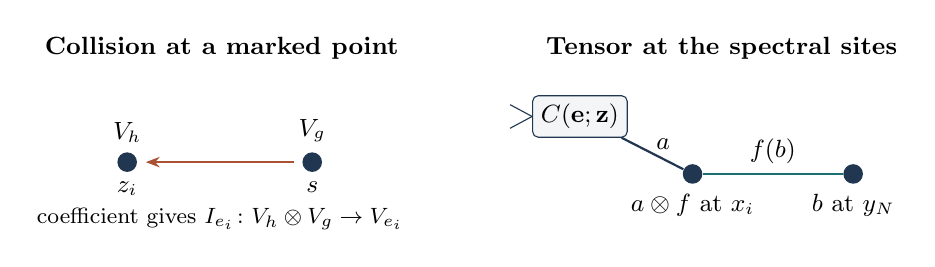
\begin{tikzpicture}[font=\small,x=1cm,y=1cm,
 dot/.style={circle,fill=ink,inner sep=2.5pt},
 gate/.style={draw=ink,rounded corners=2pt,fill=ink!5,inner sep=3pt},
 wire/.style={line width=.9pt,draw=sea}]
 \node[font=\small\bfseries] at (-3.25,1.45) {Collision at a marked point};
 \node[dot,label=below:{$z_i$},label=above:{$V_h$}] (old) at (-4.45,0) {};
 \node[dot,label=below:{$s$},label=above:{$V_g$}] (new) at (-2.10,0) {};
 \draw[-{Stealth[length=5pt]},draw=rust,line width=.8pt]
       ([xshift=-3pt]new.west) -- ([xshift=3pt]old.east);
 \node[font=\footnotesize] at (-3.27,-.72)
       {coefficient gives \(I_{e_i}\colon V_h\otimes V_g\to V_{e_i}\)};

 \node[font=\small\bfseries] at (3.1,1.45) {Tensor at the spectral sites};
 \node[dot,label=below:{$a\otimes f$ at $x_i$}] (xi) at (2.73,-.15) {};
 \node[dot,label=below:{$b$ at $y_N$}] (y) at (4.77,-.15) {};
 \node[gate] (c) at (1.3,.58) {\(C(\mathbf e;\mathbf z)\)};
 \draw[draw=ink,line width=.8pt] (c) -- node[above right,inner sep=1pt] {\(a\)} (xi);
 \draw[wire] (xi) -- node[above] {\(f(b)\)} (y);
 \draw[draw=ink] (c.west) -- ++(-.28,.15);
 \draw[draw=ink] (c.west) -- ++(-.28,-.15);
\end{tikzpicture}
\caption{The collision at \(s=z_i\) supplies a fusion map for each
admissible \(h\). Their span contains \(b\mapsto f(b)a\).
Inserting this map gives the original tensor with input \(a\) and a
wire joining the two spectral sites. The other legs keep their
placements.}\label{fig:sphere-wire}
\end{figure}

The extended scale bounds \(d(x_i,y_N)\le D\). Hence
\eqref{eq:sphere-testwidth} yields \(d(x_i,y_N)\le2\lambda_i u_i+O(v)\).
All constants here are uniform as stated.

The extension can be realized in a complete CAT(0) spectral space.
The closed convex hull of the old sites is canonically isometric to
their original hull by Lemma~\ref{lem:geodesic}.
Projection onto it weakly decreases distances to the old sites.
Consequently
\begin{equation}\label{eq:sphere-Q}
 E\le\sum_i\frac{d(x_i,y_N)^2}{4\lambda_i}
     \le Q_N+O\!\left(\sqrt{\frac{\log(2N)}{N}}\right).
\end{equation}
This is a lower bound on the penalty paid by every optimizer. To turn
it into a lower bound on the optimized price, reuse the same energies
in the objective defining \(B_{N+1}\). Their price is unchanged, while
their penalty in \((N+1)B_{N+1}\) is \(N^2Q_N/(N+1)\), compared with
\(NQ_N\) in \(NB_N\). Thus
\[
 (N+1)B_{N+1}-NB_N\ge\frac{N}{N+1}Q_N.
\]
Sum this inequality and~\eqref{eq:sphere-Q} up to scale \(N\).
The errors sum to \(O(\sqrt{N\log(2N)})\) and \(E\) is uniformly
bounded. Together with \(B_N\le E\) this proves~\eqref{eq:sphere-estimate}.
Equation~\eqref{eq:sphere-squares} now gives the width estimates
in~\eqref{eq:sphere-profile}. The widths and their targets are bounded,
so \(Q_N=E+O(\sqrt{\rho_N})\). Adding \(B_N\) gives the asserted price.
\end{proof}

\subsection{Prescribed widths and uniform comparison}

\begin{corollary}[Prescribed widths]\label{cor:sphere-caps}
Under the hypotheses of Theorem~\ref{thm:sphere}, fix positive width
caps \(a_i\). Then
\begin{equation}\label{eq:sphere-caps}
 \lim_{N\to\infty}
 \frac{1}{N}\max_{\mathbf h:\,w_N(h_i)\le a_i}
            H_{\mathbf x}(C(\mathbf h;\mathbf z))
 = \inf_{o\in X}\sum_i a_i d(o,x_i).
\end{equation}
Convergence is uniform over all placements of bounded scale.
\end{corollary}

\begin{proof}
Transport gives the upper bound. Fix \(\tau>0\) and minimize
\(\sum_i a_i\sqrt{d(o,x_i)^2+\tau^2}\) on the closed convex hull of
the sites. For \(r\) between zero and the hull diameter the function \(r\mapsto\sqrt{r^2+\tau^2}-\epsilon r^2\) is
convex and increasing for sufficiently small \(\epsilon>0\). The CAT(0)
midpoint inequality then makes every minimizing sequence Cauchy, giving
a minimizer by completeness.
Metric projection shows that this is also a minimizer on \(X\).
Write \(r_i=d(o,x_i)\) at this minimizer and set
\(2\lambda_i=\sqrt{r_i^2+\tau^2}/a_i\). The tangent upper bound for the
concave function \(s\mapsto\sqrt{s+\tau^2}\) shows that \(o\) minimizes
\(\sum_i d(o,x_i)^2/(4\lambda_i)\) as well. Indeed the tangent
majorant for the smoothed objective agrees with it at \(o\) and differs
from this quadratic objective by a constant.

At scale bounded by \(D_0\), we have \(r_i\le D_0\). For fixed \(\tau\)
these penalties stay in a compact positive interval. The limiting
widths in~\eqref{eq:sphere-profile} are
\(a_i r_i/\sqrt{r_i^2+\tau^2}\), bounded strictly below \(a_i\) uniformly.
Thus every maximizing tuple at large \(N\) meets the caps. Its normalized
price is
\[
 2E+o(1)
 =\sum_i a_i\frac{r_i^2}{\sqrt{r_i^2+\tau^2}}+o(1)
 \ \ge\ \inf_{z\in X}\sum_i a_i d(z,x_i)-\tau\sum_i a_i+o(1).
\]
Let \(\tau\downarrow0\) after taking \(N\to\infty\).
\end{proof}

A maximizing energy tuple in Corollary~\ref{cor:sphere-caps} can depend
on the placement. The local construction of Section~\ref{subsec:plant-private}
compares a single tensor against all spectral prices simultaneously.
Taking a direct sum over the admissible energies gives that tensor at
a logarithmic cost in each leg dimension.

\begin{corollary}[A common comparison tensor]\label{cor:universal}
Suppose \(\omega_F<9/4\). Fix the \(k\) marked positions and positive
caps \(a_1,\ldots,a_k\). Let \(A_N\) be the direct sum of all nonzero
\(C(\mathbf h;\mathbf z)\) with \(w_N(h_i)\le a_i\) at every leg.
Then
\[
 \frac{H_{\mathbf x}(A_N)}{N}=\inf_{o\in X}\sum_i a_i d(o,x_i)+o(1)
\]
uniformly over placements of bounded scale in complete CAT(0)
spectral spaces over \(F\). The \(i\)th leg of \(A_N\) has log dimension
at most \(Na_i+O_{k,\mathbf a}(\log(2N))\).
\end{corollary}

\begin{proof}
Each leg admits \(O_{\mathbf a}(N^2)\) half-integer energies, so
there are \(O_{k,\mathbf a}(N^{2k})\) summands. Each summand is a
restriction of \(A_N\), and the direct-sum inequality bounds the price
of \(A_N\) by the largest summand price plus
\(O_{k,\mathbf a}(D\log(2N))\). Corollary~\ref{cor:sphere-caps} now
gives the stated limit. Each \(i\)th summand leg has dimension at most
\(e^{Na_i}\) by Lemma~\ref{lem:dimension}, so summing those dimensions
gives the claimed bound.
\end{proof}

\section{Incidence expansion}\label{sec:incidence}

Let $S$ be a finite set of distinct points in an affine plane, and let a
\emph{secant} be a line containing at least two of the points. Write
$\mathcal L$ for the secants and $t_i$ for the number through point $i$.
For centered real labels $v_i$, meaning $\sum_i v_i=0$, we have
\[
 \sum_{L\in\mathcal L}\left|\sum_{i\in S\cap L}v_i\right|^2
       =\sum_{i\in S}(t_i-1)|v_i|^2 .
\]
On expanding the squares, each diagonal term occurs $t_i$ times and
each ordered pair of distinct points occurs once. Centering gives the
identity. We need a version for points placed in a spectral metric space,
where one can measure how far an entire secant pulls a common center
in a given direction. This version will bound the mean squared length
of an incidence edge in the graphs used for permutation routing
(Section~\ref{sec:sort-action}).

\subsection{An inequality for secant lines}

Take $S\subset F^2$ with $|S|\ge2$. For each $i\in S$ choose a site
$x_i$ in a complete $\mathrm{CAT}(0)$ spectral space $X$ over $F$
and a mass $a_i>0$. Let $o$ be the minimizer of
$\sum_i a_i d(o,x_i)^2$ and set $r_i=d(o,x_i)$. Two points of $S$
may be placed at the same site.

Suppose the legs for a subset $C\subset S$ have widths $a_i r_i$.
Sending them from a common site $m$ to their destinations costs
$\sum_{i\in C}a_i r_i d(m,x_i)$. By first variation at $m=o$, the
supremum of the initial savings per unit distance, allowing the common
site to stay at $o$, is
\[
 K_C=\sup_{y\ne o}
       \left(\sum_{i\in C}a_i r_i\cos\angle_o(x_i,y)\right)_+ .
\]
Here $y\in X$, $\angle_o$ is the Alexandrov angle and the summand is
zero if $r_i=0$. For a one-point space set $K_C=0$.
Write $K_L=K_{S\cap L}$. On a real line this is the absolute value of
the secant sum above, with $v_i=a_i(x_i-o)$.

\begin{theorem}[Incidence inequality]\label{thm:incidence}
If $F$ is algebraically closed and $\omega_F<9/4$, then for every
such finite configuration of affine points, weighted sites and secants,
\begin{equation}\label{eq:inc-secants}
       \sum_{L\in\mathcal L}K_L^2
          \le \sum_{i\in S}(t_i-1)a_i^2r_i^2 .
\end{equation}
\end{theorem}

\begin{proof}
Write $i=(u_i,v_i)$ and project the points to the sphere positions
$z_i(s)=u_i s+v_i$. As $s$ varies, a pair collides exactly once on
$\mathbb P^1(F)$, with the projection $i\mapsto u_i$ used at infinity.
Let $D$ consist of the finite collision parameters together with
$\infty$. For each $\alpha\in D$ let $\mathcal P_\alpha$ be the
partition into fibers of its projection. The nonsingleton fibers are
precisely the intersections with secants, each occurring at the
parameter for its direction. Thus $i$ is a singleton at exactly
$|D|-t_i$ parameters, and $K_{\{i\}}=a_i r_i$. Adding these singleton
contributions to both sides of~\eqref{eq:inc-secants} gives the
equivalent estimate
\begin{equation}\label{eq:inc-fibers}
   \sum_{\alpha\in D}\sum_{C\in\mathcal P_\alpha} K_C^2
             \le (|D|-1)\sum_i a_i^2 r_i^2 .
\end{equation}

\emph{Choosing the external widths.}
Fix $s_0\notin D$. The positions $z_i(s_0)$ are distinct, so
Theorem~\ref{thm:sphere} with $\lambda_i=1/(2a_i)$ gives energies
$h_i=h_i(N)$ with
\begin{equation}\label{eq:inc-saturation}
 w_N(h_i)\longrightarrow a_i r_i,\qquad
 \frac{1}{N}H_{\mathbf x}\bigl(C(\mathbf h;\mathbf z(s_0))\bigr)
              \longrightarrow P:=\sum_i a_i r_i^2 .
\end{equation}
Here $w_N(h)=c\sqrt h/N$, $c=\pi/\sqrt3$. The cost of supplying the
external legs from $o$, in these limiting widths, is exactly $P$.
If $P=0$ all $K_C$ vanish. Otherwise take $N$ large enough that the
chosen tensor is nonzero. Its total energy $H_0=\sum_i h_i$ is
$O(N^2)$ and is an integer, since every generator in any nonzero
coefficient is paired.

\emph{A joint bound on the collision energies.}
Write $T(s)=C(\mathbf h;\mathbf z(s))$. In the chart at a finite
$\alpha$ use $s-\alpha$ as coordinate. At infinity use $u=1/s$ and
the positions $u_i+u v_i$. Homogeneity in the positions gives the
tensor $u^{-H_0}T(1/u)$ in this chart. In either chart the points of
each fiber $C$ have a common center and distinct linear offsets.
Proposition~\ref{prop:fusion} expands the coefficient of order $l$
as a sum over intermediate energies $e_C\ge0$ satisfying
$\sum_C e_C=H_0+l$.

Choose temporarily a linear functional $\ell$ with
$f(s)=\ell(T(s))$ nonzero. Let $l_\alpha$ be the order of its first
nonzero coefficient in the corresponding tensor chart. In particular,
$l_\infty=\operatorname{ord}_\infty f-H_0$. The ordinary orders of
$f$ on $\mathbb P^1$ sum to zero. Since there are no poles off $D$,
the energy totals at these orders satisfy
\begin{equation}\label{eq:inc-orders}
  \sum_{\alpha\in D}(H_0+l_\alpha)\le (|D|-1) H_0 .
\end{equation}
Each summand is nonnegative. Using the \emph{same} functional for
all directions is what gives one bound on their total intermediate
energy.

We now require the selected coefficients to retain the price
in~\eqref{eq:inc-saturation}. In every chart collect the fusion terms
with total intermediate energy at most $(|D|-1)H_0$. There are only
polynomially many in $N$. Each term is specified by one nonnegative
half-integer per fiber, and the number of fibers and directions is
fixed. Let $W$ be the span of all collected terms whose price is
less than $H_{\mathbf x}(T(s_0))-\sqrt N$. The ordinary-sum inequality
bounds the price of every nonzero tensor in $W$ by this threshold
plus $O(\log N)$. For large $N$, $T(s_0)\notin W$. Take $\ell$
vanishing on $W$ and nonzero on $T(s_0)$. At each $\alpha$ the
coefficient at its first nonzero order $l_\alpha$ has a fusion term
surviving $\ell$. By~\eqref{eq:inc-orders} such a term was collected,
so its price is at least $H_{\mathbf x}(T(s_0))-\sqrt N$. Select one
surviving term per direction.

Pass to a common subsequence along which the selected widths
$w_N(e_C)$ converge to limits $b_{\alpha,C}$. There are finitely
many widths, all bounded by~\eqref{eq:inc-orders}. Multiplication
of that inequality by $c^2/N^2$ gives
\[
 \sum_{\alpha\in D}\sum_{C\in\mathcal P_\alpha}b_{\alpha,C}^2
                  \le (|D|-1)\sum_i a_i^2 r_i^2 .
\]

\emph{The width needed by one fiber.}
Fix $\alpha$, a fiber $C$, and $y\ne o$. Supply the selected term
by preparing the fused tensor at $o$. Carry the intermediate leg
for $C$ a distance $t$ along $[o,y]$ to a site $m$, apply its fusion
map there and send the external legs from $m$ to their sites. Split
all other legs at $o$. By the transport bound~\eqref{eq:prices-transport}
and $\log\dim V_h\le c\sqrt h$, the price of the selected term is at
most the cost of this supply. After division by $N$, the $\sqrt N$
price loss vanishes. Passing to the limit using~\eqref{eq:inc-saturation} gives
\[
 P\le\sum_{i\notin C}a_i r_i^2+b_{\alpha,C}t+
                       \sum_{i\in C}a_i r_i d(m,x_i).
\]
At $t=0$ equality holds. The derivative from the right is therefore
nonnegative. First variation in a $\mathrm{CAT}(0)$ space gives
$b_{\alpha,C}\ge\sum_{i\in C}a_i r_i\cos\angle_o(x_i,y)$
\cite[Chapter~II.3]{BridsonHaefliger}. Taking the supremum of the
positive part yields $b_{\alpha,C}\ge K_C$, proving~\eqref{eq:inc-fibers}.
\end{proof}

\subsection{The sharp local link inequality}

Suppose $F$ contains $\mathbb F_q$. Take the $q^2$ points of the affine
plane $\mathbb F_q^2$ and retain the lines in $s$ parallel classes,
$1\le s\le q+1$. A point belongs to $s$ retained lines and each line
contains $q$ points. Place the vertices of the resulting bipartite
incidence graph in $X$. Let $e$ be the mean squared distance across a
uniform edge. Give each side half the total mass, uniformly distributed
over its vertices, and let $V$ be the minimum mean squared distance
of this distribution to a common center.

\begin{corollary}[Affine incidence links]\label{cor:inc-link}
Under the hypotheses of Theorem~\ref{thm:incidence},
\[
                   e\ge 2(1-s^{-1/2}) V .
\]
The coefficient is optimal in every target containing a nontrivial
geodesic segment. Omitting one parallel class gives $s=q$ and a
$q$-regular graph on $2q^2$ vertices.
\end{corollary}

\begin{proof}
Take $o$ to be the barycenter of the point sites alone. Write $r_i,r_L$
for the distances from $o$ of a point site $x_i$ and a line site
$y_L$. The mean squared distances on the two sides are
\[
             A=q^{-2}\sum_i r_i^2,\qquad
             B=(sq)^{-1}\sum_{L\ \mathrm{retained}} r_L^2 .
\]
For each incidence, triangle comparison bounds its squared distance
from below by $r_i^2+r_L^2-2r_i r_L\cos\angle_o(x_i,y_L)$.
A zero radius gives a zero cross term. By~\eqref{eq:inc-secants}
with all masses one, $\sum_L K_L^2\le q\sum_i r_i^2$ even for the
full set of lines. Thus the mean cross term over the $s q^2$
retained incidences is at most
\[
 \frac{2}{s q^2}\sum_{L\ \mathrm{retained}}r_L K_L
        \le\frac{2}{s q^2}
           \sqrt{q\sum_i r_i^2\sum_{L\ \mathrm{retained}}r_L^2}
        = 2\sqrt{AB/s}.
\]
Consequently
\[
      e\ge A+B-2\sqrt{AB/s}\ge (1-s^{-1/2})(A+B).
\]
Evaluation at $o$ gives $V\le(A+B)/2$, which proves the corollary.

To attain it, choose one retained parallel class and assign its $q$
lines real labels of mean zero and positive variance. Give each point
the label of its line. Give each line site of that class $\sqrt s$
times its label and every other line site zero. Both sides now have
mean zero and the same mean square $A$. A fraction $1/s$ of the edges
belongs to the chosen class, so the mean product of the two endpoint
labels is $A/\sqrt s$. Hence $V=A$ and
$e=2(1-s^{-1/2})A$. Translate and rescale the labels into any
nontrivial segment of $X$. Nearest-point projection onto the segment
ensures that the ambient minimum has the same value.
\end{proof}

The bound in terms of $A+B$ keeps the point barycenter fixed.
Section~\ref{sec:sort-action} uses that form for affine links, and
uses the secant inequality directly for projective links.


\par\needspace{13\baselineskip}
\part{Sorting and table lookup}\label{part:sorting}
\section{Stable sorting under a strict square saving}\label{sec:sorting}

A tensor network may have to move a table to the place where it will be
used, or bring together all the queries addressed to one table. Moving a table involves long records, while gathering its queries
requires sorting many short ones. We show
that a strict improvement on the exponent $9/4$ would make both operations
cheap enough for the final assembly in Sections~\ref{sec:assembly}
and~\ref{sec:shaving}.

Fix the finite field $k$ from Section~\ref{sec:obstruction} and let $n=2^h$.
The tagged permutation tensor from Section~\ref{sec:list} allows the
destination of every record to be part of the input. Write $j_i$ for
the $h$-bit destination of the $w$-bit source record $x_i$, and $y_j$
for the proposed record at position $j$. Then $\mathrm{Tag}(h,w)$ is the
indicator of the event that the $j_i$ are distinct and $y_{j_i}=x_i$
for every $i$. Similarly, the stable-sort tensor is the indicator that a
proposed output sorts the input records by a designated key and preserves
the input order within each key. Both indicators include the payload bits
in the equality tests.

\begin{theorem}[Conditional stable sorting]\label{thm:sort}
Suppose $\omega_k<9/4$, and let $n=2^h$.
\begin{enumerate}
\item For some $1<p<2$, $\mathrm{Tag}(h,h)$ has an exact trivalent
network over $k$ of size $O(nh^p)$. The same bound holds for stable
sorting of records of at most $ch$ bits, for every fixed $c$.
\item For every $\zeta>0$ there is $a>1$ such that, for every $w\ge h^a$,
both $\mathrm{Tag}(h,w)$ and stable sorting of $w$-bit records have
exact trivalent networks over $k$ of size $O_\zeta(nw h^\zeta)$.
\end{enumerate}
\end{theorem}

\subsection{Evaluating a table by sorting its queries}

At a station of arity $t$, the incident bits give the address of an
entry in a table of length $2^t$. When many copies of the station are
evaluated together, only the multiplicity of each address matters to
the product of the selected entries. Sorting the queries recovers
these multiplicities and spreads the cost of the table over the batch.

\begin{lemma}[Batched table evaluation]\label{lem:batch-table}
Assume the ordinary-width stable-sort bound of Theorem~\ref{thm:sort}
over $k$, with exponent $p>1$. Let a network of binary wires and
$K$-valued tables represent a tensor $T$, where $K/k$ is any field
extension. If $t_v\le u$ is the arity of station $v$ and
$s=\sum_v(1+t_v)$, then $T^{\otimes 2^u}$ has an exact trivalent
$K$-network of size
\[
                  O\bigl(2^u s(1+u)^{p-1}\bigr).
\]
The constant is independent of $K$ and of the entries in the tables.
\end{lemma}

\begin{proof}
First consider one table $f\colon\{0,1\}^t\to K$, with $t\ge1$, and
expose the $2^t$ query addresses $x_1,\ldots,x_{2^t}$ as tensor legs.
If $c_z$ is the number of occurrences of address $z$, the required
product is $\prod_z f(z)^{c_z}$, with an empty product at an unused
address. Create one dictionary row for each $z$ and guess its count in
$t+1$ bits. On count bit $j$, for $0\le j\le t$, place a unary factor
with entries
\[
                    (1,\ f(z)^{2^j}).
\]
The position of this factor already determines $z$. Thus its two entries
are fixed coefficients of the network.

Give each query its own row, with zeros in the count field. Sort the
$2^{t+1}$ rows by address and then by row type, so that the dictionary
row follows all queries to that address. A counter, initially zero,
increments on every query. On a dictionary row it must agree with the
carried count and then resets to zero. This checks the count even at
addresses with no queries. For fixed exposed addresses there is exactly
one valid choice of counts, sorted rows and counter states. The
contraction therefore equals $\prod_i f(x_i)$ in every characteristic,
also when a table entry vanishes.

The counter uses $O(2^t(1+t))$ gates by ripple-carry addition.
Sorting the $O(t+1)$-bit rows costs $O(2^t(1+t)^p)$. The sorting
network realizes a zero--one tensor over $k$ and hence realizes the
same tensor over $K$ by scalar extension.

Group the $2^u$ copies of each station of arity $t$ into $2^{u-t}$
batches of $2^t$. A station of arity zero supplies a scalar directly.
Connect the exposed wires according to the original network in each
copy. The result contracts to $T^{\otimes 2^u}$ and its size is
bounded by a constant times
\[
  2^u\sum_v(1+t_v)^p
       \ \le\ 2^u(1+u)^{p-1}\sum_v(1+t_v).
\]
\end{proof}


\subsection{The two scales of the sorting proof}\label{sec:sort-road}

Assume $\omega_k<9/4$ throughout Part~II. We first route wide records.
A hop that permutes records within a smaller address set can be handled
recursively. The objective is to shorten the address by an arbitrarily
large constant factor while keeping the total width transported in each summand within a
constant multiple of the input width, independently of that factor. Repeating such
a reduction gives the wide-record estimate in Theorem~\ref{thm:sort}.
Once that estimate is available, two levels of radix sorting give the
ordinary-width estimate. A short key selects a digit within a block,
and whole packs of records with the same digit then travel together.

Section~\ref{sec:sort-action} uses the incidence inequalities of Part~I
to compare the price of a target permutation with the prices of hops on
smaller sets of addresses. The comparison first holds for an action on
a CAT(0) space. Local price data sufficient to realize such an action
give the same bound. If the data fail a local consistency test, spectral
comparison instead supplies a tensor identity that reduces the cost.
Section~\ref{sec:sort-route} combines these two conclusions to route
payloads and to bound the number of recursive calls in a fixed network.

Throughout Parts~II--IV we use base-two logarithms for ordinary prices.
In these units the distance $d$ is the price of carrying one bit.
On a fixed finite list of sites, price data with bounded scale,
including scale zero, form a compact set by \eqref{eq:prices-range}
and Section~\ref{sec:prices-background}. A bound on diameter suffices
here. Equality along a spanning tree of binary wires realizes the
full diagonal and bounds its price.

Distances between sites obtained by finitely many geodesic interpolations
at fixed fractions depend continuously on the original prices. The
enlarged configurations still have bounded scale. Along any convergent
subnet the interpolation equalities pass to the limit, where
Lemma~\ref{lem:geodesic} determines the distances from the original data.


\section{From incidence to permutation actions}\label{sec:sort-action}

A permutation can be factored into hops that change only a short
part of the address. Adding their prices gives a bound proportional
to the number of factors. Sorting with wide records requires a
bound independent of that number. We first obtain such a bound on
displacement in a metric space. We then show that finite tests on
the addresses suffice to bound the mean price of the payload wires.

\subsection{Two incidence inequalities}

Fix a power $q\ge100$ of the characteristic of $k$. In a placement
of a bipartite incidence graph, a vertex on either side is assigned
a site. The incidence energy $e$ is the mean squared distance between
sites at the ends of a uniform incidence.

\begin{lemma}\label{lem:sort-inc}
Suppose $\omega_k<9/4$. In any complete $\operatorname{CAT}(0)$
spectral space over $k$, consider a placement of either of the
following graphs.
\begin{enumerate}
\item The points and lines of the projective space $\mathrm{PG}(\ell-1,q)$,
where $\ell\ge3$.
\item The points of $\mathbb F_Q^2$ and the affine lines in the $q+1$
directions defined over $\mathbb F_q$, where $Q=q^R$.
\end{enumerate}
Let $o$ be the barycenter of the point sites. Let $A$ and $B$ be
the mean squared distances to $o$ on the point and line sides,
respectively, with uniform weights on each side. Then
\[
                 e\ge (1-q^{-1/2})(A+B).
\]
\end{lemma}

\begin{proof}
The field $\bar k$ contains every $\mathbb F_Q$ in the statement
and satisfies $\omega_{\bar k}\le\omega_k$. To apply
Theorem~\ref{thm:incidence} there, recall that scalar extension
preserves the possible joint spectral evaluations on any finite
placement of $k$-tensors (Section~\ref{sec:prices-background}).
In particular, each finite subset of our metric space has an isometric
realization in a complete spectral space over $\bar k$. Take a pointed
ultralimit of these realizations over the finite subsets containing a
fixed basepoint, using an ultrafilter containing every tail under inclusion.
Each original site is eventually present with all its prescribed
distances. Completeness and uniqueness of geodesics make the resulting
isometric image closed and convex. For a bounded finite distribution
in the ultralimit, the barycentric variance inequality identifies its
barycenter with the limit of the coordinate barycenters. For a
distribution in the image, nearest-point projection places its
barycenter in the image as well. It therefore suffices to prove the
inequalities on placements over $\bar k$.

For the affine plane, apply the unit-mass estimate in the proof of
Corollary~\ref{cor:inc-link} to the configuration $\mathbb F_Q^2\subset\bar k^2$, retaining $q+1$
directions. It bounds the cross term in squared-distance comparison
by $2\sqrt{AB/(q+1)}$, giving the assertion.

For the projective space, map $\bar k^\ell$ linearly into $\bar k^3$,
preserving the ranks of sets of up to three projective
representatives. Such maps form a nonempty open set. Indeed, preserving
each rank is a nonempty open condition and there are only finitely many
conditions. In the resulting projective plane choose an affine chart
containing all the images. Preservation of pairs and triples makes the
images distinct and preserves exactly which triples are collinear.
The secants of the affine configuration thus represent the lines of
the original projective space.

There are $j$ lines through each point and $s=q+1$ points on each line.
Write $r_i=d(o,x_i)$ for point sites and $r_L=d(o,y_L)$ for line sites.
Set
\[
 K_L=\sup_{z\ne o}\Bigl(\sum_{i\in L}
       r_i\cos\angle_o(x_i,z)\Bigr)_+ ,
\]
with zero summands at $r_i=0$. The singleton space satisfies the
claim directly. In every other case Theorem~\ref{thm:incidence}
gives $\sum_L K_L^2\le (j-1)\sum_i r_i^2$. If $M$ is the number of
incidences, triangle comparison and Cauchy--Schwarz bound the mean
cross term by
\[
 \frac{2}{M}\sum_L r_L K_L
 \le 2\sqrt{\frac{j-1}{js}AB}
 \le q^{-1/2}(A+B).
\]
Here $M$ is both $j$ times the number of points and $s$ times the
number of lines. Subtracting the cross term from $A+B$ proves the claim.
\end{proof}

\subsection{Permutations on short address sets}

Choose an integer $\ell\ge3$ and reserve $m$ auxiliary coordinates,
where $m$ will depend only on $q$. For $n=2^h$ put
\[
 r=\left\lfloor \frac{\log_q n}{\ell+m}\right\rfloor,\qquad
 U=\mathbb F_q^r,\quad N=q^r,\quad
 c=\left\lceil n/N^{\ell+m}\right\rceil,\qquad
 \mathcal I=U^\ell\times[c]\times U^m .
\]
Here $[c]=\{1,\ldots,c\}$. Identify the original $n$ addresses with
the first $n$ labels in a fixed ordering of $\mathcal I$ and extend
the input permutation $\pi$ by fixed points. The padded address set
satisfies $n\le|\mathcal I|<2n$.

A \emph{permutation function} takes a height $h$ and a valid input
permutation as parameters and outputs a permutation of $\mathcal I$.
We require a single deterministic program using $nh^{O(1)}$ operations
on words of $O(h)$ bits, with the usual word operations of polynomial
bit complexity. These functions form a countable group $G$ under
pointwise composition. An explicitly listed permutation has a
linear-time inverse, and $\pi$ itself is an element of $G$.

Identify $U^\ell$ with $\mathbb F_q^\ell\otimes U$. For a fixed
subspace $V\le\mathbb F_q^\ell$ of dimension at most two, let $K_V$
be the subgroup preserving every fiber of the projection
$\mathcal I\to(\mathbb F_q^\ell/V)\otimes U$. All auxiliary labels
belong to the fiber. Its size is $cN^{m+\dim V}$, so every hop in
$K_V$ permutes sets of size at most $2^{th+O(1)}$, where
\begin{equation}\label{eq:sort-hop-height}
                         t=\frac{m+2}{m+\ell}.
\end{equation}
The additive constant follows from $c\le q^{m+\ell}$. Increasing
$\ell$ shortens the address within a fiber.

The subgroups $K_V$ generate $G$. We give the coordinate factorization
of a rearrangeable network \cite{benes} in algorithmic form because
the routing protocol will use its factors. Treat $[c]\times U^m$ as
one coordinate. To eliminate a coordinate of size $a$, form a bipartite
multigraph on the remaining input and output names, with one edge per
requested transfer. Each vertex has degree $a$. Give the edges $a$
colors, using each color once at each vertex. In the first stage,
permute the chosen coordinate to its edge color. In the last stage,
permute that color to the destination coordinate. Between these stages
the remaining coordinates are permuted separately for each color.
Iterating gives a bounded number of stages for fixed $\ell,m$.
Each ordinary coordinate stage is in its coordinate line subgroup,
and each auxiliary stage is in $K_0$.

For completeness, the coloring takes deterministic time linear in
the edge count up to logarithmic factors (see also \cite{color}).
An even-regular bipartite multigraph splits into two regular halves
by alternating colors around Euler tours. At an odd degree $a$ we first
remove one perfect matching. To find it, let $v$ be the number of
vertices on each side and take the least $H$ with $2^H>av$. Multiply
each edge multiplicity by $\lfloor 2^H/a\rfloor$ and complete the
graph to degree $2^H$ with copies of an arbitrary dummy matching. The
total dummy multiplicity is less than $av<2^H$. Split into regular
halves repeatedly, keeping the half with fewer dummy copies and
breaking ties deterministically. Each split divides even multiplicities
equally and alternates the remaining odd copies around Euler tours,
distinguishing dummy from original edges. After $H$ splits the retained
degree-one graph has no dummy copy. Only the original edges and the
dummy matching need be stored, with multiplicities fitting in a word.
After the matching is removed the residual even degree splits in half,
so the full coloring recursion has logarithmically many levels.

\subsection{Uniform displacement}

A bound obtained by adding displacements along the coordinate
factorization would depend on $\ell$. The fixed point in the next
lemma bounds the displacement of every product of hops by a single
absolute constant.

\begin{lemma}\label{lem:sort-geometry}
Suppose $G$ acts isometrically on a complete $\operatorname{CAT}(0)$
space $Y$ in which the inequalities of Lemma~\ref{lem:sort-inc}
hold for all placements. There is an absolute constant $C_0$ such
that, if $d(x,gx)\le1$ for all $g\in\bigcup_V K_V$, then $G$ fixes
a point within $C_0/2$ of $x$. In particular $d(x,\pi x)\le C_0$.
\end{lemma}

\begin{proof}
Use a triangle for each flag $0\subset L\subset P$, where $L$ is
a vector line and $P$ a vector plane in $\mathbb F_q^\ell$. We use
the link-energy argument of Garland and its metric fixed-point
version \cite{garland,izekinayatani}. Choose the flag uniformly and,
within it, a vertex or edge uniformly. A placement assigns each $V$
a point $y_V$ fixed by $K_V$. For each $V$ we seek another such point
$z_V$ so that, in a uniform flag through $V$,
\begin{equation}\label{eq:sort-flag-link}
 \mathbb E\,d(z_V,y_W)^2\le \tfrac34\,
                           \mathbb E\,d(y_{W_1},y_{W_2})^2 .
\end{equation}
The vertices $W_1,W_2$ lie opposite $V$, and $W$ is uniform among them.
At $V=0$, the opposite edges are the incidences of projective points
$L$ and projective lines $P$. The barycenter of the $y_L$ is fixed
by $K_0$. Lemma~\ref{lem:sort-inc} bounds its mean squared distance
to a neighbor by $1/[2(1-q^{-1/2})]$ times the opposite-edge energy.
At $V=L$, the barycenter of the $y_P$ with $P\supset L$ is fixed by
$K_L$. Its variance inequality with test point $y_0$ gives the
coefficient $1/2$.

\smallskip\noindent
\emph{The plane vertex.}
When $V=P$, the opposite edge joins $0$ to a line $L\subset P$.
Here $y_0$ and the $y_L$ need not be fixed by $K_P$. We use translates
of these sites to build an affine incidence graph of the same edge
energy. The point barycenter of this graph will be nearly fixed by
$K_P$.

Choose coordinates $(x_1,x_2)\in U^2$ along $P$ in each fiber
modulo $P$, using a fixed basis and linear complement. Each coordinate
pair names a class of $cN^m$ labels. Consider any other partition of
each fiber into classes with these same names and cardinalities,
computed uniformly at all heights and inputs in the time defining
$G$. It is obtained from the coordinate partition by some $g\in K_P$,
by sorting and matching equal names within fibers. Explicitly, if $p$
is the coordinate name, the transported name is $p\circ g^{-1}$.
Assign the new partition the site $g y_0$. Any other such $g$ differs on the right by an element
of $K_0$, so this site is well defined. Projecting the names modulo
$L\otimes U$ gives a coarser partition to which we assign $g y_L$.
The stabilizer of the reference projected partition is $K_L$.
Both assignments commute with
the action of $K_P$. Thus a partition and its projection have site
distance exactly $d(y_0,y_L)$.

Let $Q=q^R$, where $R\le m$ will be chosen below. Use $R$ auxiliary
$U$-coordinates as the values of an $\mathbb F_q$-linear map
$u:\mathbb F_Q\to U$ on a fixed basis of $\mathbb F_Q$. For a uniform
label in a fiber, $u$ is uniform independently of $(x_1,x_2)$. For
each $(a,b)\in\mathbb F_Q^2$ form the partition with name
$(x_1+u(a),x_2+u(b))$. The name is uniform on $U^2$. Along an affine
line of direction $L$ defined over $\mathbb F_q$, the name modulo
$L\otimes U$ is constant as a function of $(a,b)$, by linearity of
$u$. We therefore obtain sites for all points and all retained lines.
The incidence energy is $e_P=\mathbb E_{L\subset P}d(y_0,y_L)^2$.
At the point barycenter $b_0$, Lemma~\ref{lem:sort-inc} now gives
$(1-q^{-1/2})(A+B)\le e_P$.

\smallskip\noindent
\emph{A fixed center.}
For $d_*$ independent samples from the point-site distribution, form
a successive geodesic mean by moving a fraction $1/i$ toward sample
$i$ at step $i$. Its final value $M_{d_*}$ satisfies
\begin{equation}\label{eq:sort-mean}
                  \mathbb E\,d(M_{d_*},b_0)^2\le A/d_*.
\end{equation}
Indeed, condition on the previous mean. Squared-distance convexity
and the variance inequality at $b_0$ bound the new expected squared
error by $(1-1/i)^2$ times the old error plus $A/i^2$.

Call a tuple of partitions independent if its joint names are uniform
in every fiber at every height and input. This is a property of a
realized tuple. Choose a large absolute integer $d_*$ and set $m=R=4d_*$.
For $4d_*$ independent uniform samples from $\mathbb F_Q$, the probability
of a linear dependence over $\mathbb F_q$ is at most
$\sum_{j=0}^{R-1}q^{j-R}<1/(q-1)$. With probability at least $1/2$, the
two coordinates of each of $2d_*$ sampled affine points give $4d_*$
linearly independent field elements. Evaluation of $u$ on them is
then jointly uniform even conditional on $(x_1,x_2)$, so the $2d_*$
partitions are independent.

The group $K_P$ is transitive on the efficiently specified independent
tuples of this length, by matching joint names within each fiber.
Consequently the distance between the means of the two halves is the
same for all such tuples. Its unconditional expected square is at most
$4A/d_*$ by \eqref{eq:sort-mean} and the triangle inequality. For
each independent tuple the square is therefore at most $8A/d_*$.
The same conditioning gives an independent $d_*$-tuple of affine
partitions whose mean $M$ satisfies $d(M,b_0)^2\le2A/d_*$.

Fix $g\in K_P$. The tuple giving $M$ and its $g$-translate may be
dependent. Construct a third tuple jointly independent with each of
them separately. In each fiber join the old name at a label to its
translated name by one edge for that label. Both sides of the resulting
bipartite graph have $N^{2d_*}$ vertices, each of degree
$cN^{m+2-2d_*}$. The degree is divisible by $N^{2d_*}$. Color its
edges properly as above and group the colors into $N^{2d_*}$ sets of
equal size. Regard the color set of an edge as its third name in
$U^{2d_*}$. At every vertex, each third name occurs equally often,
which proves the two required independence statements. The coloring
also supplies the third tuple in the time defining $G$.

The mean of this tuple lies within $\sqrt{8A/d_*}$ of both $M$ and
$gM$. Hence
\[
 d(b_0,gb_0)\le 2\bigl(\sqrt{2A/d_*}+\sqrt{8A/d_*}\bigr)
                      \le 0.04\sqrt A
\]
on choosing $d_*$ sufficiently large. The circumcenter $z_P$ of the
$K_P$-orbit of $b_0$ is fixed by $K_P$ and lies within $0.04\sqrt A$
of $b_0$. With half the mass on each side of the affine incidence graph,
the root mean squared distance to $z_P$ is at most
$\sqrt{(A+B)/2}+0.04\sqrt A$. In this average an affine point site is a
translate of $y_0$, and an affine line site of direction $L$ is a
translate of $y_L$. Since $z_P$ is fixed, these distances are precisely
the distances from $z_P$ to $y_0$ and $y_L$. The inequality
$(1/\sqrt2+0.04)^2/(1-q^{-1/2})<3/4$ proves
\eqref{eq:sort-flag-link} at $P$.

\smallskip\noindent
\emph{Iteration on the flags.}
Initialize $y_V$ at the circumcenter of $K_Vx$, within distance one of
$x$. Replace each $y_V$ by its midpoint with $z_V$, which is still fixed
by $K_V$. Write $e$ for the mean squared edge length of a flag. By
convexity of distance between geodesics, the squared distance between
the new endpoints at $V,W$ is at most
$\bigl(d(y_V,z_W)^2+d(z_V,y_W)^2\bigr)/2$.
Averaging \eqref{eq:sort-flag-link} over flags thus gives
$e_{\rm new}\le3e/4$. By the triangle inequality through a random old
neighbor, the root mean squared movement per vertex is at most
$(\sqrt e+\sqrt{3e/4})/2\le\sqrt e$.
Initially $e\le4$. The movements are summable in the finite weighted
metric product, and each edge in its limit has length zero. The flag
graph is connected, so the limiting placement has a single value
$y_*$. This value is fixed by all the $K_V$ and hence by $G$.
Summing the movements gives $d(x,y_*)\le1+2/(1-\sqrt{3/4})$.
We may take $C_0=100$.
\end{proof}

\subsection{Finite tests on permutation orbits}

We now return to the finite set of addresses. In the routing protocol
a proposed price is assigned separately to each payload wire. We will
test these prices in balls of bounded radius. To compare price
realizations on overlapping balls we must also test the other tensors
on their common sites.

Take a finite symmetric set of elements of $\bigcup_V K_V$ containing
the factors of a fixed coordinate factorization of $\pi$ and their
inverses. Call these the \emph{core generators}. For each input they
define an undirected graph on $\mathcal I$, with a \emph{core link}
for the hop from a label to its image under a generator. Its degree
is bounded by the size of the set. Each $i$ has a path to $\pi(i)$
along the factors, of length bounded by a fixed rational $a_{\mathrm p}$
independently of $h$ and the input.

The four test parameters are the core generators, a ball radius,
a maximum number of sites, and a maximum local dimension. Give each
payload wire its own commodity index. Also index every nonzero $k$-tensor
of permitted format on an ordered list of distinct sites in a common
test ball, using fixed coordinate bases. Assign this index on the
whole graph, so two balls containing the same tensor on the same
ordered sites see one price. There are $O(|\mathcal I|)$ indices
because each ball has bounded size and the field is finite.

Assign each commodity a nonnegative price. Cap a payload price at
$a_{\mathrm p}$. For each other format choose a uniform rational cap
sufficient to create the tensor at one site and transport its legs in
binary coordinates along core links in the ball. On a test ball compare
the assigned prices of all its commodities with an ordinary spectral
price on its sites. The error is the largest absolute discrepancy on a
commodity or positive excess above unit cost on a core link with both
endpoints in the ball. Duplicate commodities are compared separately
with the spectral price of the same tensor. The minimum error over ordinary prices, allowing the collapsed price,
is the \emph{discrepancy} of the test. This minimum is attained.
Indeed, the core links connect the ball, so a spanning tree bounds
the scale of any price with bounded error, and prices at bounded scale
form a compact set. On a singleton use the collapsed price. A center
\emph{passes} to tolerance $\rho$ if this minimum is at most $\rho$.

\begin{lemma}[Finite detection]\label{lem:sort-local-tests}
For each $\ell$ there are finite test parameters and $\rho>0$ such
that the following holds for all sufficiently large $h$ and every
valid permutation input. If all but a fraction $\rho$ of the centers
pass to tolerance $\rho$, the assigned payload prices satisfy
\[
        |\mathcal I|^{-1}\sum_{i\in\mathcal I} x_{i,\pi(i)}
                  \le C_0+1 .
\]
Here $C_0$ is the absolute constant of Lemma~\ref{lem:sort-geometry}.
\end{lemma}

\begin{proof}
If the assertion fails, choose a sequence of counterexamples with
$h\to\infty$. Enlarge the finite symmetric sets of core generators
to exhaust the countable union of the $K_V$, and let the radii and format
bounds tend to infinity. Take the tolerance and permitted exceptional
fraction tending to zero, keeping the original factorization of $\pi$
and the payload cap fixed. We use these counterexamples to construct
an action in which each hop has displacement at most one and the
target permutation has displacement at least $C_0+1$.

\smallskip\noindent
\emph{The marked sites.}
At each passing center $i$ take a complete $\operatorname{CAT}(0)$
spectral realization of a price attaining the test. At every other
center use the one-point space. For $g\in G$ mark the site $g^{-1}i$
in the chart at $i$. A fixed word in subgroup elements represents
$g^{-1}$, so eventually these hops are tested and the ball contains
the whole path from $i$ to $g^{-1}i$. Thus the distance from the
center to this mark is uniformly bounded for each fixed $g$.
Use the center itself when the mark is unavailable.

At each index take the metric product over all centers with the
root mean square distance, pointed at the vector of centers.
Take a pointed ultralimit of the products and let $Y$ be the closed
convex hull of the resulting marks. The product and ultralimit are
complete $\operatorname{CAT}(0)$ spaces, as one sees from the
midpoint inequality. Both incidence bounds of Lemma~\ref{lem:sort-inc}
hold in $Y$. A product barycenter is coordinatewise, so the squared
inequalities average over the coordinates. In the ultralimit the
variance inequality identifies the limit of barycenters with the
barycenter of a bounded finite placement. Finally, projection onto a
closed convex subset preserves the barycenter of a distribution in
that subset.

\smallskip\noindent
\emph{Translation of the marks.}
We claim that left multiplication $g\mapsto ug$ extends to an
isometry of $Y$. A point of a dense subset of $Y$ is given by a
finite expression of geodesic interpolations of marks. Fix two such
expressions. At center $i$ the translated expressions have the
same underlying address labels as the original expressions at center
$u^{-1}i$, since $(ug)^{-1}i=g^{-1}u^{-1}i$.

For sufficiently large indices, both balls contain these labels.
Both centers pass outside a fraction tending to zero, since
$i\mapsto u^{-1}i$ preserves uniform measure. For every fixed tensor
on the distinct labels the two realizations then differ by at most
twice the tolerance once the format bounds include that tensor.
Their evaluations use its common commodity index. It follows that
the distances between the two expressions in the two charts differ
by a quantity tending uniformly to zero on such pairs. Indeed, a
violating sequence has a subsequence with a fixed pattern of coincident
labels. The finitely many factor words bound the diameter of the
marked list in both charts, so the tree estimate bounds their price
scales. By compactness take limiting prices on the list. They agree
on every tensor by the format exhaustion. Continuity of distances
between geodesic expressions, from Lemma~\ref{lem:geodesic}, gives
equal limiting distances, a contradiction.

All expression distances are bounded even on exceptional pairs.
In a passing chart the fixed word lengths bound all the marks, and
a failed chart has collapsed to a point. The exceptional pairs
therefore make a vanishing contribution to the squared mean. Reindexing
by $i\mapsto u^{-1}i$ proves the claimed equality of distances in the
limit. The assignment on expressions thus extends to $Y$. Its inverse
comes from $u^{-1}$, and the group law holds first on expressions and
then by continuity on $Y$.

Let $x$ be the identity mark. For each individual $g\in K_V$ its hop
and inverse eventually belong to the tested set, so $d(x,gx)\le1$.
The mark $\pi^{-1}x$ at center $i$ corresponds to the address $\pi(i)$.
In a passing chart its distance from the center agrees up to the
tolerance with the assigned price of the payload wire $i\to\pi(i)$.
In a failed chart the distance is zero while the price is at most
$a_{\mathrm p}$. Thus $d(x,\pi^{-1}x)$ is the ultralimit of the root
mean square payload price. This is at least the limiting lower bound
$C_0+1$ on the arithmetic means of the counterexamples.
Since $d(x,\pi^{-1}x)=d(x,\pi x)$, this contradicts
Lemma~\ref{lem:sort-geometry}.
\end{proof}


\section{Bounded-width permutation routing}\label{sec:sort-route}
\subsection{From a failed price test to a routing identity}

Fix the core generators and the test parameters of
Lemma~\ref{lem:sort-local-tests}. Write $M=|\mathcal I|$, so that
$n\le M<2n$. Sending a bit along the designated path from $i$ to
$\pi(i)$ pays for every hop on that path. We seek an exact sum of
networks in which the average transport cost per payload bit has an
absolute bound, even as the parameter $\ell$ increases.

\begin{proposition}\label{prop:sort-protocol}
Suppose $\omega_k<9/4$ and fix $H\ge1$. For all sufficiently large
$h$, every valid set of tags and every $h\le w\le h^H$, the associated
permutation tensor for $w$-bit payloads is an exact sum over $k$ of
networks with the following properties.
\begin{enumerate}
\item Each label has a bounded number of fixed slots per core generator.
A used slot carries $O(w)$ bits to a neighbor along the generator or its
inverse. Both ends belong to the same prescribed group of at most
$2^{th+O(1)}$ labels. The sum of the carried widths in any summand is
at most $Cnw$, where $C$ is independent of $\ell$ and $t$.
\item At each label a fixed trivalent network of size
$O(w(1+\log w)^{O(1)})$ implements the local maps. Its configuration
consists of a bounded list of menu indices, widths and offsets.
\item A summand is specified by $O(n\log(2w))$ bits. Given these bits
and the tags, a deterministic controller computes the local
configurations and matchings in $nh^{O(1)}$ word operations.
The exponents and slot capacities are independent of $H$. The running
time may have a multiplicative constant depending on $H$.
\end{enumerate}
\end{proposition}

\begin{proof}
We use the local replacement argument of
\cite[Section~\ext{G}{sec:protocol}]{oaG}. A \emph{request} for a
commodity leaves that tensor to be supplied at specified legs.
Its cap $a_i$ bounds the cost of supplying it directly, by preparing
the tensor at one site and sending its legs along designated core
paths. We encode each leg in binary and pad its unused coordinates
by zero. Multilinearity permits us to substitute a tensor identity
for several requests at any stage of a contraction.

\smallskip\noindent
\emph{The identity on a ball.}
Let $x\in\prod_i[0,a_i]$ be a price array with positive discrepancy on
a ball. Request one copy of each commodity with $x_i>0$ on the ball.
Their tensor product $D$ has assigned total price $L=\sum_{i:x_i>0}x_i>0$,
since the zero array passes the test. The available supplies $T_j$
are all the commodities on the ball, at their assigned prices, and
its binary core links, at price one. On a singleton we can prepare
every demand locally. On a larger ball there are prices $l_j$ strictly
above the supply prices and a number $0<L_-<L$ such that every
normalized spectral log price $P$ satisfies
\[
                 P(D)<L_-\max_j\frac{P(T_j)}{l_j}.
\]
Indeed a spanning tree of binary core links supplies the full binary
diagonal, of normalized log price one. Thus the maximum ratio is at
least the reciprocal of the sum of the $l_j$ over the tree. If the
strict inequality with $L$ failed for perturbations decreasing to
the original supply prices, rescale each violating $P$ by dividing
by its maximum ratio. The tree bound keeps the scales bounded.
A limit price then satisfies every supply bound and gives $D$ price
at least $L$. Additivity on products forces equality at each
positive-priced commodity, and the remaining commodities have price
zero. This limit would pass the test on the ball. For a fixed
successful perturbation, compactness permits the decrease from $L$
to $L_-$ with a uniform strict margin.

Choose an integer $b_0$ and form the direct sum
\[
               U=\bigoplus_j T_j^{\otimes\lfloor b_0L_-/l_j\rfloor}.
\]
Rounding costs a bounded amount in log price. For sufficiently large
$b_0$, every normalized spectral price gives $U$ a higher value than
$D^{\otimes b_0}$. Strict spectral comparison in
Section~\ref{sec:prices-background} now gives an exact restriction of
$D^{\otimes b_0r}$ from at most $K(b_0)$ direct copies of
$U^{\otimes r}$ for every $r\ge1$. Expand the direct sums and apply
the restricting maps. The resulting ordinary sum supplies $b=b_0r$
copies of every demand. Each term uses supplies of total price at
most $bL_-$. Its index specifies a direct copy and an ordered word
of $r$ supply choices. With $s$ supply types this takes at most
$\lceil\log_2(K(b_0)s^r)\rceil$ bits. The ratio of this length to
$b$ can be made arbitrarily small by first increasing $b_0$ and then
$r$.

Repeat the identity $J$ times. Use only the \emph{histogram} of the
$J$ term indices as the outer selector. This costs $O(\log(2J))$
bits because the alphabet is fixed. Within the corresponding network
a root sums over ordered words, sends each word along the core tree
and enforces its prescribed histogram. The histogram fixes the
number of copies of every supply. The word assigns these copies to
the individual applications of the restricting maps. Each ordered
word contributes exactly once with its original coefficient over
$k$. Choose the rate of the term indices low enough that the tree
transmission costs at most $Jb(L-L_-)/2$. The replacement thus saves
a positive amount per block of demands, after paying for its own
control bits.

These demands remain positively priced, and the replacement retains
a strict saving, throughout a neighborhood of the original array.
There are finitely many ball types since the field, radius, degrees
and formats are fixed. Compactness of the price arrays of discrepancy
at least $\rho/2$ gives a finite menu of replacements. On this set,
the saving per unit of demand and the selected demand prices both
have uniform positive lower bounds.

\smallskip\noindent
\emph{Bounding the total width.}
Follow one summand in the expansion. Let $wz_i$ be its integer stock
of outstanding requests for commodity $i$, and let $S$ be its
installed core width divided by $Mw$. Give the summand the account
$S+F(z)$, where
\[
       F(z)=\frac1M\max_{0\le x\le a}
                   \sum_i\bigl(z_ix_i-\tfrac12\mu x_i^2\bigr).
\]
There are $O(M)$ coordinates with uniformly bounded caps. Choose
a positive rational $\mu$ such that $\mu\sum_i a_i^2/(2M)\le1$.
The maximizing price $x_i=\min(a_i,z_i/\mu)$ satisfies
$z_i\ge\mu x_i$. Its Lipschitz bound gives, for $z+v\ge0$,
\[
       F(z+v)-F(z)
       \le \frac1M\sum_i x_iv_i+\frac1{2\mu M}\sum_i v_i^2 .
\]
Fix an integer $B>\max_i\mu a_i$. Whenever a stock exceeds $wB$,
supply the excess directly. On the interval $z_i\ge B$ the
marginal price equals $a_i$, so this operation does not increase
the account.

If the mean maximizing price of the $M$ payloads exceeds $C_0+2$,
Lemma~\ref{lem:sort-local-tests} gives more than $\rho M$ balls of
discrepancy greater than $\rho$. A greedy packing selects $\Omega(M)$
disjoint such balls, allowing a fixed slack in the test. Indeed the
discrepancy is $1$-Lipschitz in the array of prices. A sufficiently
fine rational grid can assign a valid menu entry to each cell meeting
the set of discrepancy at least $\rho$, with the entry valid throughout
the cell. These finite tables suffice to select and pack eligible balls.

On each packed ball apply its replacement with
$J=\lfloor\alpha w/b\rfloor$, for a small fixed rational $\alpha>0$.
The bound $z_i\ge\mu x_i$ and the positive lower bound on selected
demand prices ensure sufficient stock. Charge each new core link to
$S$, and enter other supplies as new requests. In the linear bound on
the account, each ball saves a fixed positive amount per retired demand
block, including transmission of the word. For large $w$ the packed
balls therefore save at least $c\alpha$ in the normalized account for
some $c>0$. The finite menu and the disjoint balls give
$\max_i|v_i|=O(\alpha)$, so the quadratic error is $O(\alpha^2)$.
Fix $\alpha$ small enough that each parallel round lowers the account
by a fixed positive amount in every resulting summand. Supply any
excess over the stock cap after the round.

Starting from zero, introduce all $w$ copies of each payload in equal
increments on a fixed fine mesh, rounding to integers with exact total
$w$. Before each increment use parallel rounds until the mean payload
price is at most $C_0+2$. The account is nonnegative. The increments
have total linear cost at most $C_0+2$, and their summed quadratic
cost is at most one for a sufficiently fine mesh and sufficiently
large $w$. Supply excess stock after each increment. Every summand
therefore undergoes only boundedly many rounds, and its final account
is at most $C_0+3$. Supply all the remaining requests directly.
Taking $x=a$ in the definition of $F$ gives
\[
             \frac1M\sum_i a_i z_i\le F(z)+1.
\]
The total width is at most $(C_0+4)Mw\le 2(C_0+4)nw$. This last
coefficient is absolute.

\smallskip\noindent
\emph{Realizing the summands.}
A label lies in at most one packed ball per round. Every direct
supply that uses a given edge originates within bounded distance of
it. Bounded degree, boundedly many commodity types per neighborhood,
and the stock cap thus give boundedly many slots of width $O(w)$
per generator. The generator prescribes the group containing both
ends of the slot.

At the sites of a commodity, keep its requests in common order,
retiring them from the front and appending new requests at the back.
For each replacement the histogram determines the lengths of the
lists. Inside its network, prefix counts of the ordered word assign
supply positions to repeated applications. Comparison sorting on
addresses of $O(1+\log w)$ bits realizes these permutations and
partial matchings with $O(w(1+\log w)^{O(1)})$ trivalent gates at a
site. Complete partial matchings deterministically and set idle
coordinates to zero. Each individual block map has fixed size over
$k$ and admits a constant-size trivalent implementation. Only
boundedly many local fields select the maps, lengths and offsets.

The controller enumerates the bounded neighborhoods, computes prices
from the stocks, uses the finite tables to pack eligible balls, and
assigns the slots. There are $O(n)$ histograms over the boundedly
many rounds, with a unique encoding of $O(\log(2w))$ bits each.
Enforce valid encodings and zeros in unused selector positions.
Only local counts and indices enter the controller, while the ordered
words are summed inside the networks. The enumeration and stock
updates take $nh^{O(1)}$ word operations on tags of $h$ bits and
counts of $O(\log(2w))$ bits. This proves the three bounds.
\end{proof}

\subsection{From local transports to stable sorting}
\label{subsec:sort-recursion}

Write $S(h,w)$ for the least trivalent size of $\mathrm{Tag}(h,w)$
over $k$, and put $n=2^h$. Proposition~\ref{prop:sort-protocol} bounds
the transport used in each summand. To derive a recurrence for $S$,
we must fit the calls from all summands into a single network.
Different summands can use the same call if their data can reach it
at low cost.

\paragraph{Sharing a fixed pool of calls.}
Fix the dimension $\ell$, the address reduction factor
$t=(m+2)/(m+\ell)$ and the protocol of Proposition~\ref{prop:sort-protocol}.
In each term the protocol has at most $Ln$ links of total width at most
$Cnw$. Of these two constants, $C$ is independent of $\ell$.
Choose $0<Y\le1$ with $L\le C/Y$ and split each link into chunks of
$w'=\lceil Yw\rceil$ bits. Pin the padding of a final chunk to zero
at both ends. The number of nonempty chunks in any term is at most
\[
             Cnw/w'+Ln\ \le\ m_*n,\qquad m_*=2C/Y .
\]
For this fixed protocol there are $O(n)$ candidate slots, grouped
according to the short-address sets within which they can communicate.
Duplicating a group for the boundedly many link ends or chunks it
handles changes its size only by a constant factor.

We use the assignment graphs of
\cite[Lemma~\ext{G}{lem:slack-compaction}]{oaG}. Such a graph connects
at most $cK$ candidates to $K$ slots. Every active subset of at most
$K/2$ candidates can be assigned injectively to adjacent slots.
The degrees are bounded in terms of $c$, and the assignment takes
$O_c(K)$ deterministic word operations with the graph as fixed advice.

Choose a dyadic capacity $U=2^{th+O(1)}$ at least twice the size of
the largest candidate group. Pack whole groups greedily into lists of
capacity $U$, closing a list when the next group would exceed that
capacity. Each closed list is at least half full, so there are
$O(n/U+1)$ lists. Fix a small dyadic fraction $K/U$. In a list,
divide its active chunks in order into batches of size $K/2$, allowing
a shorter last batch. With $K$ slots reserved for each nonempty batch, the total reservation
is at most
\[
             2m_*n+O((n/U+1)K)\ \le\ 3m_*n .
\]
Here $U=o(n)$ and we choose $K/U$ after fixing the packing constants.

For each list install enough candidate batches to handle every chunk
in it. Use one assignment graph to place the source ends of a batch in
$K$ slots and another for the target ends. A second assignment step
handles whole batches. Its targets are a shared pool of
$\lceil6m_*n/K\rceil$ physical modules, each with $K$ input and output
positions. At most half the pool is active, and the number of candidate
batches is a bounded multiple of the pool size. Thus the two lists of
each active batch can be moved together to its assigned module.
Including idle modules, at most $7m_*n$ positions are installed for
all large $h$.

Every module uses $\mathrm{Tag}(h',w')$ with $h'=\log_2 K=th+O(1)$.
Fill unmatched positions in order, pin unused bits to zero and give
an idle module the identity tags and zero payloads. The assignments
and padding are deterministic once the term and its tags are given.
Because the assignment graphs have bounded degree, the switches cost
$O(nw)$ in total, including those that move two lists of $Kw'$ bits
at a time.

The remaining control uses only tags, selectors and slot descriptions.
It can be checked by guessing a time-stamped execution, verifying each
instruction, and comparison-sorting all memory transactions by address,
time and access order within each instruction to check every read against the last write. Fixed initial
memory and padding make the accepting execution unique for every legal
selector. A conventional comparison network also checks the original
tags for distinctness and rejects invalid permutations. For each fixed
$H$ and $h\le w\le h^H$, the size outside the shorter calls is
\begin{equation}
  D_{\rm control}(h,w)=
  O_H\bigl(nw(\log(2h))^{O(1)}+n h^J\bigr),\qquad J>2 .
  \label{eq:sort-control}
\end{equation}
The first term pays for the local maps with their polynomial overhead
in $\log(2w)$. The second pays for $nh^{O(1)}$ deterministic word
operations, their bit implementation and the memory check. The
exponents can be chosen independently of $H$. We have obtained the
recurrence
\[
 S(h,w)\ \le\ D_{\rm control}(h,w)
       +\frac{7m_*n}{2^{h'}}\,S(h',w').
\]

\paragraph{Wide payloads.}
It suffices to prove the estimate for $0<\zeta<1$.
Choose $\ell$ large enough that $14C t^\zeta<1/4$, and then fix the
resulting $Y$ and $J$. Shortening an address from $h$ to $h'$ reduces
the allowed overhead $h^\zeta$ by a factor approaching $t^\zeta$.
To account for calls close to the width at which conventional sorting
takes over, we let the overhead exponent decrease gradually with the
width.

Choose a smooth nonincreasing $u:[1,\infty)\to[\zeta,2]$, equal to
$2$ on $[1,J]$ and eventually equal to $\zeta$. Take such a long
transition interval that $b=-u'$ satisfies $0\le b<1$ and
$Y^{-b}<3/2$ everywhere. Fix $H$ in the interior of the constant
tail. For $h\ge2$ and $h\le w\le h^H$ we claim
\begin{equation}
       S(h,w)\ \le\ D n w h^{u(a)},\qquad a=\log_h w .
       \label{eq:sort-width}
\end{equation}
If $a\le J$, Batcher's bitonic sorting network~\cite{batcher} uses
$O(nh^2)$ comparators of bit cost $O(h+w)$ to put the tagged sources
in destination order. Comparing their tags with the prescribed
positions and their payloads with the proposed outputs gives
\eqref{eq:sort-width}.

For $a>J$ induct on $h$. For large heights $h'<h$ and $w'\ge h'$.
Writing $a'=\log_{h'}w'$, we have uniformly on $J\le a\le H$,
\[
 a'-a=\frac{\log Y-a\log t+o(1)}{\log h},
 \qquad
 \frac{w'(h')^{u(a')}}{w h^{u(a)}}
   =(1+o(1))\,t^{u(a)+a b(a)}Y^{1-b(a)}.
\]
The second formula is Taylor expansion on a compact interval.
If $w'>(h')^H$, split the payload evenly into
$\lceil w'/\lfloor(h')^H\rfloor\rceil$ slices, using the same tags
for each. The number of slices is bounded, their widths sum to $w'$,
and their width exponents are $H+o(1)$, where $u=\zeta$. Copying
the tags costs $O(h')$ per slot and slice, within
\eqref{eq:sort-control}. The same per-slot estimate therefore applies.

After multiplying by the ratio $7m_*=14C/Y$ of installed to original
positions, the recursive calls use at most the fraction
$(1+o(1))14C t^\zeta Y^{-b(a)}<1/2$ of the claimed bound.
The extra cost \eqref{eq:sort-control} is $o(nwh^{u(a)})$ uniformly,
since $a\ge J$ and $u\ge\zeta$. Enlarging $D$ to cover bounded
heights closes the induction. For $w>h^H$, split into slices as
evenly as possible with maximum width $\lfloor h^H\rfloor$. Each
width exponent is $H+o(1)$ for large $h$, and tag copying costs at
most a constant times the total data volume. At bounded heights the
bitonic network costs $O_h(w)$. This proves, for some $A>1$,
\begin{equation}
         S(h,w)=O_\zeta(2^h w h^\zeta)\qquad(w\ge h^A).
         \label{eq:sort-all-wide}
\end{equation}

\paragraph{From tagged permutations to stable sorting.}
For $2^s$ records of $v$ bits, a stable sort uses one
$\mathrm{Tag}(s,v)$ and $O(2^s(s+v))$ additional gates. Give each
proposed output a guessed destination in the original input list.
Use the tagged permutation to check that this sends every output back
to an equal input. Along the output list check strictly increasing
pairs (key, guessed input position) in lexicographic order. All records
with a common key must then be exactly the corresponding input
subsequence. This forces the order and every guessed index, even for
identical records. The stable-sort relation thus inherits the
wide-record bound.

\paragraph{Packing ordinary-width records.}
We use the wide-record bound twice in each radix pass.
First take $\zeta=1/2$ in \eqref{eq:sort-all-wide}, with threshold
$a>1$. Then take $\zeta=1/(2a)$ there, with threshold $B>1$.
Start with $O(n)$ records whose keys and payloads have $O(h)$ bits.
Choose a radix digit of
$s=\lfloor h^{1/a}\rfloor$ bits. Run $O(h/s)$ stable passes starting
with the least significant digit, zero-padding the last digit.
Address lengths for the two sorts will be about $2s$ and $h$
respectively.

For one pass, pad the list to blocks of $2^{2s}$ slots. Sort each
block by a dummy flag and the digit, with dummies last in their old order. Choose a power of two
$P\in[h^{B-1},2h^{B-1})$. Extend each run of a single real digit to
a multiple of $P$, inserting dummies at its end. Each pack of $P$
consecutive slots now contains records of at most one real digit.
When the packs are sorted stably by digit, equal-digit records retain
their order both within a block and across blocks. Empty packs sort
last. Figure~\ref{fig:sort-packs} shows one pass with two blocks.

\begin{figure}[!hbp]
\centering
\begin{tabular}{@{}l@{\qquad}c@{\qquad}c@{}}
\toprule
Input block in order & Packs of digit $0$ & Packs of digit $1$\\
\midrule
$a_1\, b_0\, c_1\, d_1$ & $[b,\cdot]$ & $[a,c]\ [d,\cdot]$\\
$e_0\, f_1\, g_0\, h_0$ & $[e,g]\ [h,\cdot]$ & $[f,\cdot]$\\
\bottomrule
\end{tabular}
\caption{One radix pass with two records per pack. A subscript is the
digit being sorted and a dot is a dummy slot. Stable sorting of whole
packs collects the middle column, then the right column, each from
top to bottom. Reading the real records gives $b,e,g,h,a,c,d,f$.}
\label{fig:sort-packs}
\end{figure}

Within a block a fixed allowance of $O((2^s+1)P)$ extra slots covers
the padding for all real runs, retains the old dummies and rounds the
total length to a multiple of $P$. Scans find the length of each run,
round it up, and assign destinations to all old records, including the
old dummies. A second local tagged permutation checks these destinations.
Append new dummies and require their guessed destinations to be strictly
increasing. Only the unused positions are available to them, so there
is exactly one valid filling. Additional temporary padding to a power of
two is removed after the call. Scan each pack to obtain its digit before
the global stable sort. Dummies, including any inside a pack, are ignored
when reading the real order.

The list remains of size $O(n)$ across all passes. In one pass its
multiplicative growth is $1+O(2^{-s}P)$, with an additive cost
$O(2^{2s}+2^sP)$ for the last block. Over $O(h/s)$ passes the
multiplicative factors have bounded product because $P$ is polynomial
in $h$ and $s=\lfloor h^{1/a}\rfloor$. The accumulated additive cost
is $o(2^h)$ since $s=o(h)$.

Each local call has address length $2s+O(1)$. Padding its records to
a sufficiently large constant times $h$ meets the first width threshold,
so it costs $O(hs^{1/2})$ per slot. The global sort has $O(n/P)$ packs
of $O(hP)$ bits and address length $h+O(\log h)$. Since $hP\ge h^B$,
constant-factor padding meets the second threshold and the global
cost is $O(nh^{1+1/(2a)})$. The scans, copies and order checks
fit the same bound. All passes together cost
\[
            O\bigl((h/s)\,nh^{1+1/(2a)}\bigr)
               =O\bigl(nh^{\,2-1/(2a)}\bigr).
\]

To realize $\mathrm{Tag}(h,h)$, take the union of the $n$ source records
and the $n$ proposed target records. Give each source its claimed
destination and each target its prescribed position, and radix-sort the
union by destination, breaking ties by source before target. Scan the
real records, skipping dummies. For each destination in order the scan
requires one source followed by one target with equal payloads.
An $O(h)$-bit register suffices. This scan rejects repeated or missing
source tags and requires no rearrangement of the final dummy slots.

Thus $\mathrm{Tag}(h,h)$ has exponent $p=2-1/(2a)$, with $1<p<2$.
For width $ch$, split the payload across boundedly many tagged calls
with the same tags, padding when necessary. The reduction from stable
sorting to tagged permutations now yields the ordinary-width assertion
and completes the proof of Theorem~\ref{thm:sort}.


\par\needspace{13\baselineskip}
\part{Concentrating arity on spheres}\label{part:local}
\section{Concentrating the arity of a tensor network}\label{sec:local}


Our aim is to gather the large tables of a tensor network at a few
stations while preserving its contraction. The relevant budget is the
sum of the squared arities. For example, \(W/T\) stations of arity
\(T\) have budget \(WT\). Gathering \(D\) at a time into stations of
arity \(DT\) would multiply that budget by \(D\).
Lemma~\ref{lem:local} keeps the budget of the large stations at \(O(WT)\)
while reducing their number to \(O(W/(DT))\). Their total arity is then
\(O(W/\sqrt D)\). The transformation also introduces small tables.
Part~IV shortens the wires of this small-table network between successive
concentrations, then uses batched table lookup to evaluate the result.

A \emph{station} is a tensor given by an arbitrary table on an ordered
list of bits. Its arity counts the external bits as well as its ends of
internal wires. Group the stations into cells of a host graph of maximum
degree \(g\). Wires run within a cell, between adjacent cells, or to the
exterior. The same host may carry several networks. A cell used in two
networks counts twice. A station designated \emph{immobile} retains its
external bits and its cell. All external bits must belong to such stations.

\begin{lemma}[Local concentration]\label{lem:local}
Fix a finite field \(k\) with \(\omega_k<9/4\), a degree bound \(g\), and
an integer \(\ell\ge1\). For each sufficiently large fixed integer \(D\),
the following holds for all sufficiently large integers \(T\). Use an
extension \(K/k\) containing a fixed finite extension, with \(|K|\) at
least a sufficiently large polynomial in \(T\) and
\([K:k]=O_D(\log T)\). The input tables may already be over \(K\).

Suppose there are at most \(W/(DT)\) occupied cells and at most
\(W/(DT)\) immobiles in total. In any one network each cell has at most \(100D\) stations
of total arity at most \(100DT\), and over all stations of all networks
\(\sum_i t_i^2\le WT\). The tensor of each network is a sum over \(K\)
of networks with the same exposed bits. Every choice of one term per network, taken together, satisfies the following bounds.
\begin{enumerate}
\item There are \(O(W/(DT))\) \emph{frozen stations}, including the
holders of the original external bits in their original cells. Their
maximum arity is \(O(DT)\), their squared arities sum to \(O(WT)\),
and their arities sum to \(O(W/\sqrt D)\).
\item All other stations, called the \emph{core}, have arity at most
\(D^{-\ell}T\) and total arity \(O(W(1+\log D)^2)\).
\item A common host replaces each original cell by \(D^{O(1)}\) positions,
with possible contacts only within and between neighboring cells. The
induced host on the core positions has absolute bounded degree.
No two frozen stations touch by a wire. For some \(c=c(g,\ell,k)\) all active
internal bundles can have width at least \(\lceil T/D^c\rceil\), and
the bounds in the first two conclusions continue to hold when every
station is charged at least that arity.
\item The outer summation uses \(O_D(\log(T+1))\) control bits per
occupied cell. For its computational bound, represent each input table
by a label and its ports by ordered bundles, one per station pair,
specified by lengths and endpoint slots. Bits agree in order along a
bundle. Any local reordering is part of the supplied table label.
Given a fixed coloring with \(O_D(1)\) colors separating cells
within a bounded distance depending on \(D,g\), the validity of the indices, output
layout, and tracking of exposed sublists can be determined in \(O_D(1)\)
rounds of communication on the old host. With input labels of at most
\(A\) bits, the work and communication per occupied cell are
\(O_D(A+(1+\log T)^{O(1)})\) bit operations and bits. Each output table
has a label of length \(O_D(A+\log(T+1))\) in a dictionary fixed by the
input dictionary and the parameters.
\end{enumerate}
The implicit constants in the first three conclusions can depend on
\(k,g,\ell\), independently of \(D,T,W\). A fixed change of the numerical
input bound \(100\) changes only these constants.
\end{lemma}


The proof uses two sphere forms in each occupied cell.
The first joins neighboring cells along pairs of legs called \emph{seams}.
It represents a station by an insertion at a marked point. The energy
of this insertion bounds the square of the width needed to encode its
state. Moving insertions across seams and merging them at common marks
will concentrate their energy at the frozen stations. The seams have
a separate energy budget. A crossing spends some of this budget, and
at the end each seam is divided among many small tables.

To begin the motion we must realize the actual wires of the input
network. The second sphere, which stays in its cell, serves this purpose.
Corollary~\ref{cor:universal} allows its insertions to encode the
prescribed wiring on the first sphere. Both sphere legs participate in
mergers, but only the first can cross a seam. The two spheres use
different numbers of species and different energy scales. These choices
make the private leg left behind at a crossing thin.

\subsection{Sphere forms and a transposition identity}\label{subsec:seam}

We use the algebraic free-fermion construction of Section~\ref{sec:fermions}, now with many species.
Write \(V^{(r)}_e\) for the energy-\(e\) subspace of the exterior algebra
on generators \(\psi_{s,m}\) with species \(1\le s\le r\), mode \(m\ge0\),
and energy \(m+\tfrac12\). Use the wedge basis in lexicographic order
on \((s,m)\). Every basis vector has length congruent to \(2e\pmod2\). 

Put \(c_0=\pi/\sqrt3\). For \(q>0\) the single-species generating
function is \(Z(q)=\prod_{m\ge0}(1+\exp(-q(m+1/2)))\).
Since \(t\mapsto\ln(1+\exp(-t))\) is convex, integration on the
successive intervals of length \(q\) gives
\(\ln Z(q)\le q^{-1}\int_0^\infty\ln(1+\exp(-t))\,dt=\pi^2/(12q)\).
For \(r\) species, \(\dim V^{(r)}_e\le\exp(qe)Z(q)^r\).
Minimizing over \(q\) for \(e>0\), and using the vacuum for \(e=0\), gives
\begin{equation}\label{eq:local-width}
      \dim V^{(r)}_e\le \exp(c_0\sqrt{re}).
\end{equation}

We encode a leg by the binary index of its basis state, padding unused
codes with zero weights.

At distinct points \(z_i\in K\), the sphere form \(C_r\) sends a tuple
of wedges to a Pfaffian. List their generators in site order. Pairings
at a common site or between different species vanish. For a single
species the pairing of modes \(m,n\) at distinct sites \(i,j\), in that
order, is
\[
 [x^m y^n]\,(z_j+y-z_i-x)^{-1}.
\]
The Pfaffian of the empty matrix is one and an odd list gives zero.
Exchanging adjacent homogeneous sites of energies \(e,d\) costs the sign
\((-1)^{(2e)(2d)}\). In particular all such signs are scalar when the energies
are fixed. These definitions include characteristic two by reduction of
the integral alternating pairing formula.

If two adjacent sites in that order at \(z,z+u\) have energies \(e,m\), respectively, their
coefficient at \(u^{e'-e-m}\) is obtained by replacing the pair by one
site of energy \(e'\) at \(z\), precomposed with the map
\[
 I_{e'}:V^{(r)}_e\otimes V^{(r)}_m\longrightarrow V^{(r)}_{e'}.
\]
Only \(e'\ge0\) with \(e'-e-m\in\mathbb Z\) occur. To compute
\(I_{e'}\), sum over partial internal pairings between the two sites at
offsets \(0,1\), translate the unmatched generators by expanding around
zero, and wedge them in order at energy \(e'\). More precisely, the
translation at offset \(a\) replaces \(\psi_{s,d}\) by
\(\sum_{f\ge d}\binom fd a^{f-d}\psi_{s,f}\). This is the fusion
formula of Proposition~\ref{prop:fusion} extended to many species. Its proof decomposes a full
matching into its internal and external pairs and applies species by
species. As a function of any one position, the form has poles only at
the other positions and is bounded at infinity.

To join two spheres, contract the legs at two specified sites using
equality on the wedge basis at an energy \(e\). We call the pair a
\emph{seam}. To move an insertion through the seam, we need to transpose
a fusion coefficient against this ordinary equality pairing.

\begin{lemma}[Transposition at a seam]\label{lem:seam}
Let \(a,b\) be basis states at energies \(e,e'\), and
\(x\in V_m^{(r)}\). There are parity-preserving maps
\(S_j:V_m^{(r)}\to V_j^{(r)}\) for \(j\le m\), independent of \(a,b\),
and a nonzero scalar \(\alpha=\alpha(e,e',m)\) such that
\begin{equation}\label{eq:seam-adjunction}
 [I_{e'}(a,x)]_b
    =\alpha\sum_{j\le m}[I_e(b,S_jx)]_a .
\end{equation}
The coefficient is taken in the indicated wedge basis.
\end{lemma}
\begin{proof}
Include a square root \(i\) of \(-1\) in the fixed extension of \(k\).
Use \(y\) as the local coordinate at infinity, so the position is \(1/y\).
Before extracting a mode as a coefficient in \(y\), multiply the kernel
once for each generator there by
\(i/y\). The pairing between finite coordinate \(U\) and that chart is
then \(i/(1-Uy)\). Consequently the two-point form at zero and infinity
pairs equal basis states of length \(d\) with coefficient
\[
      (-1)^{d(d-1)/2}i^d=
      \begin{cases}1& d\ \text{even},\\ i& d\ \text{odd},\end{cases}
\]
and all other coefficients vanish. In the three-point form
at \(0,1,\infty\) on \(a,x,b\), first take the internal matchings at
zero and one. Pairing the remaining generators with infinity performs
exactly the translation and wedge defining \(I_{e'}(a,x)\). Thus the
three-point value is its \(b\)-coefficient times the displayed parity
factor.

Inverting the finite coordinate by \(V=1/U\) preserves the two-point
kernel when each argument receives the factor \(-i/U\). Indeed
\((-i/U_1)(-i/U_2)/(1/U_2-1/U_1)=1/(U_2-U_1)\).
The old infinity chart becomes an ordinary finite chart with factor one,
and the old zero becomes an infinity chart with one minus sign per
generator. At the middle site, take the exterior power of the
single-generator substitution
\[
 \psi_{s,d}\longmapsto
 \sum_{f=0}^{d}
 \left([X^d]\,\frac{-i}{1+X}
       \left(\frac{1}{1+X}-1\right)^{\!f}\right)\psi_{s,f}.
\]
Projection to energy \(j\) gives \(S_j\). Each term retains the length
and has energy at most \(m\). Reverse the site order and evaluate the
three-point form with \(b\) at zero and \(a\) at infinity. The order
reversal, the signs from the old zero, and the two diagonal parity factors
depend only on the three original parities. Taking their ratio proves
\eqref{eq:seam-adjunction}.
\end{proof}

For one species take \(a=1\) and \(b=x=\psi_0\). At energy
\(1/2\) the near-side fusion passes \(x\) unchanged. After inversion the
middle insertion is \(-i\psi_0\), and its far-side contraction with
\(b\) at offsets \(0,1\) gives \(-i\) at energy zero. The factor
\(\alpha=i\) recovers the original coefficient one. The same exchange
of input and output levels will carry a general insertion across a seam.

\section{Planting the wiring at marked points}\label{subsec:planting}

A station in the input may have wires to many other stations. To move it
as one insertion, we encode its ends of those wires in a single leg.
The sphere form must then test whether the bits at opposite ends agree.
We implement that test separately in each occupied cell of each network.

There are two sphere forms in a cell. The form $A$ carries the station
legs and the seams to neighboring cells. Extra marks on $A$ supply a
joint state that tests the wiring. The private form $B$ realizes this
joint state through a separate insertion table at each extra mark.
Thus, after planting, each insertion has just one leg on each sphere,
along with any exposed or control bits. At original stations and seams
the $B$ leg is the vacuum. Figure~\ref{fig:stack} shows the two kinds
of insertions.

\begin{figure}[htb]\centering
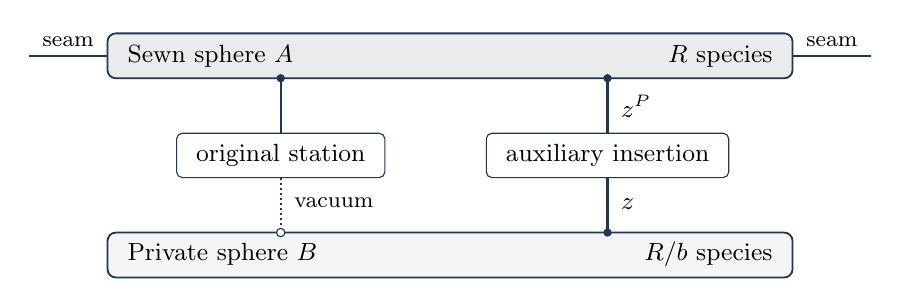
\begin{tikzpicture}[x=1cm,y=1cm,font=\small,
  strip/.style={draw=ink,rounded corners=3pt,line width=.65pt},
  ins/.style={draw=ink,rounded corners=2pt,fill=white,inner xsep=7pt,inner ysep=4pt},
  leg/.style={draw=ink,line width=.8pt}]
\draw[strip,fill=ink!10] (-4.35,.98) rectangle (4.35,1.55);
\draw[strip,fill=ink!5] (-4.35,-1.55) rectangle (4.35,-.98);
\node[anchor=west] at (-4.22,1.26) {Sewn sphere \(A\)};
\node[anchor=east] at (4.22,1.26) {\(R\) species};
\node[anchor=west] at (-4.22,-1.26) {Private sphere \(B\)};
\node[anchor=east] at (4.22,-1.26) {\(R/b\) species};
\draw[leg] (-5.35,1.26)--(-4.35,1.26);
\draw[leg] (4.35,1.26)--(5.35,1.26);
\node[above,font=\footnotesize] at (-4.85,1.26) {seam};
\node[above,font=\footnotesize] at (4.85,1.26) {seam};
\node[ins] (sta) at (-2.15,0) {original station};
\node[ins] (aux) at (2.0,0) {auxiliary insertion};
\draw[leg] (sta.north)--(-2.15,.98);
\draw[leg,densely dotted] (sta.south)--(-2.15,-.98);
\node[anchor=west,font=\footnotesize] at (-2.1,-.6) {vacuum};
\draw[leg] (aux.north)--(2.0,.98);
\draw[leg] (aux.south)--(2.0,-.98);
\node[anchor=west] at (2.05,.62) {\(z^P\)};
\node[anchor=west] at (2.05,-.62) {\(z\)};
\foreach \x/\y in {-2.15/.98,2.0/.98,2.0/-.98}
    \fill[ink] (\x,\y) circle (1.5pt);
\draw[draw=ink,fill=white] (-2.15,-.98) circle (1.5pt);
\end{tikzpicture}
\caption{The station table encodes its incident internal wire bits on \(A\).
The auxiliary tables couple \(A\) to \(B\) and together impose equality
along the wires. Only \(A\) is sewn to neighboring cells.}\label{fig:stack}
\end{figure}

A mark at $z$ on $B$ corresponds to the mark at $z^P$ on $A$, where $P$
is a power of the characteristic. Moving $z$ by $t$ moves $z^P$ by $t^P$.
In units of the Laurent order on $A$, the energy of the pair is therefore
$e_A+P^{-1}e_B$. A given energy budget allows $P$ times as much energy
on $B$. We keep the corresponding leg narrow by using fewer species on
$B$. This will bound the width left behind when a station crosses a seam.

Fix $g,\ell$ as in Lemma~\ref{lem:local}. Let $F$ be the first
characteristic power at least $D^{1000(\ell+1)}$ and let $a=\lceil F^3\rceil$.
For a chunk count $M$ and a sufficiently large characteristic power $b>F$,
take $R$ to be the largest multiple of $bM$ at most $T/a$. Set
\begin{equation}\label{eq:plant-scales}
 R'=R/b,\qquad P=b/F,\qquad \kappa=P^{-1},\qquad H=Ra^2 .
\end{equation}
Here $R$ and $R'$ count the species on $A$ and $B$, respectively, and
$T/(2a)\le R\le T/a$ for sufficiently large $T$. If $e_A+\kappa e_B\le h$,
Equation~\eqref{eq:local-width} bounds the widths by constant multiples
of $\sqrt{Rh}$ and $\sqrt{R'Ph}=\sqrt{Rh/F}$. In bits, up to rounding,
\begin{equation}\label{eq:plant-widths}
 w_A=O\bigl(T\sqrt{h/H}\bigr),\qquad
 w_B=O\bigl(T\sqrt{h/(FH)}\bigr).
\end{equation}

\subsection{The wiring form for one species}

Combine the wires between each pair of distinct stations into one ordered
bundle, absorbing endpoint permutations into the station tables. Contract
self-loops in those tables first. Split each internal bundle into packets
of $R$ bits, padding the last packet with zeros. Species $s$ will carry
bit $s$ of every packet. A station meets $O_g(D)$ bundles, and a cell
together with its incident edges meets $O_g(D^2)$. At a station of
arity $t_i$, one species therefore carries at most $t_i/R+O_g(D)$ bits.

Choose distinct wedge basis states at an integer energy $h_i$ to encode
the bit strings at station $i$. The logarithm of the single-species
dimension is asymptotic to $(\pi/\sqrt3)\sqrt{h_i}$ through integer
levels by Lemma~\ref{lem:dimension}. Since $R\ge T/(2a)$ and $a\ge D$,
we may take
\[
                 h_i=O_g\bigl(a^2(1+t_i/T)^2\bigr).
\]
At seam $j$ the packets across the interface contribute
$O_g(DT/R+D^2)=O_g(Da)$ bits to one species. An integer energy
$q_j=O_g(D^2a^2)$ suffices. The two cells use the same bit order and
the same basis codes there. For fixed $D$ the packet counts per
species, energies and codes range over finite sets.

Define the multilinear form $L$ on these station and seam levels by
its coefficients. Give a basis tuple coefficient one if all codes are
valid and both ends of every bit agree. For a wire to another cell,
compare its station end with its seam end. Every other coefficient
is zero. We will sew a multispecies seam at a fixed \emph{total}
energy. To recover the correct energy in each individual species,
put $Q=\sum_j q_j$ and extend $L$ by zero to all other tuples of
nonnegative half-integer seam energies of sum at most $Q$. The station
energies stay fixed.

\begin{lemma}[Auxiliary marks of bounded weight]\label{lem:plant-probes}
Inserting a joint state at polynomially many extra marks on a
single-species sphere realizes the extended form $L$. At each extra
mark the state uses only the vacuum and $\psi_0$. In every word in its
support the number of occupied marks is even and at most $O_g(Da)$.
\end{lemma}
\begin{proof}
A wedge of length $d$ has energy at least
$\tfrac12+\tfrac32+\cdots+(d-\tfrac12)=d^2/2$. At the stations the
total length is $O_g(a\sum_i(1+t_i/T))=O_g(Da)$. At the at most $g$
seams the same bound follows from Cauchy--Schwarz and their total
energy bound $Q=O_g(D^2a^2)$. List all pairs $(v,m)$ of original
marks and modes occurring in the resulting input spaces. The list
has polynomial size in $D,a$.

An insertion of $\psi_0$ at a new point $z$ pairs with those modes by
the covector with coordinates $(z-z_v)^{-m-1}$. Distinct principal
parts give linearly independent rational functions in every
characteristic. Choose distinct regular points whose covectors span
the dual mode space. Indeed, a nonzero linear combination annihilated
by the points already chosen is nonzero at some unused point of the
algebraic closure. At most one point per listed mode is needed, all
in a finite extension. Add vacua if necessary to obtain at least
three auxiliary marks.

For a subset of $d$ new marks, insert $\psi_0$ there and the vacuum
at the others. Consider first the part of the resulting Pfaffian
in which every auxiliary generator pairs with an original generator.
This part is itself a linear combination of insertion tests on at
most $d$ marks. Indeed, order all auxiliary generators last and group
the matchings by their exact set of internal auxiliary pairs. Each
nonempty set contributes its contracted scalar, with a sign depending
only on those paired positions, times the part on the remaining marks
with no internal auxiliary pairs. Subtracting these contributions
inductively isolates the desired part.

Now take a nonzero vector in the even part of the direct sum of input
spaces, and let $d$ be its greatest nonzero total wedge length. A test
on $d$ marks with no internal auxiliary pairs vanishes on every shorter
wedge. On the length-$d$ component it evaluates the exterior product of
the chosen $d$ covectors, up to a common sign. The original basis
tuples are distinct basis wedges in the exterior algebra on the list
of pairs $(v,m)$. Some choice of $d$ covectors therefore detects the
component. The resulting even tests span the full dual of the even
part. Each actual insertion used has even weight at most $d=O_g(Da)$
and vanishes on odd vectors. The prescribed integer energies give
even lengths, so the zero extension of $L$ also vanishes on the odd
part. A linear combination of insertion tests now gives the required
joint state.
\end{proof}

Use one copy of this state in each of the $R$ species. At station $i$
the insertion table enforces level $h_i$ in every species, decodes the
packets, checks that padded bits are zero and supplies the original
table entry, with its exposed bits. At seam $j$ we sew by basis
equality at total energy $Rq_j$. To see why this recovers the original
wiring, group the Pfaffian by species. Order the original and auxiliary
marks in two consecutive lists and reorder each list by species.
The auxiliary reordering sign can be absorbed in the joint state.
Interleaving the lists costs no further sign because every species
has even auxiliary weight. The original reordering sign depends only on
the input wedges. In any nonzero product after the auxiliary state has
been contracted, the seam tuple of each species
is either the prescribed tuple or has sum greater than $Q$, by the zero
extension. The sums over all species add to $RQ$, so every species
has the prescribed tuple. All the original wedges then have even
length and the remaining reordering sign is one. The product tests
exactly the equality of the bits along each wire. We also place one
vacuum collector in each cell for the motion step.

\subsection{Realizing the joint auxiliary state}\label{subsec:plant-private}

Lemma~\ref{lem:plant-probes} prescribes one tensor shared by all
auxiliary marks. For motion we need a separate insertion table at
each mark. The private sphere supplies the shared tensor through
local maps. One $B$ species will serve a block of $b$ species on $A$.

Partition the $R$ sewn species into $R'$ consecutive blocks. A block
has \emph{type} $\tau=(d_i)_{i=1}^m$ if $d_i$ of its modes $\psi_0$
are occupied at auxiliary mark $i$. Projecting the block tensor onto
these local subspaces gives a tensor $J_\tau$, including the sign
for reordering within the block. Its $i$th leg has dimension
$\binom b{d_i}$. For a fixed ordered word of block types, the joint
tensor is the product of the $J_\tau$ up to a known sign. Exchanging
two site lists from different blocks contributes only the product of
their lengths modulo two to the sign exponent. Retain the types with
$J_\tau\ne0$.

Write $H_2$ for binary entropy in bits, with $H_2(0)=H_2(1)=0$.
Round each $H_2(d_i/b)$ up to a strictly larger point $u_i$ of a
fixed positive grid of mesh $1/m$. Then
\begin{equation}\label{eq:plant-ent}
 \log_2\binom b{d_i}\le b u_i,\qquad
 \max_i u_i\le 2,\qquad \sum_i u_i=O_{g,\ell}(Da\log D).
\end{equation}
Indeed, Lemma~\ref{lem:plant-probes} gives $s=\sum_i d_i/b=O_g(Da)$.
Concavity bounds the sum of the entropies by $s\log_2(em/s)$,
with value zero at $s=0$. The $m$ marks are polynomially many in $D$
for fixed $\ell$ and characteristic, and rounding adds at most one
to the sum.

At the corresponding $B$ marks, take the direct sum $S_\tau$ of all
nonzero single-species sphere forms with energy at most $C(bu_i)^2$
at site $i$, where $C$ is an absolute constant chosen below. For
sufficiently large $b$ there is a constant $c_\tau$ such that for
every $d\ge1$ a product of local linear maps gives
\begin{equation}\label{eq:plant-comparison}
 \bigoplus_{s=1}^{c_\tau} S_\tau^{\otimes d}
                    \longrightarrow J_\tau^{\otimes d}.
\end{equation}
The independence of $c_\tau$ from $d$ will let one selector index
serve every occurrence of the type.

For the comparison, take natural logarithms and work over the
algebraic closure, where the exponent is still strictly below $9/4$.
For a normalized spectral price at $x_1,\ldots,x_m$ put
$M_u=\inf_o\sum_i u_i\,d(o,x_i)$. Preparing $J_\tau$ at $o$ and
transporting its legs bounds its price by $b(\log 2)\sum_i u_i d(o,x_i)$
by Equation~\eqref{eq:plant-ent}. Taking the infimum gives $b(\log 2)M_u$. Applying the same transport bound to
the size-two diagonal, whose price is $\log 2$, gives
$\inf_o\sum_i d(o,x_i)\ge1$. Hence $M_u\ge\min_i u_i>0$.
Apply Corollary~\ref{cor:universal} at scale $N=b$ with width caps
$c_0\sqrt C\,u_i$. Its comparison tensor is precisely $S_\tau$,
whose price is $b(c_0\sqrt C\,M_u+o(1))$ uniformly in the normalized
price.
Choose $c_0\sqrt C>2\log 2$. For fixed $D$ there are finitely many
grid vectors and choices of $A$ positions, all defined over a fixed
finite extension. Taking $P$th roots permutes that field, so the
possible $B$ positions also range over a finite set as $b$ varies.
It follows that $S_\tau$ strictly dominates $J_\tau$ in every price
for all sufficiently large characteristic powers $b$.
The field-extension and strict comparison results of
Section~\ref{sec:prices-background} give Equation~\eqref{eq:plant-comparison}
over the fixed field of definition. The maps extend to the field of
the input tables.

Fix the type word. For each type of multiplicity $d>0$, expand the
restriction in Equation~\eqref{eq:plant-comparison} by choosing one
copy index $s$ and one $B$-energy tuple for each of the $d$ factors.
Assign the factors to private species in the original block order.
Their product is the multispecies sphere form up to the sign for
permuting the homogeneous lists. Each site map now supplies a local
table coupling the $A$ and $B$ legs at that mark. It may act jointly
on all blocks of a given type \emph{at that mark}. Summing the choices
and type words produces the required auxiliary tensor. The $B$ legs
at the original stations and seams stay in the vacuum.

\paragraph{Control and storage.}
A \emph{private selector} records the ordered type word, the
per-block $B$ energies and one index $s$ per occurring type. A single
table checks validity, including zero padding of unused slots, and
supplies the permutation sign. The types and twice the energies cost
$O(m\log(2b))$ bits per block, since $d_i\le b$ and the doubled
energies are $O(b^2)$. The copy indices cost $O_{D,b}(1)$ bits in
total. With $R/b$ blocks, choosing first $b$ and then $T$ large makes
the selector shorter than $\epsilon T$ for any fixed $\epsilon>0$.

On $A$ every occupied auxiliary mode costs energy $1/2$, giving
total auxiliary energy $O_g(RDa)$. On one $B$ species the sum of
the caps is $O(b^2\sum_i u_i^2)=O_{g,\ell}(b^2 Da\log D)$ by
Equation~\eqref{eq:plant-ent}. Multiplying by $R'$ and converting to
$A$ units gives the cell bound
\[
 \sum_i(e_{A,i}+\kappa e_{B,i})
    =O_{g,\ell}(RDa+F RDa\log D)\le D H
\]
for sufficiently large $D$, since $H=Ra^2$ and $a\ge F^3$.
For storage, use the actual spaces of the selected block. At mark $i$
either leg needs only $O(bu_i+1)$ bits, by
Equations~\eqref{eq:plant-ent} and~\eqref{eq:local-width}.
Over all blocks, each auxiliary insertion needs $O(R)=O(T/a)$ bits
for these two legs. Summed over the marks, this costs
$O_{g,\ell}(DT\log D)$, taking $b\ge m$ to absorb rounding.

The selector is summed inside the network, but the outer layout must
know the energy and width at each mark. Split the blocks into $M$ equal
consecutive chunks. In the outer sum, specify for each chunk the
histogram of its pairs (type, $B$-energy tuple). A histogram records
the multiplicities of the pairs, while the private selector records
their order. The alphabet is fixed independently of $T$, so the
histograms cost $O_{D,b,M}(\log(T+1))$ bits per cell. They fix the
energy and the concatenated code length of each leg in each chunk.
The table checks the histograms against the selector and uses its block
order to decode. Each valid selector occurs in exactly one outer term.
Thus $M$ can be chosen for the chunk layout, then $\epsilon$ for its
selector routing, and finally $b$ for the comparison and selector width,
all before $T$ grows.

\section{Moving insertions through a sewn surface}\label{subsec:motion}

The planting construction expresses the original tables on pairs of
spheres in each cell. We now combine these tables at a small number
of marks. Two outcomes of a Laurent expansion suffice. At an insertion
mark, a coefficient fuses the moving table with the table already
there. At a seam, a sufficiently negative coefficient transfers the
moving table to the neighboring cell and lowers the energy of the
seam. This decrease bounds both the number of crossings and the amount
of energy that any cell can receive.

In each cell, designate the marks of the original immobile stations
and one additional vacuum mark as \emph{collectors}. They stay in their
cell. Process the original movable stations in turn, skipping those
already absorbed. The moving table keeps its ordinary bit ports. If its
current legs on the sewn sphere $A$ and private sphere $B$ have
energies $m_A,m_B$, put
\[
       m=m_A+m_B/P,\qquad \mu=m+H,\qquad L=\lceil 2P\mu\rceil .
\]
Here $P$ is the exchange rate of Equation~\eqref{eq:plant-scales}.
The reserve $H$ stays with this move from its start until it ends, while
$m$ is updated after every fusion or crossing.

\subsection{Reconstructing an evaluation from collisions}

Fix the branch of the outer sum and, for the following identity, the
private selectors. The branch determines the energies, so the same
identity works for all allowed selector values. Hold all other positions
and insertion tables fixed. Each entry of the contraction is a rational
function of the mover's $B$-coordinate $z$. Its $A$-coordinate is $z^P$.
The sphere kernels have poles only at other marks on the current sphere
and are bounded at infinity. Near a mark with $B$-coordinate $z_0$, write
$s=z-z_0$. Since $P$ is a power of the characteristic, the corresponding
coordinate difference on $A$ is $s^P$. Hence an $A$-fusion of order $i$
and a $B$-fusion of order $v$ contribute to order $j=Pi+v$ of the
contraction. At an insertion of weighted energy $m_0$ the merged energy is
\begin{equation}
            m_{\rm new}=m_0+m+j/P.                     \label{eq:motion-fusion}
\end{equation}
Indeed each fusion adds its order to the two incident energies, by
Proposition~\ref{prop:fusion}. Nonnegativity of the two output energies
bounds $i$ and $v$ below. Thus the pole orders are bounded, and only
finitely many pairs $(i,v)$ contribute at each $j$.

To reconstruct the value at the current position, use the following
coefficients at the other marks of the cell.
\begin{itemize}
\item at every insertion, its entire principal part;
\item at the designated vacuum collector, also the orders $0,\ldots,gL$,
even after this collector has absorbed a table;
\item at each seam, only the orders $j\le -L$ within its pole bound.
\end{itemize}
A function on which all these coefficients vanish has poles only at the
at most $g$ seams, of order at most $L-1$ each. It has a zero of order
at least $gL+1$ at the designated collector and no pole at infinity.
The degree of the divisor of a nonzero rational function on the projective
line is zero, so this function vanishes identically. On the space with
the prescribed pole bounds, evaluation at the mover's position is
therefore a linear combination of the listed coefficients. This
combination acts entrywise, independently of the tables.

A coefficient at an insertion is a sum over the compatible pairs
$(i,v)$. For each pair, apply the two fusion maps and contract them
with the moving and stationary tables, including the sign of their
chosen order. A collision with a collector ends the move. At any
other insertion only $j<0$ is used, so the combined table continues
with at most the sum of the two original weighted energies. This step
can absorb an auxiliary insertion, an original station awaiting its
turn, or a private insertion left by an earlier crossing.

\subsection{Crossing a seam}

Suppose the selected coefficient has order $j\le-L$ at a seam of
energy $e$. Only sphere $A$ is sewn there. The insertion on $B$ at the
seam is the vacuum, so the $B$-expansion has Taylor orders $v\ge0$.
For each such $v$ with $i=(j-v)/P$ integral and in the fusion range,
the new $A$-energy at the seam satisfies
\begin{equation}
       e'=e+m_A+i\le e+m_A-2\mu\le e-\mu .             \label{eq:motion-drop}
\end{equation}
Terms with $e'<0$ vanish. With $i$ fixed, interpolate the $B$ Taylor
coefficient using evaluations at fresh regular positions. Each resulting
term has one private insertion of energy $m_B$ left behind, with
vacuum on $A$. Its index is carried to the original table by an ordinary
equality wire. We call this private insertion the \emph{residue} of the
crossing.

To identify the new moving table, fix its old $A$-state $x$ by
linearity. Let $a,b$ range over wedge basis states of energies $e,e'$,
respectively, and denote the two remaining sphere forms by
$C_{\rm near},C_{\rm far}$, suppressing their spectator arguments.
Lemma~\ref{lem:seam} gives the identity
\[
\begin{aligned}
 &\sum_b C_{\rm near}(b)\sum_a [I_{e'}(a,x)]_b\,C_{\rm far}(a)\\
 &\hspace{1em}=\alpha\sum_{t\le m_A}\sum_b C_{\rm near}(b)
                      \sum_a [I_e(b,S_t x)]_a\,C_{\rm far}(a).
\end{aligned}
\]
On the right, the inner sum is the Laurent coefficient of order
$e-e'-t$ for an insertion $S_t x$ approaching $b$ on the far-side
$A$-sphere. This order is integral, since $e'-e-m_A=i$ and $m_A-t$
are integers for nonzero terms. Interpolate the coefficient by far-side
regular evaluations, with vacuum in the corresponding $B$-position.
The sum over $b$ sews the two spheres at energy $e'$. The new moving
table, now on the far side with energies $(t,0)$, retains its ordinary
ports and the wire to the residue (Figure~\ref{fig:motion-crossing}).
All reordering signs depend only on the specified energies, and the
identity remains valid when $x$ is coupled to the private index or to a
spectator.

\begin{figure}[!htbp]
\centering
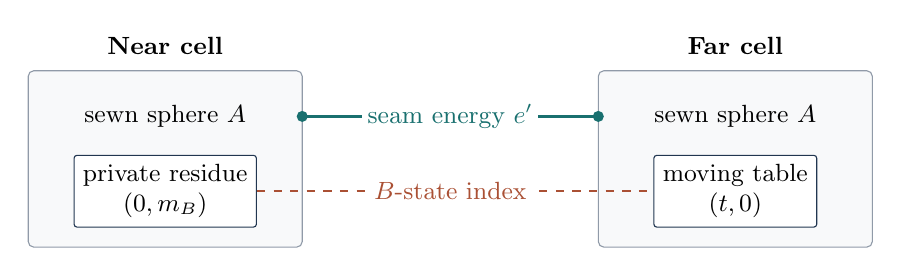
\begin{tikzpicture}[x=1cm,y=1cm, font=\small,
 cell/.style={draw=ink!50,fill=ink!3,rounded corners=2pt},
 tab/.style={draw=ink,fill=white,rounded corners=1pt,inner sep=3.2pt,
             font=\small,align=center}]
 \node[font=\small\bfseries] at (-3.62,1.45) {Near cell};
 \node[font=\small\bfseries] at (3.62,1.45) {Far cell};
 \draw[cell] (-5.36,-1.11) rectangle (-1.88,1.13);
 \draw[cell] ( 1.88,-1.11) rectangle ( 5.36,1.13);
 \node[align=center] at (-3.62,.55) {sewn sphere $A$};
 \node[align=center] at ( 3.62,.55) {sewn sphere $A$};
 \fill[sea] (-1.88,.55) circle (2pt);
 \fill[sea] ( 1.88,.55) circle (2pt);
 \draw[sea,line width=.9pt] (-1.88,.55) -- (1.88,.55);
 \node[fill=white,inner sep=2pt,text=sea] at (0,.55) {seam energy $e'$};
 \node[tab] (res) at (-3.62,-.40) {private residue\\ $(0,m_B)$};
 \node[tab] (mov) at ( 3.62,-.40) {moving table\\ $(t,0)$};
 \draw[dashed,rust,line width=.75pt] (res.east)--(mov.west);
 \node[fill=white,inner sep=2pt,text=rust] at (0,-.40) {$B$-state index};
\end{tikzpicture}
\caption{A moving insertion of energies $(m_A,m_B)$ crosses from the near
cell to the far cell. The solid wire identifies seam states of energy $e'\le e-\mu$. The dashed
wire carries the old private state to the new moving table, whose sewn
energy is $t\le m_A$.}
\label{fig:motion-crossing}
\end{figure}

Both interpolations can be made over the same finite field $K$ as the
original contraction. Multiplying by a common denominator embeds the
space of rational functions bounded at infinity with prescribed poles
into the polynomials of degree at most the total pole bound. Evaluation
at more than that many regular field points is injective, so these
evaluations span the dual and recover each required Laurent coefficient.
Exclude all occupied positions. The map $z\mapsto z^P$ permutes $K$, so
regular evaluations can use corresponding positions on both spheres.
The accounting below bounds the degrees by $O_D(T)$ and the number of
occupied positions per cell by a polynomial in $D$. One can first
obtain those bounds over the algebraic closure and use them to choose
$K$ before any interpolation. Fix an ordering of the field
elements and, for each allowed set of regular points in this order,
store the entries of one reconstruction matrix in the table dictionary. The local control need only
name the selected point and check its availability.

Allow at most $U=D^5$ crossings in a move. When this limit is reached,
its current mark becomes a collector. Nonterminal fusions between
successive crossings remove one stationary insertion each. A completed
move never releases a new mover, so this procedure terminates in every
summand.

\subsection{Accounting for motion}

We first bound the energy stored in the final insertions. An original
station of arity $t_i$ has initial weighted energy $O((1+t_i/T)^2H)$.
The auxiliaries contribute at most $DH$ per occupied cell. Also allocate
one reserve $H$ to each original movable station. The initial insertion
energy and reserves are $O(D^2H)$ per cell. Over all cells, including
all networks in the batch, the bound is
\[
 O\!\left(H\left(D\,\#\{\text{occupied cells}\}
                  +\#\{i\}+T^{-2}\sum_i t_i^2\right)\right)
       =O(WH/T).
\]

A continuing fusion cannot increase the sum of participating energies,
by Equation~\eqref{eq:motion-fusion}. Keep only the reserve of the
current move. In a crossing the energy $m$ pays for $t\le m_A$ on the
far side and $m_B/P$ at the near-side residue. At a final fusion the
collector may gain up to $m+gL/P\le(1+3g)\mu$, since $H\ge1$ and
$P\ge1$. Count energy at collectors with weight $1/(1+3g)$ and energy
elsewhere, including reserves, with weight one. The sum cannot
increase at any of the three operations or when a move expires. The
total insertion energy in every resulting summand is consequently
$O_g(WH/T)$.

There is also a bound in each cell. A crossing brings in at most
$t+H\le\mu$ of charge. By Equation~\eqref{eq:motion-drop} the seam loses
at least this much energy. A cell has at most $g$ seams, each initially
of energy $O_g(D^2H)$. Adding the initial charge within the cell bounds
its current insertion energy by $O_g(D^2H)$ at every step. Moreover,
each crossing decreases the seam energy by at least $H$, so throughout
the construction a cell has $O_g(D^2)$ crossing incidences. Only these
incidences can introduce new stationary residues. With $H=O_D(T)$ and
$P$ fixed, these energy and mark bounds give the asserted $O_D(T)$ total
pole bound. The number of expired moves over all cells is at most the
total number of crossings divided by $U$. Including the initial immobiles
and designated collectors, the total number of collectors is $O(W/(DT))$.

It remains to route the ordinary wires created in the expansion. By
Equation~\eqref{eq:plant-widths}, the private state left at a crossing
uses $O_g(DT/\sqrt F+1)$ bits. One endpoint follows the mover. The
other stays at the residue until another insertion absorbs it, then
travels with that insertion. A residue that can still be absorbed
carries only the endpoint created at its own crossing. Once a moving
endpoint finishes a move, its collector stays fixed. A move visits at
most $U+1$ cells counting repetitions, collecting at most $O_g(D^2)$
residue endpoints per visit and creating at most $U$ of its own.
Hence it carries $O_g((U+1)D^2)$ endpoints along any one hop. Using
the bound on incident crossings and including terminations gives the
looser bound $O_g((U+1)D^6)$ local wire segments per cell. Successive
motions within a single cell require only one local connection. With
$F$ from Section~\ref{subsec:planting}, these segments have total width
$O(D^{-2\ell-1}T)+O_D(1)$ there.

The private-selector wires start at marks that read them and at the
stations checking the selectors and evaluating the sphere forms. Their
endpoints follow the same paths. Each cell starts with polynomially
many such ports in $D$ and the number of chunks, so the path and
crossing bounds give a polynomial bound in the same quantities on
incident selector segments and copies. This count is independent of
$b$ and of the selector rate. After fixing the number of chunks, choose
the rate small enough that the total selector width, including equality
copies, is at most $D^{-2\ell}T$ per cell. The next section converts the
remaining energy levels into table arities.


\section{Accounting for the new arities}\label{subsec:local-output}


After the motion, each collector has two homogeneous sphere legs and may
also hold external bits or thin wires. A seam can still have large energy.
We divide the species into groups so that each group meets a small table,
even when one group receives the entire energy of a seam.

Choose \(M\), a power of \(D\) specified below. Both species counts
\(R,R'\) can be taken divisible by \(M\) in
Equation~\eqref{eq:plant-scales}. Divide the species of each sphere
into \(M\) consecutive equal chunks, preserving whole blocks in the
private construction. Expand each remaining homogeneous leg as a
direct sum over its tuple of chunk energies, using the prescribed tuple
at each untouched auxiliary insertion and the same tuple on both sides
of a seam. Every basis state occurs once in this expansion. For fixed
chunk energies, the sphere form factors into the chunk forms.
Reordering the generators contributes a single sign determined by the
parity of each chunk at each site.

Consider a generic leg of energy \(e\) on \(r\) species, and write
\(e_j\) for the energy in chunk \(j\), so \(\sum_j e_j=e\).
By Equation~\eqref{eq:local-width} and Cauchy--Schwarz, the total
coded width satisfies
\begin{equation}\label{eq:local-chunk-size}
 \sum_{j=1}^M\left\lceil\frac{c_0}{\ln 2}\sqrt{(r/M)e_j}\right\rceil
 \le \frac{c_0}{\ln 2}\sqrt{r e}+M .
\end{equation}
A layout can use the integer width \(\lceil4\sqrt{(r/M)e_j}\rceil\)
instead. This amounts to a rounded integer square root since \(2e_j\)
is an integer, and the same bound holds with coefficient four.

An untouched auxiliary
leg uses the actual product subspace specified by its selector. Within a
chunk, the total number of bits can be read from the counts of block types
and block energies, since a block of type \((d_i)_i\) with rounded entropy bounds
\(u_i\) needs at most \(O(bu_i)\) bits on leg \(i\). Under a fixed selector these codes inject
into the corresponding tensor product of homogeneous spaces. The table
for the chunk form decodes them and assigns weight zero to unused words.

One arbitrary table implements the form at each cell and chunk on the
first and, separately, the private sphere. The number of legs in a cell
is polynomial in \(D\). Equation~\eqref{eq:local-chunk-size}, applied
to a single chunk, bounds a generic port there by \(O(DT/\sqrt M+1)\),
and the bounds on actual auxiliary subspaces give \(O(R/M+1)\) per
auxiliary leg and chunk. Thus the total arity at one of these tables is
at most \(D^{c_1}T/\sqrt M+O_D(1)\), before the small selector wires
are supplied. The exponent \(c_1\) can be chosen independently of
\(M,b\) and the selector rate. Take \(M\) to be a sufficiently large
power of \(D\) to put this quantity below \(D^{-\ell}T/10\). Use
selector rate small enough for the routing bounds of
Section~\ref{subsec:motion} with this \(M\), then choose the block
size \(b\) in the planting. This order permits all three choices to be
made before \(T\) grows.

\paragraph{Frozen stations.}
The collectors become the frozen stations. At one collector of weighted
energy \(e\), the total width of its two sphere legs is
\(O(T\sqrt{e/H})+O(M)\) by Equations~\eqref{eq:plant-widths}
and~\eqref{eq:local-chunk-size}. The motion bounds give
\(\sum e=O(WH/T)\) over all collectors and \(e=O(D^2H)\) at any
one of them. Thus the energy term in the width has squared sum \(O(WT)\)
and maximum \(O(DT)\). The sum over collectors of the squares of their total external widths
is controlled by the input bound, since every immobile retains its own
external ports. All additional wires from motion and selectors together
have total width \(O(D^{-2\ell}T)\) per cell. Their squared widths added at
collectors cost at most \(O(D^{-4\ell}T^2)\) per cell, even if all
end at the same collector. Additive rounding costs from constantly
many chunks, with \(D\) fixed, obey the same bounds for sufficiently
large \(T\). Combining the three charges using
\((x+y+z)^2\le3(x^2+y^2+z^2)\) proves the squared-arity bound, including
the original external widths. The collector count and Cauchy--Schwarz give
\[
 \sum_{\rm frozen}t_i\le
 \left(O\!\left(\frac W{DT}\right)\,O(WT)\right)^{1/2}
 =O(W/\sqrt D).
\]

\paragraph{Core stations.}
To bound the total arity at the chunk tables, first sum their port widths
over all chunks. Untouched auxiliary insertions have total coded width
\(O(DT(1+\log D))\) per cell by Section~\ref{subsec:plant-private}.
The seams have at most \(g\) ports per cell of total width \(O_g(DT)\)
after summing over chunks in Equation~\eqref{eq:local-chunk-size}.
A cell also has \(O_g(D^2)\) residual private legs. Each costs
\(O_g(DT/\sqrt F)+O(M)\) across all chunks by
Equations~\eqref{eq:plant-widths} and~\eqref{eq:local-chunk-size},
so all residual legs together cost \(O(T)\) per cell for large \(T\).
Legs paired with collectors contribute at most the global frozen arity.
The ordinary wires from motion, the selector wires, and any scalar
tables contribute \(O(T)\) per cell. Thus core arity before controlling the host
degree is \(O(W(1+\log D))\). Untouched auxiliaries have individual
arity \(O(T/a)\), the residues have individual arity
\(O(DT/\sqrt F)\), and the chunk tables and routing wires have each been
made smaller than \(D^{-\ell}T\) by a fixed margin. These and the
selector checks exhaust the core tables.

To build a common host, reserve slots in each cell for each kind of
table and bundle that can occur simultaneously in a single summand.
This requires \(D^{O(1)}\) slots per cell. The block size changes table
entries and selector lengths, while the same slots serve every block
type. Combine scalar factors in their cell. Initially allow all
connections between slots in the same cell or in neighboring cells.
Split any direct connection between collectors with a core identity table
on the thin wire carried along their paths. For each core station, attach a fixed balanced binary tree with one
leaf per possible bundle. Its root receives the table's ordered ports,
and each internal vertex separates its list of bits into the sublists
destined for its two children. The corresponding equality tables pass
each bit along a unique path of length \(O(1+\log D)\) and no internal arity exceeds
twice the original station arity. This proves the asserted degree and
total core bounds. Finally take \(c\) larger than the exponents in these
counts by a margin depending on \(\ell\). Padding a nonempty bundle to
\(\lceil T/D^c\rceil\), or making this minimum charge for any one
station, then uses at most \(O(D^{-2\ell}T)\) extra bits per cell.
Unique zero padding preserves the tensor. It also absorbs any bounded
number per cell of weight-only tables in these counts. This proves the first three
conclusions of Lemma~\ref{lem:local}.

\paragraph{Indices of the outer sum.}
Encode each bundle by its endpoint slots, its length, and its position
in the ordered ports at its ends. The input label already includes any local permutation of bits. No individual exterior address is
needed when a bundle is carried as an ordered list. The branching data
at one occupied cell comprise the initial chunk histograms, the motion
and fusion choices (positions, energies, interpolation points and
orders), and the final chunk splittings. Their number of entries is
bounded for fixed \(D\), including the size of the alphabet of the
histograms. Each integer ranges over \(T^{O_D(1)}\). A field point
uses \(O_D(\log T)\) bits. All private selector bits are wires inside
the summand and are excluded from this count. Zero unused entries
give a unique padding of a term index.

Use the supplied coloring of the \((4D^5+20)\)-th power of the host.
Greedy coloring gives such a coloring with \(O_D(1)\) colors for
fixed \(g\). Start motions successively by color and station slot. Concurrent motions affect disjoint neighborhoods,
since each has at most \(D^5\) crossings. A complete padded schedule
therefore has length bounded in terms of \(D,g\) only. In each step
the cells may send their local descriptions to their neighbors. A
merger concatenates the descriptions of its two input tables and the
operation parameters. A crossing adds the named interpolation, the
fusion, and the new endpoints of its thin wire. The history of any
resulting table draws on a bounded number (depending on \(D\)) of
these records. Thus a label of length \(O_D(A+\log(T+1))\) specifies
each entry as a function of its ports through the fixed dictionary.
The dictionary may use arbitrary interpolation weights, restriction maps
and internal contractions. Generating its labels requires no
evaluation of its entries.

It remains to check that the short computations never require inspecting
the selector bits. Counts in a chunk histogram fix the energies and
coded widths. Range and total checks admit every realizable histogram;
the selector check gives zero whenever an admitted histogram is
unrealizable. Interpolation may use a fixed ordered collection of all
regular field points and weights indexed by the local pole bounds.
The scheduler only checks avoidance of marks, the ranges of the indices,
and the rules of fusion and motion. Zero coefficients may be retained.
The checks and length estimates use arithmetic on
\(O_D(\log(T+1))\)-bit integers or field coordinates, including division
with remainder and rounded square roots. The scheduler copies old labels
as strings in fixed padded slots. At each cell the number of records and
operations on them is bounded independently of \(T\), giving
\(O_D(A+(1+\log T)^{O(1)})\) bit operations and bits communicated.
This proves the final conclusion of Lemma~\ref{lem:local}.


\par\needspace{13\baselineskip}
\part{From arity to network volume}\label{part:volume}
\section{Reducing the total arity of a tensor power}\label{sec:rounds}

The concentration estimate of Lemma~\ref{lem:local} divides a network
into a few large stations and a core of small stations. To lower the cost
of evaluating the network we must also reduce the \emph{total} arity.
Indeed, if $u_v$ is the arity at station $v$, the batched evaluation in
Lemma~\ref{lem:batch-table} costs, per tensor copy, at most a constant
times the number of stations plus
\[
       \sum_{v:\,u_v>0}u_v^p
           \le \bigl(\max_v u_v\bigr)^{p-1}\sum_v u_v .
\]
Here $1<p<2$. We can therefore afford some growth in the largest arity
if enough incident bits disappear. The construction below makes this
trade repeatedly, keeping a bound on the sum of squared arities so that
each new network again meets the concentration hypothesis.

Throughout this part $k$ is a finite field with $\omega_k<9/4$, and
logarithms are binary. A \emph{table network} over a field $K$ has bit
wires and a table $\{0,1\}^{s}\to K$ at each station of arity $s$. Its
size is the number of stations plus the sum of their arities, including
external legs. Parallel bits between two stations form an ordered
\emph{bundle}. A label names the station's table in a dictionary fixed
for the network.

\needspace{12\baselineskip}
\begin{lemma}[Compression of a tensor power]\label{lem:macro}
Let $h=\lceil\log_2 n\rceil$, $0<\delta\le 1/10$, and
$0<\beta\le b\le 1/2$. For every sufficiently small fixed $a>0$
depending only on $k,\delta,\beta$, and all sufficiently large $n$, the
following holds. Work over an extension $K/k$ of degree $O(\log h)$
large enough for Lemma~\ref{lem:local} at the scales used below.
Suppose that an input table network has maximum arity $h^b$ or less,
$(\log h)^{O(1)}$-bit table labels, size at most $m$ with
$n\le m\le n^{1.1}$, and $e\le m h^{-2a}$ external bits. Some
$d$ with $1\le d=n^{o(1)}$ admits a table network over $K$ for its
$d$th tensor power, with all $de$ external bits separately accessible,
such that
\[
 \begin{aligned}
 \text{size}&\le md\,h^{-(1-\delta)a},&
 \text{maximum arity}&\le h^{b+(1+\delta)a}.
 \end{aligned}
\]
The output labels again have $(\log h)^{O(1)}$ bits. The cutoff for $n$
may depend on the fixed exponent in the input label-length bound.
\end{lemma}

Call one application of Lemma~\ref{lem:macro} a \emph{macro}.
Before the macro the lookup bound is $O(mh^{b(p-1)})$ per copy.
After it, the bound acquires the factor
\[
       h^{-a\{(1-\delta)-(1+\delta)(p-1)\}} .
\]
Since $p<2$, choosing $\delta$ small makes the exponent negative.
Section~\ref{sec:shaving} accumulates this saving before evaluating the
tables.

\begin{table}[bp]\centering
\small
\begin{tabular}{@{}ll@{}}
\toprule
Quantity & Meaning within one summand\\
\midrule
$H,\ N_b$ & positions of the common host and blocks using it\\
$r$ & number of blocks combined at each grouping step\\
$S,\ T_0$ & initial blocks and original copies per block, with $d=ST_0$\\
$L,\ T$ & total arity budget and working arity scale\\
$D$ & concentration parameter, fixed for all rounds\\[2pt]
$X,\ Z$ & width between core stations and total frozen charge\\
$\Delta,\ \nabla$ & degree bounds for the core host and the full host\\
$B,\ u$ & maximum packing load and unit of internal width\\
\bottomrule
\end{tabular}
\caption{Parameters for the compression of a tensor power. The budgets
$L$, $X$ and $Z$ each cover all blocks of the summand.}
\label{tab:macro}
\end{table}

The macro expands a power of the original tensor as a sum of products.
Each product has many factors, called \emph{blocks}. We combine blocks
in groups of $r$ to pack stations or rearrange their wires. Each round
first concentrates the squared arities, then uses a fixed number of
wire reductions to shorten the core, and finally restores bounded
degree so the next round can start. A wire reduction, called a
\emph{beat}, consists of several contractions followed by a reset of the
core degree. The number of rounds grows with $h$. Once $D$ is fixed,
all repetition counts \emph{within} a round are constant. Table~\ref{tab:macro} collects the budgets and the quantities they measure.

Different summands can use different wirings. The bounds in
Sections~\ref{sec:rounds}--\ref{sec:full} apply to each summand.
Section~\ref{sec:assembly} represents their sum on one fixed network
and completes the proof of Lemma~\ref{lem:macro}.

\subsection{The common graph and its initial loads}
Each summand is a product of \emph{blocks}, with disjoint lists of
external bits. In a single summand its $N_b$ blocks use the same simple
graph of possible adjacencies, the \emph{host}. An occurrence is a
pair consisting of a host position and a block. It can be empty. Each
actual internal wire joins stations in the same block, and the local
port order tells which bits at its ends correspond. Thus a host edge can
carry different bundles in different blocks. We permit the host to depend
on the summand.

At a grouping step, relabel the blocks and group them $r$ at a time, with
$r$ a power of two. In each group the old blocks are multiplied and
transformed together. New positions may be indexed by an old position, a
dyadic subinterval of the $r$ indices, and a bounded number of other
choices. There are fewer than $2r$ intervals. If $H$ denotes the number
of host positions, the padding allowed in any one step will have
\begin{equation}\label{eq:round-occurrence}
 H'\le c rH, \qquad N_b'=N_b/r,
\end{equation}
where $c$ is fixed throughout all repetitions of that step. Constants here
may depend on the round design. Transformations at a single position using
a fixed number of slots can be included in the adjacent grouping step.

At the beginning of each round, every live occurrence holds one station.
The host has degree bounded by an absolute constant, and external bits are fixed at
specified ports. With $T$ a dyadic width and $L$ a total arity budget,
the charged arity of each live station of actual arity $s_v$ is
$z_v=\max(s_v,\theta T)$, where $\theta>0$ is a small fixed dyadic
constant chosen below. Our invariants are
\begin{equation}\label{eq:round-invariants}
 \sum_v z_v\le L,\qquad \sum_v z_v^2\le LT,\qquad
 \max_v z_v\le DT/2 .
\end{equation}
All three bounds cover all blocks of the summand. The first pays for
surviving bits. The second is the input to the next local concentration,
and the third lets us pack several stations without overflowing one
cell. The floor $\theta T$ also bounds how many table descriptions can
enter a pack of a given charge. Remove every scalar station and retain
its entry as a factor of the summand.

First replace the input by a graph of bounded degree. On the ports of
each station of positive arity $s$ use a balanced binary tree. The root
receives its $s$ bits as a bundle, and an identity at each split divides
one ordered bundle in two, of lengths differing by at most one. Place
an identity at each leaf and attach the original wires and external bits
at the leaves. Connecting two of the resulting leaves also handles an input
wire that was a loop. The arities on either end of a tree edge have bounded
ratio. The leaf-to-leaf connections have matching unit width. There are
$O(\log(2+h))$ levels and $O(m\log(2+h))$ total arity. All the new
tables have short labels.

Choose a dyadic $T_0\in[4h^b,8h^b]$. Stack $T_0$ copies of the network
just constructed. At a station of arity $s$ let $v$ be the largest dyadic
integer at most $T_0/s$. Divide the copies into consecutive intervals of
length $v$. Give each interval its own position carrying the product of
the corresponding tables. Its arity $sv$ belongs to $(T_0/2,T_0]$.
Comparable arities on the two ends of each old edge imply that each
interval meets only boundedly many intervals at the other end. Each edge inherits the order of the old bundle and then of the copies,
so its two endpoints use the same bit order. The stacked graph has
bounded degree and $H_0=O(m\log(2+h))$ positions, since a station of
arity $s$ gives at most $2s$ intervals. The table at an interval is
specified by the old table label, the interval length, and a bounded
number of ordered port lengths.

Take $S$ blocks of this stack and pad $H_0$ to order $m\log(2+h)$.
Include the $d$th power of the product of the removed input scalars as
a factor of the final tensor. The starting parameters are
\begin{equation}\label{eq:round-start}
 d=T_0S,\qquad T=T_0,\qquad L=L_0=CmT_0S\log(2+h).
\end{equation}
The total charged arity is at most $L_0$ for a sufficiently large
absolute $C$. Each station has arity in $(T_0/2,T_0]$, so its square
is at most $T_0$ times its arity. This gives all three bounds in
\eqref{eq:round-invariants}. The $ed$ exterior bits retain their
individual names throughout the construction.

\section{Reducing the width between unfrozen stations}
\label{subsec:core-width}

After concentration, some stations remain frozen for the rest of this
round. The others form its \emph{core}. We shall reduce the width
between core stations before restoring bounded degree and passing all
the stations to the next round. Each core occurrence carries one
tensor. Each frozen occurrence holds a list of tensors and the charge
assigned to each when it was frozen. All exterior legs are on frozen
tensors. We discard host adjacencies between frozen stations, since they
carry no wires.

Let \(X\) be the sum, over all blocks, of the widths of the core--core
wires, counting each wire once. Let \(Z\) be the total frozen charge.
The core--frozen wires, called \emph{tethers}, have total width at most
\(Z\). For packing, give each core occurrence load equal to its arity
and each frozen occurrence load equal to the sum of its charges times
a fixed dyadic factor in \((0,1]\). Write \(B\) for an upper bound on
one load. The sum of all loads satisfies \(\mathcal M\le 2X+2Z\).
Each internal width is a multiple of an integer \(u\le B\).

The host records possible contacts across all blocks. Write \(\Delta\ge3\)
for a bound on its core degree and \(\nabla\ge\Delta\) for a bound on
its full degree. A core station can meet different frozen stations in
different blocks, so even a core of degree three can have many potential
tethers. The width estimate below is uniform in their number.

\begin{lemma}[Reduction of core width]\label{lem:core-width}
Fix a bound on the incoming core degree and assume the hypothesis of
Theorem~\ref{thm:sort}. There is a fixed sequence of grouping and
contraction steps, called a \emph{beat}, with the following bounds
in each summand, for slack \(\sigma>0\).
\[
 X_{\rm out}\le \tfrac12 X+C(Z+\sigma),\qquad
 \Delta_{\rm out}\le3,\qquad Z_{\rm out}=Z.
\]
The identity retains all exterior legs separately. The maximum load,
the reciprocal bundle unit and \(\log(2\nabla)\) increase by at most
fixed factors. These factors and \(C\) are independent of the
incoming full degree.

At a step with \(H\) host positions and \(N_b\) blocks, a power of two,
choose dyadic \(r\mid N_b\). Grouping leaves \(N_b/r\) blocks and uses
at most \(crH\) positions. It suffices to take
\(r\ge c_*\), \(c_*HN_bB/r\le\sigma\) at each step and a starting
unit divisible by the product of the subdivision factors. The
position and slack constants \(c,c_*\) may depend on the degree
bounds at the step in question.
\end{lemma}

A beat consists of several wire-saving subrounds and one reset. Each
subround trades some core width for more possible core contacts. The
reset routes the surviving wires through a core of degree three. We
shall choose the number of subrounds so that their combined saving
pays for this routing.

\subsection{A wiring identity}
Place six parties in the triangular array of Figure~\ref{fig:two-layouts}.
A pair is \emph{permitted} if it lies in one row or one column. The
desired equality wires \(AB\) and \(CD\) lie in neither. We shall express
their product as a sum of networks on permitted pairs and then contract
an entire row or column partition. This leaves a choice of two layouts
for the same summand.

\begin{figure}[htb]
\centering
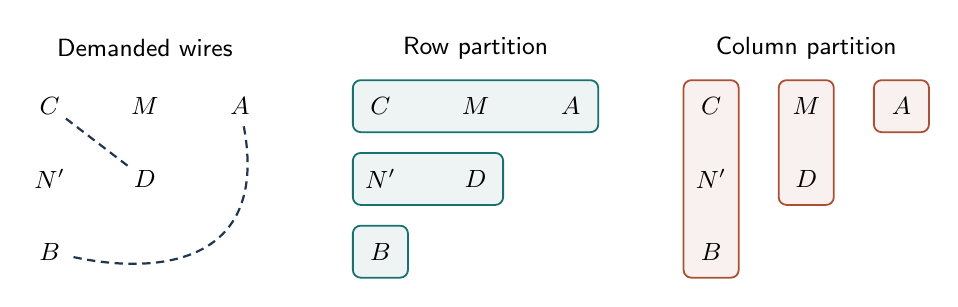
\begin{tikzpicture}[x=1.06cm,y=1.32cm,font=\small,
 party/.style={circle,inner sep=1pt,minimum size=4mm},
 part/.style={rounded corners=2.8pt,line width=.65pt},
 demand/.style={draw=ink,densely dashed,thick}]
\foreach \panel/\shift/\heading in {0/0/Demanded wires,1/4.2/Row partition,2/8.4/Column partition}{
 \begin{scope}[xshift=\shift cm]
 \node[font=\sffamily\small] at (1.14,1.96) {\heading};
 \ifnum\panel=1
  \draw[part,draw=sea,fill=sea!8] (-.33,1.15) rectangle (2.61,1.65);
  \draw[part,draw=sea,fill=sea!8] (-.33,.45) rectangle (1.47,.95);
  \draw[part,draw=sea,fill=sea!8] (-.33,-.25) rectangle (.33,.25);
 \fi
 \ifnum\panel=2
  \draw[part,draw=rust,fill=rust!8] (-.33,-.25) rectangle (.33,1.65);
  \draw[part,draw=rust,fill=rust!8] (.81,.45) rectangle (1.47,1.65);
  \draw[part,draw=rust,fill=rust!8] (1.95,1.15) rectangle (2.61,1.65);
 \fi
 \ifnum\panel=0
  \draw[demand,shorten <=2.6mm,shorten >=2.6mm] (0,1.4)--(1.14,.7);
  \draw[demand,shorten <=2.6mm,shorten >=2.6mm] (2.28,1.4)
    .. controls (2.64,-.14) and (1.26,-.23) .. (0,0);
 \fi
 \foreach \x/\y/\name in {0/1.4/C,1.14/1.4/M,2.28/1.4/A,0/.7/N',1.14/.7/D,0/0/B}{
  \node[party] at (\x,\y) {\(\name\)};
 }
 \end{scope}}
\end{tikzpicture}
\caption{An equality wire between \(C\) and \(M\), for example, disappears
when the rows are contracted and survives when the columns are contracted.
Every permitted wire disappears in one layout. Across all copies of the
identity in a summand, the cheaper of the two common layouts retains at
most half the replacement width.}
\label{fig:two-layouts}
\end{figure}

An \(s\)-bit wire is the equality tensor on the two \(s\)-bit indices.
For a scale-one ordinary price over \(k\), let \(m\) be the greatest
price-distance on a permitted pair. A spanning tree of the permitted
graph supplies one bit shared by all six parties, by equating its
incident bits at each vertex. Thus \(1\le5m\). Both demanded distances
are at most \(2m\). If \(d(C,D)=2m\), the paths \(C,M,D\) and \(C,N',D\)
make \(M\) and \(N'\) the same midpoint in a CAT(0) extension. If also
\(d(A,B)=2m\), then \(C\) and \(M=N'\) are both midpoints of \(A,B\).
This would give \(C=M\) although \(d(C,M)=m>0\). Compactness of
scale-one prices therefore gives a uniform \(\lambda_*<2\) with
\[
 d(A,B)+d(C,D)\le2\lambda_*m .
\]

Choose \(\lambda_*<\lambda_0<2\). For fixed \(\eta'>0\) and arbitrarily
large \(b\), we claim that the two width-\(b\) demands admit an ordinary
sum of at most \(2^{\eta'b}\) networks, each with total permitted width
at most \(2\lambda_0b\). Indeed, choose \(h_0\) large enough that
\(\lfloor2\lambda_0h_0\rfloor>2\lambda_*h_0\). As supply, take the
direct sum over permitted pairs of a single wire on that pair of width
\(\lfloor2\lambda_0h_0\rfloor\). At each spectral point the price of
this supply exceeds that of the two width-\(h_0\) demands. Strict
spectral comparison makes the width-\(b\) demands, for \(b=h_0r\),
a restriction of boundedly many direct copies of the \(r\)th supply power.
Expanding the direct sums and applying the local restriction maps gives
the claimed networks. With \(E_{\rm perm}\) the set of permitted pairs,
a summand index takes \(r\log_2|E_{\rm perm}|+O_{h_0}(1)\) bits.
Choose \(h_0\) and then \(r\) large to fit \(\eta'b\). The identity
over \(k\) extends to every field \(K/k\). For the subround we need a
fixed number of choices even when each wire carries many copies of a bit.

\begin{lemma}[A fixed choice of widths]\label{lem:powered-gadget}
There are constants $b\in\mathbb N$ and $\lambda<2$ such that for
every $z\ge1$ the two width-$bz$ demands are the sum of a bounded
number of networks on the same six parties. Each uses at most
$2\lambda b$ bundles of $z$ bits on permitted edges. Its local
tensors are specified by $z$, the party and the index of the summand.
The index set and choices of widths (in units of $z$) can be fixed independently of $z$.
\end{lemma}

\begin{proof}
Raise the finite identity above to its $z$th tensor power. A term is
initially indexed by a sequence of $z$ selectors, with at most
$\lceil\eta'b\rceil$ bits per selector. For each permitted edge round
up the total number of bits on it to a multiple of $z$. Allowing empty groups, group the
sequences by the vector of rounded numbers in units of $z$. This
vector belongs to a fixed finite set, and rounding costs at most one
unit per permitted edge. Within each group choose a spanning tree
of the connected permitted graph and send the full sequence on each
tree edge, using at most $\lceil\eta'b\rceil$ extra units per edge.
A local table checks identical valid sequences on all incident tree
edges, membership in the group, and zeros in padding positions.
It uses the sequence to split positions on each original edge into
the prescribed slices and evaluates the product of the $z$ local
tables. Connectivity makes the encodings of a sequence unique once
the sequence is specified. Summing the tree variables therefore gives
precisely the sum for that group. The total in units of $z$ is at most
$2\lambda_0 b+|E_{\rm perm}|+5\lceil\eta'b\rceil$. Choose $\eta'$
sufficiently small and then $b$ sufficiently large to bound this by
$2\lambda b$ with $\lambda<2$.
\end{proof}


\subsection{Subrounds}
In a subround we group occurrences at each position into packs. Two
outgoing units from different packs can play the roles \(AB\) and \(CD\).
We first arrange enough such pairs, with a bound on how many packs a
single contraction can merge.

\paragraph{Balanced partitions.}
Within each group of \(r\) block indices use the dyadic intervals in their common order. Give every host edge \(e\) a propagation distance
\[
 s_e=64\lceil\log_2(2x_e)\rceil,\qquad
 x_e=\begin{cases}\Delta&\text{on core edges},\\
                     \nabla&\text{on tethers}.\end{cases}
\]
At each position mark every interval of load greater than \(AB\), with \(2\le A\le r\) dyadic. Marks require splitting. Propagate each mark to its parent at the same position and to its ancestor \(s_e\) levels higher at the other end of each incident edge \(e\), whenever the ancestor exists. The leaves, called colonies, have load at most \(AB\) and length at least \(A\). Intersecting colonies at opposite ends of \(e\) differ in length by a factor at most \(2^{s_e}\), by propagation from the parent of the smaller colony.

A common permutation of the indices inside each group gives a total colony count
\begin{equation}
 Q\le C_1\left( HN_b/r+\mathcal M/(AB)\right)
 \label{eq:core-colonies}
\end{equation}
with \(C_1\) absolute. To see this, identify the indices with \(\mathbb F_r\) in a binary basis and multiply by a uniformly random nonzero element. The probability that two distinct indices fall in one depth-\(j\) interval is at most \(2^{-j}\). At a source position in one group let \(x_i\le1/A\) be the loads divided by \(AB\), and put \(x=\sum_i x_i\). An initially marked interval has at least \(1/2\) in ordered cross products of distinct normalized loads. Thus the expected number of initial marks at depth \(j\) is at most \(2x^2 2^{-j}\). The sum of \(2^{-s_e/16}\) over incident edges is at most \(1/2\) at every vertex. Summing the resulting path weights shows that at most \(2\cdot2^{s/16}\) positions are reachable with total propagation distance at most \(s\). Fix the total upward displacement \(s\), allowing steps to parents at the same position. At each reachable position, depth-\(j\) source marks then reach at most \(2^{j-s}\) distinct ancestors. The expected count there, summed over \(j\ge s\), is at most
\[
 \sum_{j\ge s}\min\{2^{j-s},2x^2 2^{-j}\}=O(x2^{-s/2}).
\]
Summing over distances, sources and groups bounds the number of marks in expectation by \(O(\mathcal M/(AB))\). Each binary partition has one more leaf than marked internal nodes. Choose a multiplier minimizing the actual count.

\paragraph{A wire-saving subround.}
Orient all core edges. Color each block thick or thin, using one affine
functional over \(\mathbb F_2\) on its within-group index. Every position
in a block receives the same color. To pack tensors at one position,
take their tensor product and retain their wires. Any loops created by
later mergers are contracted into the local table. At each core colony gather all thick tensors in one pack. In order, close a thin pack once it reaches load \(B\). There are \(O(A)\) thin packs, each of load at most \(2B\). At a frozen colony concatenate the lists. Let
\(P=2^{64\lceil\log_2(2\Delta)\rceil}\) and \(K_1=\Delta P\).
Pairwise independence of the colors bounds the expected absolute imbalance of thick and thin outgoing widths in a colony by \((B\sum_i a_i)^{1/2}\), where \(a_i\) is the outgoing core amount of its \(i\)th occurrence. Summing gives a coloring of total imbalance at most \(\sqrt{BQX}\).

For a source colony, group thick outgoing units by their destination pack. There are at most \(K_1\) bins by the length ratio along core edges. Treat the outgoing units of each thin pack as one item and match the entire item into any bin with enough remaining capacity. At the first failure every remaining capacity is below \(2B\), so the unmatched part of the smaller total is at most \(2BK_1\). The one-sided matched width therefore satisfies
\[
 I\ge \tfrac12X-\tfrac12\sqrt{BQX}-2BK_1Q.
\]
The colony bound~\eqref{eq:core-colonies} and the slack condition with \(c_*\ge A\) give \(BQ=O((X+Z+\sigma)/A)\). Take \(A\) a sufficiently large dyadic multiple, up to rounding, of \(1+K_1\). Then \(I\ge X/4-O(Z+\sigma)\) with absolute implicit constant.

Within each bin pair its matched thin units with distinct thick units.
Use Lemma~\ref{lem:powered-gadget} with \(b_*=b\) and \(z=u/b_*\), an
integer by the subdivision hypothesis. In each pair the thick wire plays
\(AB\), with \(A\) its source, and the thin wire plays \(CD\), with \(C\)
its source. The sources share a colony. The destinations \(B,D\) belong
to thick and thin packs, respectively, because a wire stays in one
block and the color is common to that block. Introduce fresh auxiliary
parties \(M,N'\) for each pair. Across all pairs, the two demanded
widths have total \(2I\), and the replacement wires have total width at
most \(2\lambda I\) in each product summand.

In one such summand, add the widths that survive the row contractions
over all pairs. Do the same for the column contractions. Every
replacement wire is internal to one of the two layouts, so the two
totals sum to at most \(2\lambda I\). Perform the cheaper contraction
in every pair. Further identifications can only decrease the surviving
width. The unmatched wires contribute at most \(X-2I\), hence
\[
 X'\le X-(2-\lambda)I\le\rho X+C(Z+\sigma),\qquad
 \rho=1-(2-\lambda)/4<1 .
\]

Matching each thin item in its entirety controls the growth in both load and degree. The merged old packs form stars. A thin pack in its source role joins its own thick pack in the row layout or its one chosen thick destination in the column layout. In its destination role it joins only an auxiliary party. Thus one thick center absorbs at most \(O((1+K_1)A)\) thin packs. Every auxiliary is absorbed into a demand endpoint, to which its new incidences can be charged at a constant multiple of the matched width. A dyadic load multiplier \(g\), polynomial in \(\Delta\), bounds both the resulting core loads and the scaled loads of the frozen lists. The new unit is \(u/b_*\).

Reserve pack slots at every potential dyadic interval. Possible core contacts run between packs of one colony or of intersecting neighboring intervals with ratio at most \(P\). There are \(O(P+\log(2P))\) possible intervals per neighbor for each given interval. The stars and the four matched endpoints have bounded diameter in this graph. Taking a fixed graph power gives a common core support of degree at most \(C_2\Delta^{C_2}\). A tether needs just one old tether adjacency with its own length ratio, followed by a bounded number of core adjacencies. Hence the full degree is at most \(C_2\nabla^{C_2}\), with absolute \(C_2\) enlarged if necessary. There are fewer than \(2r\) potential intervals per position. This gives the claimed bound on positions and keeps tethers attached to their respective frozen tensors.

\subsection{Resetting the core degree}\label{subsec:reset}
Use \(H,N_b,\Delta,\nabla\) for the parameters immediately before the
reset, and put \(P=2^{64\lceil\log_2(2\Delta)\rceil}\),
\(K_1=\Delta P\). The reset replaces the core by a degree-three host.
Its principal cost is a permutation network at each core base. Fix a
trivalent network of size \(c_0Yw_0\) that realizes all permutations
of \(Y\) rows of width \(w_0\) by fixing its tags, where \(4K_1\le Y\)
and \(c_0\ge1\). Call this network the \emph{rotor}.

Figure~\ref{fig:reset} shows the two routes. First partition the blocks
at each position into intervals called \emph{bases}, using their mean
loads, and reserve capacity between each pair of adjacent core bases.
Mixing the blocks makes most bases fit these reservations. A wire
between two such bases crosses a direct link between dedicated rotor
outputs. Every core wire incident to an exceptional base takes a longer
route through binary trees. We must bound the total load on those bases
before charging the extra hops.

\begin{figure}[htb]\centering
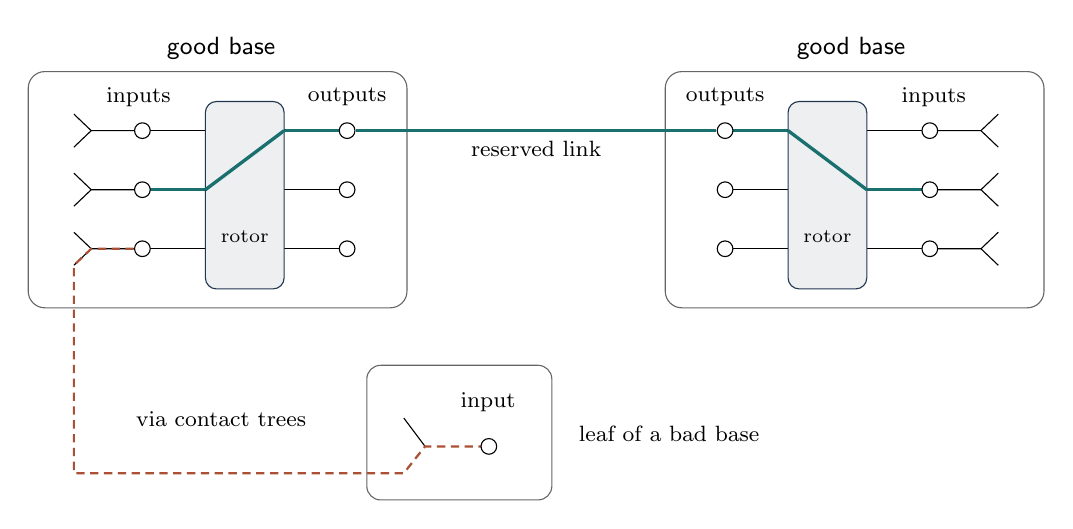
\begin{tikzpicture}[x=1cm,y=1cm,
                        font=\footnotesize,term/.style={circle,draw,fill=white,inner sep=2pt}]
% pair of good bases
\foreach \d/\off in {1/-5,-1/5}{
  \begin{scope}[xshift=\off cm,xscale=\d]
    \draw[draw=black!60,rounded corners=6pt](-1.45,-1.5) rectangle (3.36,1.5);
    \node[font=\sffamily\small] at (1,1.8){good base};
    \node at (-.05,1.18){inputs};
    \node at (2.6,1.18){outputs};
    \foreach \y in {.75,0,-.75}{
      \draw (0,\y) -- (2.6,\y);
      \draw (0,\y) -- (-.65,\y) --(-.87,\y+.21);
      \draw (-.65,\y)--(-.87,\y-.21);
    }
    \draw[sea, very thick] (0,0)--(.8,0) (1.8,.75)--(2.6,.75);
    \draw[draw=ink,rounded corners,fill=ink!8] (.8,-1.26) rectangle (1.8,1.12);
    \draw[sea,very thick] (.8,0) -- (1.8,.75);
    \node[font=\scriptsize] at (1.3,-.59){rotor};
    \foreach \y in {.75,0,-.75}{
       \node[term] at (0,\y){};
       \node[term] at (2.6,\y){};
    }
  \end{scope}}
\draw[sea,very thick] (-2.29,.75) -- node[below,text=black]{reserved link} (2.29,.75);

% link from bottom input on left to a terminal in a bad base
\draw[draw=black!60,rounded corners=5pt] (-2.15,-3.94) rectangle (0.2,-2.23);
\node[anchor=west,align=center] at (.42,-3.1) {leaf of a bad base};
\node at (-.61,-2.7) {input};
\draw (-1.41,-3.26) --(-1.68,-2.9);
\draw[rust,thick,densely dashed] (-5.11,-.75)--(-5.65,-.75)--(-5.87,-.96)
  -- (-5.87,-3.6)-- (-1.68,-3.6) -- (-1.41,-3.26)--(-.6,-3.26);
\node[term] at (-.6,-3.26){};
\node[align=center] at (-4,-2.91) {via contact trees};
\end{tikzpicture}
\caption{Routing during a reset. Between good bases, each end of a
wire reaches a dedicated output through a rotor (solid). A contact
with a bad base joins input terminals through binary contact trees
(dashed). Old tensors and their tethers stay at the inputs. Only
selected terminals are shown.}\label{fig:reset}
\end{figure}

\paragraph{Bases and capacities.}
Choose dyadic $F\ge Y^2w_0$; require $c_*\ge F$ in this step. For the mean load \(\mu_v\) at each position over the \(N_b\) blocks, put
\[
 \nu_v=\max\left\{ FB/r,\ 
      \max_{\pi:y\to v} \mu_y\,2^{-\sum_{e\in\pi}s_e/2}\right\},
\]
allowing a path of length zero. The sum of the attenuated weights of paths from each position is bounded by an absolute constant, as in the colony count. Hence \(\sum_v\nu_v\le HFB/r+C\sum_v\mu_v\). At position \(v\) partition into bases of the largest dyadic length \(s_v\le FB/\nu_v\), between \(F\) and \(r\). All partitions of block indices respect their grouping into consecutive $r$'s. Neighboring base depths differ by at most \(s_e/2\). Their total number is \(O((\mathcal M+\sigma)/(FB))\). For each pair of intersecting bases at neighboring core positions \(v,w\), reserve capacity
\[
 \overline y_{vw}\min(s_v,s_w)+FB/K_1 ,
\]
where \(\overline y_{vw}\) is the mean core amount of that contact per block. The first terms sum to at most \(s_v\mu_v\le FB\) at any base, and there are at most \(K_1\) reservations. Hence total reserved capacity at a base is at most \(2FB\). Base lengths and capacities are fixed from the means before permuting the blocks. In each group the output terminals for a given pair of base positions will therefore occupy the same host slots.

\paragraph{Mixing.}
Permute all block indices by one invertible binary matrix. Within the bases, mark dyadic subintervals (including possibly the bases themselves) of load above \(2FB\), propagating with the same edge distances. Leaves have load at most \(2FB\), length at least \(F\), and the previous length-ratio bounds (base splits above the marked region already satisfy propagation by comparison of the base depths; propagate as in colony packing). Call a base bad if it splits or an incident core reservation overflows. For any \(\delta_*>0\), choosing \(F\) sufficiently large in terms of \(\Delta,Y,\delta_*\) gives a permutation with
\begin{equation}
 \sum_{\text{bad bases}}\mathrm{load}\le\delta_*(\mathcal M+\sigma).
 \label{eq:core-badbases}
\end{equation}
To prove this uniformly in the full degree, count how far one overloaded interval can propagate. For a given position having \(n_v=N_b/s_v\) bases, normalize old loads by \(FB\), obtaining \(x_i\le1/F\). At depth \(j\) below the bases let \(a_J\) be the normalized interval loads and \(\overline a\) their mean, at most \(2^{-j}\). Both \(V_j=\sum_J(a_J-\overline a)^2\) and \(U_j=\sum_J a_J^2-\sum_i x_i^2\) bound the number of overloaded intervals and half their (normalized) load. The prefix collision probability for distinct indices under a random invertible binary matrix is at most the reciprocal of the number of intervals. Consequently
\[
 \mathbb E V_j\le\sum_i x_i^2\le n_v/F,\qquad
 \mathbb E U_j\le n_v2^{-j}.
\]
A mark at depth \(j\) can force a base split only along paths with \(\sum s_e\le 2j\), since neighboring base depths change by at most half the edge distance. For this source mark, dyadic nesting gives at most one affected base at each reachable position. The path count used in~\eqref{eq:core-colonies} therefore bounds the number affected by \(2\cdot 2^{j/8}\). At depth \(j\), use \(V_j\) if \(1/F\le2^{-j}\) and \(U_j\) otherwise. Weight this estimator by \(4\cdot 2^{\lceil j/8\rceil}\). Split the sum at \(j=\log_2 F\). The expected charge is at most a constant times \(n_v\sum_{j\ge0}2^{j/8}\min\{F^{-1},2^{-j}\}=O(n_vF^{-7/8})\). Bases with load above \(2FB\) are paid for directly by the depth-zero estimate. For core capacity overflows use the variance estimator for the contact width divided by \(FB\) at the depth of the base intersections. The \(FB/K_1\) buffer above the mean ensures that each overflow contributes at least \(1/K_1^2\). Summing the unweighted variances in expectation over core edges costs at most \(X/(F^2B)\). Each overflow affects at most two bases. Those whose load exceeds \(2FB\) have already been paid for at depth zero, and every other affected base costs at most \(2FB\). Let \(\Phi\) be the sum of the weighted interval estimators and \(K_1^2\) times the contact variances. We have bounded total bad load deterministically by $O(FB\Phi)$ and have shown
\[
 FB\,\mathbb E\Phi = O(F^{-7/8}(\mathcal M+\sigma)+ K_1^2X/F).
\]
A matrix with estimator at most the mean proves \eqref{eq:core-badbases}. Section~\ref{sec:assembly} finds such a permutation by computing collision scores.

\paragraph{The routes.}
After mixing, group consecutive runs of \(r\) blocks. Give every core leaf \(Y\) input terminals. Assign its old tensors whole to a least-loaded terminal successively, so each terminal receives at most \(2FB/Y+B\le 3FB/Y\). Keep all tethers at their assigned terminals, with their other ends in the concatenated frozen list. For every good core base the rotor connects its input terminals to \(Y\) output terminals. A reservation of capacity \(c\) receives \(\lceil cY/(8FB)\rceil\) pairs of dedicated output terminals, joined by direct links. This needs at most \(Y/4+K_1\le Y\) terminals per base. Divide the units of a good--good contact evenly among its pairs. Their output loads are at most \(8FB/Y+u\le9FB/Y\).

At a good base write \(m_{ij}\) for the number of units routed from input \(i\) to output \(j\). The row and column sums of \((\lceil m_{ij}/w_0\rceil)\) are at most
\[
 9FB/(Yuw_0)+Y\le10FB/(Yuw_0).
\]
Bring every row and column sum to the largest sum by adding edges.
Hall's Theorem decomposes the resulting regular bipartite multigraph
into perfect matchings. Each matching configures a layer of the rotor with bit edges powered to width \(u\). Pin unused inputs and corresponding outputs to zero. Take the tensor product of the layer tables at each rotor position.
This uses only the prescribed equality tensor obtained by pinning the rotor tags. Balanced binary trees at each rotor row collect its \(w_0\) ports, at \(O(\log(2w_0))\) hops per unit. Including direct links this costs \(O((c_0+\log(2w_0))FB)\) per good base.

For a core contact with a bad endpoint use balanced binary contact trees attached to its input terminals. The possible neighboring leaf intervals have length ratios at most \(P\), with \(Y\) terminals per leaf, giving depth \(O(\log(2\Delta Y))\). Route ordered lists through the trees by equality tensors. The assigned lists at both ends give a unique internal assignment to the transmitted bits. Choose \(\delta_*\) in \eqref{eq:core-badbases} small enough to pay this routing depth. Thus for an absolute \(A_0\),
\[
 X'\le A_0(1+c_0+\log(2w_0))(X+Z+\sigma).
\]
This counts every core link in the rotors, collecting trees, direct connections and contact trees. The unit remains \(u\). At every input terminal, output terminal, tree vertex, and rotor vertex the load is \(O(FB)\), as follows from the terminal and layer bounds. For a frozen leaf its scaled list load is at most \(2FB\). The core has degree at most three. Rotor vertices have this degree; input terminals have at most rotor-row (via one edge to a row tree) and contact-tree connections within the core; output terminals have at most a rotor-row connection and a direct link. Each binary tree has degree at most three. For tethers the common host allows every input terminal at every possible intersecting core leaf of the prescribed length ratio. The resulting full degree is bounded by a fixed power of \(2\nabla\), with constants depending on this reset. Reserving this hardware at all possible interval slots costs at most \(c r H\) positions.

\subsection{Paying for the reset}
Write
\[
 \kappa=A_0(1+c_0+\log(2w_0))
\]
for the width multiplier of the reset. Take \(t\) to be the least
positive integer such that \(\kappa\rho^t\le1/2\). Repeated use of the
subround estimate gives core width at most
\(\rho^tX+C(Z+\sigma)/(1-\rho)\) just before the reset. After it,
the coefficient of the incoming \(X\) is at most one half. The
remaining cost is a fixed multiple of \(Z+\sigma\), provided we can
choose a rotor with \(Y\ge4K_1\) for the degree reached after \(t\)
subrounds.

Starting at bounded core degree, the recurrence
\(\Delta'\le C_2\Delta^{C_2}\) gives
\[
 \log_2(4K_1)\le C^{t+1}
      \le C''(2+c_0+\log(2w_0))^{C'} .
\]
Here \(C,C',C''\) depend only on the incoming core degree and the
subround constants. For \(Y=2^y\), Theorem~\ref{thm:sort} gives
\(w_0=\lceil y^{a_\zeta}\rceil\) and \(c_0=O_\zeta(y^\zeta)\) for
each \(\zeta>0\). Fix \(\zeta<1/(2C')\), then take \(y\) large. The
displayed polynomial bound is at most \(y\), so this rotor covers the
required core degree.

The number of subrounds \(t\), the rotor, \(F\) and \(\delta_*\)
depend only on the incoming core-degree bound and the conditional
sorting construction. These parameters bound the growth of the maximum
load. The full degree governs tether propagation and the number of host
positions to reserve. All subrounds together divide \(u\) by
\(b_*^t\), and their polynomial degree bounds, followed by the reset,
multiply \(\log(2\nabla)\) by at most a fixed factor.

This completes the proof of Lemma~\ref{lem:core-width}.


\section{The arity budgets after one round}\label{sec:full}

The frozen stations produced by concentration have total arity
$O(L/\sqrt D)$. The core has small maximum arity but may still use more
than $L$ bits. Repeated beats reduce its internal width until the total
charge fits a smaller budget $L/G$. To resume concentration we will
also need a bound on the squared charges and an absolute degree bound
on the full host.

\subsection{From concentration to bounded degree}
Apply Lemma~\ref{lem:local} with arity exponent $\ell=10$. Its absolute degree bound for the core fixes the parameters of a beat in Lemma~\ref{lem:core-width}. Choose
$\epsilon\in(0,1/100]$ so small that in
\[
 J=\lceil2\epsilon\log D\rceil
\]
beats the products of the per-beat increases of the maximum load, of the
reciprocal bundle unit, and of the logarithm of the overall degree are
each at most $D^{0.03}$ when $D$ is sufficiently large. These three
per-beat factors are independent of $D$, which permits this choice.
Increase $D$ below as needed in terms of $k,\delta,\epsilon$.

We require $ed\le L/D$. For each grouping in this round we also require
\begin{equation}\label{eq:round-slack}
  H N_b T/r\le c_D L
\end{equation}
with $c_D>0$ sufficiently small, using the current host counts and the
round's starting $L,T$. The choices of $S,r$ meeting these conditions
in every round are made below.

\paragraph{Concentrating the squared arities.}
Group $r$ blocks and apply the dyadic partition estimate
\eqref{eq:core-colonies} to the charged loads at absolute host degree,
with maximum load $DT/2$ and capacity $DT$. By
\eqref{eq:round-slack} there are $O(L/(DT))$ occupied intervals over
all positions and groups. Regard each interval as one vertex of the graph
to which we apply Lemma~\ref{lem:local}. Include all candidate intervals
as positions, and allow an edge to an interval at an old neighbor only
when the two intersect and satisfy the absolute length-ratio bound of the
dyadic partition. All actual contacts are present. Dyadic nesting bounds
the simple degree of this new host by an absolute constant.

Inside each occupied interval retain each station of charged arity greater
than $T$. Pack the other stations in their order, closing a pack
when its total charged arity reaches $T$. The last pack can be smaller,
and each pack has arity at most $2T$. Its table is the product of its
members, with any internal indices contracted. An interval contains
$O(D)$ resulting stations. Move its external bits, if any, to one
additional identity station, keeping their order and joining the duplicate
ports to the original incidences. Designate these exterior identities as the immobile stations. Their number is at most the number of occupied intervals. The old stations and packs had total arity at most $DT$ per interval, and the identity adds at most $2DT$. The old large stations contribute at most $LT$ to the square sum. Each new pack has arity at most $2T$, so the packs contribute at most $2TL$.
If $f_i$ is the external width of interval $i$, the new identities
contribute at most
\[
 4\sum_i f_i^2\le 4DT\,ed\le 4LT .
\]
With $W=C_1L$ and $C_1$ absolute and sufficiently large, these are
precisely the occupation, immobility, and square bounds of
Lemma~\ref{lem:local}. In particular there are at most $D$ retained large stations, $D+1$ packs and one exterior identity in an occupied interval, within its bound of $100D$.

Expand using Lemma~\ref{lem:local}. Write $Z$ for the total charged
arity of the frozen stations, and $X$ for the total width of the
internal wires between core stations, counted once per wire. In every
summand the frozen charges have total $Z=O(L/\sqrt D)$, square sum
$O(LT)$ and maximum $O(DT)$. The core stations have individual arities
at most $D^{-10}T$ and total arity $O(L(\log D)^{O(1)})$.
The constants in these estimates are uniform in $D$. All positive
internal bundles have width at least $T/D^{O(1)}$.

To apply the packing operations, take an integer unit $u$ below the
minimum guaranteed internal width, still $u\ge T/D^{O(1)}$, divisible
by every subdivision prescribed in the $J$ beats. For fixed $D$ this is
possible once $T$ is large, by rounding down to a multiple of their
product. Pad each positive internal bundle to the next multiple of $u$
with bits pinned to zero. The arity and its square grow by at most
factors two and four. Raise each frozen charge to the larger of its old charge and its padded arity. Its charge grows by at most a factor of two, so the total $Z$ and the square budget still obey the bounds above. Choose a dyadic load bound $B$ of order
$D^{-10}T$ covering every core station. For packing only, scale the
frozen charges by a fixed dyadic multiplier of order $B/(DT)$, small
enough that each is at most $B$. This changes neither the actual widths
nor the frozen square bound. We take $u$ small enough also to ensure $u\le B$.

\paragraph{Removing the core wires.}
Apply Lemma~\ref{lem:core-width} $J$ times, with slack
$\sigma=L/\sqrt D$. The initial full host degree is polynomial in $D$.
The load bounds at intermediate steps are fixed multiples, depending
only on $D$, of $T$, so \eqref{eq:round-slack} supplies the required
slack each time. In the recurrence of Lemma~\ref{lem:core-width} the fixed error $C(Z+\sigma)$ is multiplied by a geometric series of sum less than two. Thus
\[
 X_{\mathrm{end}}\le 2^{-J}X_{\mathrm{start}}+O(Z+\sigma)
      = O\bigl(LD^{-2\epsilon}(\log D)^{O(1)}\bigr).
\]
Frozen stations retain their charges, although one occurrence can now
hold a list of them. Each list has $D^{O(1)}$ members. Indeed, its total scaled load is bounded by the final load bound, while the positive charge floor gives a lower bound on the scaled load of each member. Each core station has
arity at most $D^{-9}T$. The final bundle unit is still at least
$T/D^{O(1)}$, the core degree is at most three, and the overall degree
$\nabla$ satisfies $\log(2\nabla)\le D^{0.04}$ for $D$ sufficiently
large. The latter estimate uses the initial $O(\log D)$ bound on the
logarithm of the degree.

\paragraph{Restoring bounded degree.}
An individual station can meet few \emph{actual} neighbors and still
have many \emph{possible} neighbors in the common host. At a frozen
position reserve a slot for each member of its list. The only frozen contacts are tethers to the core. Route them in three stages (Figure~\ref{fig:tether-trees}). First
split its active tether units into separate outlets, in order. There
are $D^{O(1)}$ outlets, by the maximum width and minimum unit. Next,
from each outlet use a binary tree addressing any potential core
endpoint. At each core endpoint use a binary tree for the potential
incoming outlets. Link corresponding leaves. An internal branching
table is the identity on the concatenated strings of its active
children. Inactive branches need no station. Each block uses the trees
with precisely its own tether assignments, and the trees and slots
themselves are fixed on the common host. The first trees have depth
$O(\log D)$, and the others have depth
$O(\log(2\nabla)+\log D)=O(D^{0.04})$. Their host size increases
by a factor depending only on $D$. A core endpoint retains at most three
core contacts and receives one tree contact, giving overall degree at
most four.

For the linear budget, the total extra arity is $O(ZD^{0.04})$, since each tether bit travels
along one route of that length. For the square budget, the first splitting tree is bounded in terms of the frozen arity. On a fixed level of that tree
the total width is at most the arity of its frozen station. The
sum of squared arities at that level is at most four times the square
of this arity. Summing first over the frozen stations and then over
levels thus gives $O(LT\log D)$. Every other new vertex carries at
most the width of one unit or all the tether bits of one core station,
so has arity at most $2D^{-9}T$. Its contribution to the square sum
is at most $2D^{-9}T$ times its arity. The old core stations have
total arity at most $2X_{\mathrm{end}}+Z$ and obey the same estimate.

\begin{figure}[tb]
\centering
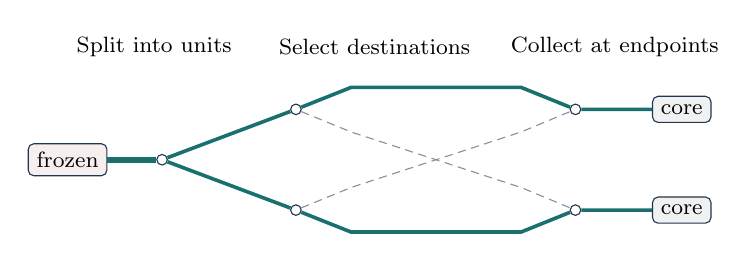
\begin{tikzpicture}[x=1cm,y=.82cm,font=\footnotesize,
  live/.style={draw=sea,line width=1.3pt},
  possible/.style={draw=ink!55,densely dashed},
  branch/.style={circle,draw=ink,fill=white,inner sep=1.35pt},
  station/.style={rounded corners=2pt,draw=ink,inner sep=3pt}]
  \node[station,fill=rust!9] (f) at (0,0) {frozen};
  \node[branch] (split) at (1.2,0) {};
  \node[branch] (a) at (2.9,.78) {};
  \node[branch] (b) at (2.9,-.78) {};
  \node[branch] (c) at (6.45,.78) {};
  \node[branch] (d) at (6.45,-.78) {};
  \node[station,fill=ink!7] (c1) at (7.8,.78) {core};
  \node[station,fill=ink!7] (c2) at (7.8,-.78) {core};
  \draw[live,line width=2.3pt] (f)--(split);
  \draw[live] (split)--(a) (split)--(b);
  \draw[possible] (a)--(3.6,.43)--(5.76,-.43)--(d);
  \draw[possible] (b)--(3.6,-.43)--(5.76,.43)--(c);
  \draw[live] (a)--(3.6,1.12)--(5.76,1.12)--(c)--(c1);
  \draw[live] (b)--(3.6,-1.12)--(5.76,-1.12)--(d)--(c2);
  \foreach \x/\heading in {1.1/{Split into units},3.9/{Select destinations},6.95/{Collect at endpoints}}{
      \node[font=\footnotesize] at (\x,1.75) {\heading};
  }
\end{tikzpicture}
\caption{Two units leave one frozen station. The solid routes are
active in this block. The dashed routes allow either outlet to reach the
other endpoint in a different block. A splitting tree on the left may
carry the full frozen arity for $O(\log D)$ levels. In the middle each
active branch carries a single unit. At the right its width is bounded
by the tether width at the receiving core station.}
\label{fig:tether-trees}
\end{figure}

Together these bounds give charged arities $z_v$ at the end of a
round satisfying
\begin{equation}\label{eq:round-costs}
 \begin{aligned}
 \sum_v z_v&=O\bigl(LD^{-2\epsilon}(\log D)^{O(1)}\bigr),\\
 \sum_v z_v^2&=O\bigl(LT(\log D)^{O(1)}\bigr),\qquad
                   \max_v z_v=O(DT).
 \end{aligned}
\end{equation}
For frozen stations we kept the positive floor from
Lemma~\ref{lem:local}. Every other remaining station meets a positive
internal bundle of width at least $T/D^{O(1)}$. Thus all charges in
\eqref{eq:round-costs} can respect a floor of this order. The constants
and the powers of $\log D$ in \eqref{eq:round-costs} are independent
of $D$. In particular the term $ZD^{0.04}=O(LD^{-0.46})$ fits the
first estimate.

Set $G=2^{\lfloor\epsilon\log D\rfloor}$ and choose a dyadic $q$ with
$G^{1+\delta/4}\le q\le G^{1+\delta/3}$. This interval contains a
dyadic integer for $D$ sufficiently large. Restart with
\begin{equation}\label{eq:round-target}
                 L'=L/G,\qquad T'=qT .
\end{equation}
Indeed $D^{-2\epsilon}(\log D)^{O(1)}=o(1/G)$, and
$L'T'\ge LTG^{\delta/4}$ absorbs the logarithmic loss in the squares.
The maximum in \eqref{eq:round-costs} is at most $DT'/2$ for large $D$.
Finally fix a dyadic $\theta>0$ so small that $\theta qT$ is bounded by
the positive floor just obtained. None of the estimates used in choosing
$G,q,D$ requires a lower bound on $\theta$, since the grouping used the total
load cap and repacked the small stations before applying the local lemma.
This proves \eqref{eq:round-invariants} for the next round.

\subsection{Iteration and the description of the final tables}
\label{iter:subsection}

Fix the round just constructed, including $D$, $G$, $q$ and its $s$
grouping steps. To save a factor $h^a$ in the total charge, take
\[
 j=\left\lceil\frac{a\log h}{\log G}\right\rceil,\qquad
 L_i=L_0G^{-i},\qquad T_i=T_0q^i \qquad(0\le i\le j).
\]
Here $L_i,T_i$ are the budgets after $i$ completed rounds.
It remains to choose $r$ and the initial number $S$ of blocks. A large
$r$ makes partially occupied packs inexpensive. A large $S$ supplies
enough groups for all $sj$ steps and leaves enough blocks to amortize
the common host in Section~\ref{sec:assembly}.

\paragraph{Packing slack and exterior width.}
In one grouping step $N_b$ decreases by $r$ while $H$ increases by at
most $cr$. Their product, which counts allocated occurrences, increases
by at most $c$. The fixed expansions of the host can be included in $c$.
Thus at every stage of the construction,
\begin{equation}
 H N_b\le C^{j+1}mS\log h , \label{iter:occurrences}
\end{equation}
where $C$ depends only on the design of one round. Since
$L_0=C_0 mT_0 S\log(2+h)$, the ratio that controls the slack during
the round starting from $L_i,T_i$ is bounded by
\[
   \frac{H N_b T_i}{rL_i}\le \frac{C_1C^{j+1}(qG)^i}{r}.
\]
Choose $r$ to be the least power of two at least $C_2(CqG)^{j+1}$.
The round design fixes $C_2$ so that this ratio is at most $c_D$ in
\eqref{eq:round-slack} and $r$ meets the lower bound in every step.
In particular $r=h^{O_D(a)+o(1)}$, independently of $S$. The external
width has a separate bound. The $ed$ exposed bits are present in every
round, and $G^j<Gh^a$. Hence for $i\le j$,
\[
       \frac{ed}{L_i}=\frac{eG^i}{C_0m\log(2+h)}
           =O_D\!\left(\frac{h^{-a}}{\log h}\right).
\]
For sufficiently large $h$ this gives $ed\le L_i/D$, the width
allowance for the immobile exterior identities.

\paragraph{Copies and terminal budgets.}
Let $R$ be the least power of two at least $h^M$, for any fixed $M>0$.
Taking $S=Rr^{sj}$ leaves exactly $R$ blocks after $j$ rounds.
Each initial block contains $T_0$ copies, so $d=T_0S$ and
$\log d=O((\log h)^2)$. In particular $d=n^{o(1)}$.
Now $h^a\le G^j<Gh^a$, $q\le G^{1+\delta/3}$ and $T_0=\Theta(h^b)$.
It follows from \eqref{eq:round-start} and \eqref{iter:occurrences} that
\begin{equation}
 \begin{aligned}
 L_j&=O(md\log h\,h^{-a}),&
 T_j&=O\bigl(h^{b+(1+\delta/3)a}\bigr),\\
 HN_b&\le mS h^{O_D(a)+o(1)} .
 \end{aligned}
 \label{eq:round-terminal}
\end{equation}
The occurrence bound holds throughout, with a constant in $O_D(a)$
independent of $M,a,b,\beta$. These scales also justify using a single
working field. They range from $T_0\ge4h^\beta$ to a fixed power of
$h$. Choose the extension degree divisible by the degree of the fixed
extension in Lemma~\ref{lem:local}, and large enough to meet the
cardinality requirement at $T_j$. Its degree is $O(\log h)$ and hence
$O(\log T_i)$ for every $i$.

\paragraph{Descriptions of tables.}
An occurrence carries a label for its table, the widths of its bundles,
and their positions in its port order. The cost of naming its
incident host edges is bounded in terms of $D$ because each edge can
be named by its place in the local neighbor list. Constants indexed by $D$ may depend on the round design. These local data have total length per occurrence at most
\begin{equation}
 C_3^{j+1}(\log h)^{O(1)}
   =h^{O_D(a)+o(1)} .
 \label{iter:labels}
\end{equation}

At initialization the stack at a position has a fixed table label,
specified by its original table, its stack length and the locations
of its ordered sublists. Its description has length
$(\log h)^{O(1)}$. Within one round the following facts bound
the number of old labels that can enter any new label.
\begin{itemize}
\item A colony of capacity $DT_i$ contains at most $D/\theta$ live
entering stations, since each is charged at least $\theta T_i$.
The local expansion in Lemma~\ref{lem:local} uses a bounded number of
old labels, discrete choices and field elements in each output
description. Its additional description length is $O_D(\log h)$.
\item In a subround or reset, both the bound on load per leaf and the
bound on the number of leaves contributing to one resulting pack are
fixed multiples, depending on $D$, of $T_i$ and $1$, respectively.
Each live core contributes at least one internal unit of width
$u\ge T_i/\operatorname{poly}(D)$. The charged load of an individual
frozen station has the same kind of lower bound even after the fixed
rescaling. Scalar stations are withdrawn as soon as they form. It
follows that a contributing pack has a bounded number of old labels
and a bounded number of units. Lists of unit pairings, rotor layers
and ordered sublists at a port therefore have bounded numbers of
entries. Each entry needs at most $O_D(\log h+\log r)$ bits. This
also describes the routing on the final trees at the frozen stations.
\end{itemize}
Thus if $A$ bounds the current label length, one step gives a bound
$C_4A+C_4(\log h)^{C_5}$, including the descriptors of locally
withdrawn scalar factors. The multiplicative constant counts old
labels, independently of the field degree and the length of the input
dictionary labels. Iteration through the $sj$ steps proves
Equation~\eqref{iter:labels}. Global host addresses enter the control
of a whole position only. They never have to be appended to an
individual table description.

\paragraph{The tensor represented by the sum.}
Each term now consists of $R$ surviving blocks and the scalar factors
withdrawn along its history. Regrouping permutes the exterior lists along with their stations and preserves each product entry by entry. A local tensor identity replaces a product by a sum with the same entries on those $ed$ named ports. Colorings, packings, and routings use fixed tie-breaking rules. Only choices from local tensor identities index the expansion.
The final internal wire assignments are summed when the $R$ blocks are
contracted.

For this evaluation one dictionary suffices. A key records the type,
stage, description and arity of a table, followed by its incident bits.
Length fields or fixed padding give a unique encoding. The input
dictionary and the rules of the construction assign a field value
to each valid key. The values at unused keys may be fixed arbitrarily.
In particular, a key for a withdrawn scalar has no incident bits.
A longest key has length
\[
 O_D(T_j)+h^{O_D(a)+o(1)}
\]
by the maximum-arity invariant and Equation~\eqref{iter:labels}.
A derived table description can exceed $(\log h)^{O(1)}$ bits. Section~\ref{sec:assembly} places that description in the \emph{argument} of a dictionary call. The label of the installed table need only specify the key format and length. This accounts separately for the arity of a lookup and the short label required as input to the next macro.


\section{Realizing the expansion on a fixed network}\label{sec:assembly}

Different summands in Section~\ref{sec:full} can finish with different
wires and different tables. To represent their sum on one network, we
encode a choice of summand, together with an assignment to its final
wires, as a transcript. A local check determines which transcripts
contribute, and a dictionary supplies their tensor entries. The size
bound depends on how the host is shared. All blocks at one host
position use the same address. The bits carried on a wire vary
independently across blocks.

\subsection{From a transcript to a tensor}

Let $K$ be the working extension of $k$, and put
$h=\lceil\log_2 n\rceil$. Fix $P\le n^{O(1)}$ numbered processors.
Each has binary advice of at most $h^c$ bits and a fixed ordered list
of exterior ports. Its local record includes guesses and at most
$h^c$ incoming and outgoing messages. A message consists of an
$O(h)$-bit key identifying source, destination and port, together with
a bit string. Communication is valid if every used key occurs exactly
once at each end with the same string.

One fixed finite bit-RAM program checks the local record against the
advice and exterior bits. It may emit strings of length at most $U$ as
arguments to a common dictionary $W$ with values in $K$. Its
decisions depend only on the strings. For fixed exterior bits, the
transcript tensor is the sum over accepted transcripts of the product
of all values returned by $W$. The record format, including length
fields and padding, is fixed. All size-dependent program data enter
through the advice.

The charge at a processor includes its deterministic running time,
advice, exterior bits, guesses, messages with headers, and emitted
strings. Count at least one unit per record or item. This charge is
determined by the record. A local address or time uses
$(\log h)^{O(1)}$ bits. Bit arithmetic on words of that length adds at
most a factor $(\log h)^{O(1)}$ to the bounds below.

\begin{lemma}[Realizing a transcript]\label{lem:fixed-transcript}
Suppose the charge of each local record is at most
$V_{\max}=2^{(\log h)^{O(1)}}$. Let $V\le n^{O(1)}$ bound the total
charge of every accepted transcript and the volume of the fixed
advice and exterior interface, including one unit per processor. If
$U\le h$ and the wide-record bound of Theorem~\ref{thm:sort} holds,
then for every fixed $\tau>0$ the transcript tensor has a fixed
network of size at most
\[
                          h^\tau V+P h^{C_0}.
\]
The gates are trivalent or are dictionary tables of arity
$O(1+U+\log h)$. Their labels use $(\log h)^{O(1)}$ bits. The
constant $C_0$ depends only on $\tau,c$, the polynomial bounds in $n$
and the wide-record estimate. The exponent in $V_{\max}$ occurs only
in factors $(\log h)^{O(1)}$ before absorption.
\end{lemma}

\begin{proof}
\emph{Allocate space by record length.}
For each dyadic capacity $t$, from $1$ to the least power of two
at least $\min(V,V_{\max})$, reserve
$N_t=\min(P,\lfloor 2V/t\rfloor)$ slots. A processor with charge $s$
uses the least $t\ge s$. Every record of this class has charge
greater than $t/2$, so $N_t$ slots suffice. Guess their processor
identifiers and records. Check the identifier range and the charge,
require occupied slots to form an increasing prefix in identifier
order, and pin all unused entries and padding. The two relevant
capacity bounds are
\begin{equation}\label{eq:asm-seats}
 \sum_t tN_t=O\bigl(V(1+\log V_{\max})\bigr),\qquad
 \sum_t N_t=O\bigl(P(1+\log V_{\max})\bigr).
\end{equation}

\emph{Check the computation and its dictionary arguments.}
In a slot of capacity $t$, guess the deterministic execution for at
most $t$ steps. Time-ordered checks verify its instructions, registers,
counter, addresses and halt flag, with fixed padding after halt. To
check the memory trace, sort the reads, writes and initial contents by
address and execution order. Scan each address to verify that a read gives the
most recent value, starting at zero for unused cells. This is the
trace construction of \citet[Section~\ext{G}{app:trace}]{oaG}.
A comparison network on $O(t)$ accesses uses $O(t\log^2(2t))$
comparisons of $(\log h)^{O(1)}$-bit words. Long inputs, advice,
messages and emitted strings occupy addressed arrays and are
processed in pieces. The local cost is $t(\log h)^{O(1)}$ plus
$h^{O(1)}$ per slot for long identifiers and framing.

Within the slot, group the emitted strings by least dyadic padded
length $u$, counting an empty string as length one. Reserve
$\lfloor2t/u\rfloor$ calls in that class and take them in issuance
order. The checker writes each emitted bit at the address given by
its length class, ordinal and bit offset. The same memory-trace test
checks these arrays against the inputs of the installed calls,
including their active flags, actual lengths and zero padding. Each
address has $O(1+\log t+\log h)$ bits. Accounting for all the padded
seats adds $t(\log h)^{O(1)}$ to the checking cost. A seat returns
the value of $W$ on its indicated active string and returns $1$ when
inactive. Its table is named by the padded length. The arity is
$O(1+U+\log h)$ and the total table size per slot is
$O(t\log(2+U)\log(2+h))$.

\emph{Match the messages.}
Fix $w=\lceil h^{C_1}\rceil$, where $C_1>1$ will be chosen for
the wide-record sort. Split each message into $w$-bit chunks, padding
the last one and reserving one for an empty message. Its chunk record
contains an active flag, key, direction, total length, chunk number
and payload. Add a fixed sender for each processor. Its key belongs
to a reserved namespace and supplies that processor's advice and exterior bits with their
component lengths. An occupied slot must receive the whole supply
for its claimed identifier even when the supply is empty.

Check each outgoing source and incoming destination against the slot
identifier, and check the splitting, piece order, lengths and padding. Sort the
records by active flag, key, chunk number and direction. In the active
part, require every key and chunk to occur as one send and one receive
of equal length and payload. A duplicate message on one side collides
at chunk zero. In particular each private supply is matched to exactly
one slot, so every processor occurs once. For a given input the
stable-sort relation has just one output, which can be summed out after
these checks. Its zero-one tensor over $k$ extends to the same relation
over $K$.

A slot reserves $O(t/w+h^c+1)$ chunk records. The $O(h)$-bit header
is copied once per chunk, so constructing them costs
$(t+h^{O(1)})(\log h)^{O(1)}$. Charge a fixed sender for its actual
supply and one partial chunk. By Equation~\eqref{eq:asm-seats} the
reserved bit volume, including padding at message boundaries, is
\[
                     V(\log h)^{O(1)}+P h^{O(1)} .
\]
Pad the list to a power of two. Its length is polynomial in $n$, so
its logarithm is $O(h)$. Theorem~\ref{thm:sort} with tolerance
$\tau/3$ permits a fixed $C_1$ large enough that sorting costs at
most $O(h^{\tau/3})$ times this volume. The subsequent scan has
linear size. Equation~\eqref{eq:asm-seats} gives the same volume
bound for the local computations and the dictionary tables. Absorb
the powers of $\log h$ into $h^\tau$ and the per-processor costs
into $P h^{C_0}$.

The checking and sorting gates are trivalent over $k$, and each
dictionary gate is named by its length class. These names have the
stated length. For each accepted transcript the slot capacities,
identifiers, order, traces, calls and chunks are uniquely specified.
Conversely the local and communication checks recover an accepted
transcript. Contracting the installed relations therefore gives its
weighted sum exactly over $K$.
\end{proof}

\subsection{The transcript of the rounds}

We now apply Lemma~\ref{lem:fixed-transcript} to the expansion in
Section~\ref{sec:full}. Initially there are $S$ blocks of $T_0$
copies, so $d=T_0S$. At every stage of the $j$ rounds there are
$N_b\ge R$ blocks on a host with $H$ allocated positions. Give each
position one processor, including at the terminal stage, and give
each step $O(H)$ more processors for balanced aggregation trees. An
occurrence consists of one position in one block.

\paragraph{One address for all blocks.}
A position holds the ordered list of its host neighbors and an array
of occurrence records in block order. Its advice specifies the
parent and child naming conventions, integer parameters, field
presentation, and the initial convention for ordering exterior ports. At an
initial position it also gives the input table label. Exterior bits
enter through fixed ports in stack order.

In one step every host degree is bounded in terms of the fixed round
design. A ball of radius $O_D(1+\log r)$ thus contains $r^{O_D(1)}$
positions. Exchange neighbor lists to that radius, remove repetitions
by identifier and order the resulting names. This locates each
possible child and contact by an index in a local list, at a cost of
$h^{O(1)}$ common operations per position. A message to a contact
can now carry an entire array of occurrence records under one
$O(h)$-bit header. Within that array only local indices are needed.
There are $h^{O(1)}$ phases and declarations per position. By
Equation~\eqref{iter:labels}, handling the arrays costs
$N_b r^{O_D(1)}(\log h)^{O(1)}h^{O_D(a)}
=N_b h^{O_D(a)+o(1)}$ per position. The coefficients in $O_D(a)$
are independent of $a,b,\beta$.

For decisions shared by the host, each position computes its local
contributions to the candidate scores. Sum the integer arrays along
a balanced tree and broadcast the first minimizing candidate. At
height $i$ the width of a sum of initially $z$-bit entries is at
most $z+i$, while the number of positions falls by a factor of order
$2^i$. Since
$\sum_{i\ge0}2^{-i}(z+i)^{O(1)}=O((1+z)^{O(1)})$, aggregation
preserves the preceding bit-cost bound. At the root allow an
additional $2^{(\log h)^{O(1)}}$ operations to choose the
minimizer. A greedy coloring of a given host can be checked locally
as well. In fixed identifier order, require each color to be the
least one absent from its lower neighbors. Induction on identifiers
makes the checked assignment unique.

\paragraph{Checking the changes of host.}
Each of the operations in a round supplies its contacts from these
neighbor lists and its common parameters from additive scores.
\begin{enumerate}
\item For colony packing, try the multipliers of the $r$ slots,
propagate the overloaded marks to ancestors and neighbors, and sum
the candidate colony counts. A propagation moves upward by at least
one dyadic level, so the radius is $O_D(1+\log r)$. Relative
interval endpoints, loads and dyadically scaled charges all have
short encodings. Summing the local scores also chooses the affine
coloring for whole-item pairing.
\item At a local concentration step, the colony interval and its
old contacts give the possible neighbors of each sphere. In the
checked color order, the movement and interpolation choices of
Lemma~\ref{lem:local} specify the new tables, withdrawn scalars
and ordered bundles. Its description bounds pay for the choices and
labels. The port orders identify the exposed sublists.
\item In a wire-saving subround the source colony and bin determine
the seats of its matched units. Record one summand choice for each
actual gadget. Sum the surviving replacement widths under each of
the two contractions and take the same minimizer for all blocks.
The widths before identifying coincident endpoints suffice for this
decision. Bounded neighborhoods of the colonies then determine the
new contacts, port orders and table labels.
\item For a reset, compute each position's mean load over the blocks.
The smoothed mean has floor $FB/r$ and a propagated contribution
decays by at least a factor of two per edge. The starting load is at
most $B$, so a neighborhood of radius $O(1+\log r)$ determines the
bases and their capacities.

For the common mixer, let $x_i$ be the normalized load at a position
or the normalized width at an edge in block
$i\in\mathbb F_2^{\log_2 N_b}$. At prefix length $s$ the part of
the collision estimator of Section~\ref{subsec:reset} that depends
on a candidate matrix $A$ is a multiple of
\[
 \sum_{z\ne0}\boldsymbol{1}_{(Az)_{1:s}=0}
                     \sum_i x_i x_{i+z}.
\]
Two indices have the same output prefix exactly when their
difference $z$ satisfies the displayed condition. The diagonal and
centering terms are constant in $A$, so they can be omitted in
choosing a minimizer. The denominators of the remaining $x_i$ are
cleared by $FB$ times the fixed dyadic load denominator. The level
and overflow weights are integers after fixed scaling. In
particular the choice uses integer arithmetic in every
characteristic.

Compute the autocorrelations $\sum_i x_i x_{i+z}$ simultaneously by
squaring the Walsh coefficients and inverting the transform. This
takes $O(N_b\log N_b)$ operations on $(\log h)^{O(1)}$-bit local
integers. Aggregate the coefficients by difference and prefix
length. At the root one can enumerate all invertible matrices in
dimension $\log_2 N_b=O((\log h)^2)$ within
$2^{(\log h)^{O(1)}}$ bit operations. The first minimizer satisfies
the bound proved by averaging. Positions permute their block arrays
accordingly. The bounded length ratios of intersecting leaves and
the bounded number of units per leaf then allow the terminal
assignments, rotor settings and new labels to be determined from
neighboring records.
\item The final splitting trees for tethers have bounded size,
depending on $D$, per possible station and contact. Adjacent
positions determine the active sublists. An edge between new
children is supported by a bounded path between their parents. In
the next phase the children use their own host adjacency, so every
neighborhood collected is local to its current step.
\end{enumerate}

Declare messages in a fixed order of phases, ports and blocks.
Enforce each successive array and common host from the preceding
data and the local summand choices. Each term of a local identity,
including a term of weight zero, has one prescribed encoding. The
intermediate arrays therefore introduce no further multiplicities.

\paragraph{Independent bits and tensor entries.}
Transfer the exterior bits in the order specified by the splits and
concatenations. The source and destination share a processor header
for all pieces sent along one contact. Their array positions and bit
offsets have length $(\log h)^{O(1)}$. When a sphere collects bits
at its exterior station, the station is frozen during the ensuing
steps. When the blocks are reordered, permute its lists with them.
Neighborhood collection transports descriptions. Each of the $ed$
exterior bits travels only along its specified route, at most once
per transfer. The $O(\log h)$ steps therefore use
$ed(\log h)^{O(1)}$ payload work.

At the terminal stage, guess one bit per internal wire at its
designated endpoint and send it to the other endpoint in contact
and bundle order. A table call consists of the station description
and its ordered port bits. The terminal payload costs
$L_j(\log h)^{O(1)}$ by Equation~\eqref{eq:round-terminal}.
A scalar withdrawn earlier issues its call at withdrawal, with just
the short description. The input scalars are fixed. If their product
is $c$, one nullary table of value $c^d$ supplies their contribution
to the entire expansion. Naming this element of $K$ costs $O(\log h)$
bits. For fixed summand choices, the free
payload guesses now range exactly over the terminal wire
assignments. The product of call values is their contraction
weight. Summing over these assignments and then over summands gives
the input tensor power on its ordered $ed$ exterior bits.

\paragraph{Size of the fixed network.}
At each stage Equation~\eqref{eq:round-terminal} gives
$HN_b\le mS h^{O_D(a)+o(1)}$. There are $O(\log h)$ steps, and
$N_b\ge R$. The bounds for processors and for their total charge are
therefore
\begin{align}
 P&\le mS h^{O_D(a)+o(1)}/R,\nonumber\\
 V&\le P h^{C_2}+mS h^{O_D(a)+o(1)}
     +(L_j+ed)h^{o(1)}+2^{(\log h)^{O(1)}}.\label{eq:asm-volume}
\end{align}
The first two terms pay for the common work per position and the
short records per occurrence. The third term pays for independent
wire bits, and the last for the root computations. Every local
record has charge at most $2^{(\log h)^{O(1)}}$, since $N_b\le S$,
$\log S=O((\log h)^2)$ and an occurrence has only polynomially many
bits in $h$. The exponent $C_2$ and the exponent bounding the
declaration count can be fixed independently of $M$ in
$R=h^{M+o(1)}$. Common work uses $O(h)$-bit addresses and
$r^{O_D(1)}$ candidate contacts. The dependence on $M$ is confined
to factors polynomial in $\log S$ and the additive root cost.

The longest dictionary call uses $O_D(T_j)+h^{O_D(a)+o(1)}$ bits.
Choose $a$ small enough that $Ca+2a<\beta$ for each coefficient $C$
in the short-work and label bounds, and $b+(1+\delta)a<1$ for all
allowed $b$. Equation~\eqref{eq:round-terminal} gives
$T_j=O(h^{b+(1+\delta/3)a})$, so the calls have length below $h$.
Use Lemma~\ref{lem:fixed-transcript} with $\tau=a\delta/3$, then
take $M$ sufficiently large to absorb both $P h^{C_0}$ and
$P h^{C_2+\tau}$. For the three other charges in
Equation~\eqref{eq:asm-volume}, the costs per $md$ before the
factor $h^\tau$ are
\[
 \frac{mS h^{Ca+o(1)}}{md}=h^{-b+Ca+o(1)},\qquad
 \frac{ed}{md}\le h^{-2a},\qquad
 \frac{L_j}{md}=O(h^{-a}\log h).
\]
Here $d=T_0S$ and $T_0=\Theta(h^b)$. The additive root cost is
$n^{o(1)}$ while $m\ge n$. Consequently the fixed network has size
at most $md\,h^{-a+\tau+o(1)}\le md\,h^{-(1-\delta)a}$ for
large $n$. Its maximum table arity, including the activity and
length fields, is at most $h^{b+(1+\delta)a}$. A dictionary table
retains its short length-class label, ready for another application
of Lemma~\ref{lem:macro}. This completes the proof of that lemma.

\section{Trivalent compression and the exponent}\label{sec:shaving}

Each application of Lemma~\ref{lem:macro} reduces the size per copy and
raises the maximum arity. We stop while the saving in size still exceeds
the cost of evaluating the larger tables. Two operations then recover a
trivalent network over the original field. Batched evaluation uses
Lemma~\ref{lem:batch-table}, and a single coordinate projection removes
the field extension used in the local identities.

\begin{lemma}[Descent of a trivalent network]\label{lem:table-descent}
Let $K/k$ have finite degree $D$. If a trivalent $K$-network of size
$s$ represents a tensor with entries in $k$, the same tensor has a
trivalent $k$-network of size $O(sD^2)$ with the same exterior positions.
\end{lemma}

\begin{proof}
Choose a $k$-basis of $K$ whose first element is $1$. For
$\lambda\in K$, let $M_\lambda$ represent multiplication by $\lambda$
in that basis. Order the stations along a chain and give each of them
two extra ports carrying the incoming and outgoing basis indices.
If an assignment to its original ports has weight $\lambda$, the
enlarged table returns the indicated entry of $M_\lambda$. Pin both
ends of the chain to the first index. For any fixed assignment to the
original wires, contracting along the chain now gives the first
coordinate of the product of the weights. This coordinate map is
$k$-linear. Summing over the original internal bits therefore takes
the first coordinate of the old tensor entry, which belongs to $k$.

Encode each basis index in $\lceil\log_2 D\rceil$ bits, giving weight
zero to unused codes. The enlarged table has at most
$r=3+2\lceil\log_2 D\rceil$ bits. Every table on $r$ bits has a
trivalent realization of size $O(2^r)$. In the binary prefix tree
compute, at each node, the indicator that the input has that prefix.
At depth $j$, copying the next input bit to the $2^j$ nodes and testing
the two children of each node costs $O(2^j)$ gates. Give each leaf a
unary weight equal to its table entry when its indicator is one and to
$1$ otherwise. Exactly one leaf supplies the selected entry. Summing
the level costs gives $O(2^r)=O(D^2)$ per original station.
\end{proof}

\begin{proof}[Proof of Theorem~\ref{thm:shaving}]
Fix the finite field $k$ with $\omega_k<9/4$ and the exterior-bit
allowance $\eta>0$. Write $h=\lceil\log_2 n\rceil$. The ordinary-width
sort in Theorem~\ref{thm:sort} supplies an exponent $1<p<2$. Put
$\rho=p-1$. A total arity increase from $h^\beta$ to $h^{b_*}$ will
cost $O(h^{\rho b_*})$ per surviving incidence in the final lookup.
Choose $0<\delta\le1/10$ so that $1-\delta>\rho(1+\delta)$. Take
$A>0$ sufficiently small, and then $\beta>0$ sufficiently small, that
$b_*=\beta+(1+\delta)A$ satisfies
\begin{equation}\label{eq:shaving-margins}
 b_*<\tfrac12,\qquad \rho b_*<\tfrac12\eta,\qquad
 \Delta=(1-\delta)A-\rho b_*>0 .
\end{equation}
The positive gap $\Delta$ is the net saving on the original network
size. Choose a fixed integer $J$ large enough that $a=A/J$ satisfies
Lemma~\ref{lem:macro} uniformly for $\beta\le b\le1/2$ and
$2a<\eta/2$.

One extension $K/k$ suffices for these $J$ applications. Each width
scale $T$ lies between a constant times $h^\beta$ and a fixed power of
$h$. The local identities require a fixed constant extension and a
field of cardinality at least a fixed power of $T$. Choose $[K:k]$
large enough for the largest such power and divisible by the degrees
of the required constant extensions. Since $k$ is finite, we can do
this with $[K:k]=O(\log h)=O(\log T)$ at every scale.

Let $s_j$ count stations and their total arity after $j$ applications,
let $d_j$ be the cumulative number of copies, and put $e_j=d_j e$.
Initially $d_0=1$, $s_0=O(m)$, the arity is at most $3\le h^\beta$,
and the trivalent $k$-tables have a fixed finite dictionary. At step
$j<J$ use the size allowance
\[
 M_j=\max\{s_j,\lceil e_j h^{2a}\rceil\}.
\]
This allows the construction to continue even when the exterior bits
already account for most of the current size. We have $M_j\ge n$,
$e_j\le M_j h^{-2a}$ and maximum arity at most
$h^{\beta+(1+\delta)aj}$. If this application makes $r_j$ copies,
Lemma~\ref{lem:macro} preserves the short table labels, gives
$d_{j+1}=r_jd_j$ and yields
\[
 s_{j+1}\le r_j M_j q,\qquad q=h^{-(1-\delta)a}.
\]
Its construction in Section~\ref{sec:full} has
$\log_2 r_j=O((\log h)^2)$ uniformly in the input network. Inductively,
the original bound $s_0,e_0=O(n^{1.05})$, multiplied by a fixed
number of these copy factors and fixed powers of $h$, gives
$M_j\le n^{1.05+o(1)}\le n^{1.1}$ at every invocation.

In terms of size per exterior bit, $x_j=s_j/e_j$, the replication
factor cancels. For large $h$,
\[
 x_{j+1}\le q\max\{x_j,2h^{2a}\},\qquad
 x_J\le \max\{q^J x_0,2q h^{2a}\}.
\]
Indeed $q<1$, so every contribution arising from an exterior-bit
allowance is bounded by the most recent such allowance.

Let $u$ be the final maximum arity. Applying
Lemma~\ref{lem:batch-table} makes $2^u$ copies and multiplies the
size per copy by $O((1+u)^\rho)$. The resulting tensor is the
$d$th power of the original $k$-tensor, with
\[
 d=2^u d_J,\qquad
 \log_2 d\le h^{b_*}+O\bigl(J(\log h)^2\bigr)=o(h).
\]
Thus $d=n^{o(1)}$ uniformly at fixed $k,\eta$. Each of its $de$
exterior positions is retained through lookup and through
Lemma~\ref{lem:table-descent}. Descent costs $O([K:k]^2)=h^{o(1)}$.
Combining these bounds, the trivalent size over $k$ divided by $de$
is at most
\[
 O(m/e)\,h^{-\Delta+o(1)}
       +h^{2a+\rho b_*+o(1)} .
\]
Choose $\gamma=\Delta/2$. The strict inequalities
$\Delta>\gamma$ and $2a+\rho b_*<\eta$ absorb the constants and
lower-order terms for large $n$. Multiplication by $de$ gives
Equation~\eqref{eq:shave}.
\end{proof}

For the distinctness tensor of Theorem~\ref{thm:many}, the independent
exterior positions are the entries of separate lists. Choosing
$\eta<\sigma$, Proposition~\ref{prop:finitefield} iterates the
compression until the volume per exterior bit is $O(w^\eta)$, below
the required $w^\sigma$. This rules out $\omega_k<9/4$ over every
finite field. Lemma~\ref{lem:specialize} transfers the lower bound to
any field, where the matching upper bound gives Theorem~\ref{thm:square}.


\bibliographystyle{plainnat}
\bookmarksetup{startatroot}
\bibliography{references}
\end{document}
